\documentclass[]{article}
\usepackage{lmodern}
\usepackage{amssymb,amsmath}
\usepackage{ifxetex,ifluatex}
\usepackage{fixltx2e} % provides \textsubscript
\ifnum 0\ifxetex 1\fi\ifluatex 1\fi=0 % if pdftex
  \usepackage[T1]{fontenc}
  \usepackage[utf8]{inputenc}
\else % if luatex or xelatex
  \ifxetex
    \usepackage{mathspec}
  \else
    \usepackage{fontspec}
  \fi
  \defaultfontfeatures{Ligatures=TeX,Scale=MatchLowercase}
\fi
% use upquote if available, for straight quotes in verbatim environments
\IfFileExists{upquote.sty}{\usepackage{upquote}}{}
% use microtype if available
\IfFileExists{microtype.sty}{%
\usepackage{microtype}
\UseMicrotypeSet[protrusion]{basicmath} % disable protrusion for tt fonts
}{}
\usepackage[margin=1in]{geometry}
\usepackage{hyperref}
\hypersetup{unicode=true,
            pdftitle={Supplemental Information for ``Examining Repressive and Oppressive State Violence using the Ill-Treatement and Torture Data''},
            pdfborder={0 0 0},
            breaklinks=true}
\urlstyle{same}  % don't use monospace font for urls
\usepackage{graphicx,grffile}
\makeatletter
\def\maxwidth{\ifdim\Gin@nat@width>\linewidth\linewidth\else\Gin@nat@width\fi}
\def\maxheight{\ifdim\Gin@nat@height>\textheight\textheight\else\Gin@nat@height\fi}
\makeatother
% Scale images if necessary, so that they will not overflow the page
% margins by default, and it is still possible to overwrite the defaults
% using explicit options in \includegraphics[width, height, ...]{}
\setkeys{Gin}{width=\maxwidth,height=\maxheight,keepaspectratio}
\IfFileExists{parskip.sty}{%
\usepackage{parskip}
}{% else
\setlength{\parindent}{0pt}
\setlength{\parskip}{6pt plus 2pt minus 1pt}
}
\setlength{\emergencystretch}{3em}  % prevent overfull lines
\providecommand{\tightlist}{%
  \setlength{\itemsep}{0pt}\setlength{\parskip}{0pt}}
\setcounter{secnumdepth}{0}
% Redefines (sub)paragraphs to behave more like sections
\ifx\paragraph\undefined\else
\let\oldparagraph\paragraph
\renewcommand{\paragraph}[1]{\oldparagraph{#1}\mbox{}}
\fi
\ifx\subparagraph\undefined\else
\let\oldsubparagraph\subparagraph
\renewcommand{\subparagraph}[1]{\oldsubparagraph{#1}\mbox{}}
\fi

%%% Use protect on footnotes to avoid problems with footnotes in titles
\let\rmarkdownfootnote\footnote%
\def\footnote{\protect\rmarkdownfootnote}

%%% Change title format to be more compact
\usepackage{titling}

% Create subtitle command for use in maketitle
\providecommand{\subtitle}[1]{
  \posttitle{
    \begin{center}\large#1\end{center}
    }
}

\setlength{\droptitle}{-2em}

  \title{Supplemental Information for ``Examining Repressive and Oppressive State
Violence using the Ill-Treatement and Torture Data''}
    \pretitle{\vspace{\droptitle}\centering\huge}
  \posttitle{\par}
    \author{}
    \preauthor{}\postauthor{}
      \predate{\centering\large\emph}
  \postdate{\par}
    \date{15 August 2019}

\usepackage{booktabs}
\usepackage{longtable}
\usepackage{array}
\usepackage{multirow}
\usepackage{wrapfig}
\usepackage{float}
\usepackage{colortbl}
\usepackage{pdflscape}
\usepackage{tabu}
\usepackage{threeparttable}
\usepackage{threeparttablex}
\usepackage[normalem]{ulem}
\usepackage{makecell}
\usepackage{xcolor}

\begin{document}
\maketitle

{
\setcounter{tocdepth}{2}
\tableofcontents
}
\hypertarget{additional-control-variable-choices}{%
\section{Additional control variable
choices}\label{additional-control-variable-choices}}

For additional robustness checks, we considered the following
indicators:

\begin{itemize}
\tightlist
\item
  Media freedom, from Whitten-Woodring and Van Belle (2017), via
  \url{http://faculty.uml.edu/Jenifer_whittenwoodring/MediaFreedomData_000.aspx}.
  Per the authors recommendations we collapsed the 3-valued media
  freedom indicator into a binary ``functionally free'' and ``not free''
  version.
\item
  IGO membership as an indicator of political globalization, from the
  COW IGO state unit dataset (Pevehouse, Nordstrom, and Warnke 2004).
\item
  Linear and squared year trends
\item
  Human rights organization membership (\texttt{hro\_n}) and secretariat
  locations (\texttt{hro\_secloc}). From Murdie and Davis (2012),
  \url{http://amandamurdie.org/research.html}, where the original
  variable names are \texttt{hrfilled} and
  \texttt{HRsecretariatlocation}.
\item
  Trade as \% of GDP as an economic globalization indicator. From the
  World Bank WDI.
\end{itemize}

The trade and HRO data contain missing values. The number of
observations in a model depend on the particular combination of the 3
indicators impacted in a given specification, such that:

\begin{table}[H]
\centering
\begin{tabular}{lrr}
\toprule
Variables & N & Fraction\\
\midrule
None & 1654 & 100\\
NE.TRD.GNFS.ZS & 1552 & 94\\
hro\_n & 1209 & 73\\
hro\_secloc & 1208 & 73\\
hro\_n, NE.TRD.GNFS.ZS & 1136 & 69\\
\addlinespace
hro\_n, hro\_secloc & 971 & 59\\
hro\_n, hro\_secloc, NE.TRD.GNFS.ZS & 947 & 57\\
\bottomrule
\end{tabular}
\end{table}

Since any coefficient estimate differences between a model that includes
one or more of these three variables with missing values and another
without, we decided to not use them. Thus we restrict our sensitivity
analysis to the first three items in the list above.

\hypertarget{sensitivity-analysis}{%
\section{Sensitivity analysis}\label{sensitivity-analysis}}

The conduct the robustness / sensitivity analysis, we followed the
``reasonable specification'' approach outlined in Simonsohn, Simmons,
and Nelson (2015). This is a method that fits in the space between
estimating a limited number of additional models for robustness checks
and extreme bounds analysis where we estimate all possible combinations
of specifications given a set of variables. Instead, they suggest
listing a set of reasonable modeling and specification choices, where
each choice is a decision between two or more alternatives, and then
estimating all combinations of those choices. In the languge of Gelman's
garden of forking paths (2013), we try to follow all paths a reasonable
modeller might take.

In spirit this is a restricted version of extreme bounds analysis, that
seeks to eliminate unreasonable specifications. For example it makes no
sense to estimate a model including both raw and logged GDP, rather we
would only want to examine one at a time.

We included the following choices in our sensitivity analysis:

\begin{itemize}
\tightlist
\item
  Model type: 2 alternatives; either a regular Poisson count model (GLM)
  or a Poisson count model with random country intercepts (GLMER).
\item
  Base terms: 2 alternatives; intercept(s) only or the basic controls,
  as discussed in the main paper.
\item
  Media freedom: 2 alternatives; no control or the global media freedom
  index
\item
  Political globalization: 3 alternatives; no control or a count of IGO
  memberships or the proportion of IGOs in existence in a year that a
  country is member of.
\item
  Year trend: 3 alternatives; no trend, linear trend, or squared trend
\end{itemize}

Altogether this represents 72 possible specifications. The one we report
in the paper is a Poisson GLMER model with random country intercepts,
includes the base control set, but does not include any other control
variables. We examined each of the 72 specifications for each of the 14
variables of interest using each of the 3 dependent variables.

Altogether this comes out to 3,024 estimated models. Simonsohn et al use
specification plots as the first step in interpreting the findings.
Since this still leaves us with 42 specification plots overall (14
variables \(\times\) 3 DVs each), we skip this and first summarize even
further by tallying, for each VOI, the number of coefficient estimates
that are negative and stastistically significant (\(p < 0.05\)),
negative but \(p > 0.05\), positive but \(p > 0.05\) and lastly positive
and significant. This is shown below in Table \ref{tab:sens}, and next
we will highlight findings regarding the main results we present in the
paper. After that will be a section where we show what specification
plots are, followed by a list of all 42.

\begin{table}[t]

\caption{\label{tab:sens}Summary of sensitivity analysis estimates}
\centering
\begin{tabular}{>{\raggedright\arraybackslash}p{3in}lrrrr}
\toprule
\multicolumn{2}{c}{ } & \multicolumn{4}{c}{$\beta$} \\
\cmidrule(l{3pt}r{3pt}){3-6}
\multicolumn{3}{c}{ } & \multicolumn{2}{c}{$p > 0.05$} & \multicolumn{1}{c}{ } \\
\cmidrule(l{3pt}r{3pt}){4-5}
Variable & Outcome & - & - & + & +\\
\midrule
 & Criminal & 66 & 0 & 3 & 3\\

 & Dissident & 72 & 0 & 0 & 0\\

\multirow[t]{-3}{3in}{\raggedright\arraybackslash Democracy, 0/1} & Marginalized & 51 & 0 & 1 & 20\\
\cmidrule{1-6}
 & Criminal & 6 & 18 & 12 & 36\\

 & Dissident & 39 & 15 & 0 & 18\\

\multirow[t]{-3}{3in}{\raggedright\arraybackslash CCP Due process} & Marginalized & 45 & 5 & 4 & 18\\
\cmidrule{1-6}
 & Criminal & 0 & 7 & 18 & 47\\

 & Dissident & 72 & 0 & 0 & 0\\

\multirow[t]{-3}{3in}{\raggedright\arraybackslash CCP Habeas corpus} & Marginalized & 36 & 5 & 26 & 5\\
\cmidrule{1-6}
 & Criminal & 36 & 0 & 0 & 36\\

 & Dissident & 63 & 0 & 0 & 9\\

\multirow[t]{-3}{3in}{\raggedright\arraybackslash CCP Pretrial release} & Marginalized & 36 & 9 & 3 & 24\\
\cmidrule{1-6}
 & Criminal & 36 & 0 & 0 & 36\\

 & Dissident & 64 & 6 & 2 & 0\\

\multirow[t]{-3}{3in}{\raggedright\arraybackslash CCP Speedy trial} & Marginalized & 29 & 25 & 0 & 18\\
\cmidrule{1-6}
 & Criminal & 30 & 13 & 14 & 15\\

 & Dissident & 66 & 6 & 0 & 0\\

\multirow[t]{-3}{3in}{\raggedright\arraybackslash CCP Torture} & Marginalized & 45 & 12 & 13 & 2\\
\cmidrule{1-6}
 & Criminal & 0 & 0 & 0 & 72\\

 & Dissident & 0 & 0 & 0 & 72\\

\multirow[t]{-3}{3in}{\raggedright\arraybackslash EPR Excluded groups (\% of total pop)} & Marginalized & 0 & 0 & 12 & 60\\
\cmidrule{1-6}
 & Criminal & 0 & 0 & 0 & 72\\

 & Dissident & 0 & 0 & 0 & 72\\

\multirow[t]{-3}{3in}{\raggedright\arraybackslash EPR Excluded groups (count)} & Marginalized & 0 & 2 & 26 & 44\\
\cmidrule{1-6}
 & Criminal & 72 & 0 & 0 & 0\\

 & Dissident & 72 & 0 & 0 & 0\\

\multirow[t]{-3}{3in}{\raggedright\arraybackslash VDem Civil liberty social class equality} & Marginalized & 72 & 0 & 0 & 0\\
\cmidrule{1-6}
 & Criminal & 60 & 12 & 0 & 0\\

 & Dissident & 72 & 0 & 0 & 0\\

\multirow[t]{-3}{3in}{\raggedright\arraybackslash VDem Civil liberty social group equality} & Marginalized & 72 & 0 & 0 & 0\\
\cmidrule{1-6}
 & Criminal & 51 & 21 & 0 & 0\\

 & Dissident & 72 & 0 & 0 & 0\\

\multirow[t]{-3}{3in}{\raggedright\arraybackslash VDem Judicial constraints on executive} & Marginalized & 69 & 0 & 0 & 3\\
\cmidrule{1-6}
 & Criminal & 30 & 4 & 32 & 6\\

 & Dissident & 72 & 0 & 0 & 0\\

\multirow[t]{-3}{3in}{\raggedright\arraybackslash VDem Legislative constraints on executive} & Marginalized & 36 & 22 & 11 & 3\\
\cmidrule{1-6}
 & Criminal & 41 & 30 & 1 & 0\\

 & Dissident & 72 & 0 & 0 & 0\\

\multirow[t]{-3}{3in}{\raggedright\arraybackslash VDem Power by social group} & Marginalized & 69 & 0 & 0 & 3\\
\cmidrule{1-6}
 & Criminal & 61 & 11 & 0 & 0\\

 & Dissident & 72 & 0 & 0 & 0\\

\multirow[t]{-3}{3in}{\raggedright\arraybackslash VDem Power by socioeconomic position} & Marginalized & 70 & 2 & 0 & 0\\
\bottomrule
\end{tabular}
\end{table}

\hypertarget{summary-of-findings}{%
\subsection{Summary of findings}\label{summary-of-findings}}

The sensitivity results overall are consistent with the results of the
core specifications reported in the paper. There are some instances
where the sensitivity results are stronger than those reported in the
paper, e.g.~in the same direction but with a larger proportion of
statistically significant estimates (both of the EPR power variables).
And there are some instances where the results tend towards but are not
clearly in the other direction, e.g.~for CCP Habeas Corpus we noted a
negative but insignificant estimate while includes more positive
estimates, although still many insignificant. We note either kind of
divergence below.

\hypertarget{negative-relationship-for-democracy-01}{%
\subsubsection{Negative relationship for ``Democracy
0/1''}\label{negative-relationship-for-democracy-01}}

We report a negative relationship between this and all three outcomes.
This largely holds up, with significant negative estimates in all 72
specs for ``dissidents'', 66 for ``criminal'', and 51 for
``marginalized''

\hypertarget{negative-relationship-for-constitutional-provisions}{%
\subsubsection{Negative relationship for constitutional
provisions}\label{negative-relationship-for-constitutional-provisions}}

Negative relationships for the binary constitutional provision
indicators, except one negative but insignificant estimate for ``CCP
Habeas Corpus'' on ``Criminal'' in the main paper.

In the sensitivity analysis:

\begin{itemize}
\tightlist
\item
  the finding for ``CCP Habeas Corpus'' on ``Criminal'' actually leans
  towards positive or inconsistent (insignificant).
\item
  for the remaining indicators and outcomes, they either tend to be
  consistent with the main paper results, or, when there are deviations,
  they appear to mostly be due to the model and intercept choice.
  Particularly, when using a regular Poisson count model without country
  random effects there are several sign reversals.
\end{itemize}

\hypertarget{positive-relationships-for-epr-excluded-groups}{%
\subsubsection{Positive relationships for EPR excluded
groups}\label{positive-relationships-for-epr-excluded-groups}}

In the paper we note positive effects and that the effect, surprisingly,
appears to be the largest for criminal victims.

These findings hold up well in the sensitivity analysis.

\begin{itemize}
\tightlist
\item
  for ``Marignalized'' victims, there are some insignificant estimates,
  although mostly still with positive point estimates.
\item
  the estimate size is still overall quite large for ``Criminal''
  victims, however, the estimate size for ``Dissident'' victims in the
  sensitivity analyises is generally larger than those in the paper, and
  approaching rough equality with the overall average ``Criminal''
  victims effect sizes.
\end{itemize}

\hypertarget{negative-but-sometimes-insignificant-associations-for-v-dem-indicators}{%
\subsubsection{Negative but sometimes insignificant associations for
V-Dem
indicators}\label{negative-but-sometimes-insignificant-associations-for-v-dem-indicators}}

In the paper, the estimates for the V-Dem variables have negative signs,
except one positive but insignificant estimate (for Legislative
Constraints - Criminal victim type). Four of the negative sign
coefficients do not have statistical significance, the remaining do. The
sensitivity analysis is again largely consistent with these results.

Notable divergences are:

\begin{itemize}
\tightlist
\item
  The negative but insignificant effects for Power by socioeconomic
  position and social group on Criminal victim type are actually more
  strongly negative and significant in the sensitivity analysis.
\item
  For judicial constraints and criminal victim types, the paper
  esetimates are negative but insignificant, whereas in the sensitivity
  analysis the estimates more strongly lean towards clearly negative,
  especially in the global intercept only regular Poisson count models.
\item
  For legislative constraints the paper results are slightly positive
  but insignificant; the sensitivity results are quite divergent. The
  country random intercept Poisson GLMER model produces mostly positive
  but insignificant estimates, while out of the global intercept only
  Poisson GLM's 36 estimates all were significant but 6 with positive
  signs and 30 with negative signs. The 6 Poisson GLM estimates with
  positive signs all exclude the basic controls, i.e. ``Intercept(s)
  only'' and exclude either of the political globalization indictors,
  i.e.~have ``None''. Changing either of those two choices flips the
  sign to negative.
\end{itemize}

\clearpage

\hypertarget{specification-plots}{%
\section{Specification plots}\label{specification-plots}}

The specification plots provide more details than our summary above
does, and also make it possible to identify, to some extent, which
specification choices lead to certain findings. Thus we include them
here for anyone interested in more detail.

\hypertarget{introduction}{%
\subsection{Introduction}\label{introduction}}

This is an example of a specification plot for the indicator of whether
a country constitution includes a due process provision
(\texttt{ccp\_dueproc}) and where the DV is ITT allegations of criminal
torture (\texttt{itt\_alleg\_vtcriminal}).

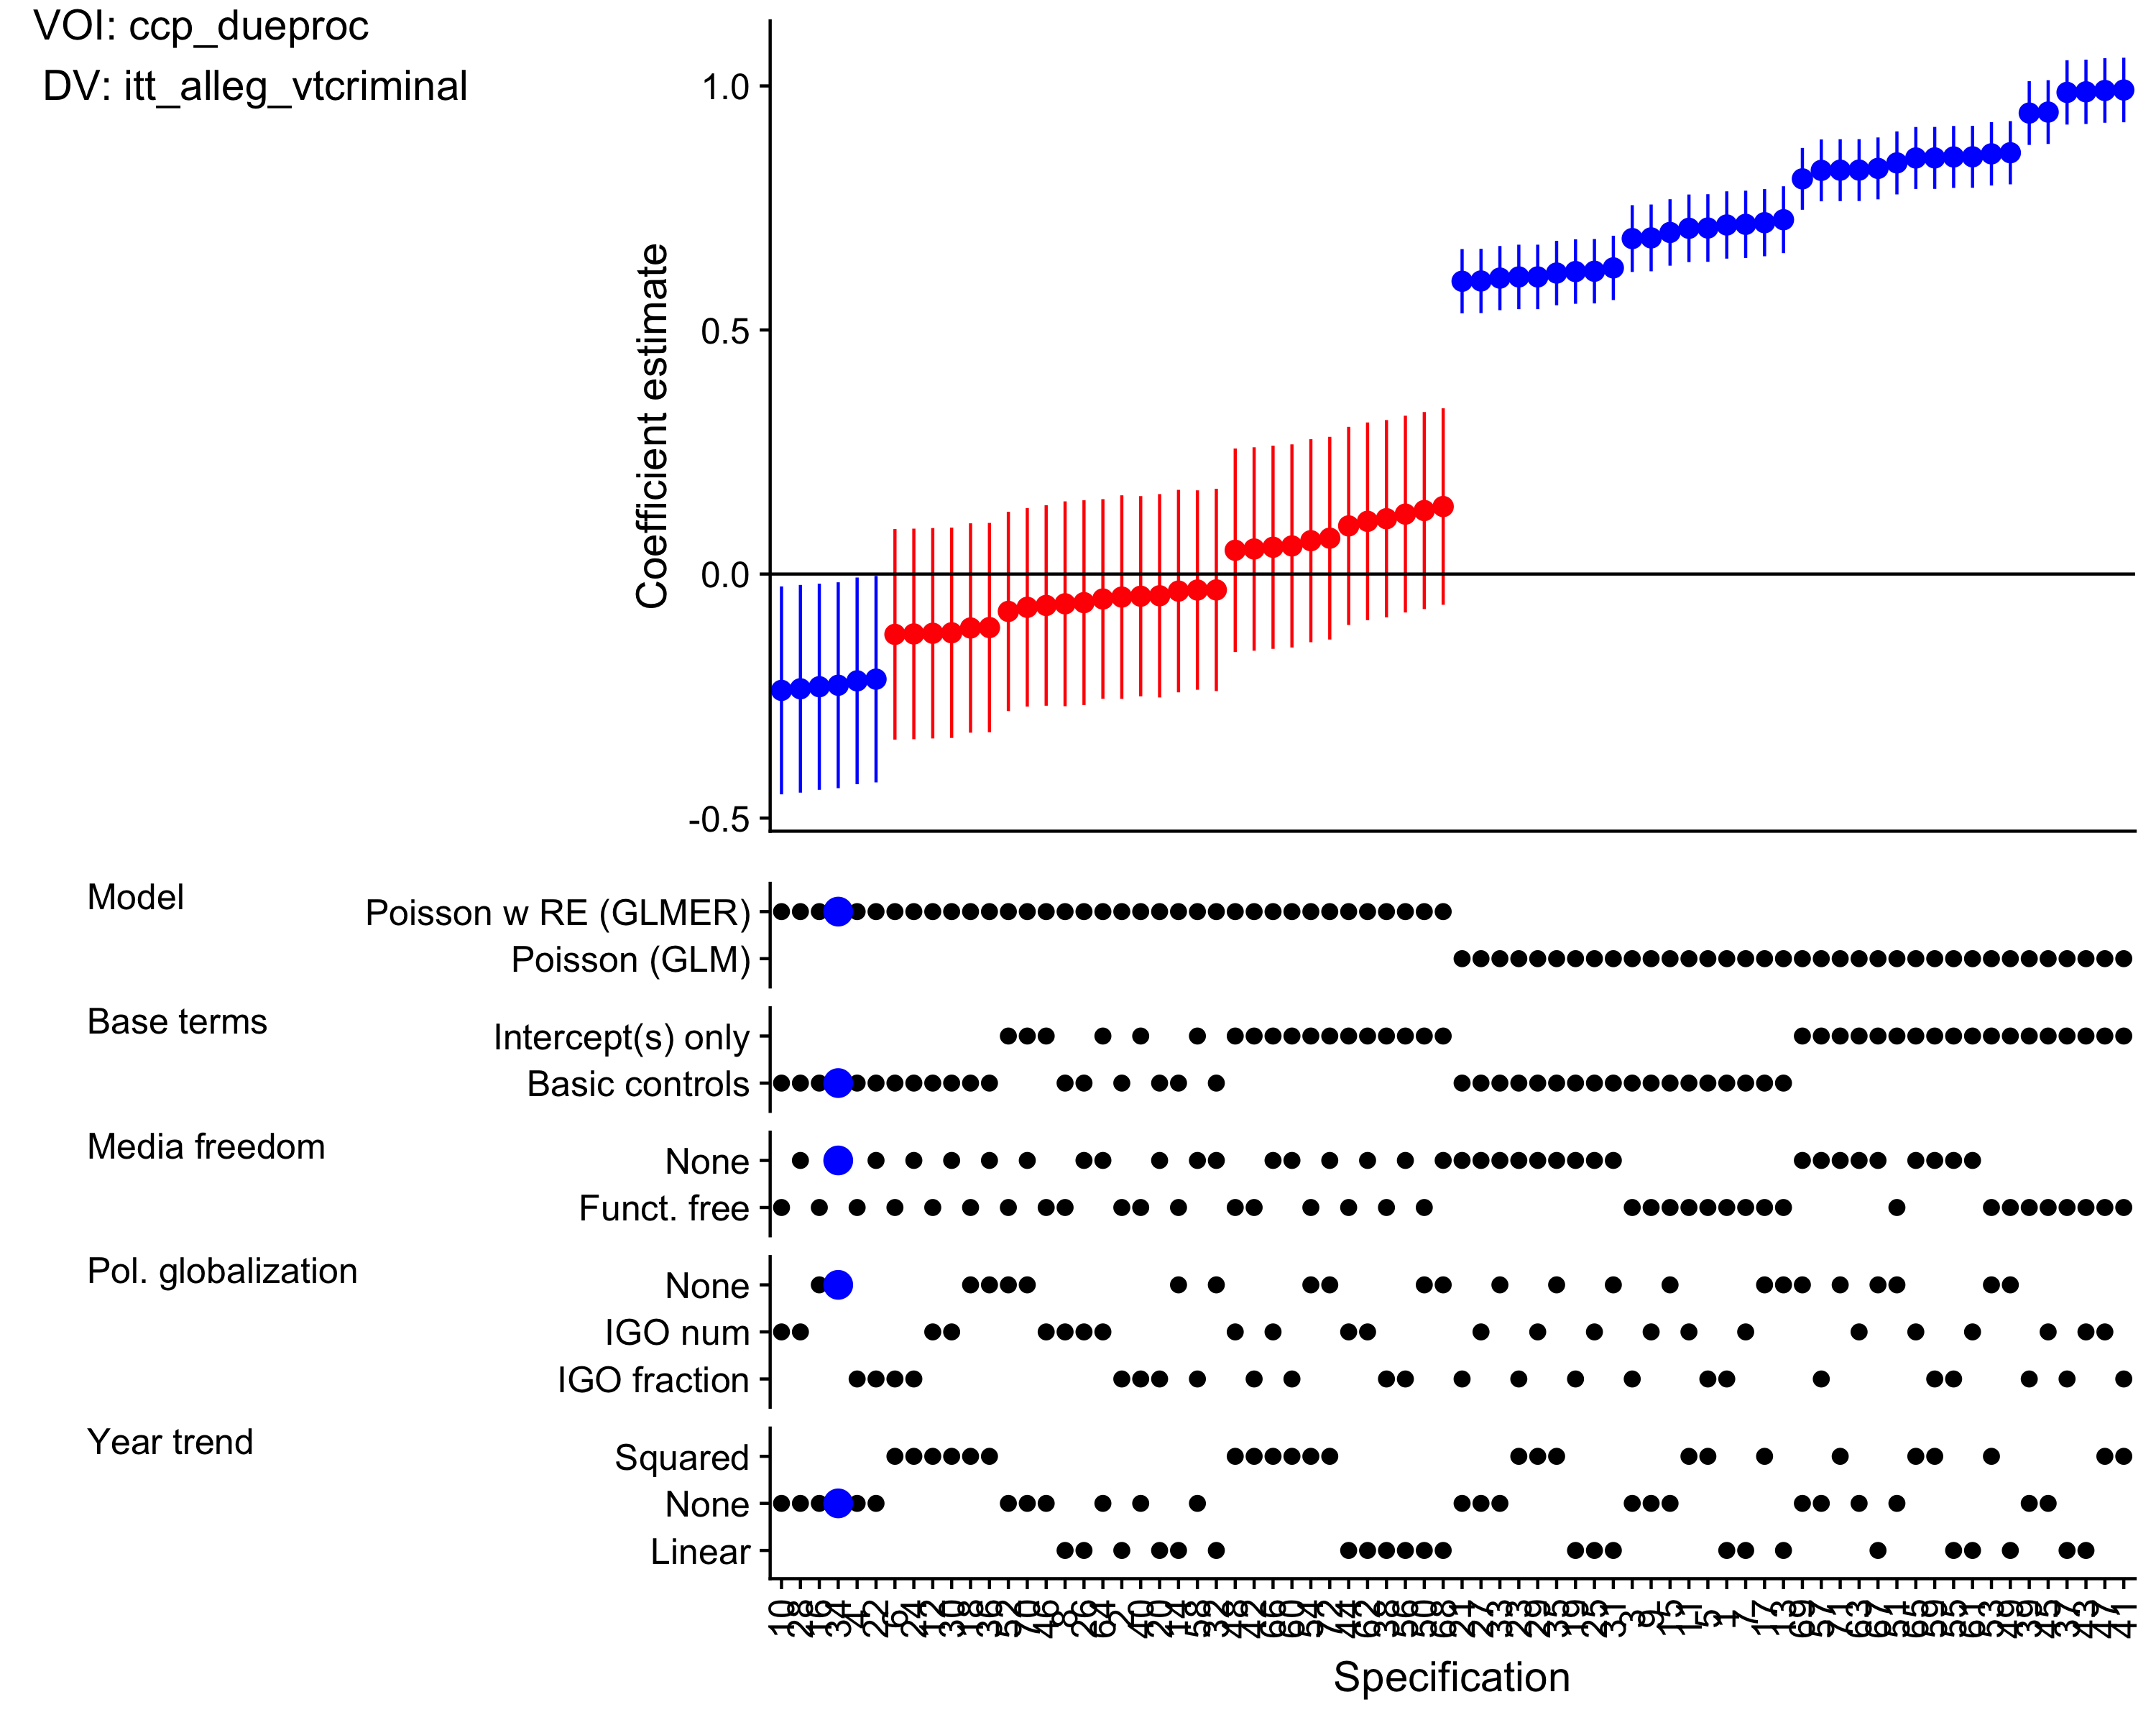
\includegraphics{../output/figures-robustness/specplot-ccp_dueproc-itt_alleg_vtcriminal.png}

The plot consists of two main elements. The panel on the top shows the
coefficient estimates for the variable of interest over a number of
different specification on the x-axis. The points and lines show point
estimates and 95\% confidence intervals; they are colored red and blue
for stastitically significant (\(p\)-value \(< 0.05\)) negative and
positive effects and grey for statisticall insignificant estimates.

The second panel at the bottom shows details for each specification. All
the way on the left are the labels for each specification choice; the
elements from which one could choose are in the next column. For example
for ``Model'' we made a choice between a regular Poisson count model
with global intercept only, versus a GLMER Poisson model that also
includes country random effects (RE). The \(x\)-axis are still
specifications, and the dots in the plot mark what choices were made in
each specification.

The specification we used in the main paper are highlighted in both
blots with the grey rectangles. We've also annotated each plot with text
in the top left that summarizes the number of significant positive or
negative, as well as insignificant, estimates.

In terms of interpretation, we can firstly see that a large but not
overwhelming proportion of estimates are positive and significant. The
patterns of dots in the specification bottom plot can give some hints at
what is driven estimate patterns. Long sequences like that for ``Model''
indicate that a specification choice is strongly related to estimates,
and indeed the positive and significant estimates are entirely due to
using a model with only a global, not country random, intercepts.
Uniform spacing on the other hand indicates that a choice plays only a
small row. This is for example the case with Media freedom when using a
Poisson RE model--the estimates change only slightly as the media
freedom indicator changes.

\hypertarget{list-of-all-specification-plots-by-voi}{%
\subsection{List of all specification plots, by
VOI}\label{list-of-all-specification-plots-by-voi}}

\hypertarget{voi-ccp_dueproc}{%
\subsection{VOI: ccp\_dueproc}\label{voi-ccp_dueproc}}

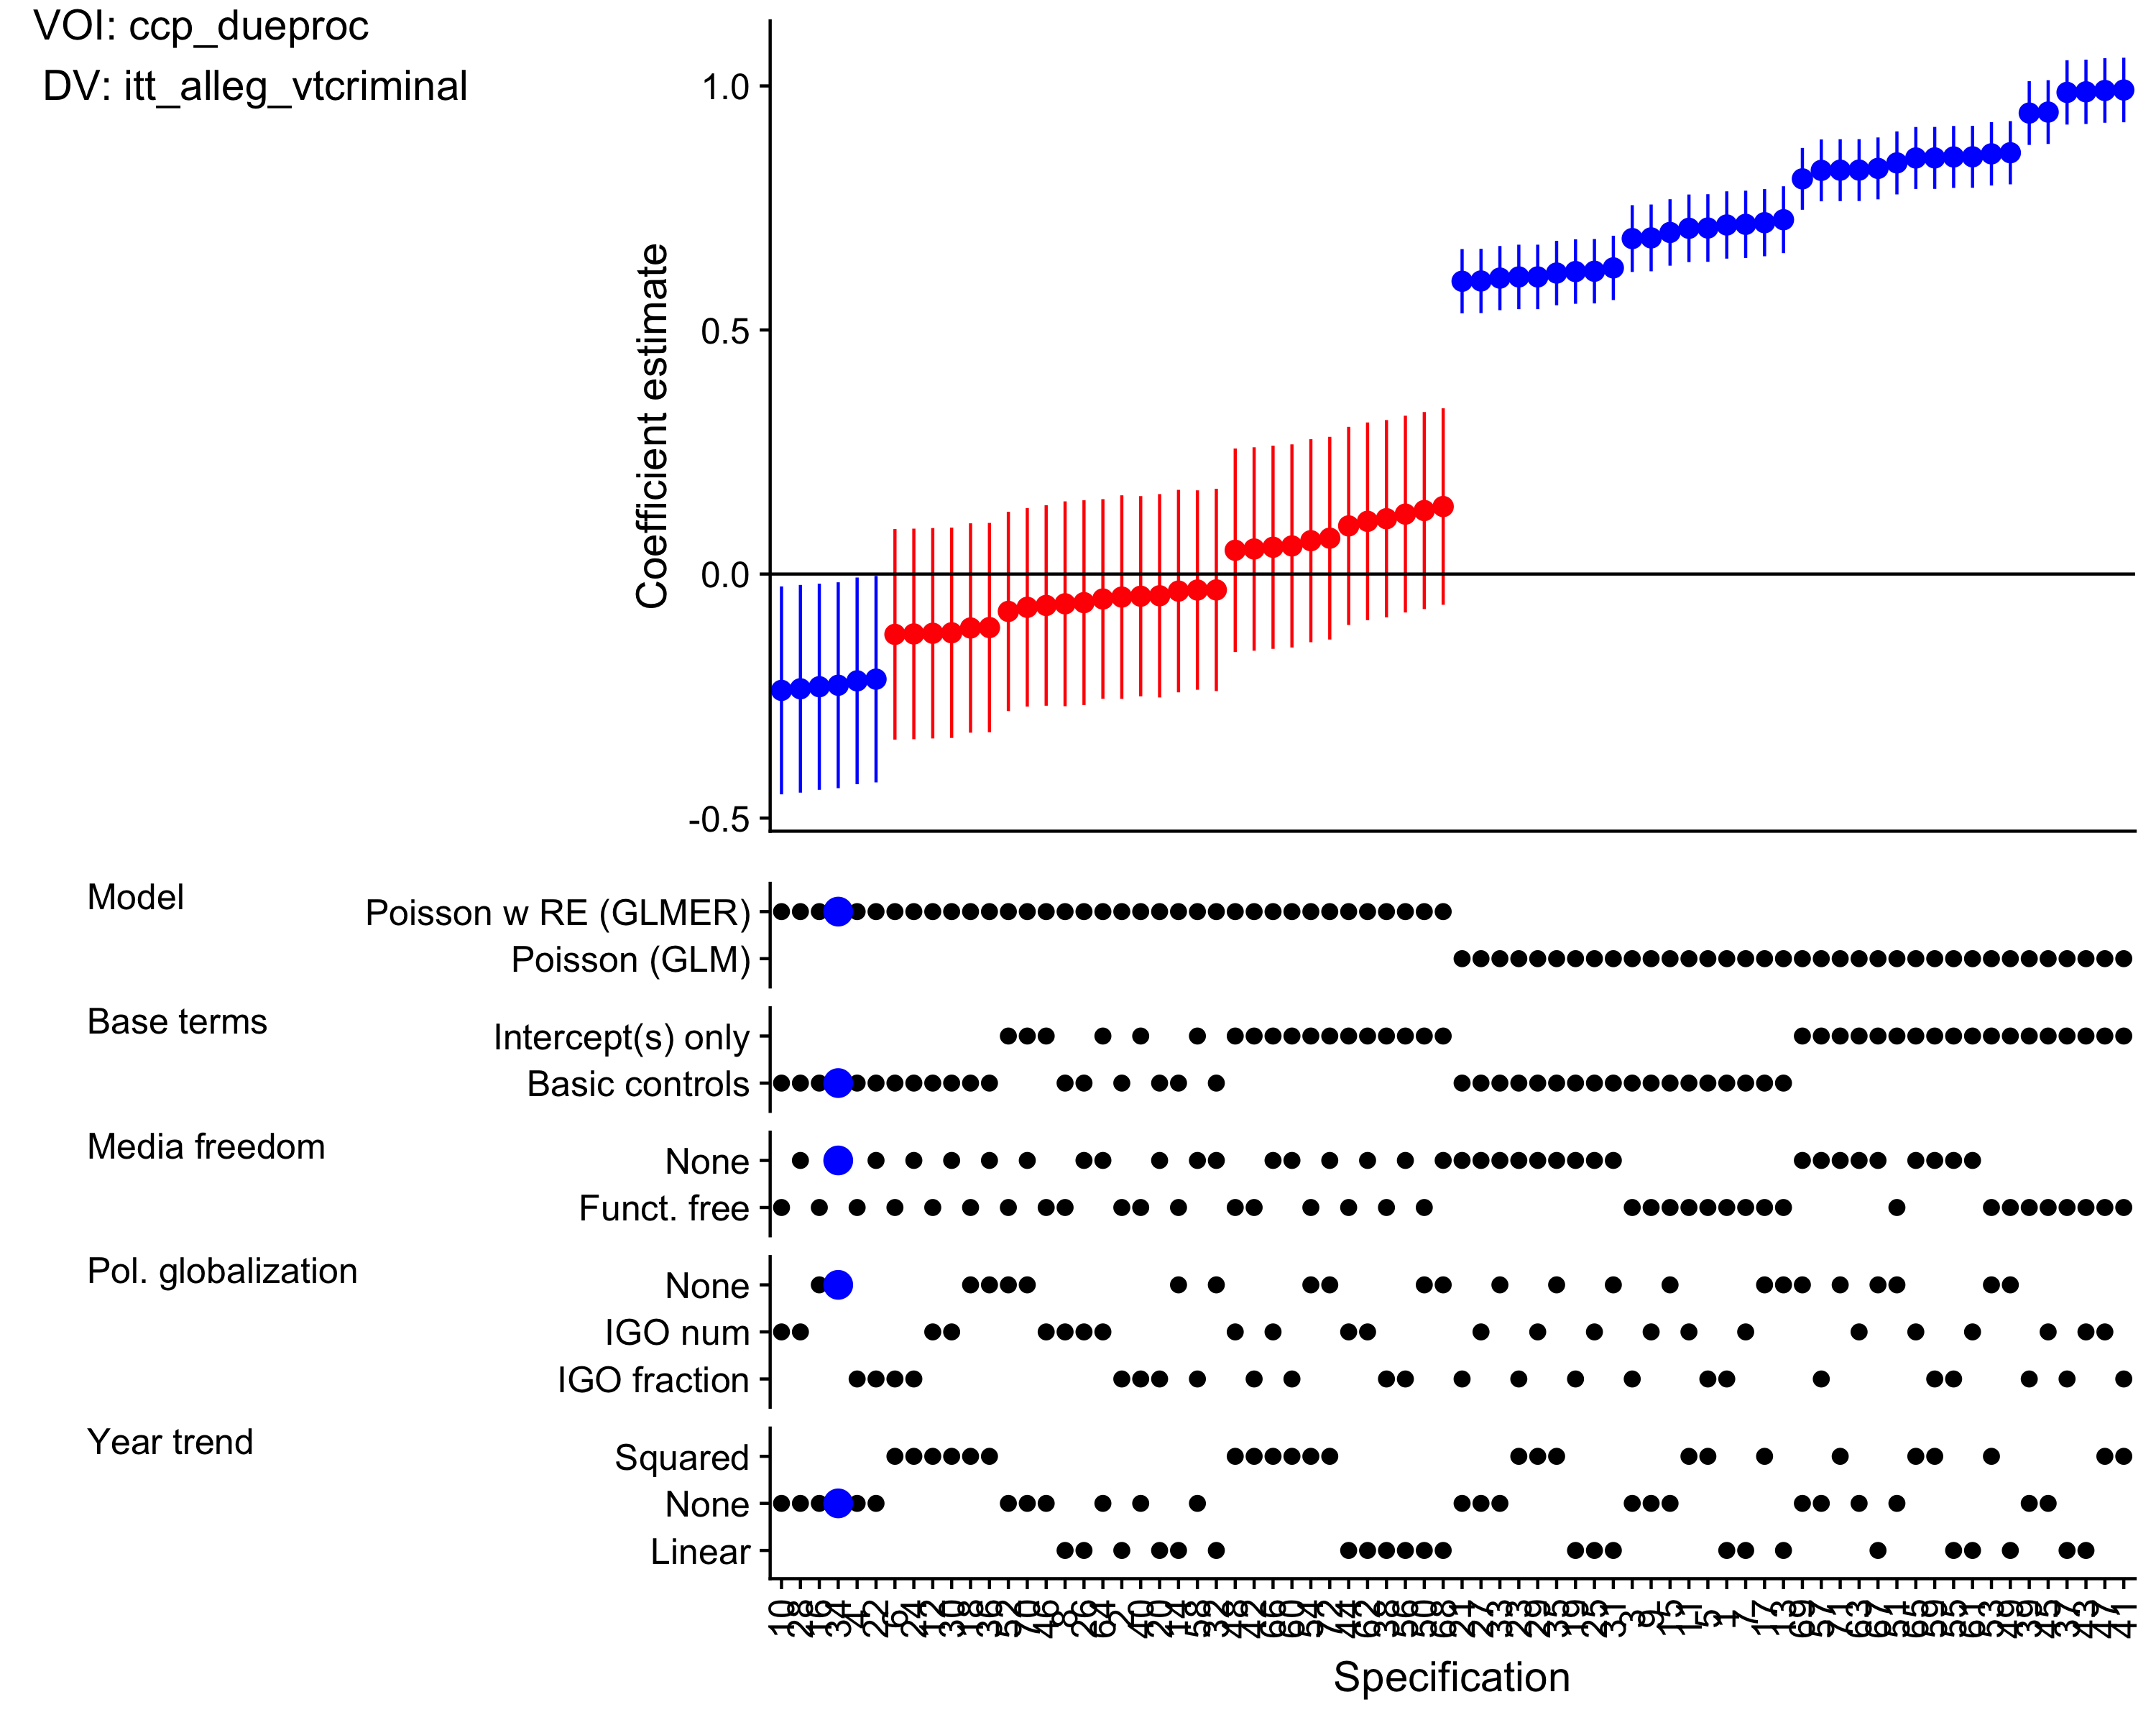
\includegraphics[height=4in]{../output/figures-robustness/specplot-ccp_dueproc-itt_alleg_vtcriminal.png}

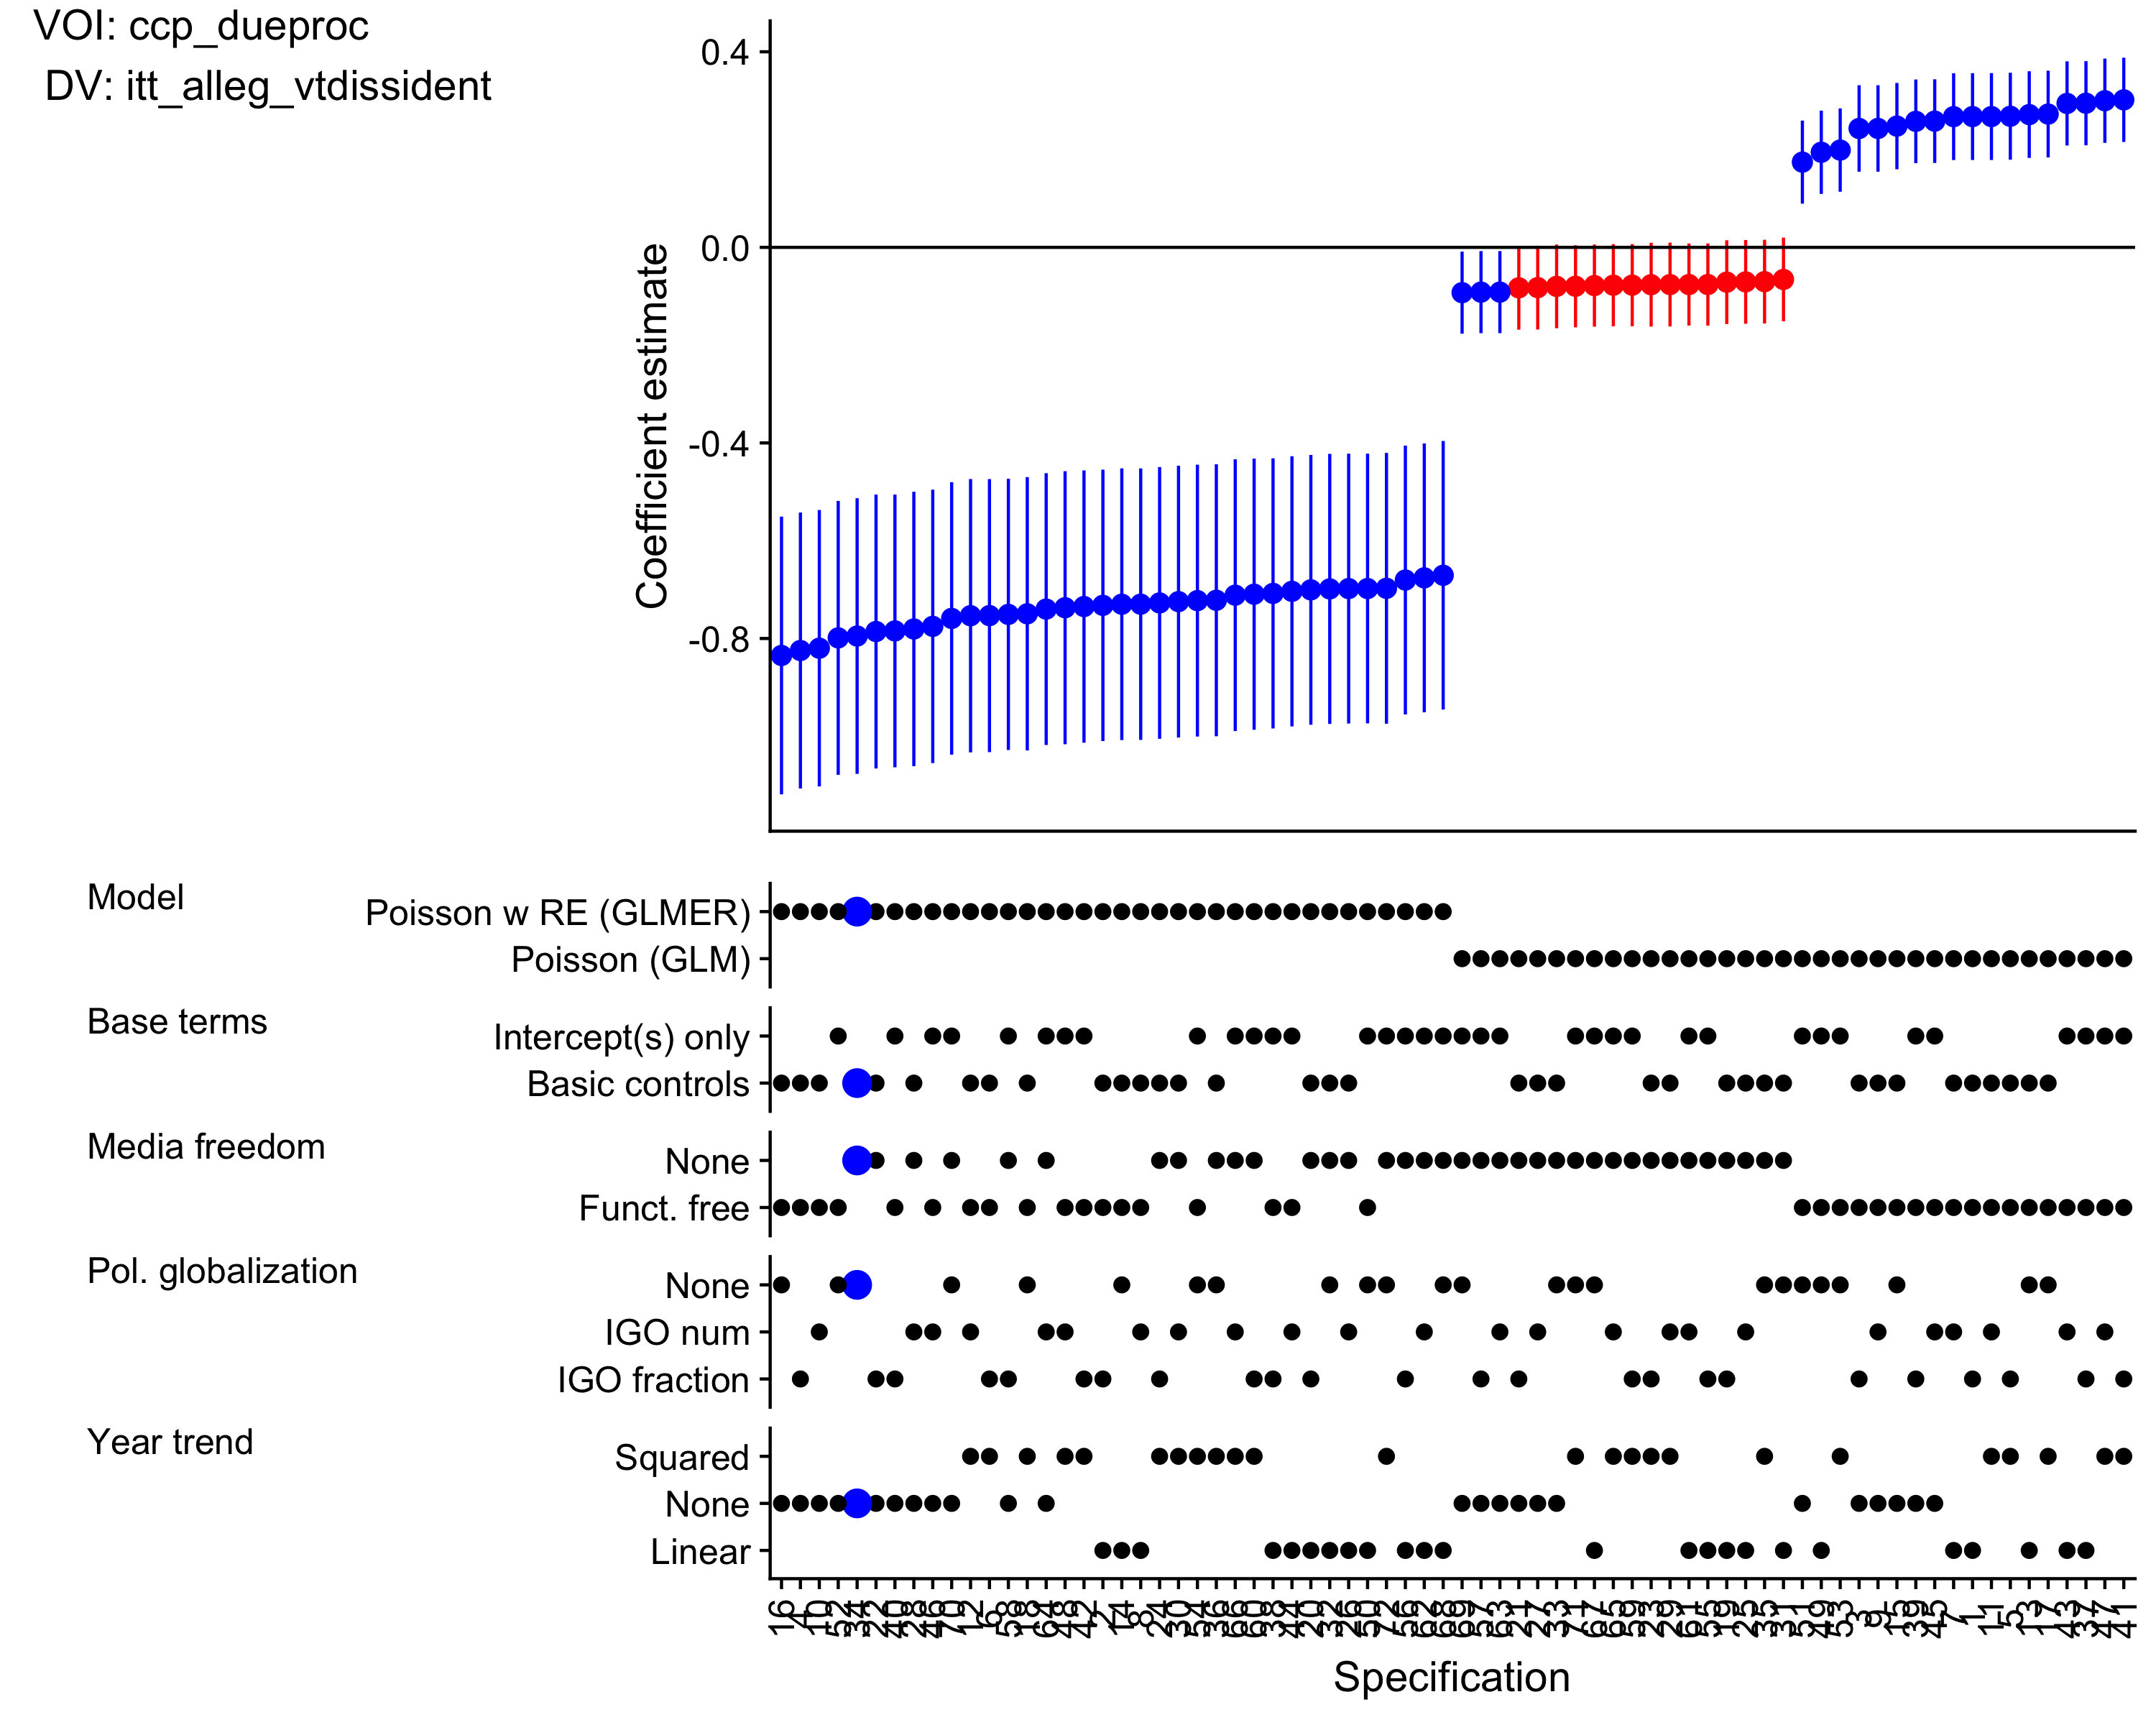
\includegraphics[height=4in]{../output/figures-robustness/specplot-ccp_dueproc-itt_alleg_vtdissident.png}

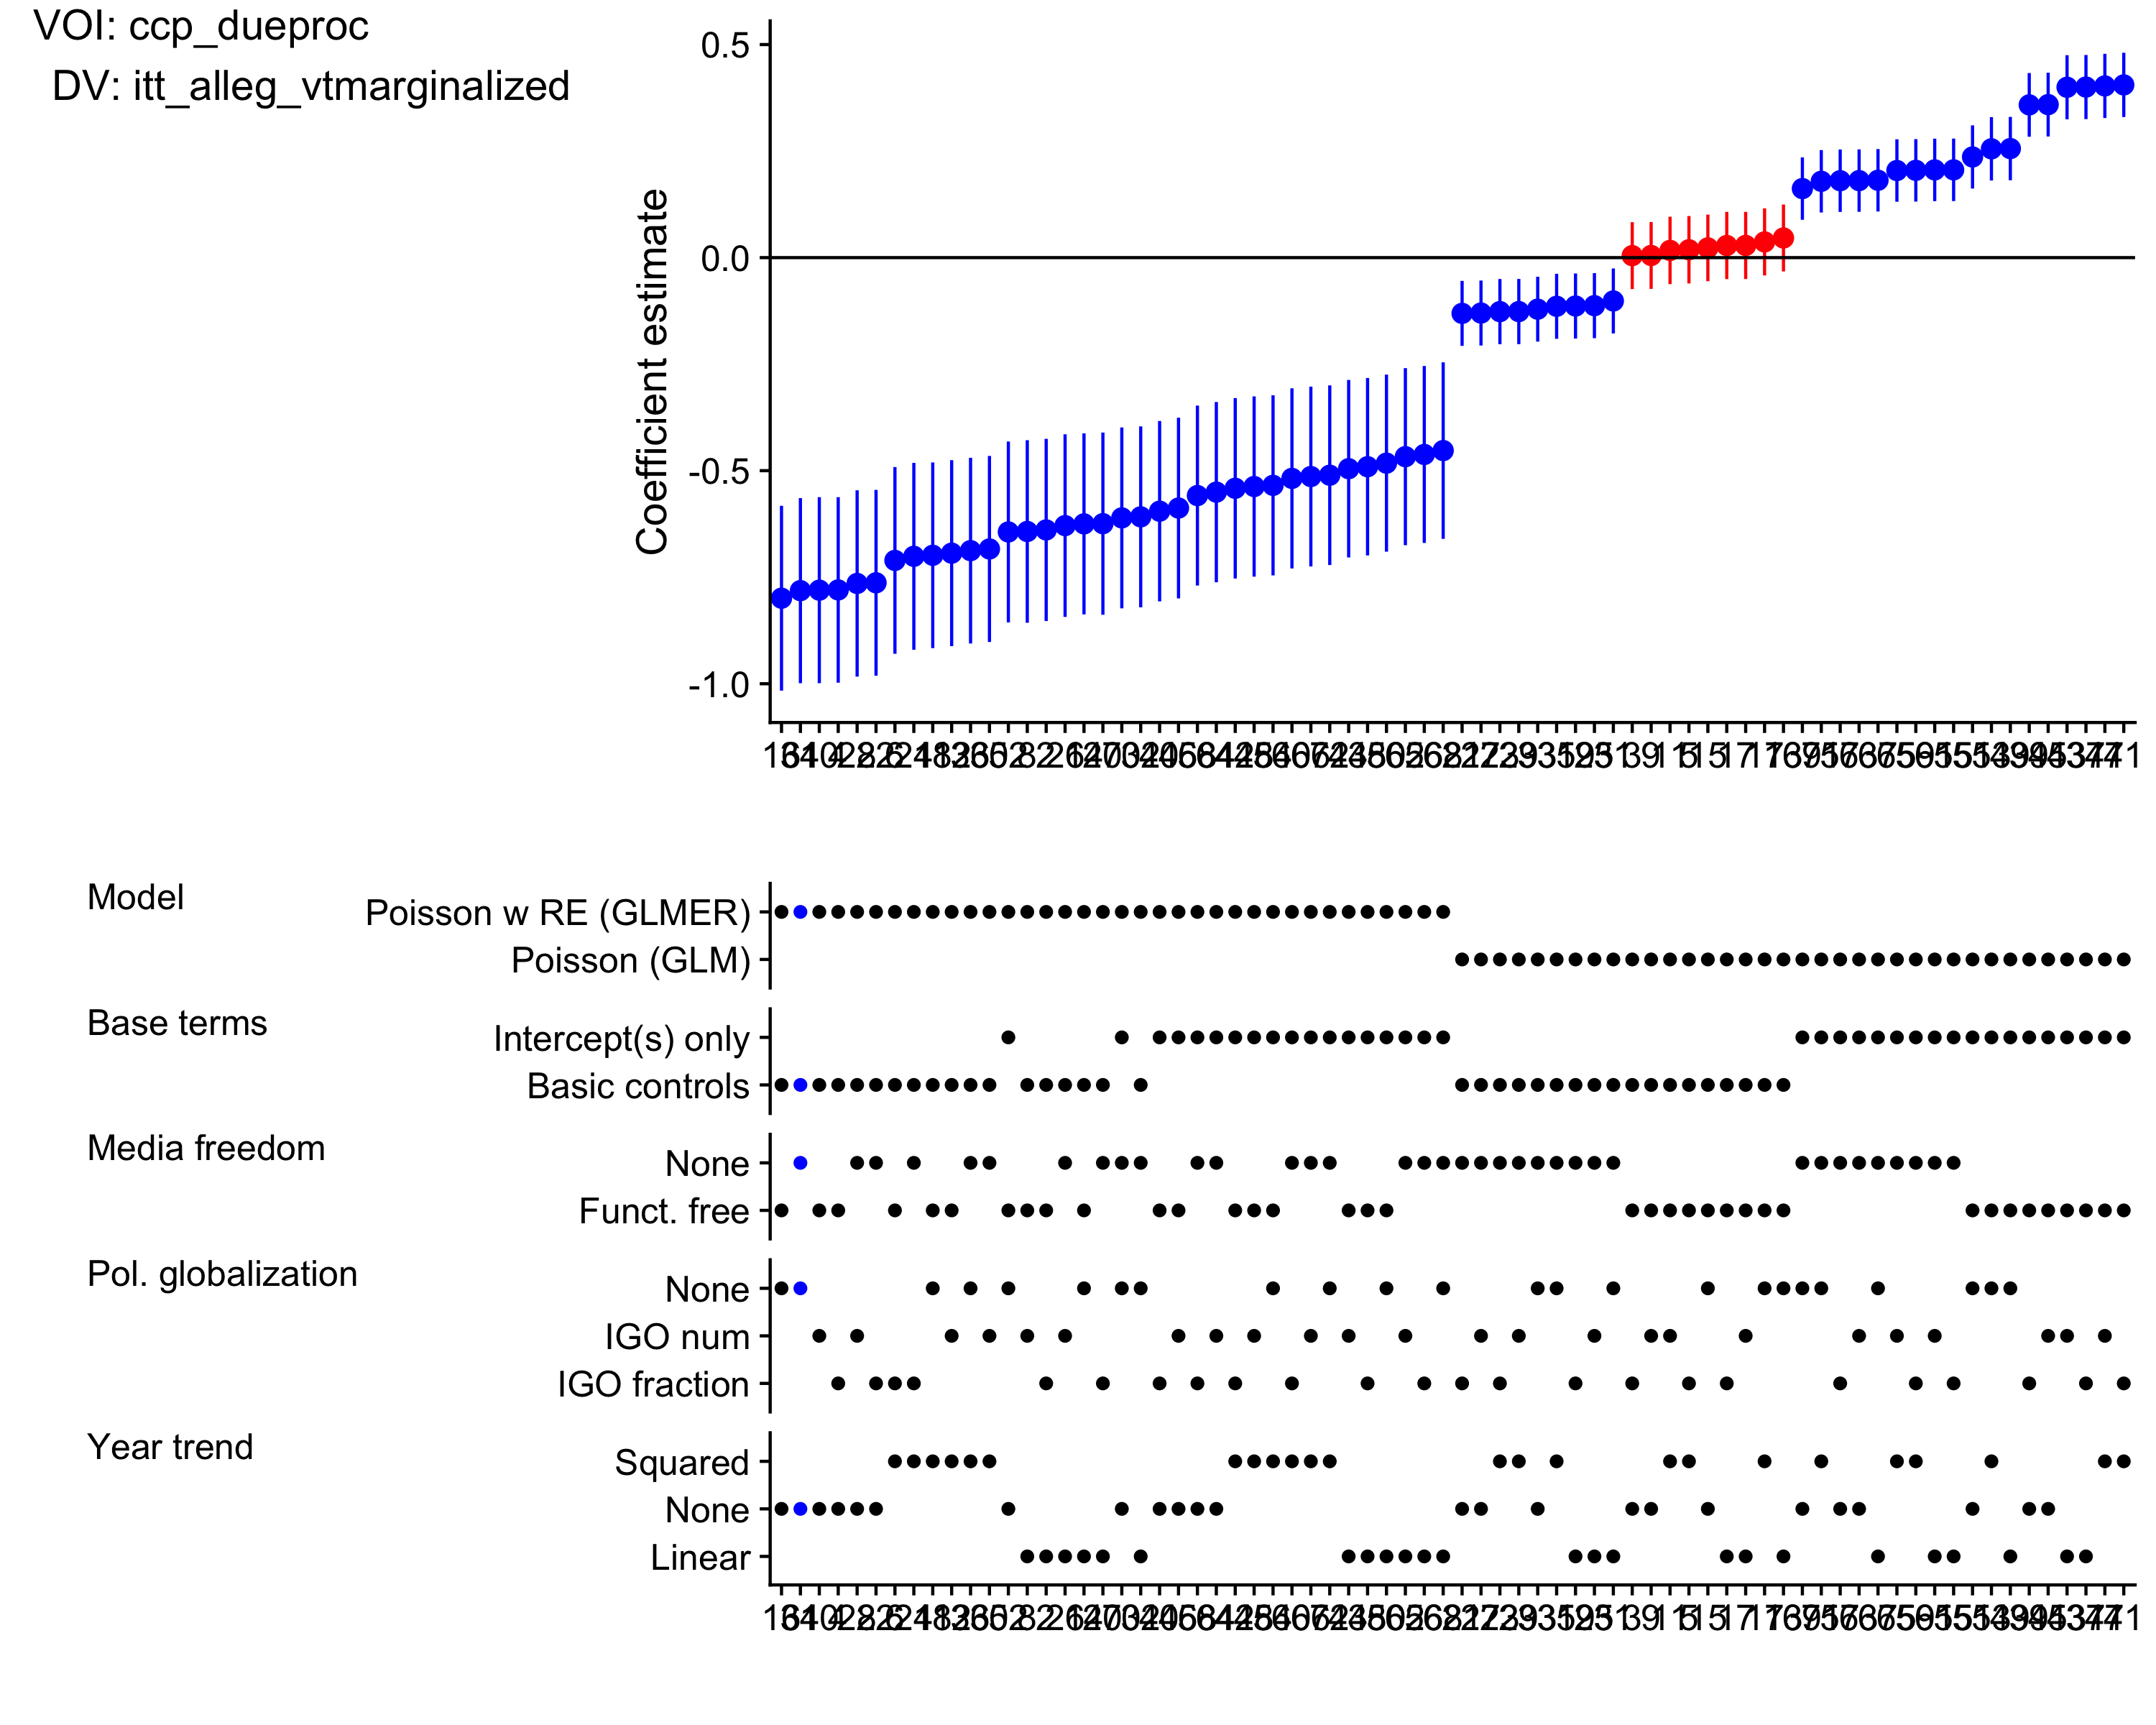
\includegraphics[height=4in]{../output/figures-robustness/specplot-ccp_dueproc-itt_alleg_vtmarginalized.png}

\hypertarget{voi-ccp_habcorp}{%
\subsection{VOI: ccp\_habcorp}\label{voi-ccp_habcorp}}

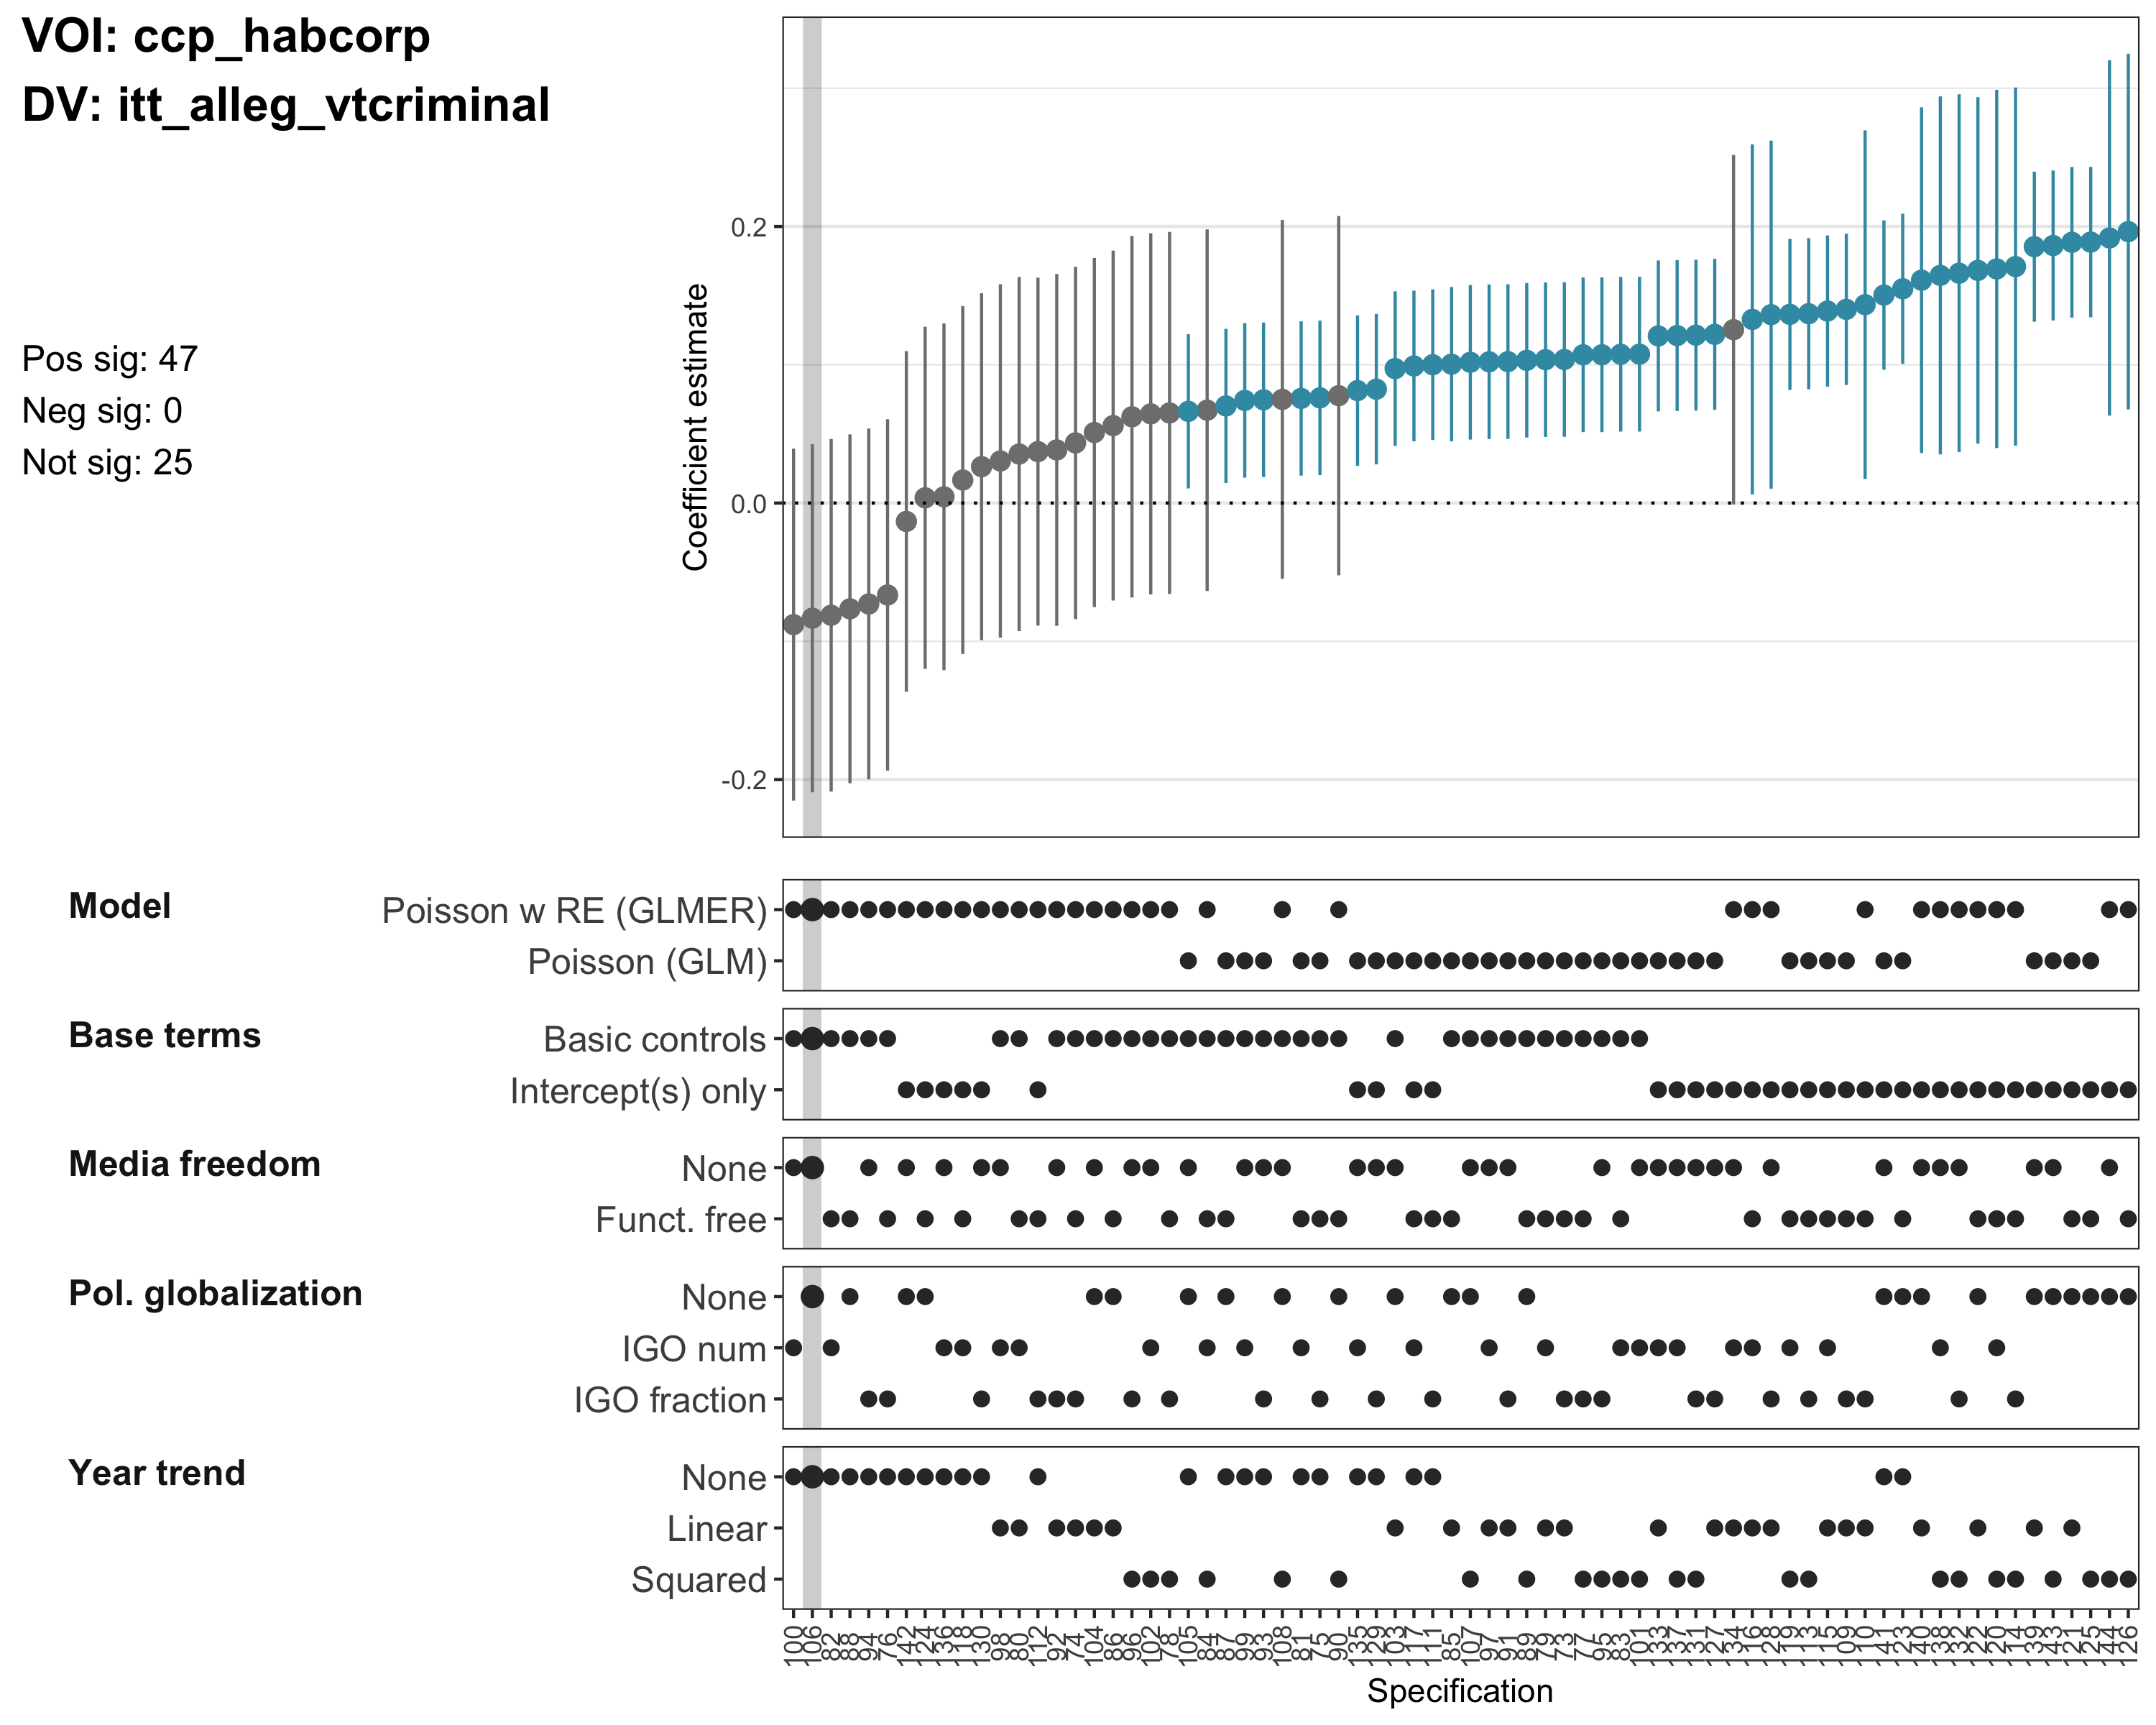
\includegraphics[height=4in]{../output/figures-robustness/specplot-ccp_habcorp-itt_alleg_vtcriminal.png}

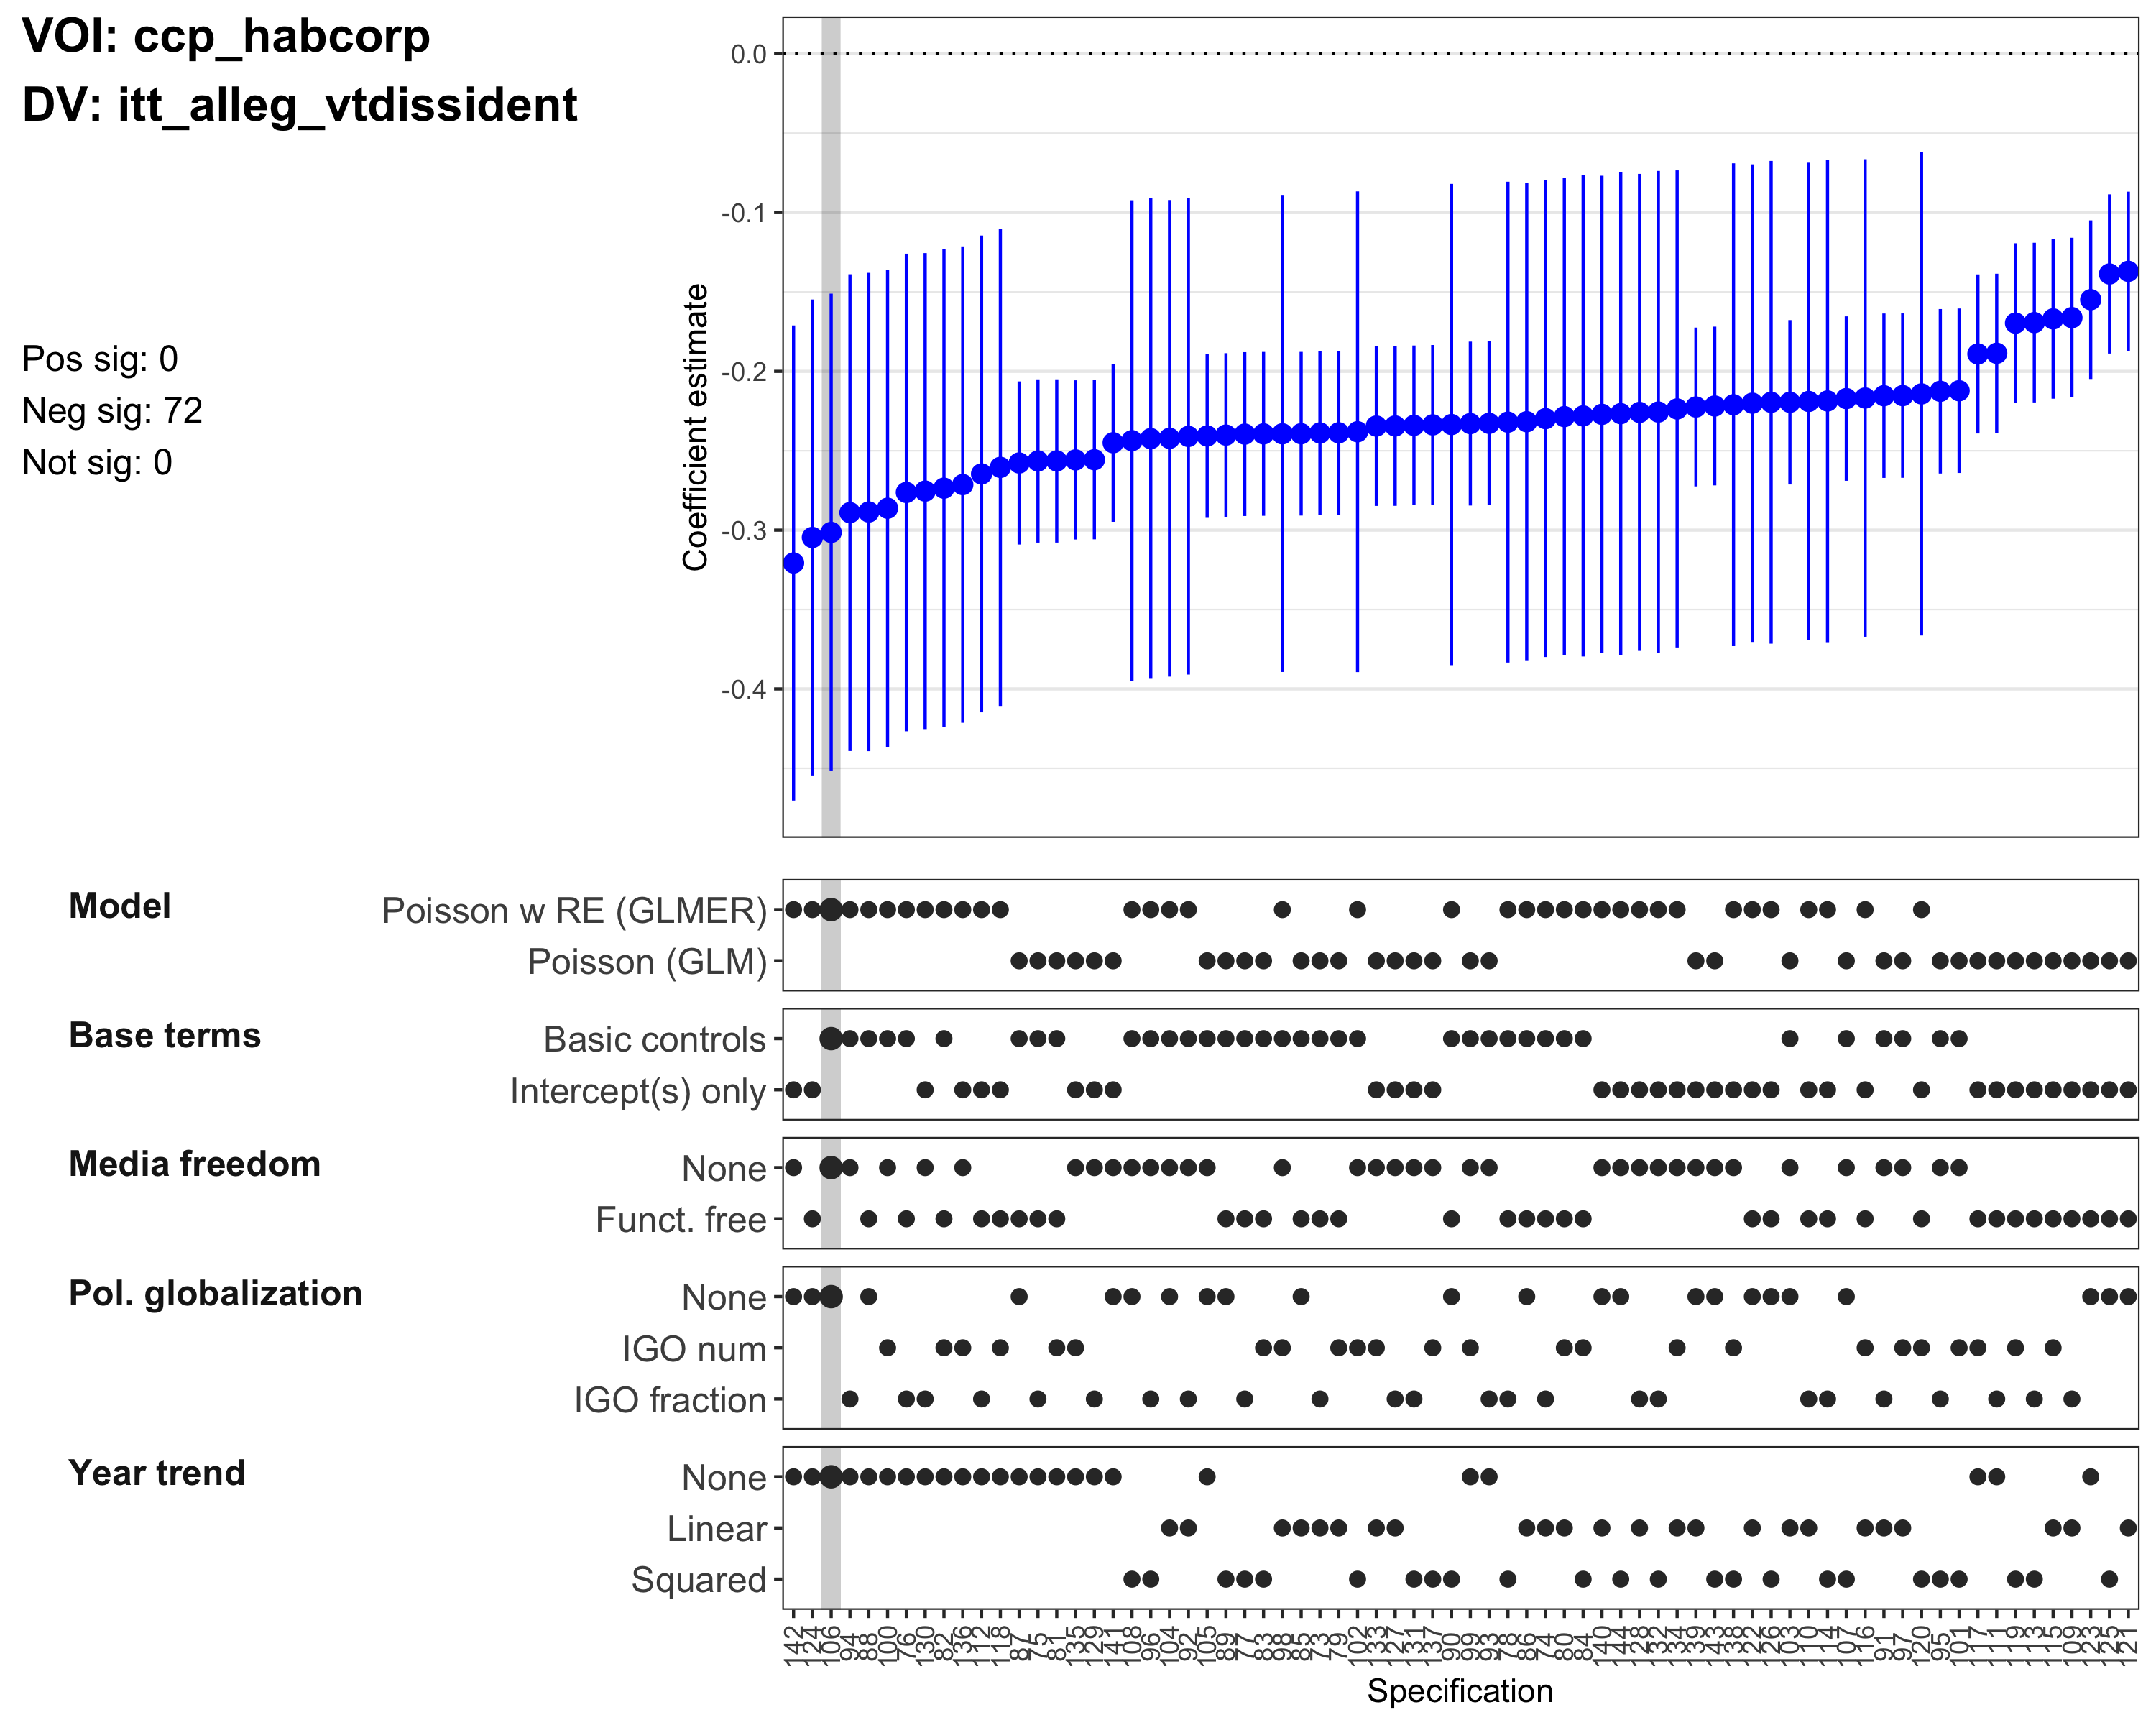
\includegraphics[height=4in]{../output/figures-robustness/specplot-ccp_habcorp-itt_alleg_vtdissident.png}

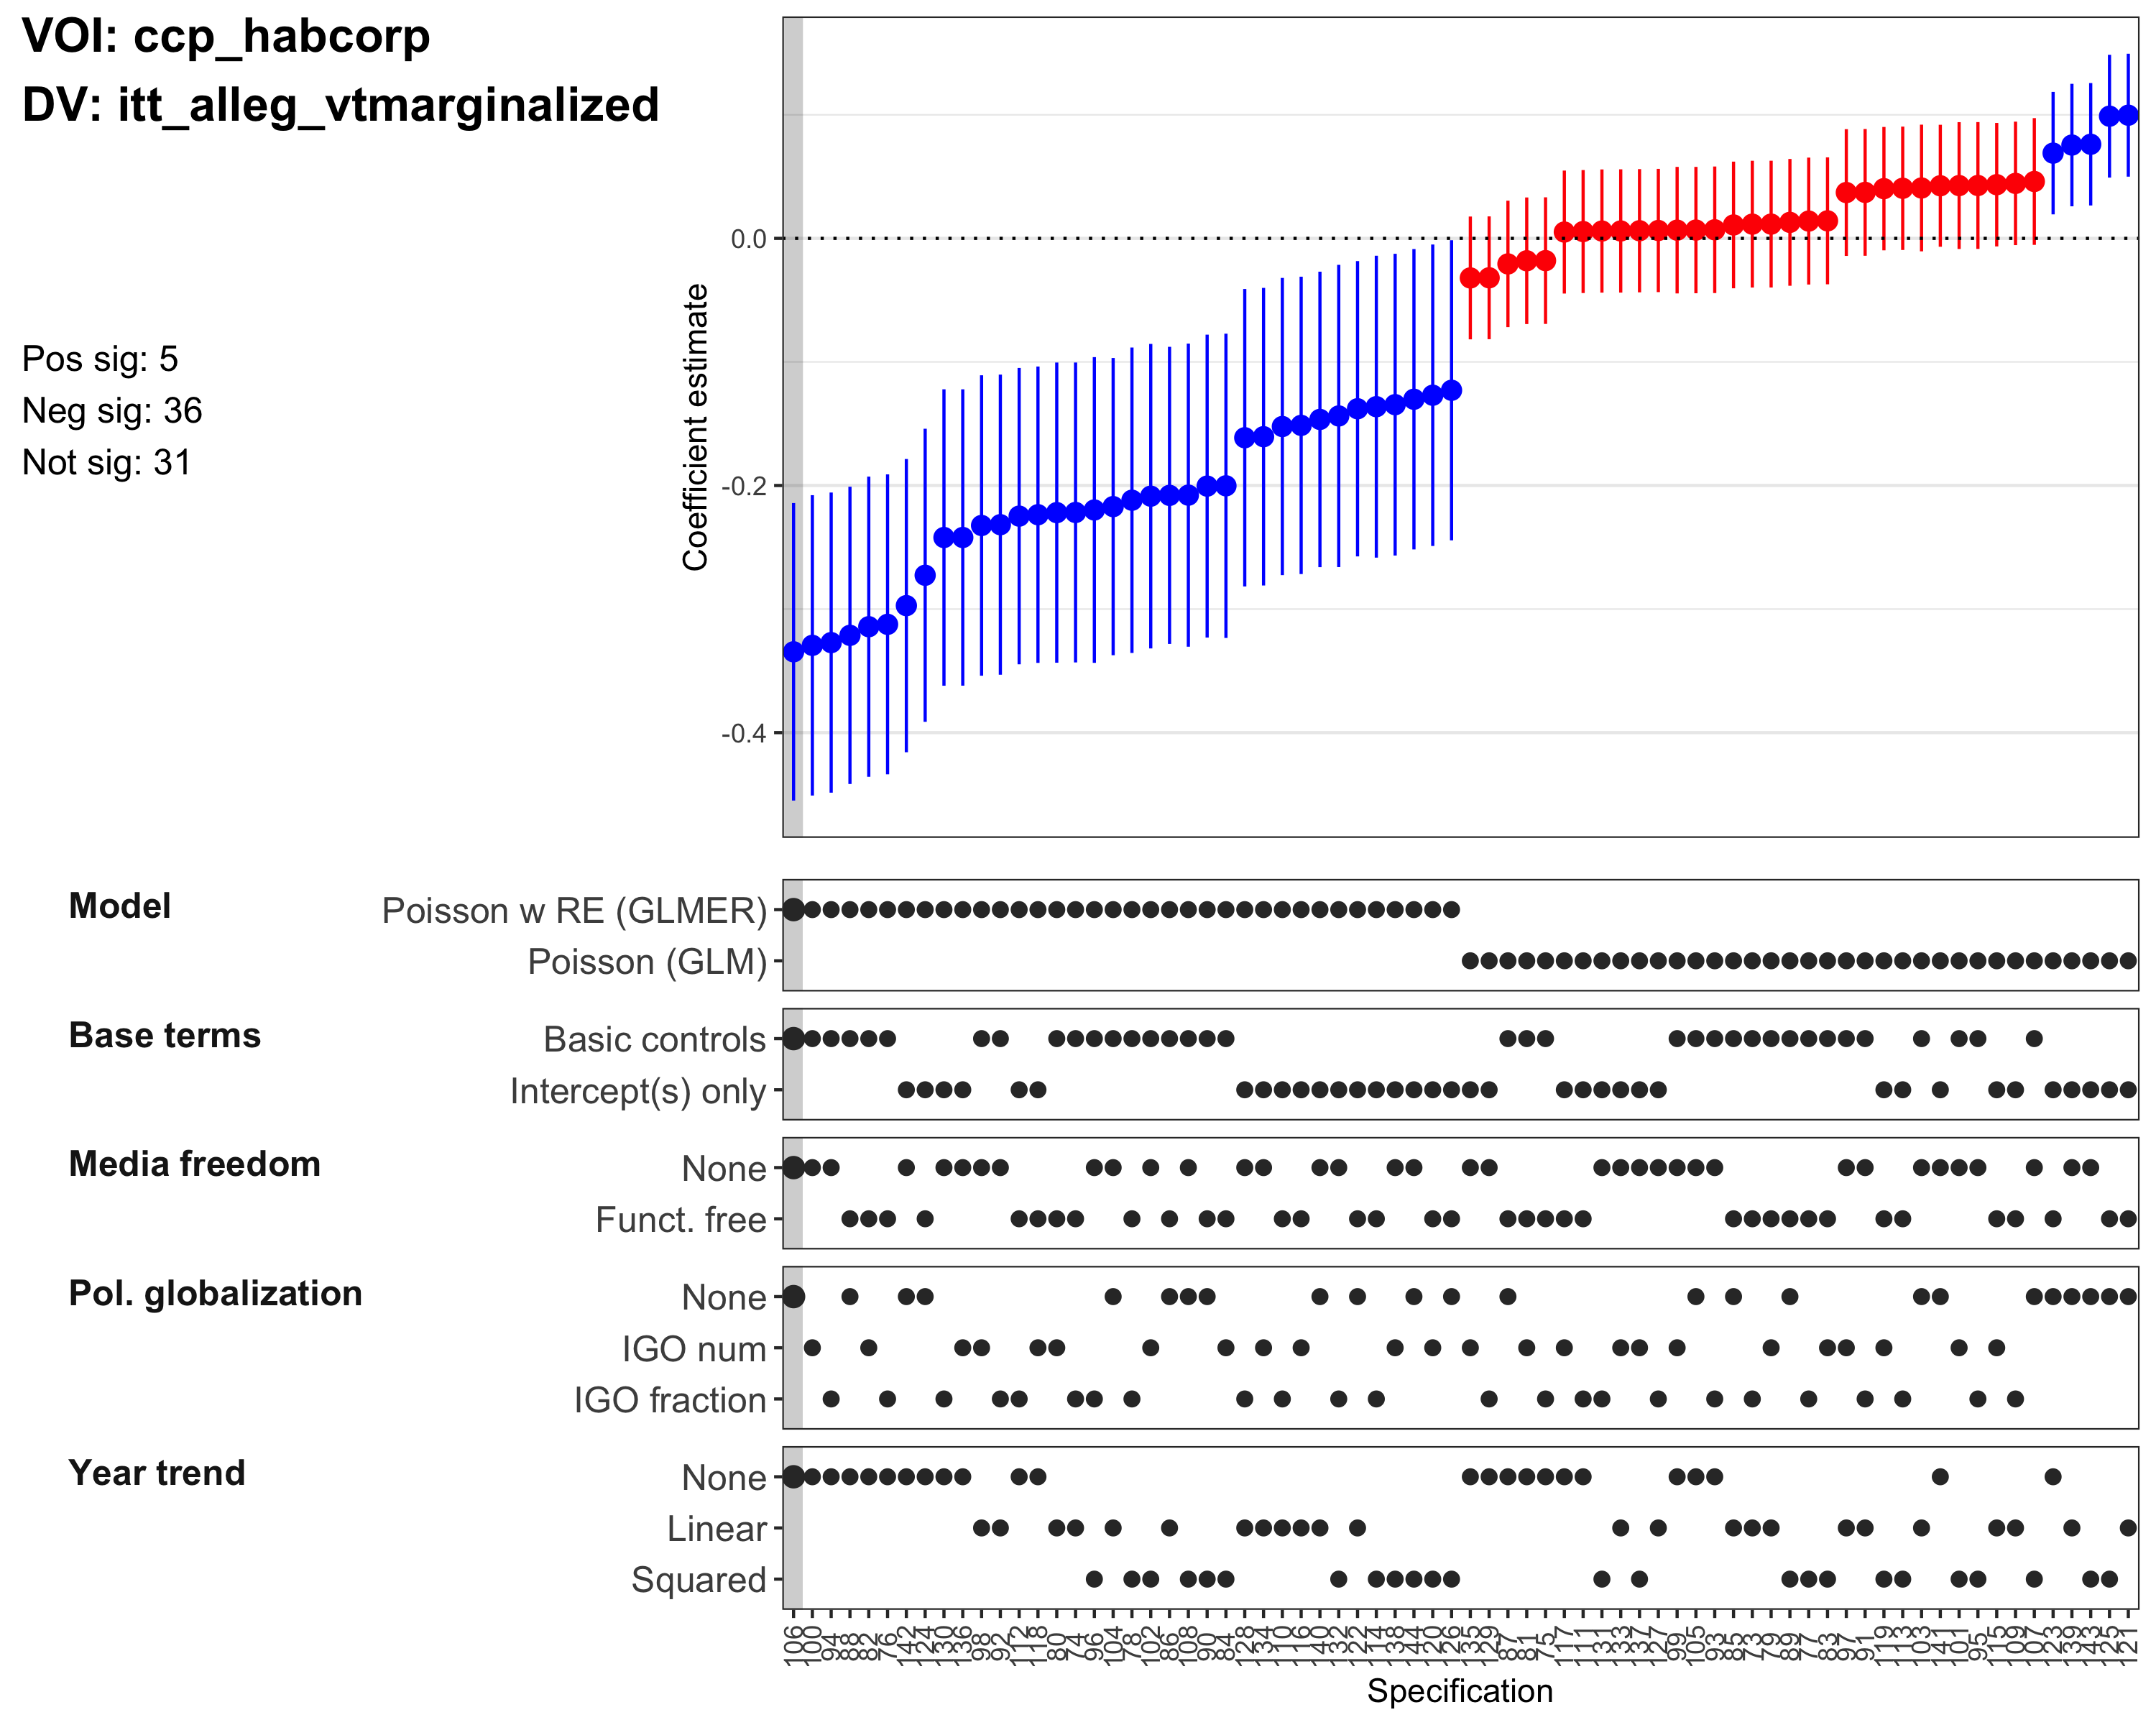
\includegraphics[height=4in]{../output/figures-robustness/specplot-ccp_habcorp-itt_alleg_vtmarginalized.png}

\hypertarget{voi-ccp_prerel}{%
\subsection{VOI: ccp\_prerel}\label{voi-ccp_prerel}}

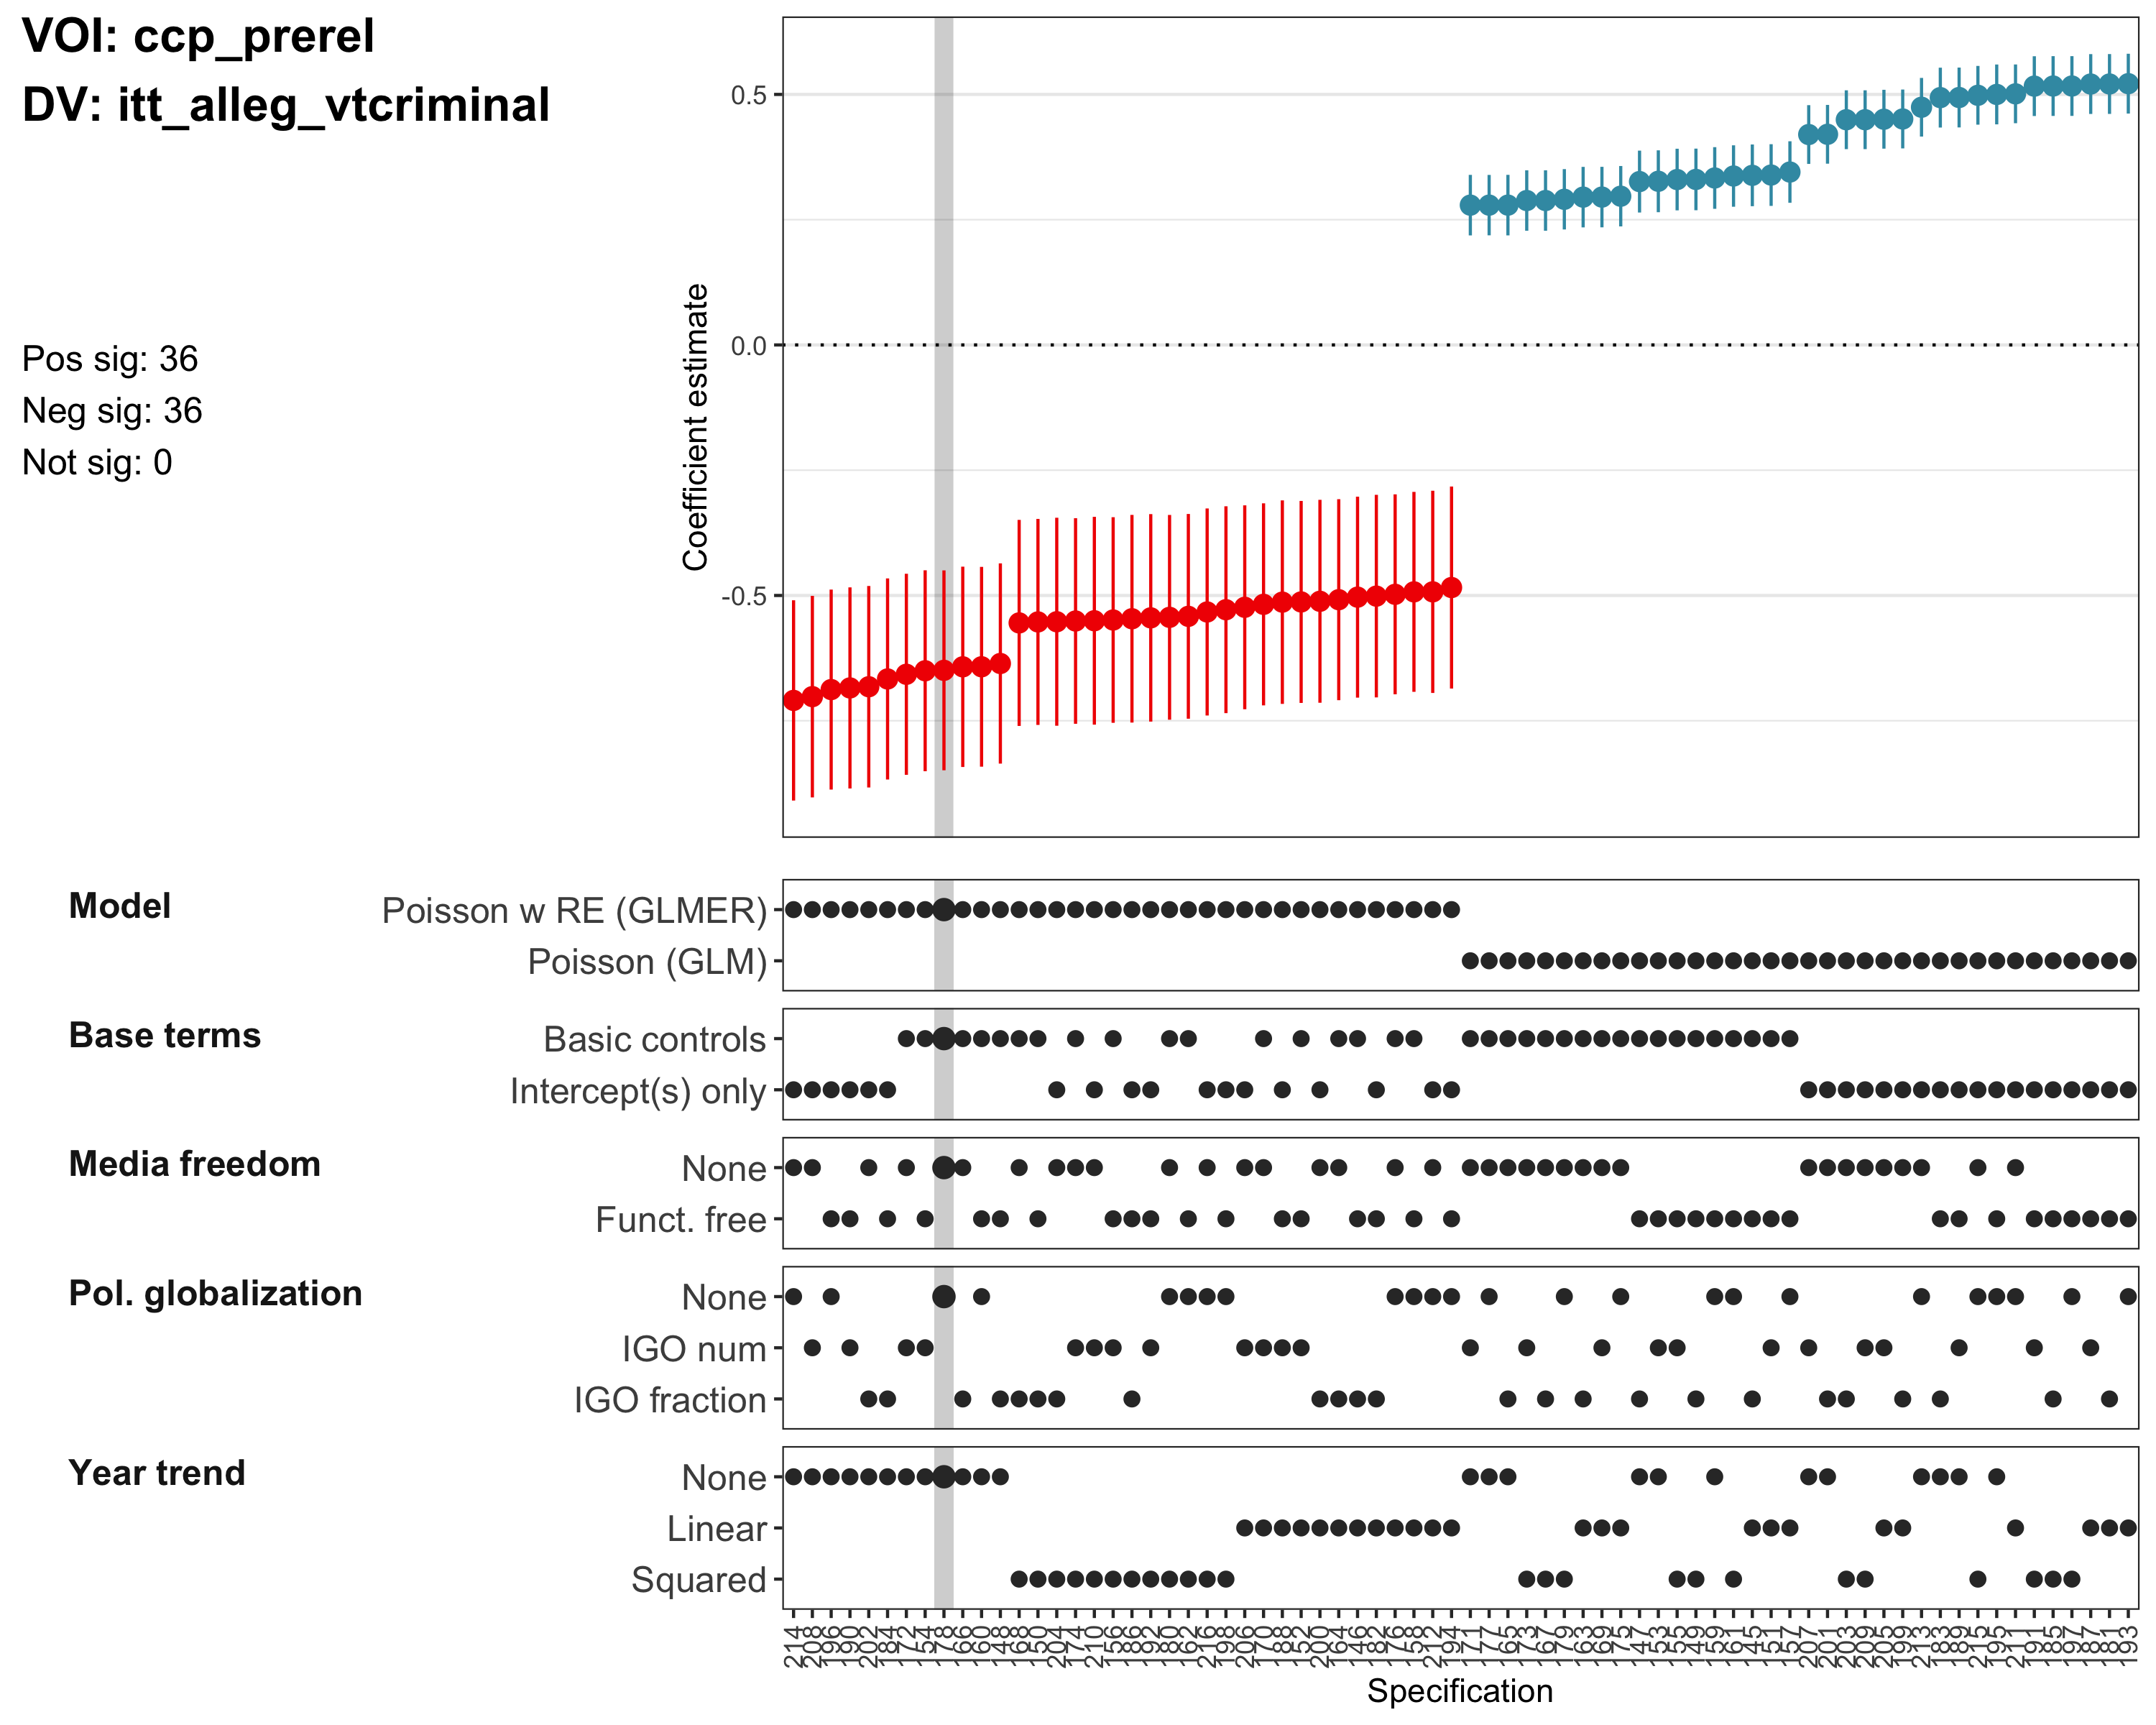
\includegraphics[height=4in]{../output/figures-robustness/specplot-ccp_prerel-itt_alleg_vtcriminal.png}

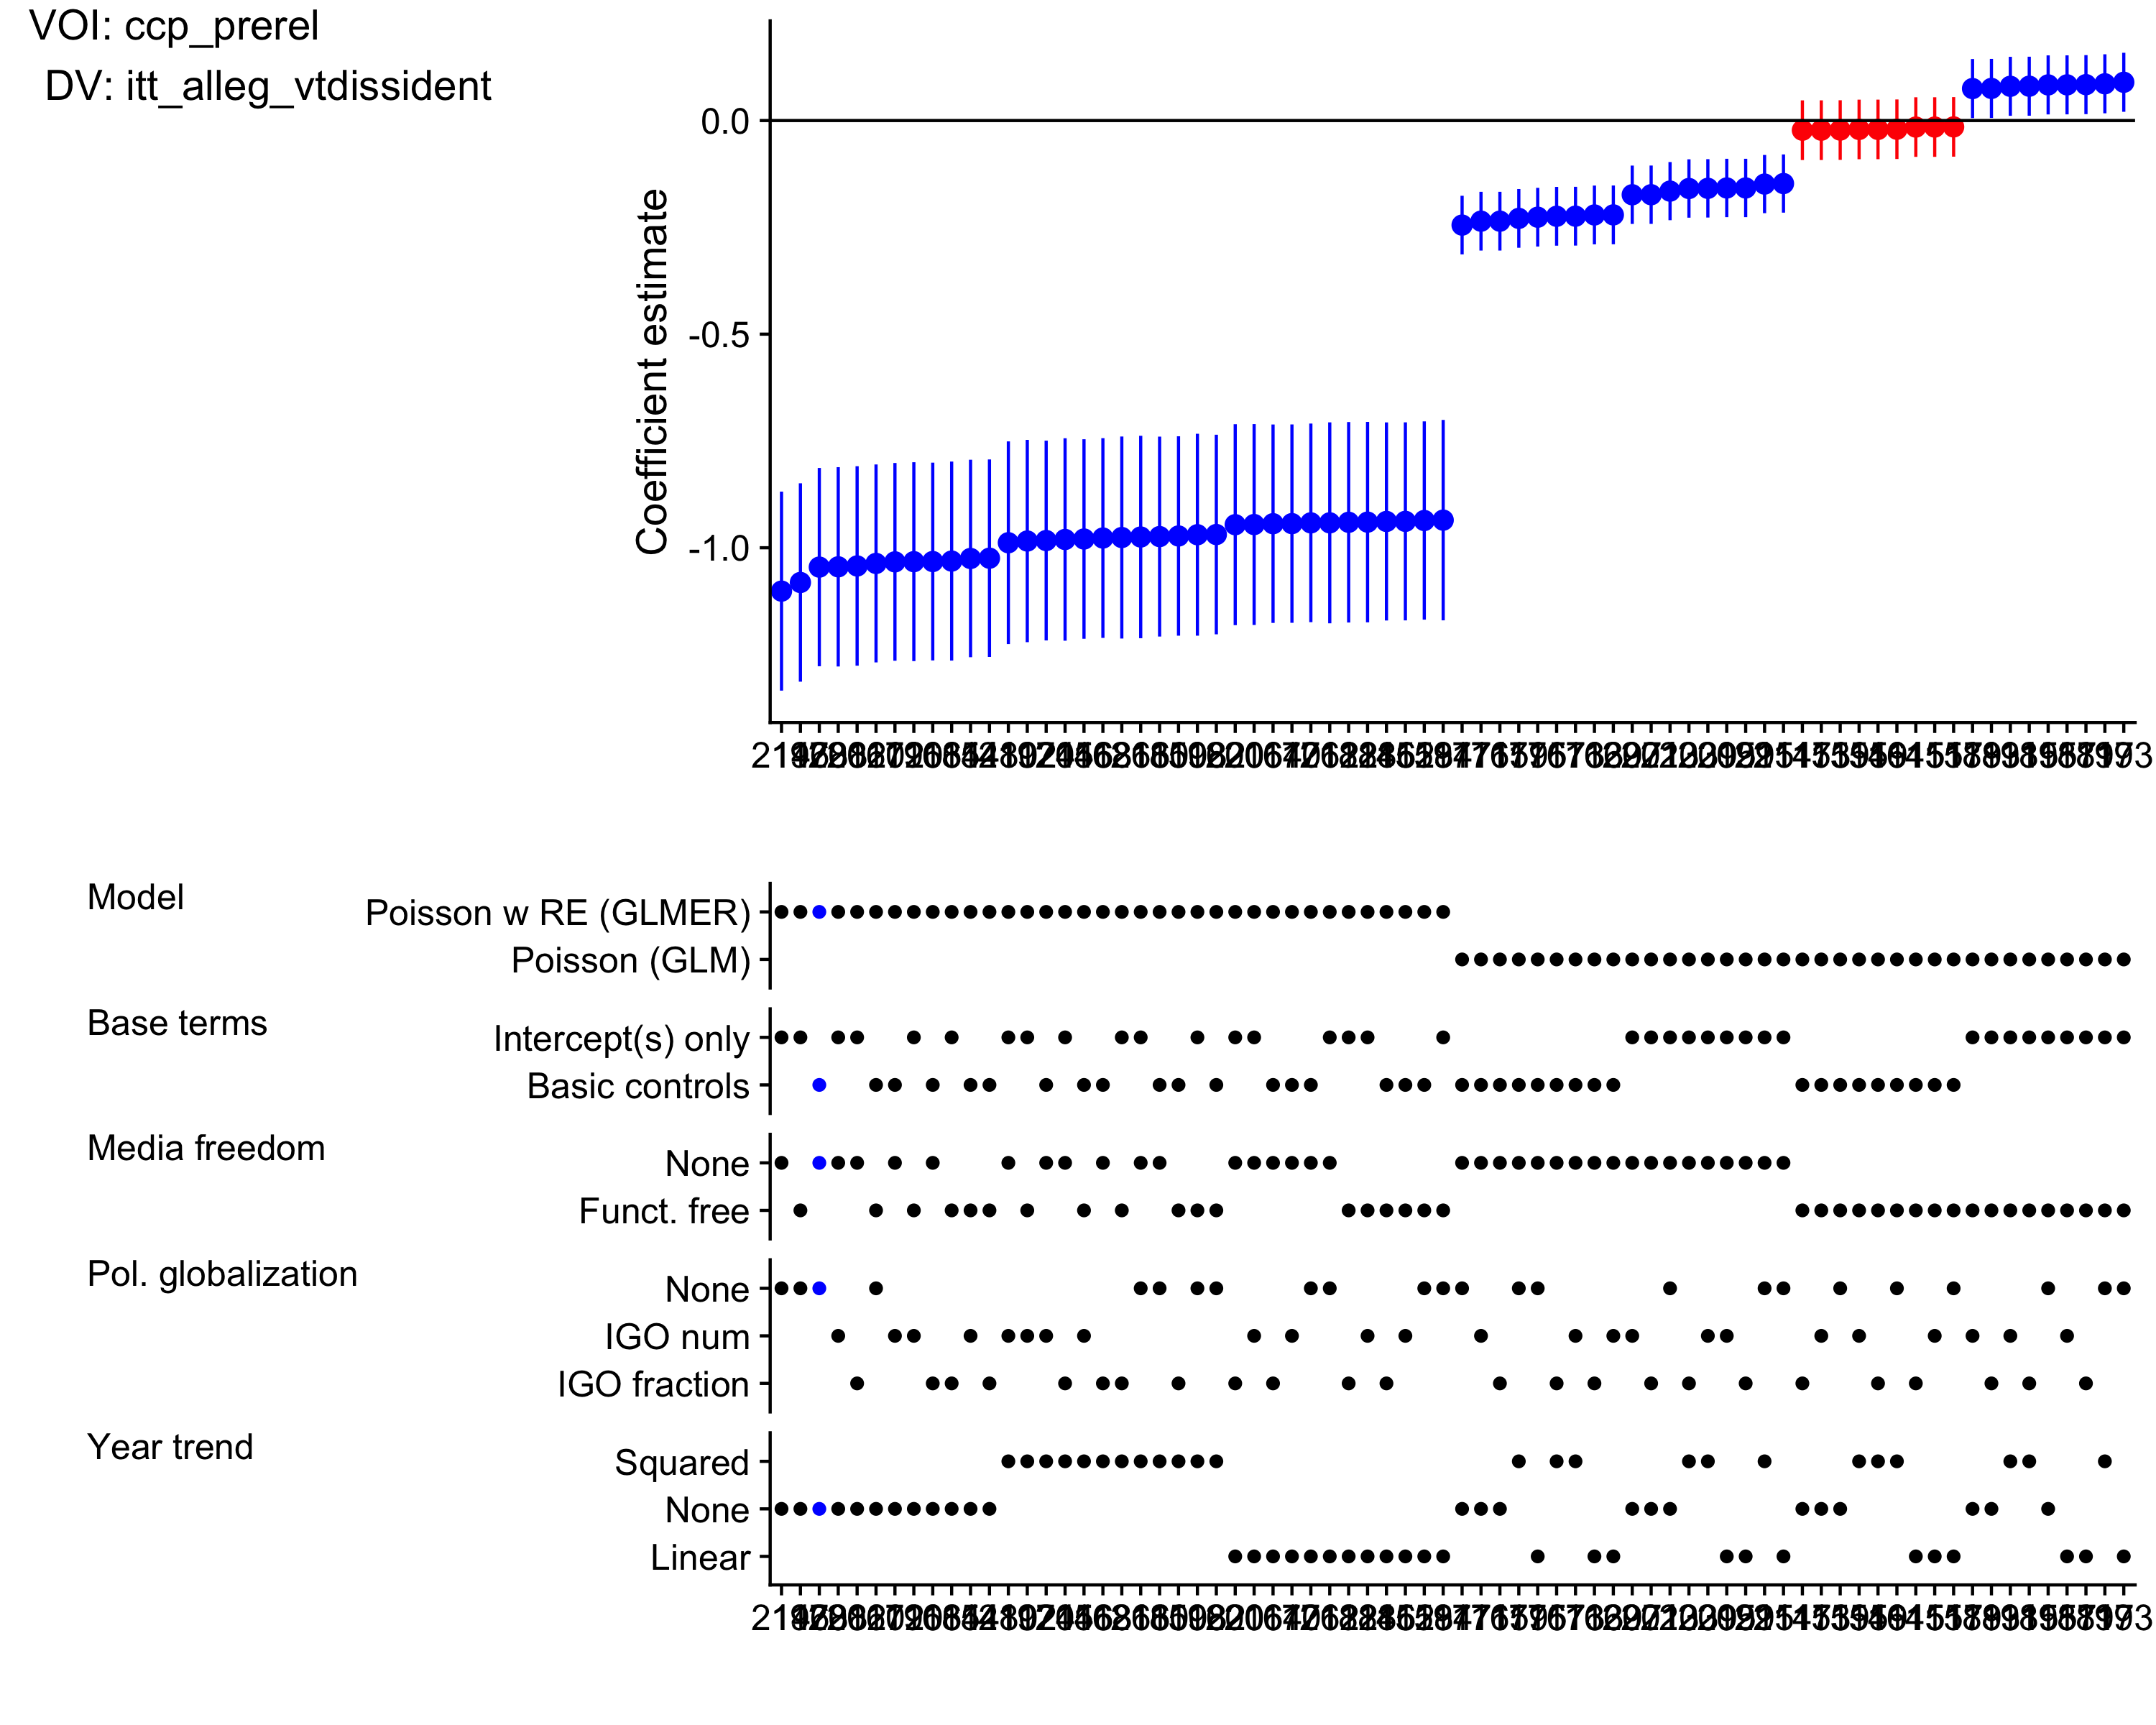
\includegraphics[height=4in]{../output/figures-robustness/specplot-ccp_prerel-itt_alleg_vtdissident.png}

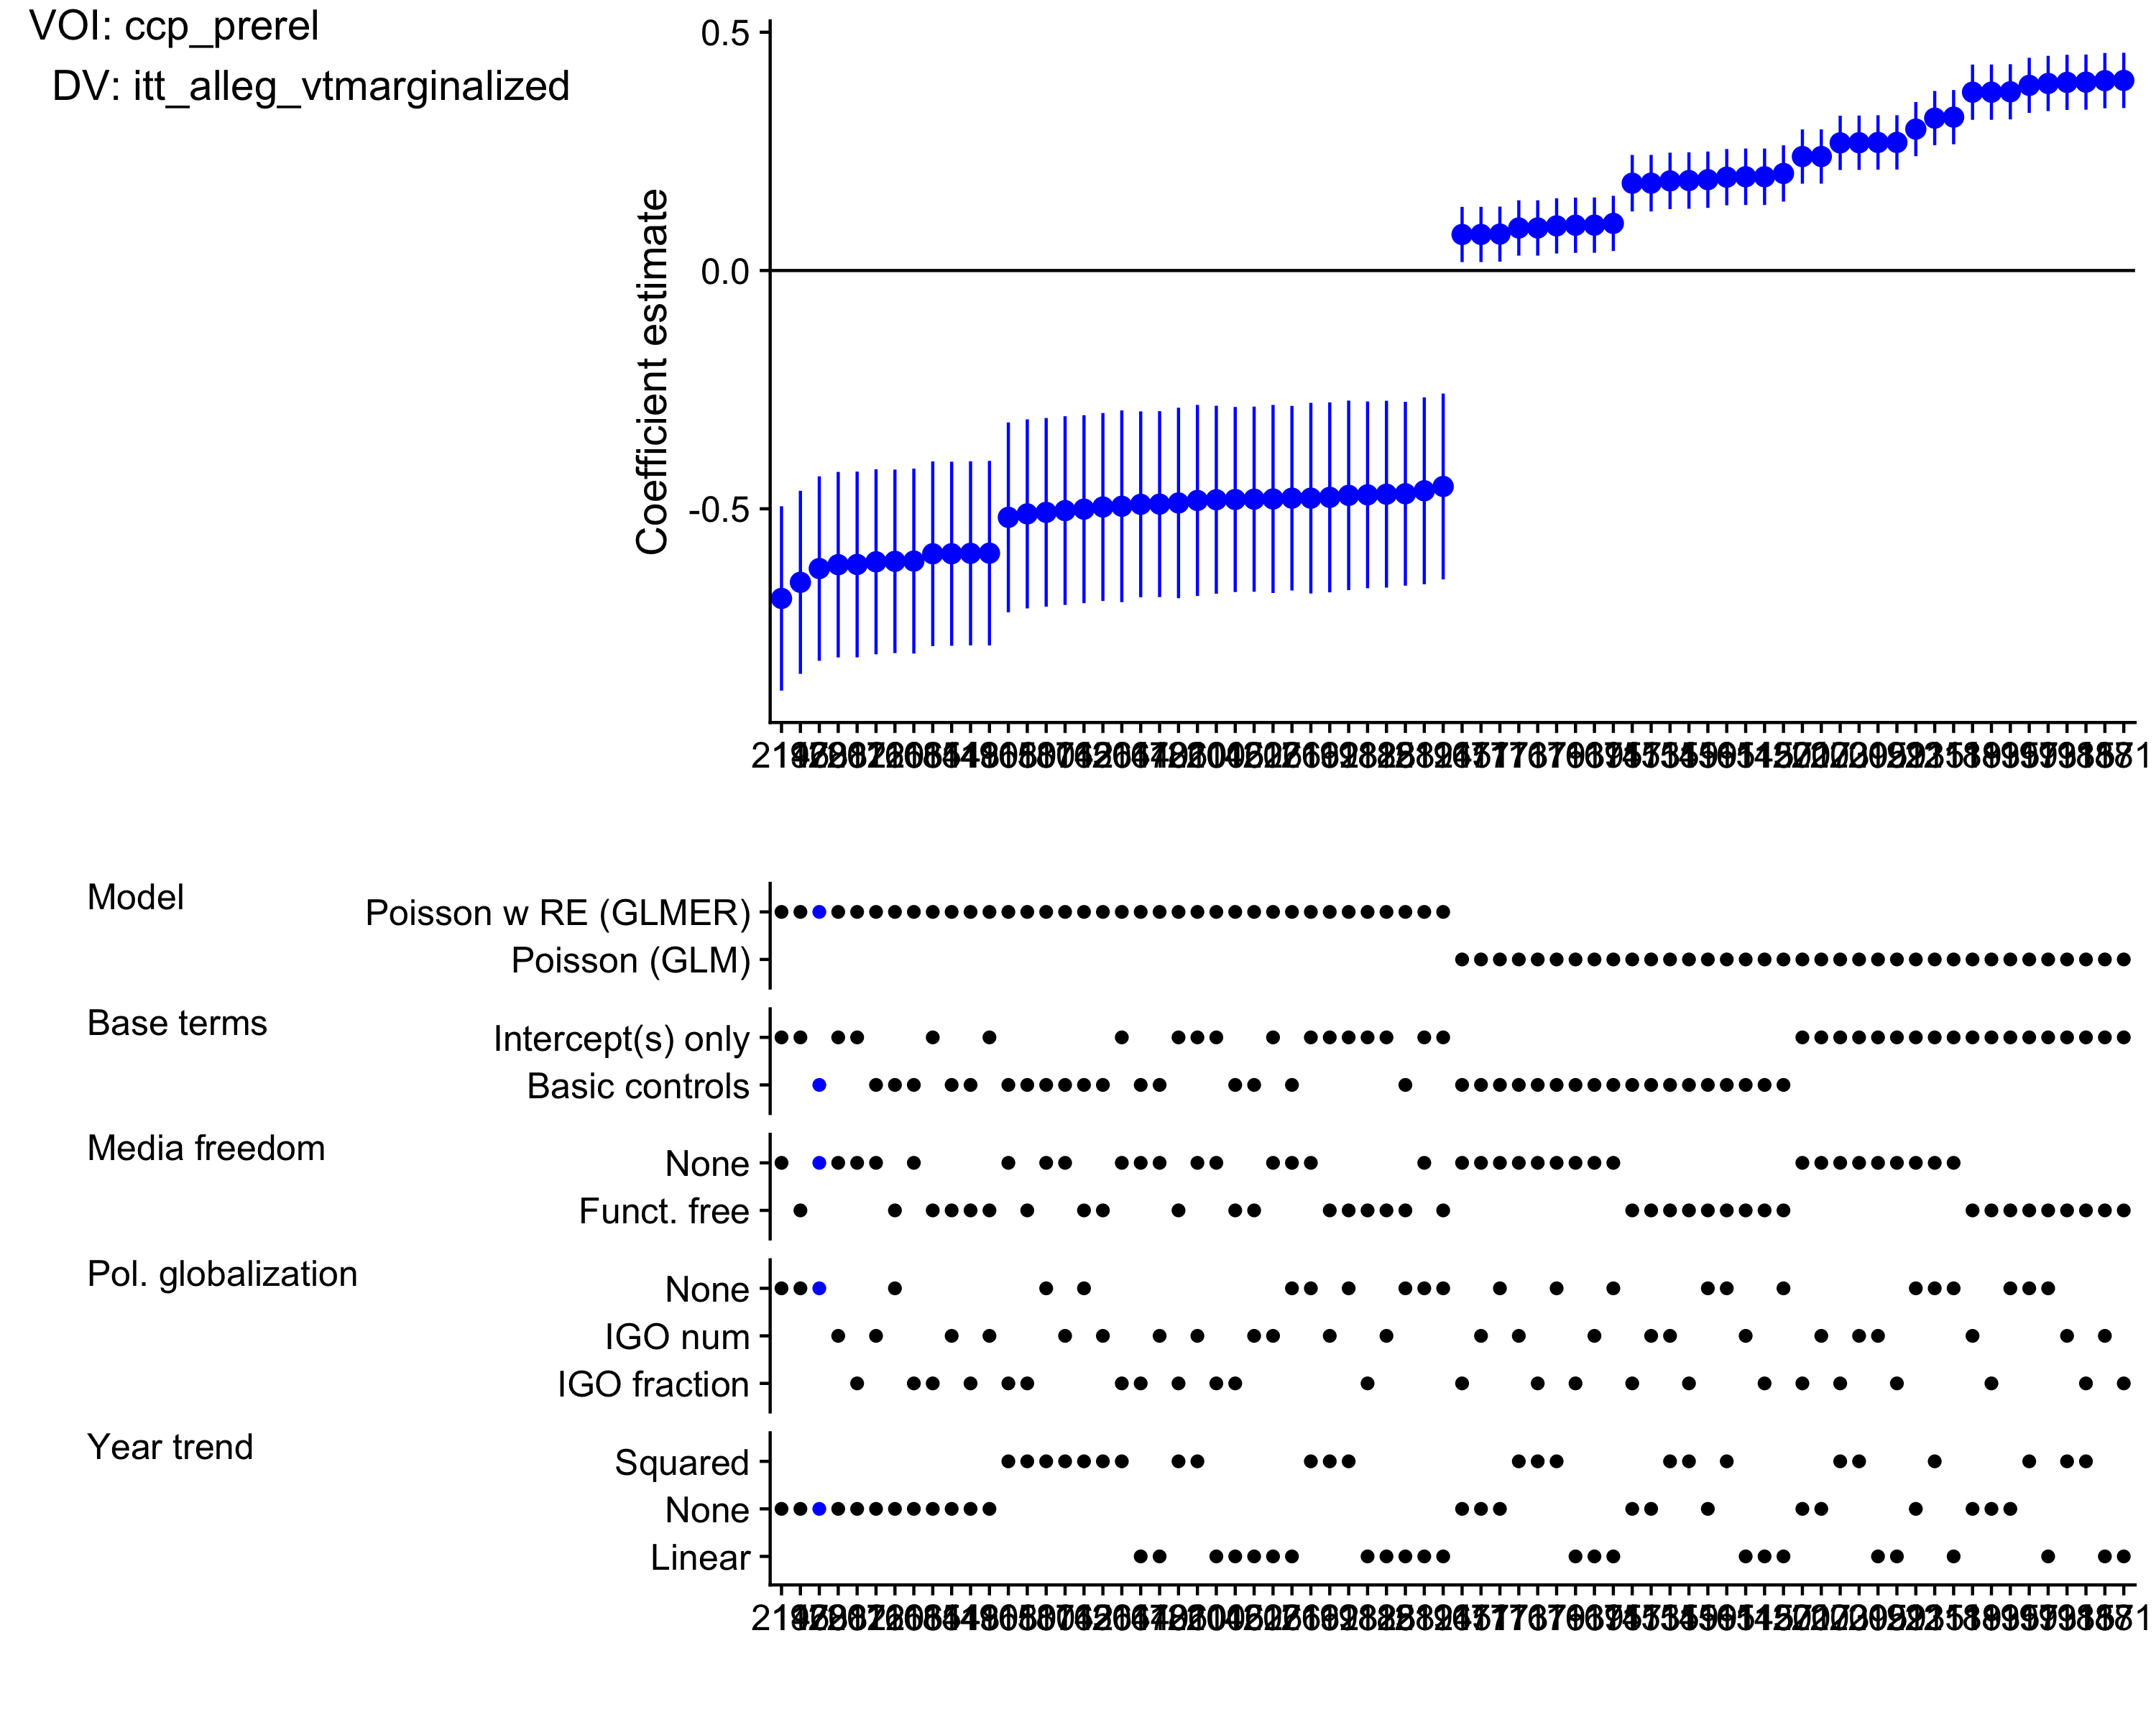
\includegraphics[height=4in]{../output/figures-robustness/specplot-ccp_prerel-itt_alleg_vtmarginalized.png}

\hypertarget{voi-ccp_speedtri}{%
\subsection{VOI: ccp\_speedtri}\label{voi-ccp_speedtri}}

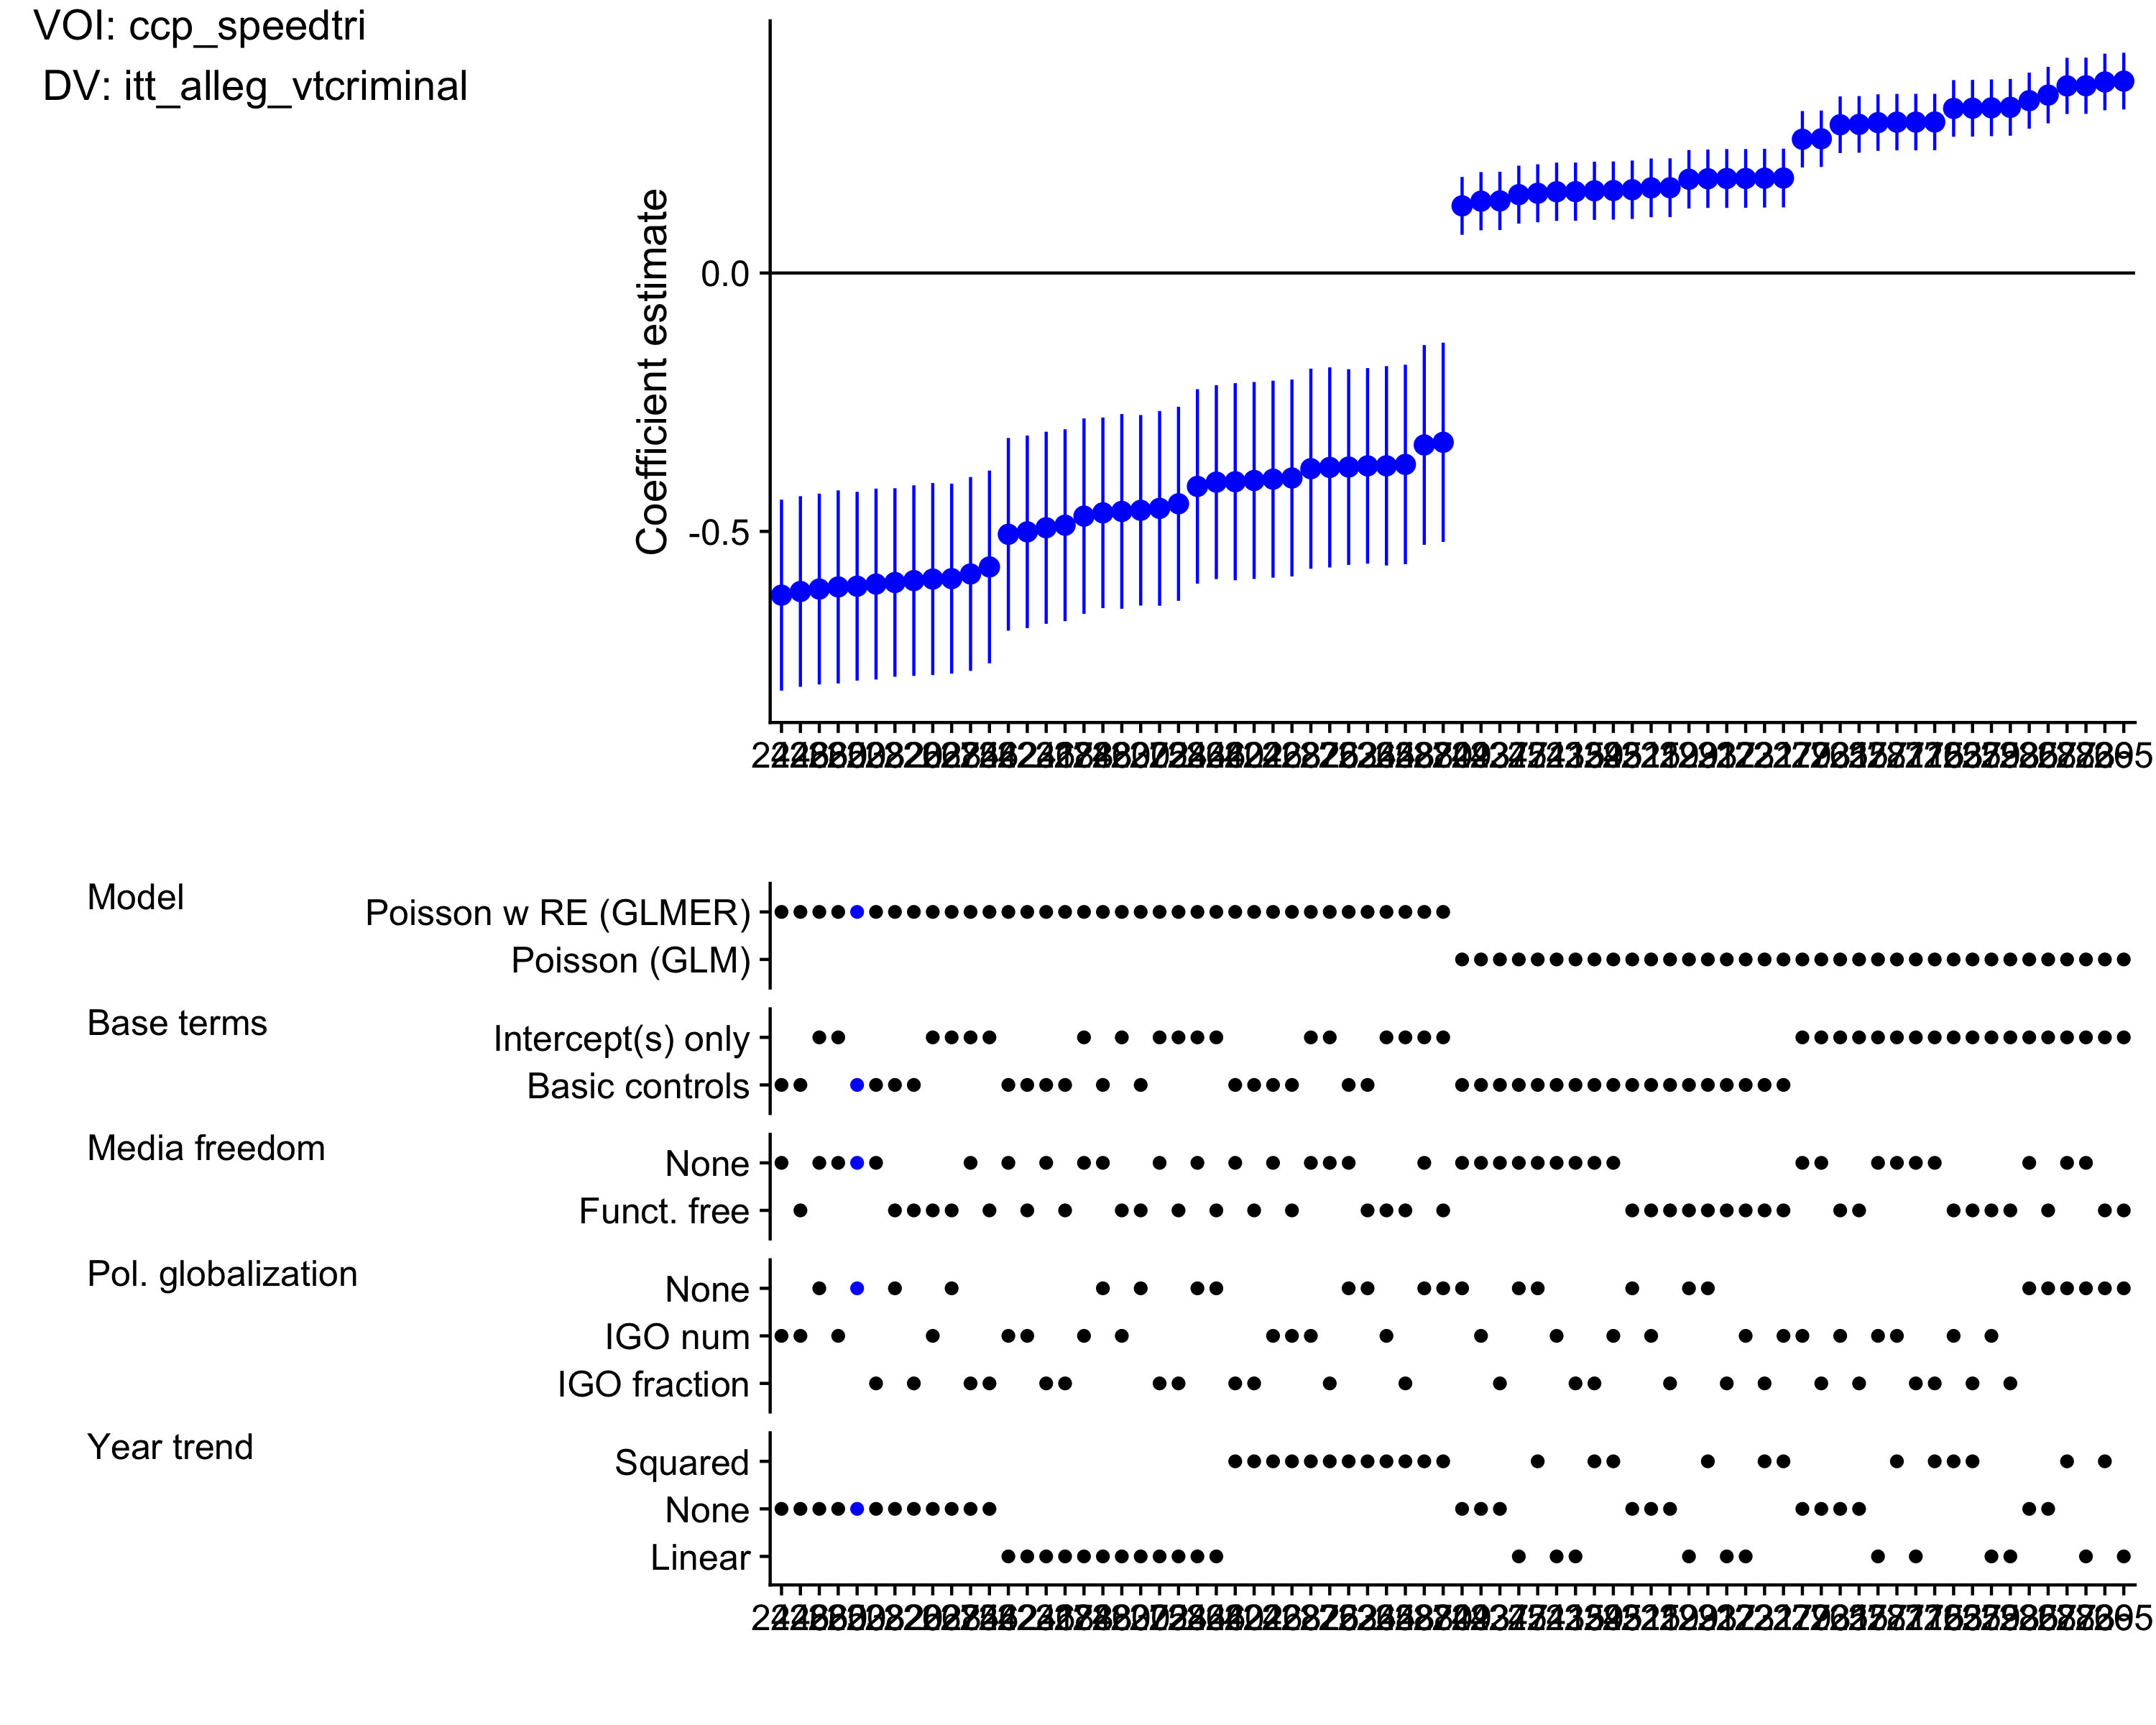
\includegraphics[height=4in]{../output/figures-robustness/specplot-ccp_speedtri-itt_alleg_vtcriminal.png}

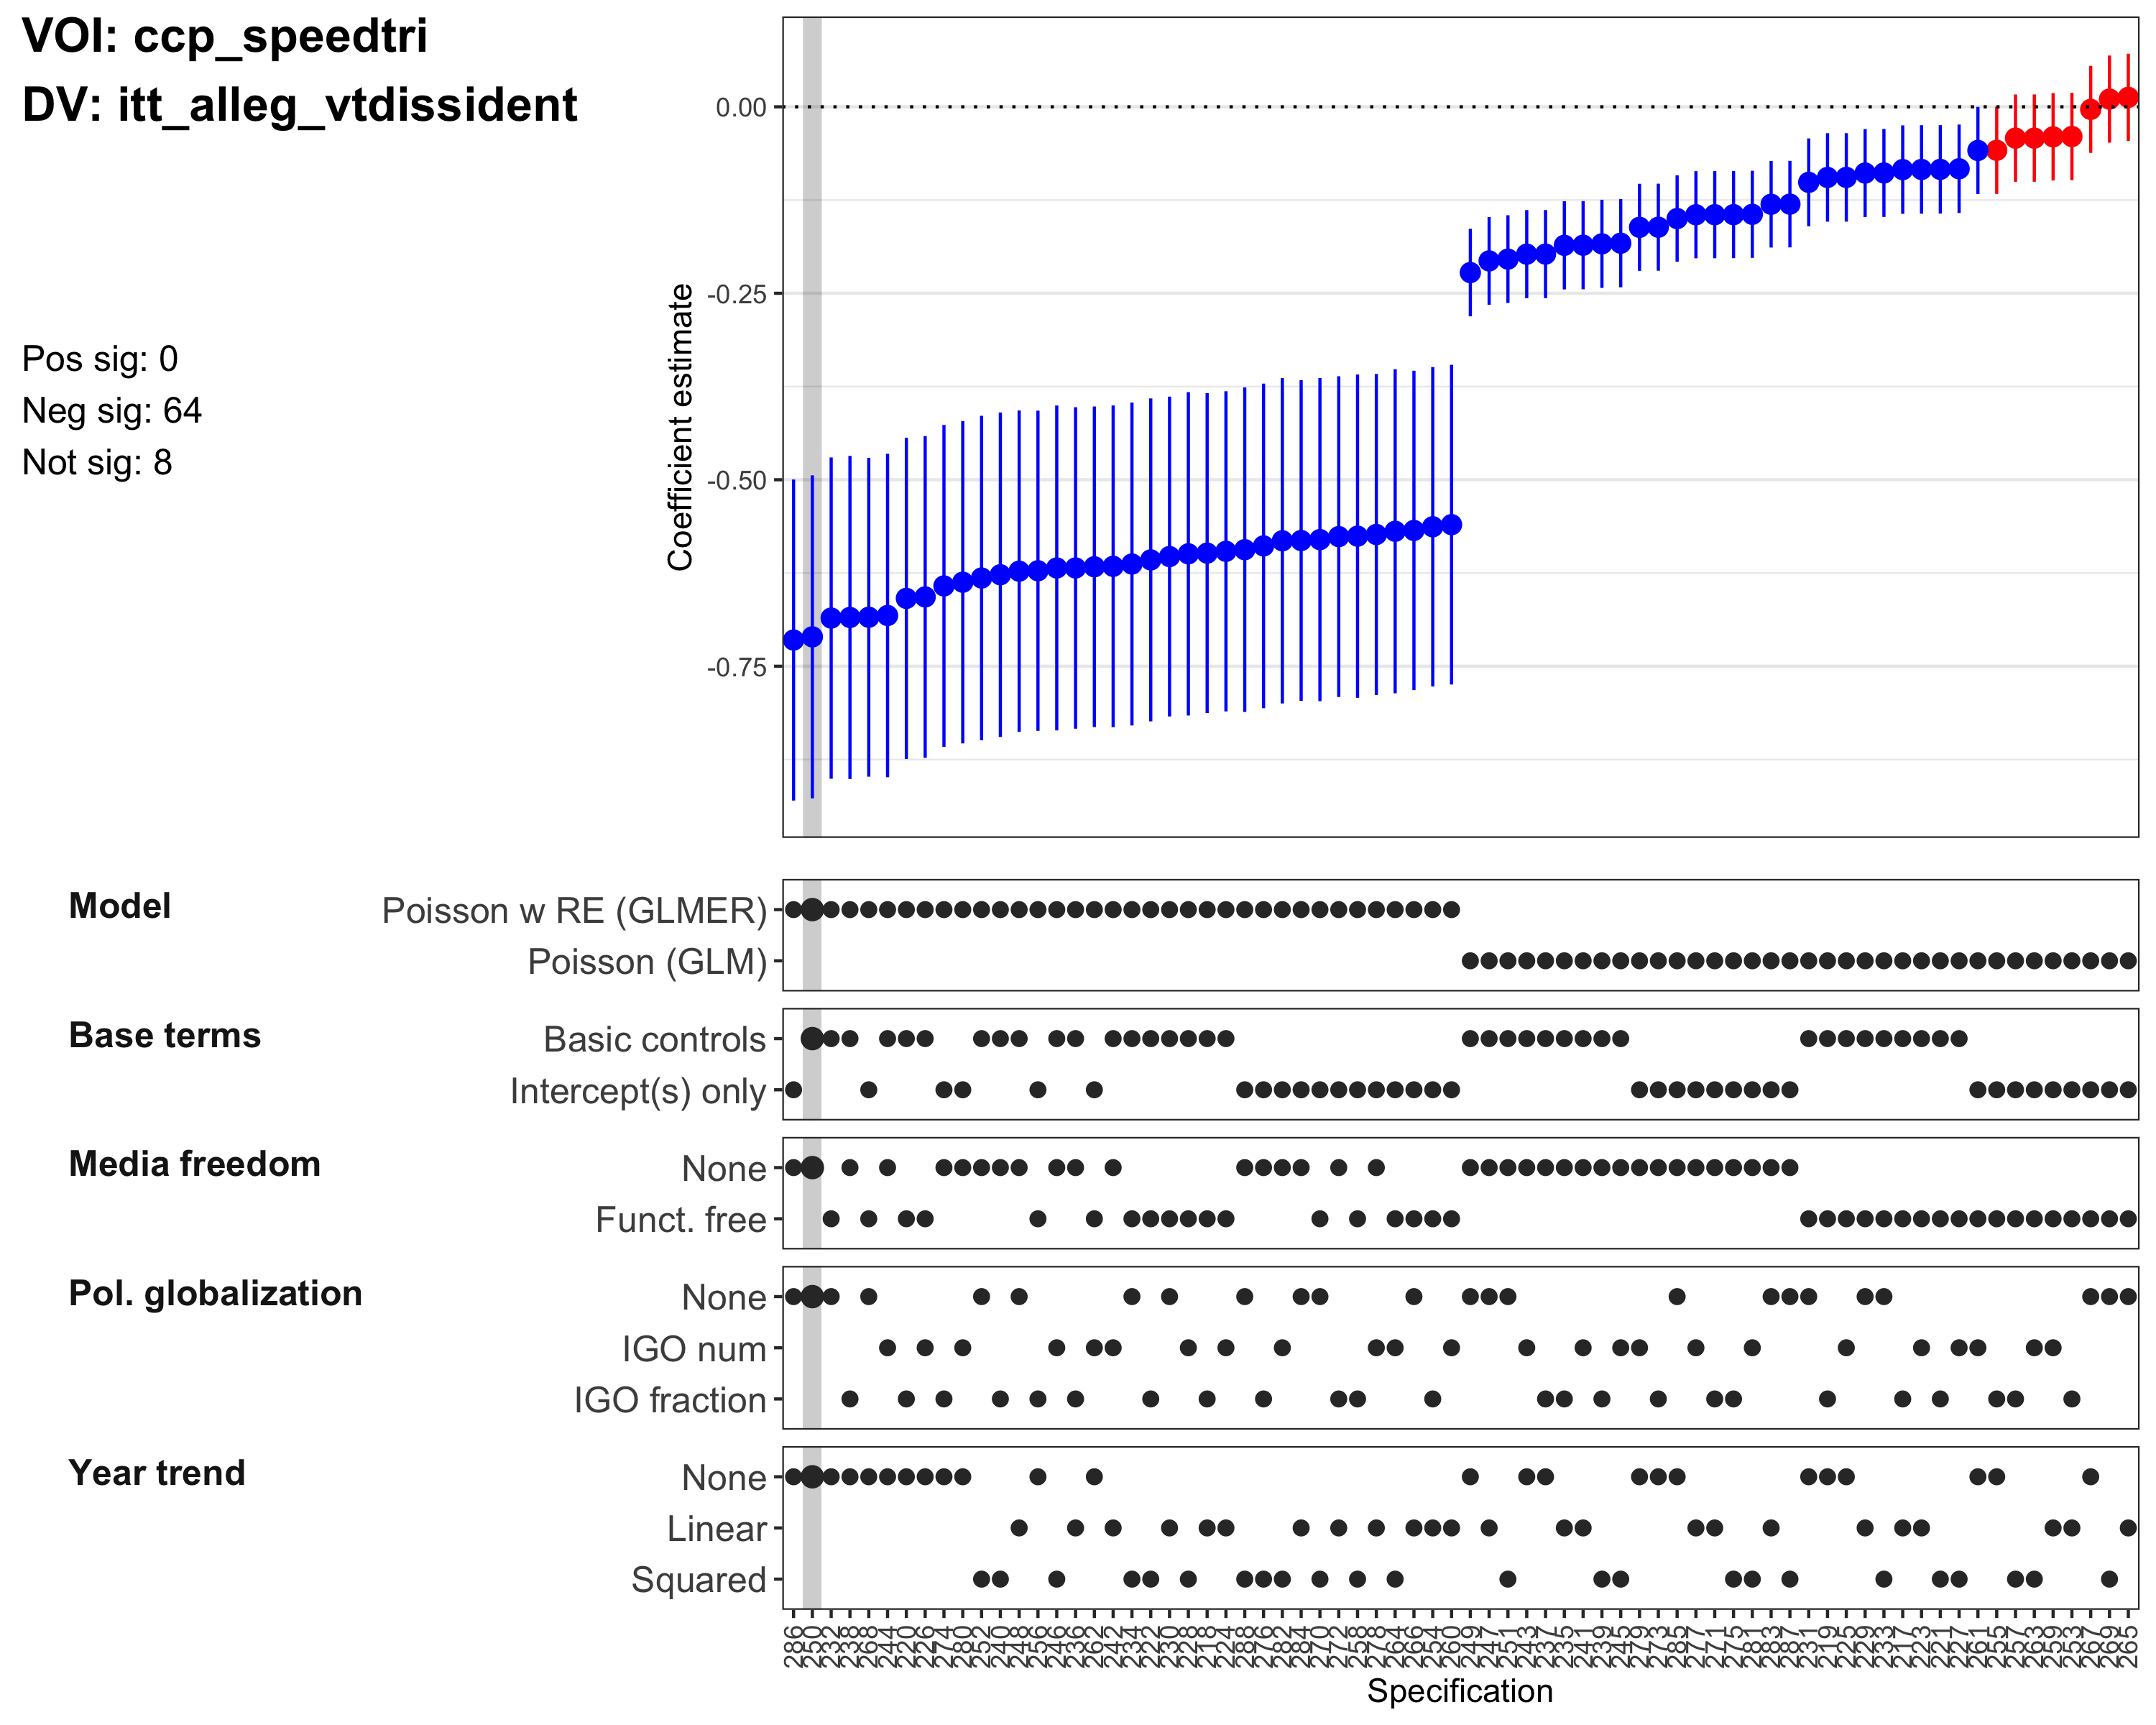
\includegraphics[height=4in]{../output/figures-robustness/specplot-ccp_speedtri-itt_alleg_vtdissident.png}

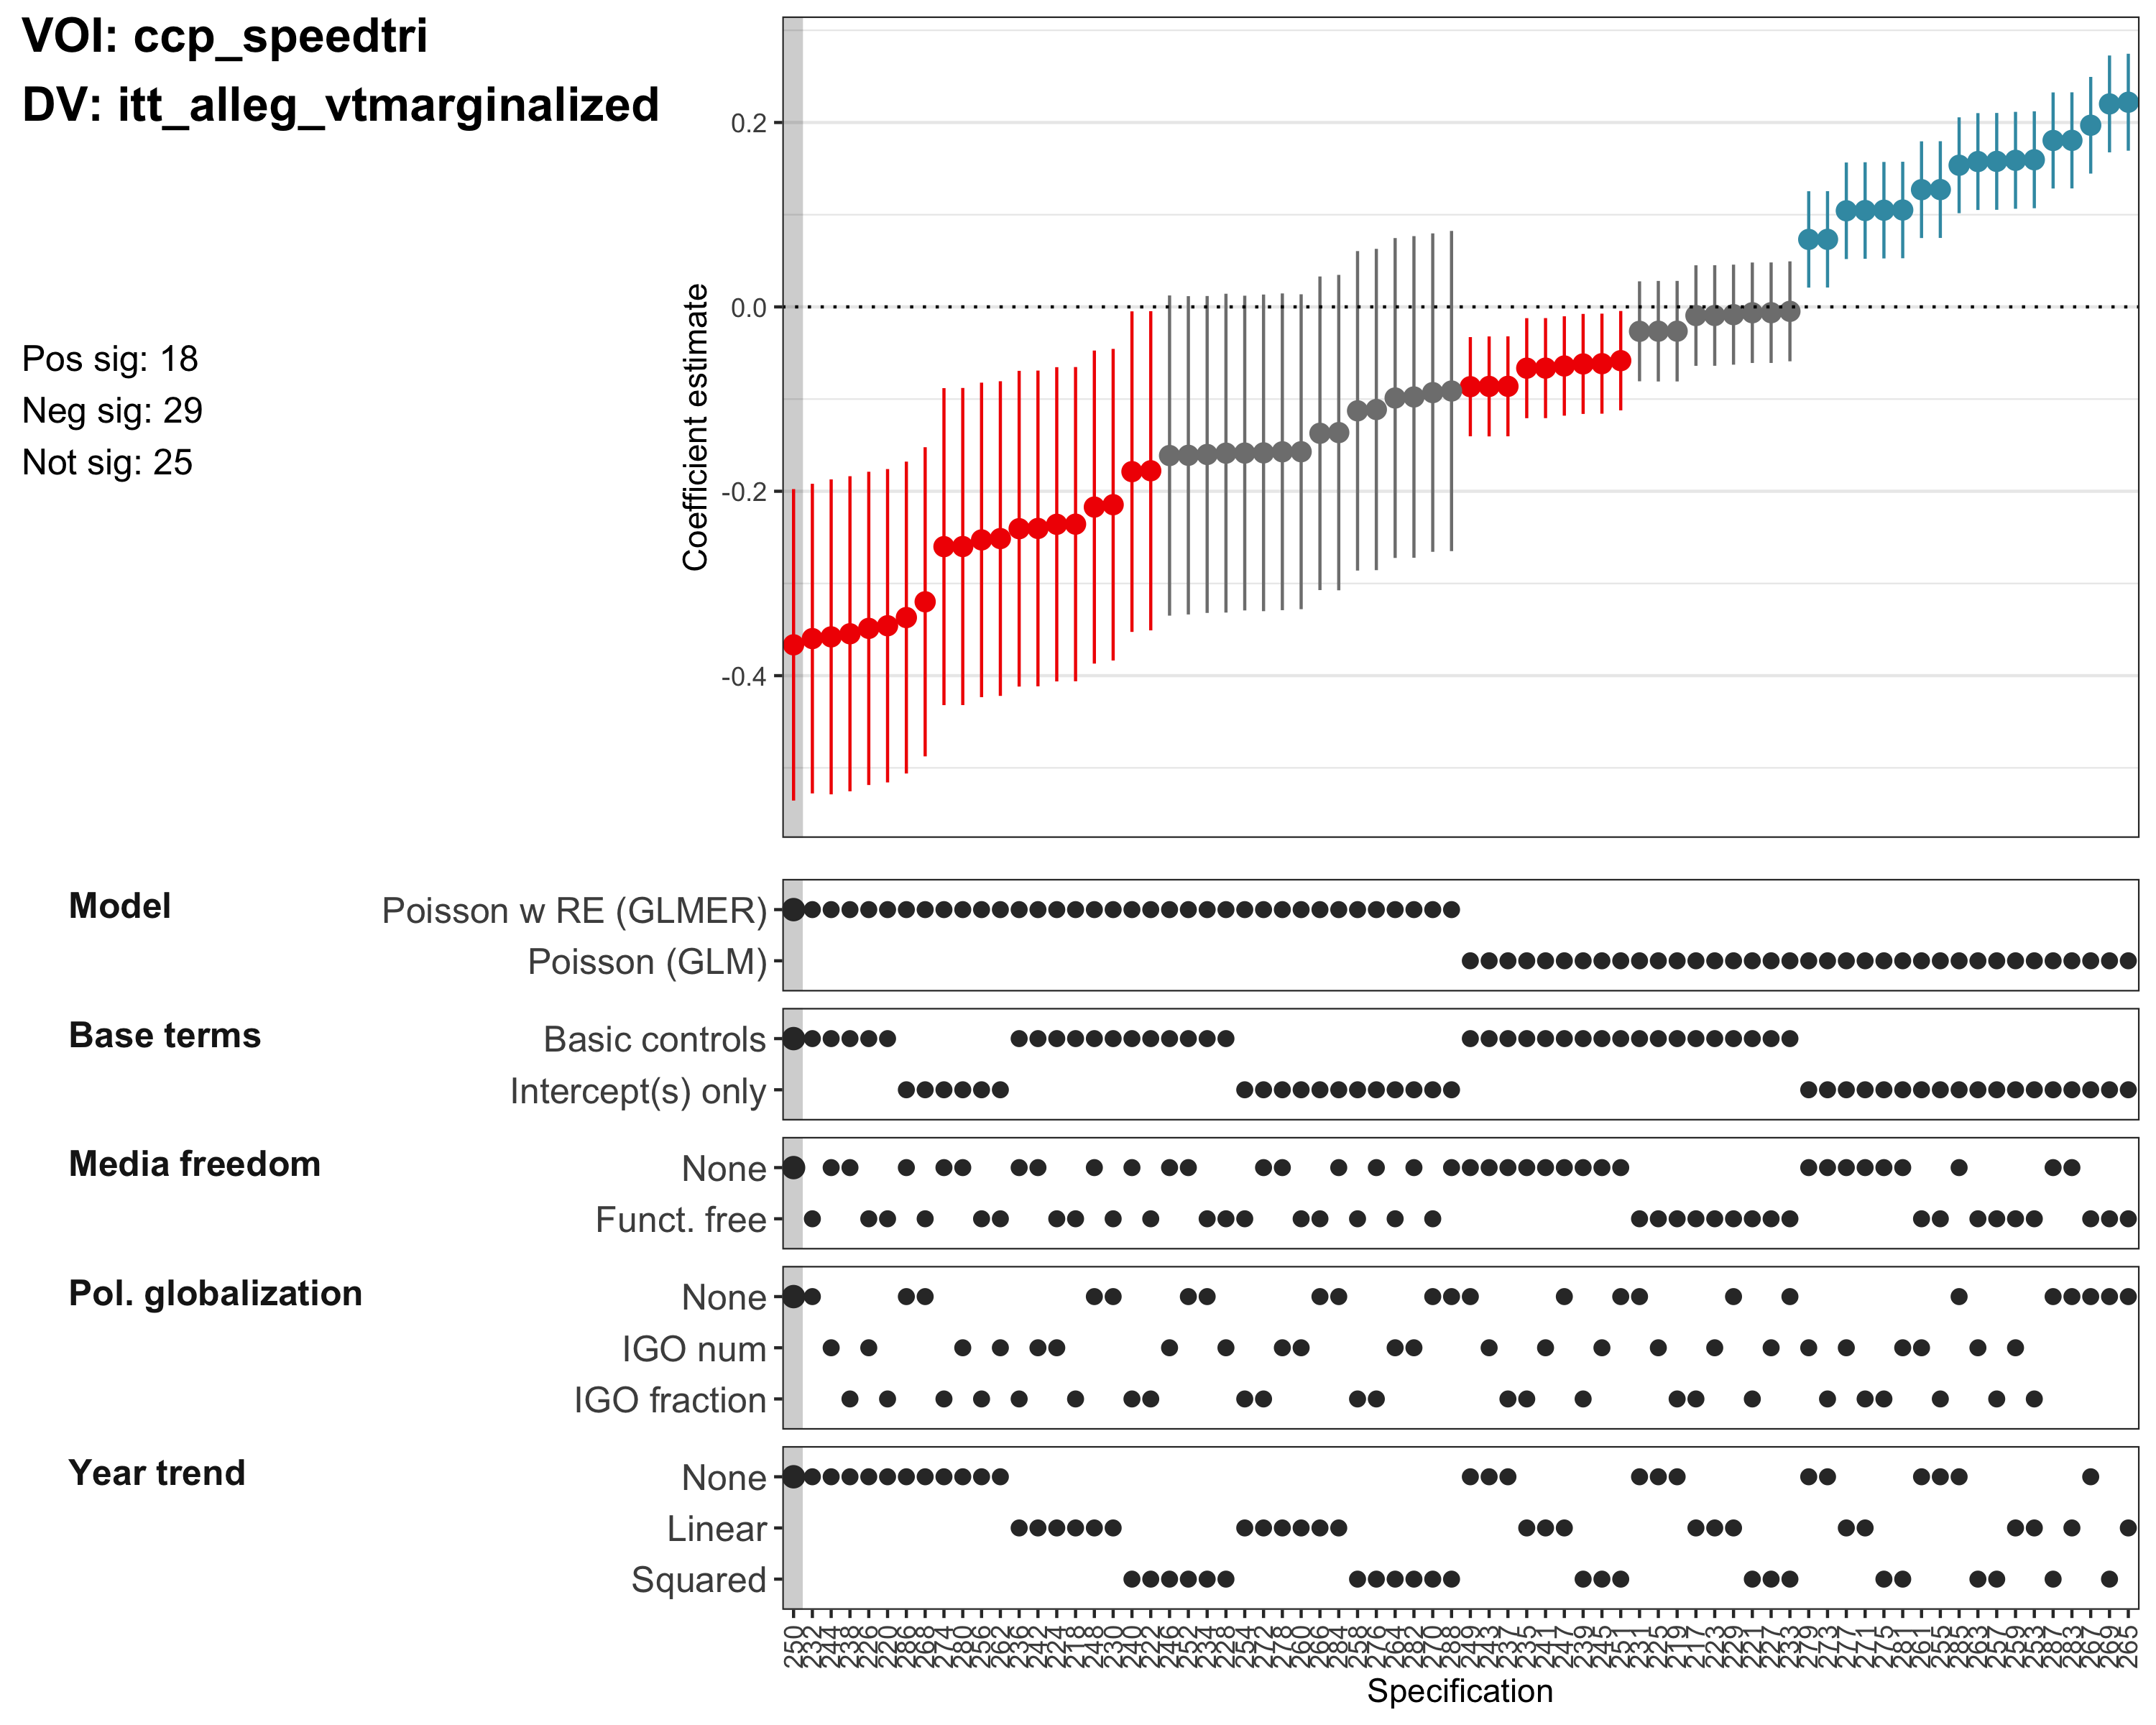
\includegraphics[height=4in]{../output/figures-robustness/specplot-ccp_speedtri-itt_alleg_vtmarginalized.png}

\hypertarget{voi-ccp_torture}{%
\subsection{VOI: ccp\_torture}\label{voi-ccp_torture}}

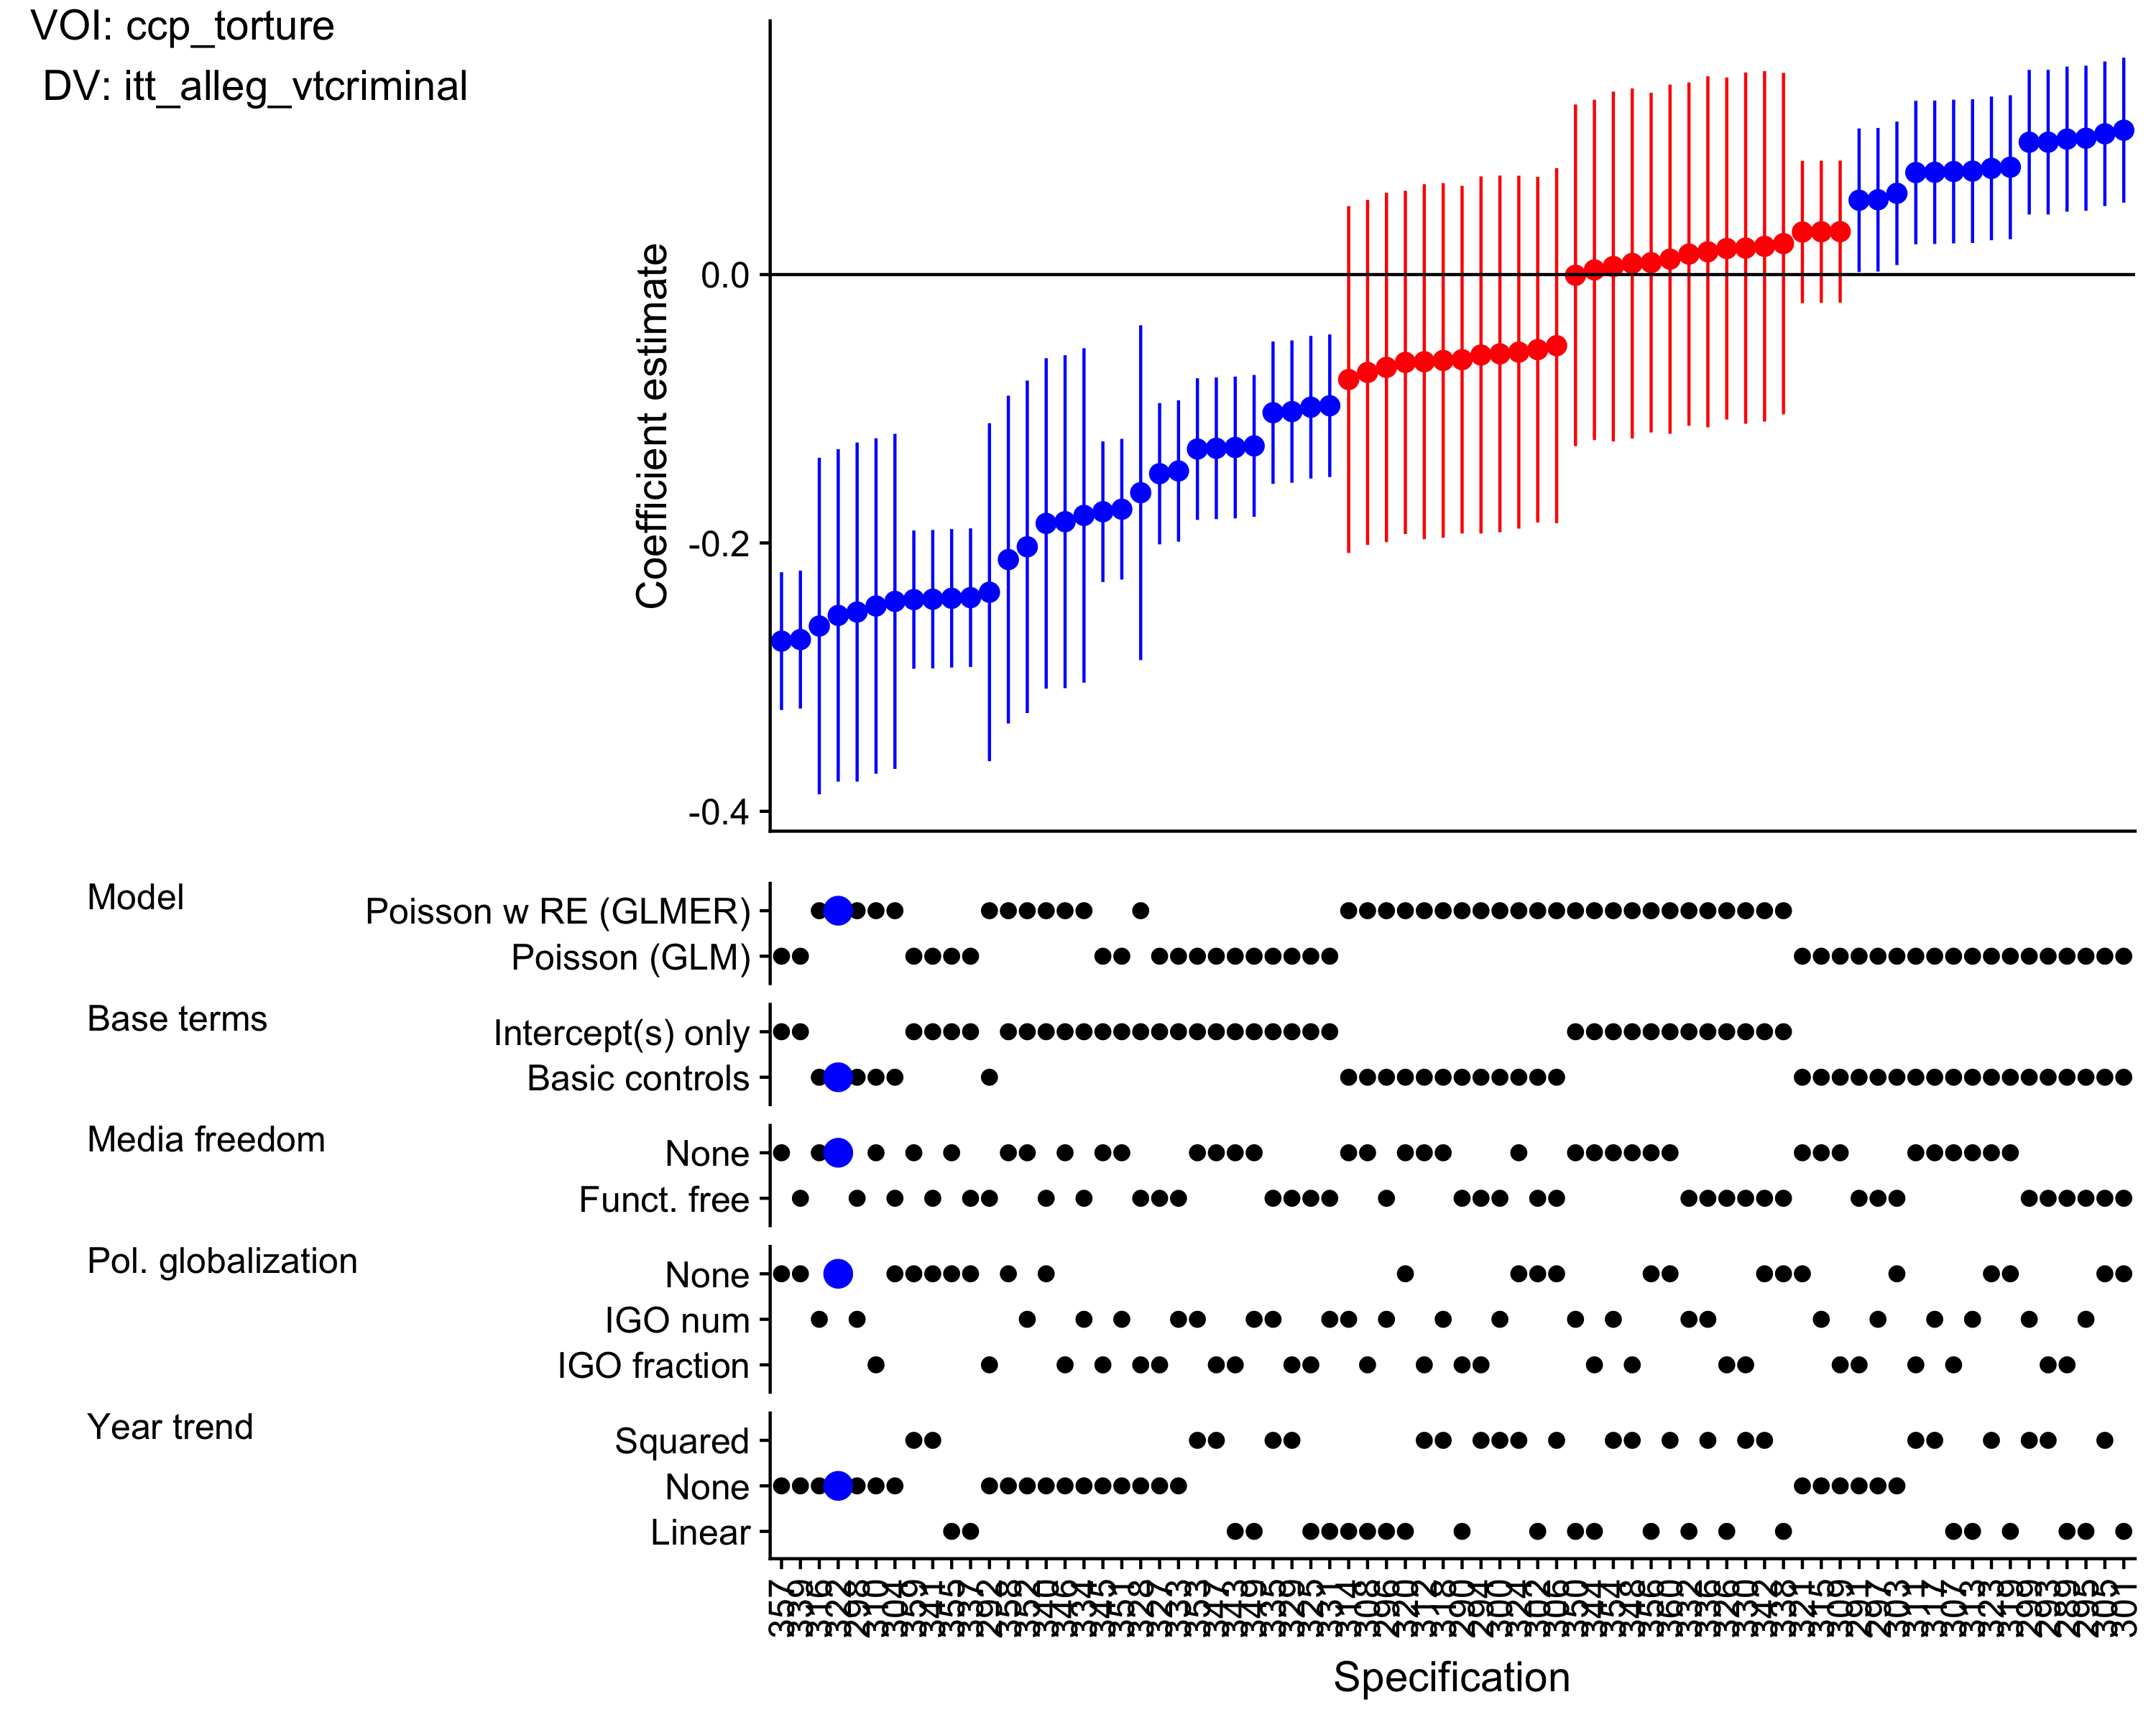
\includegraphics[height=4in]{../output/figures-robustness/specplot-ccp_torture-itt_alleg_vtcriminal.png}

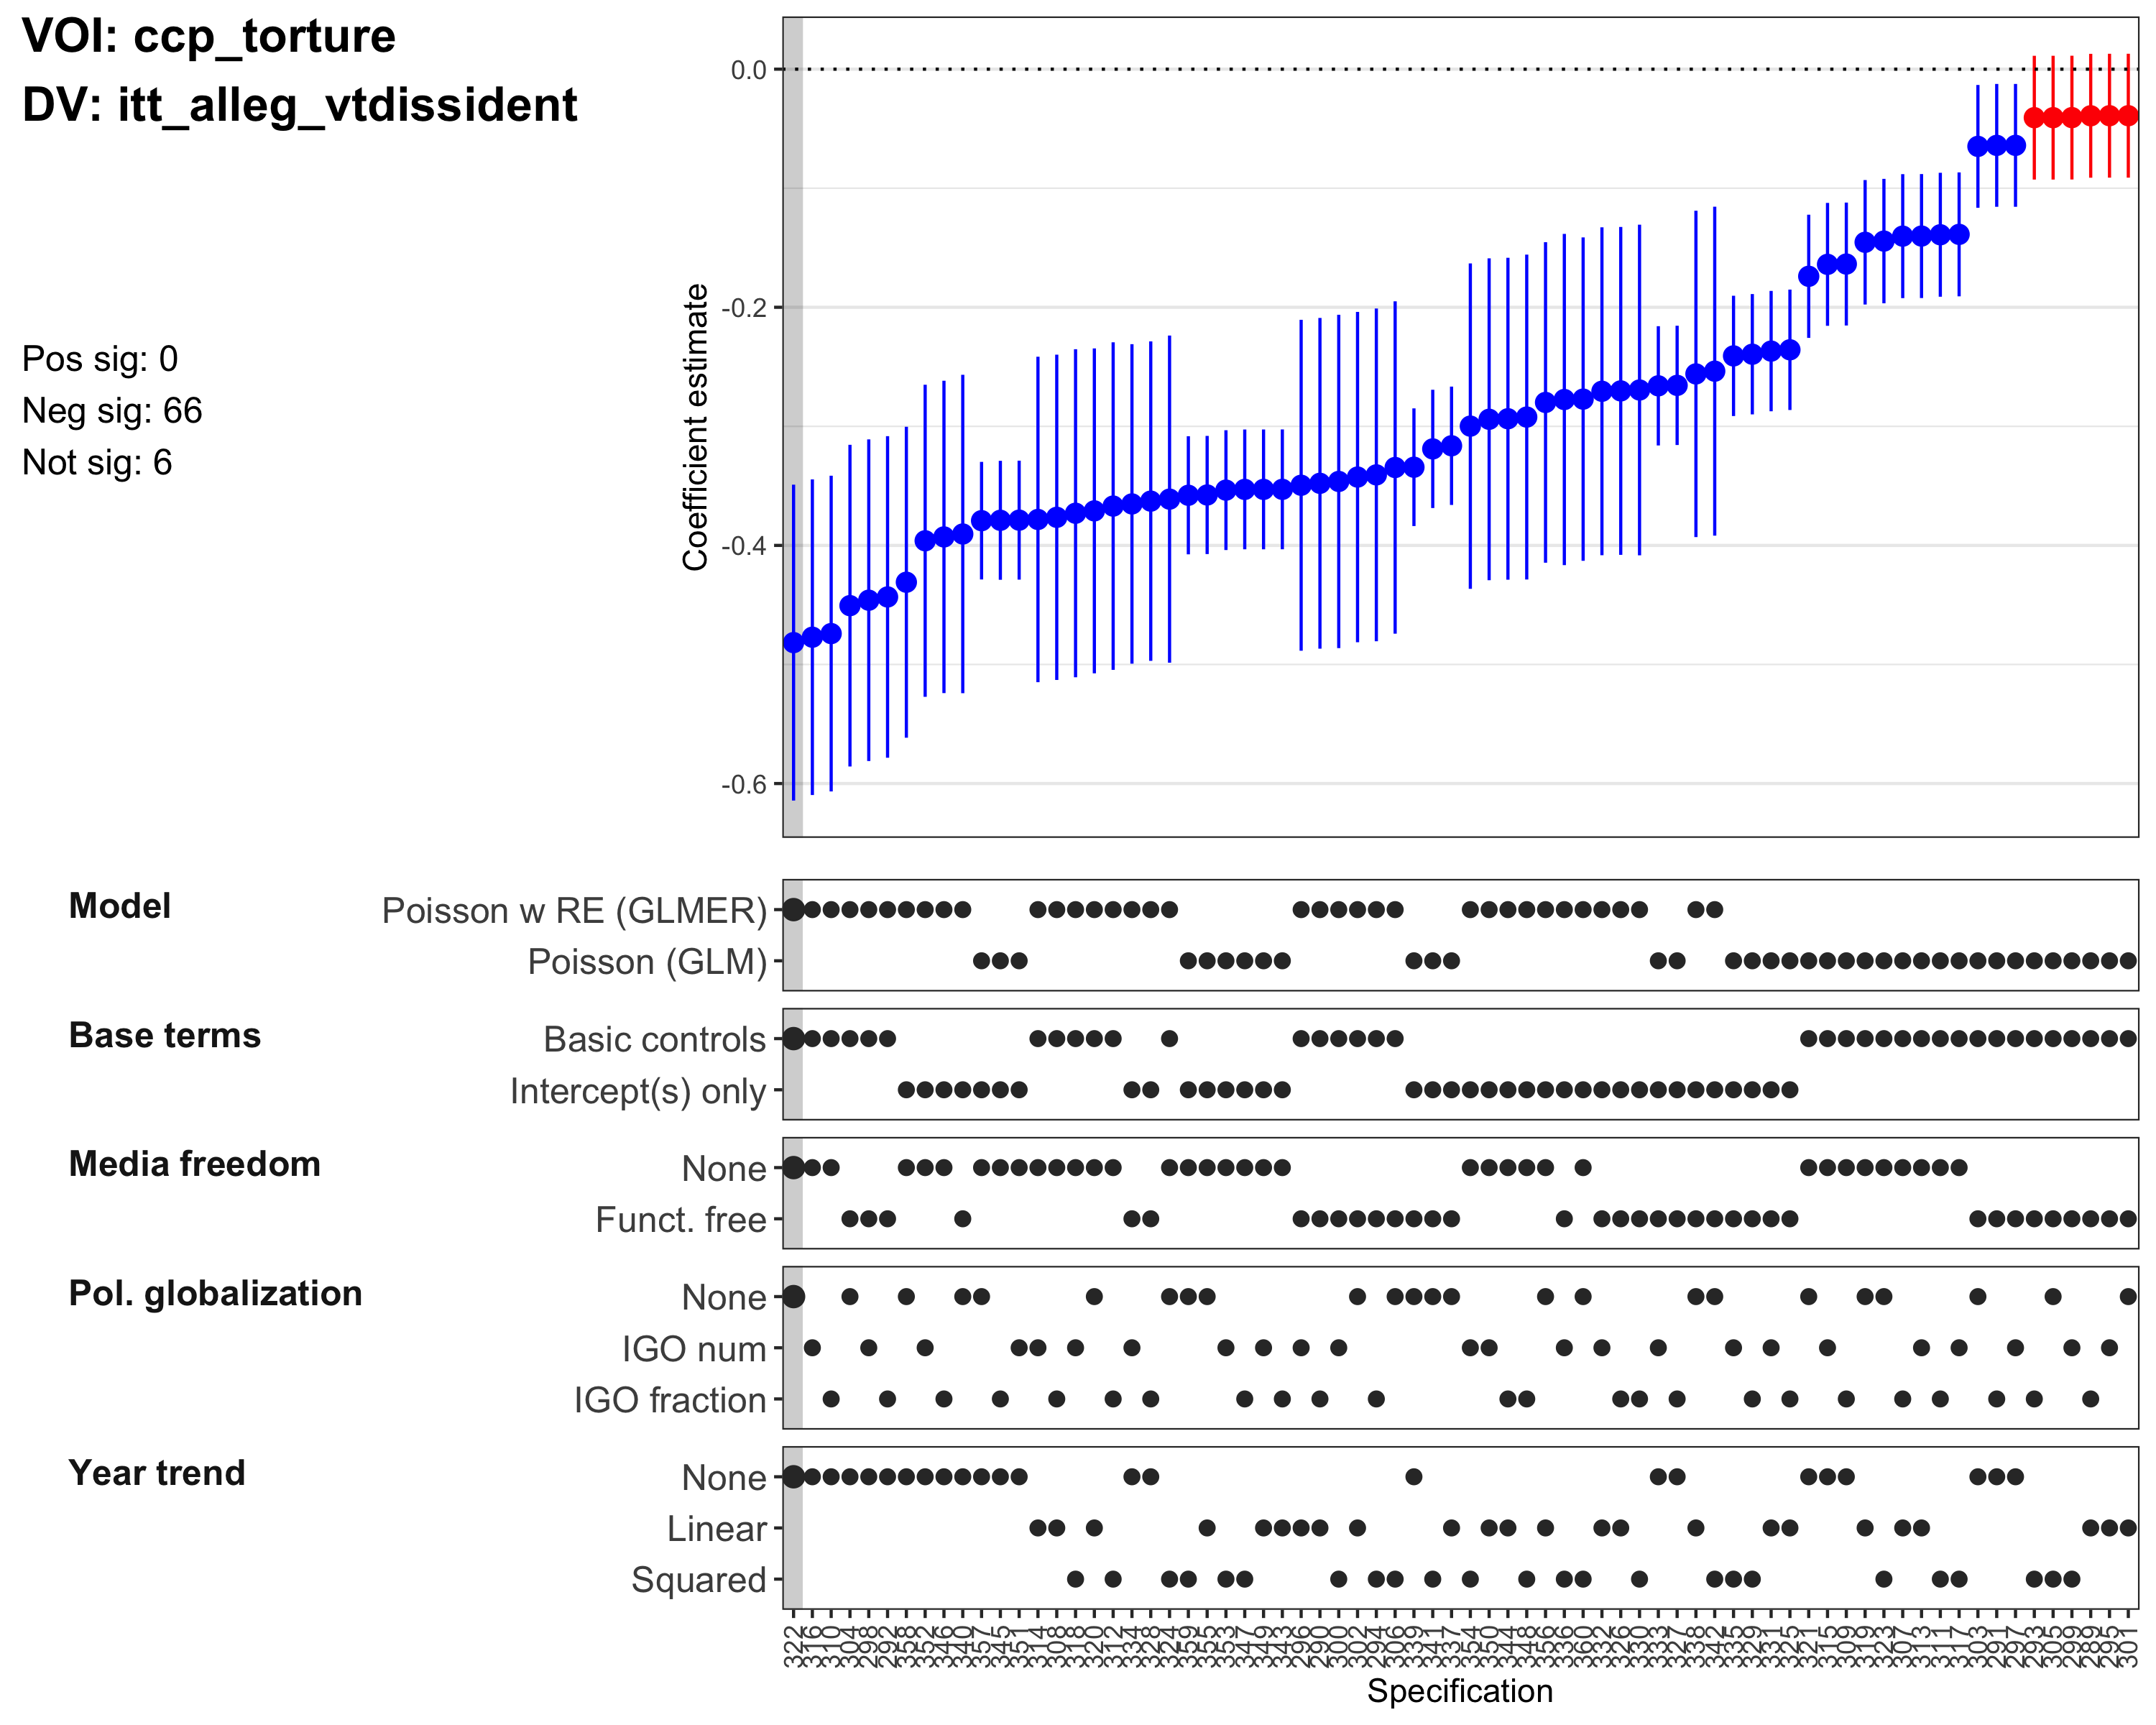
\includegraphics[height=4in]{../output/figures-robustness/specplot-ccp_torture-itt_alleg_vtdissident.png}

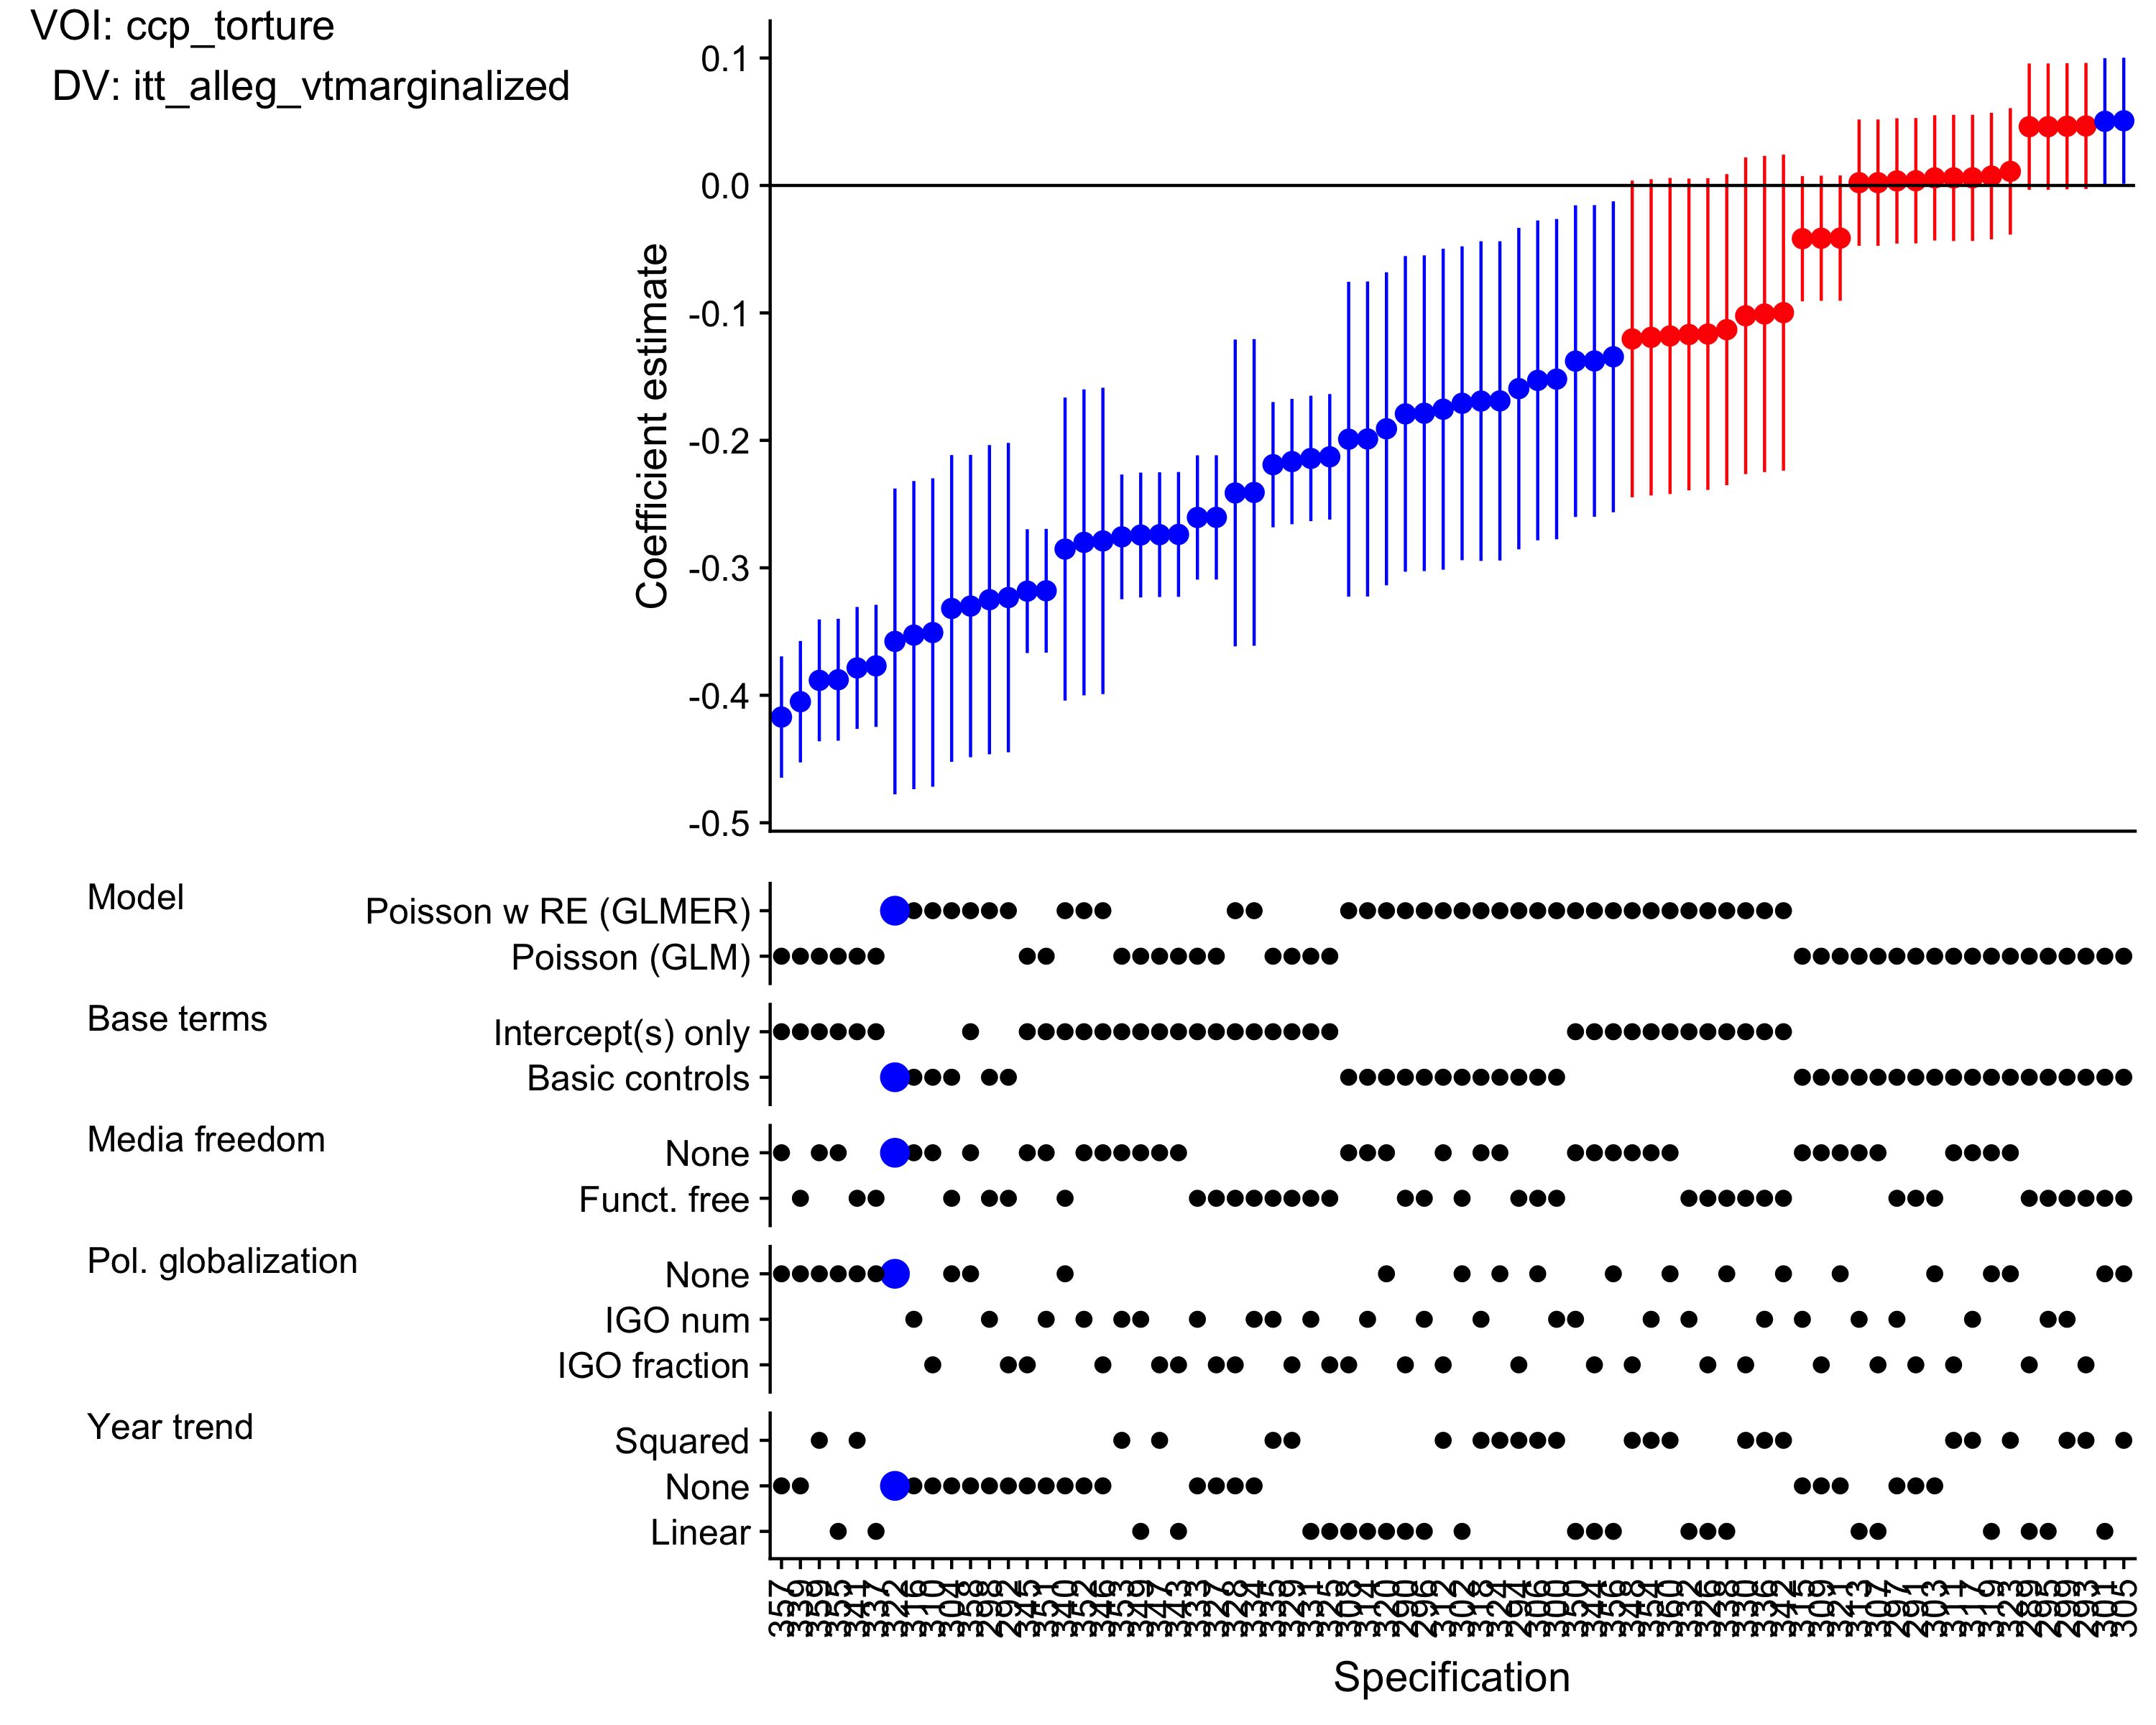
\includegraphics[height=4in]{../output/figures-robustness/specplot-ccp_torture-itt_alleg_vtmarginalized.png}

\hypertarget{voi-dd_democracy}{%
\subsection{VOI: dd\_democracy}\label{voi-dd_democracy}}

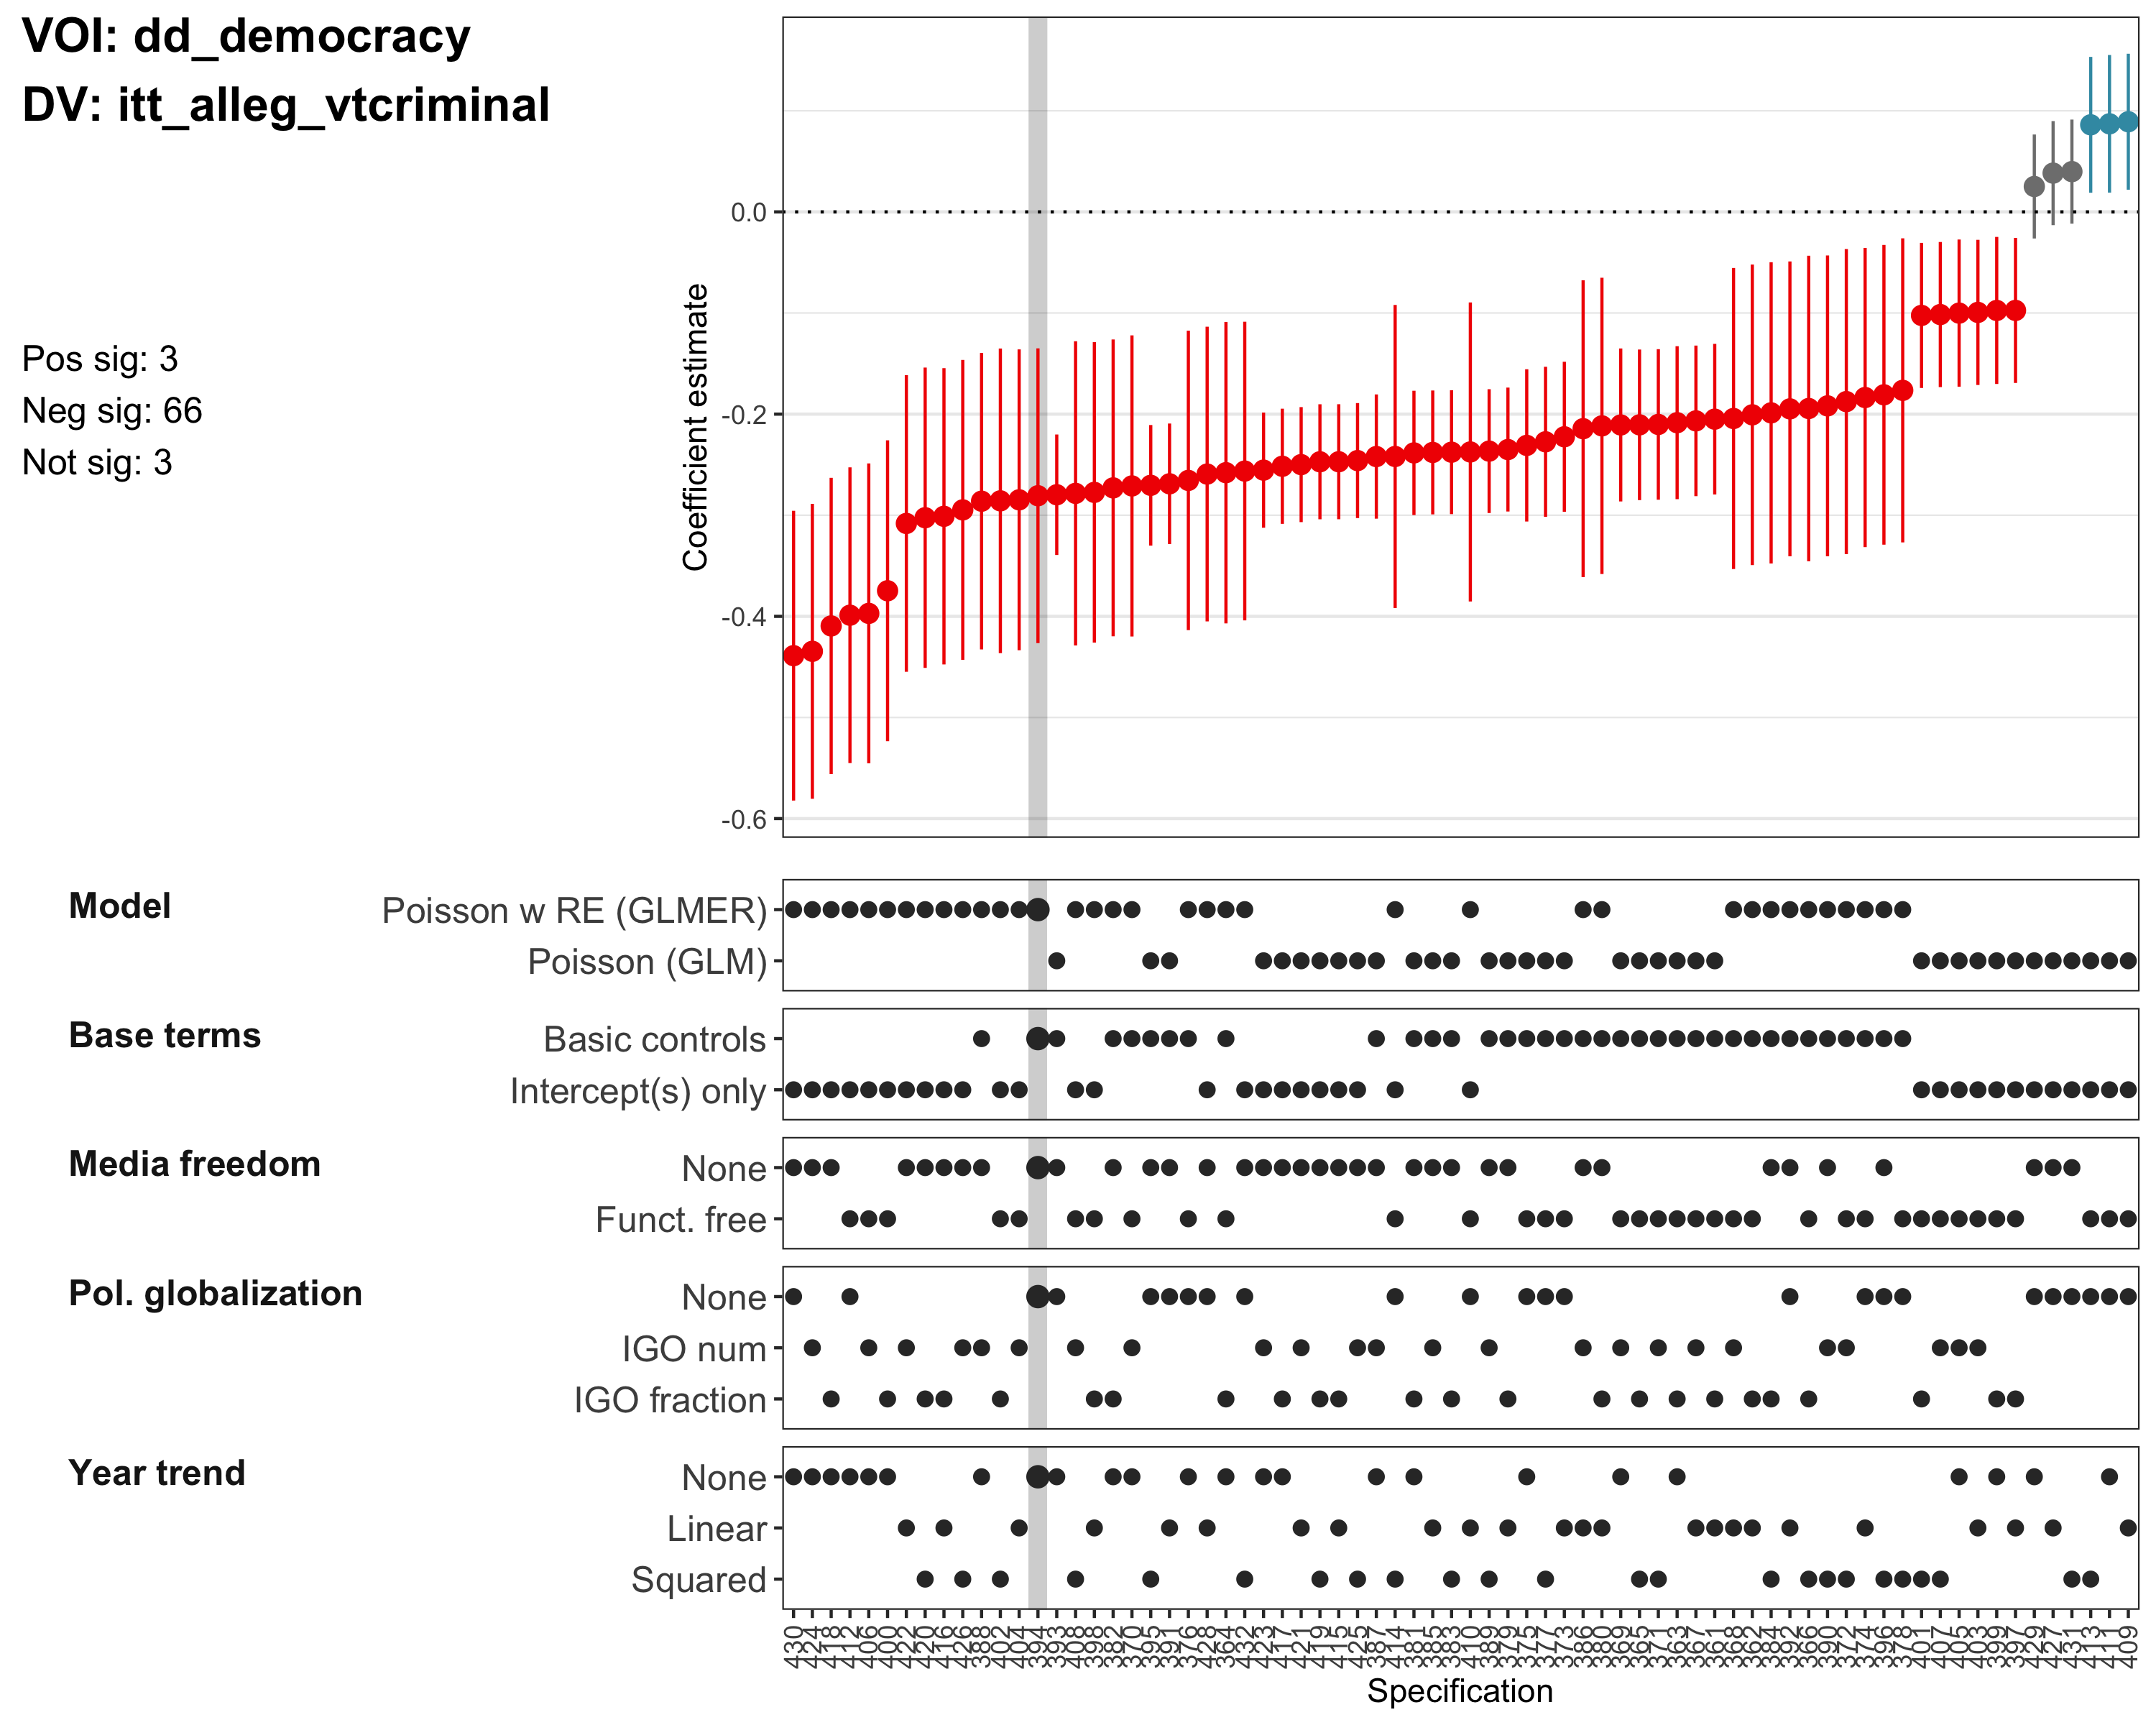
\includegraphics[height=4in]{../output/figures-robustness/specplot-dd_democracy-itt_alleg_vtcriminal.png}

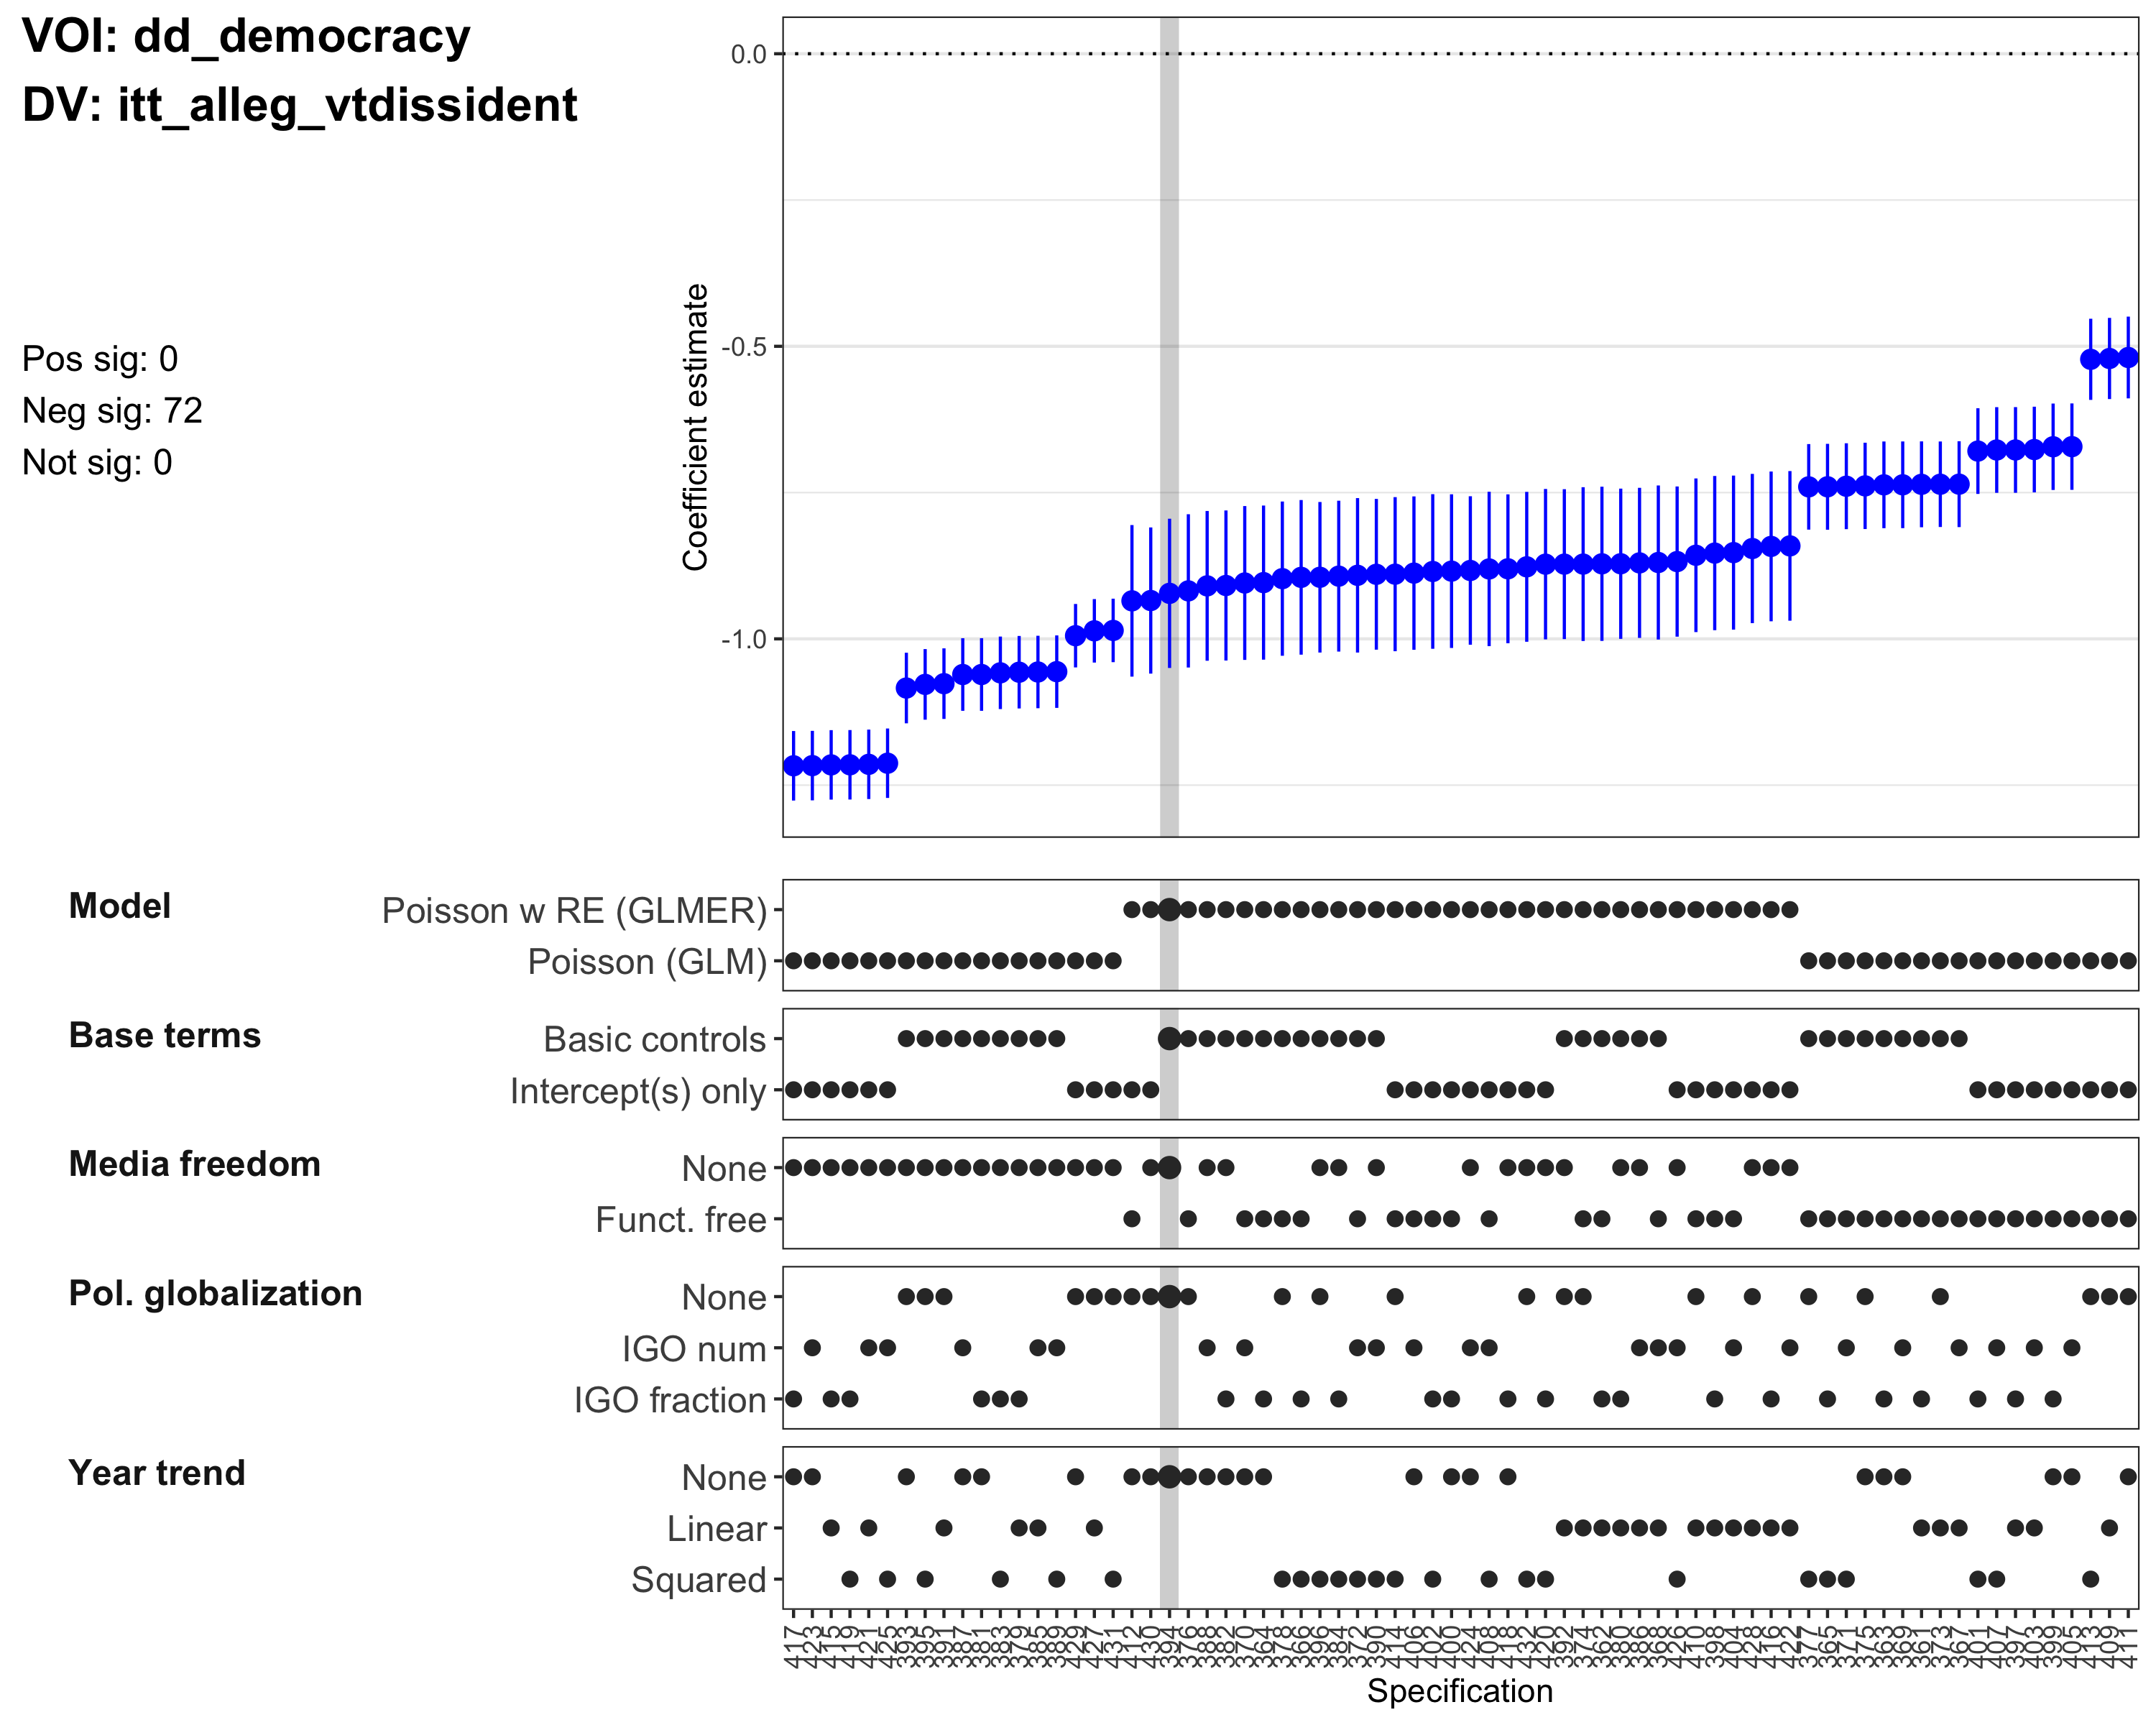
\includegraphics[height=4in]{../output/figures-robustness/specplot-dd_democracy-itt_alleg_vtdissident.png}

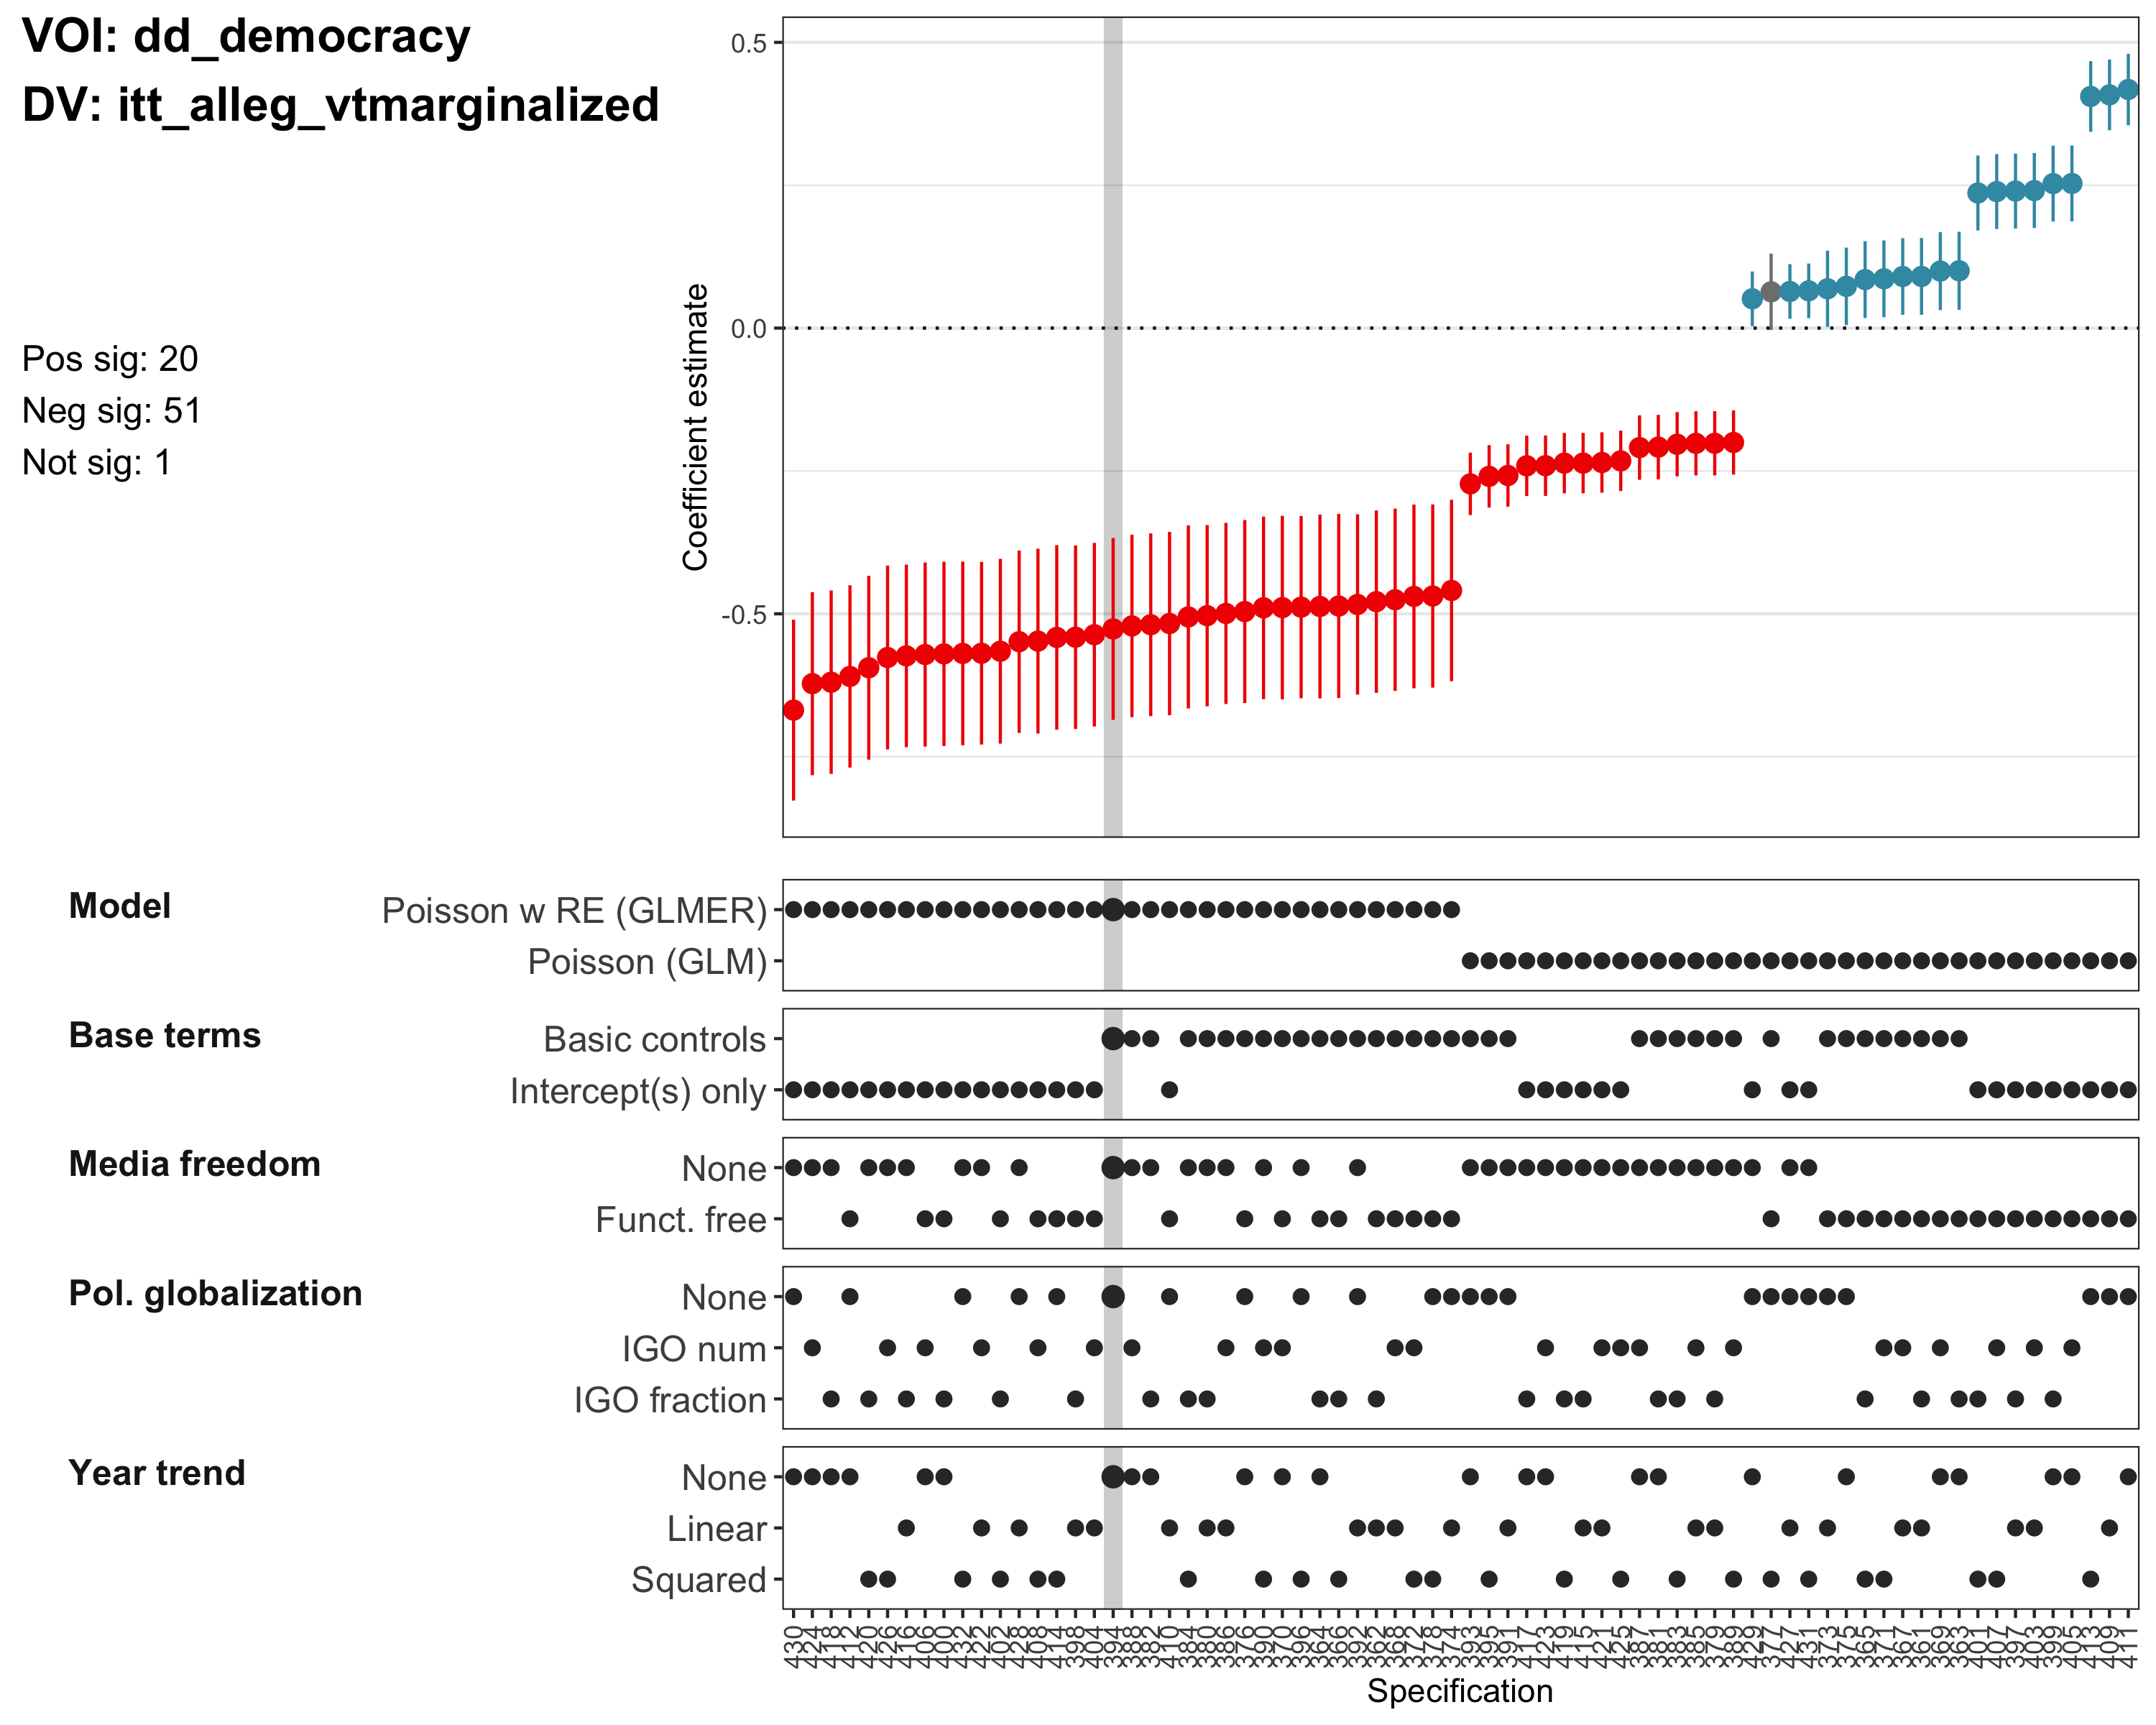
\includegraphics[height=4in]{../output/figures-robustness/specplot-dd_democracy-itt_alleg_vtmarginalized.png}

\hypertarget{voi-epr_excluded_group_pop}{%
\subsection{VOI:
epr\_excluded\_group\_pop}\label{voi-epr_excluded_group_pop}}

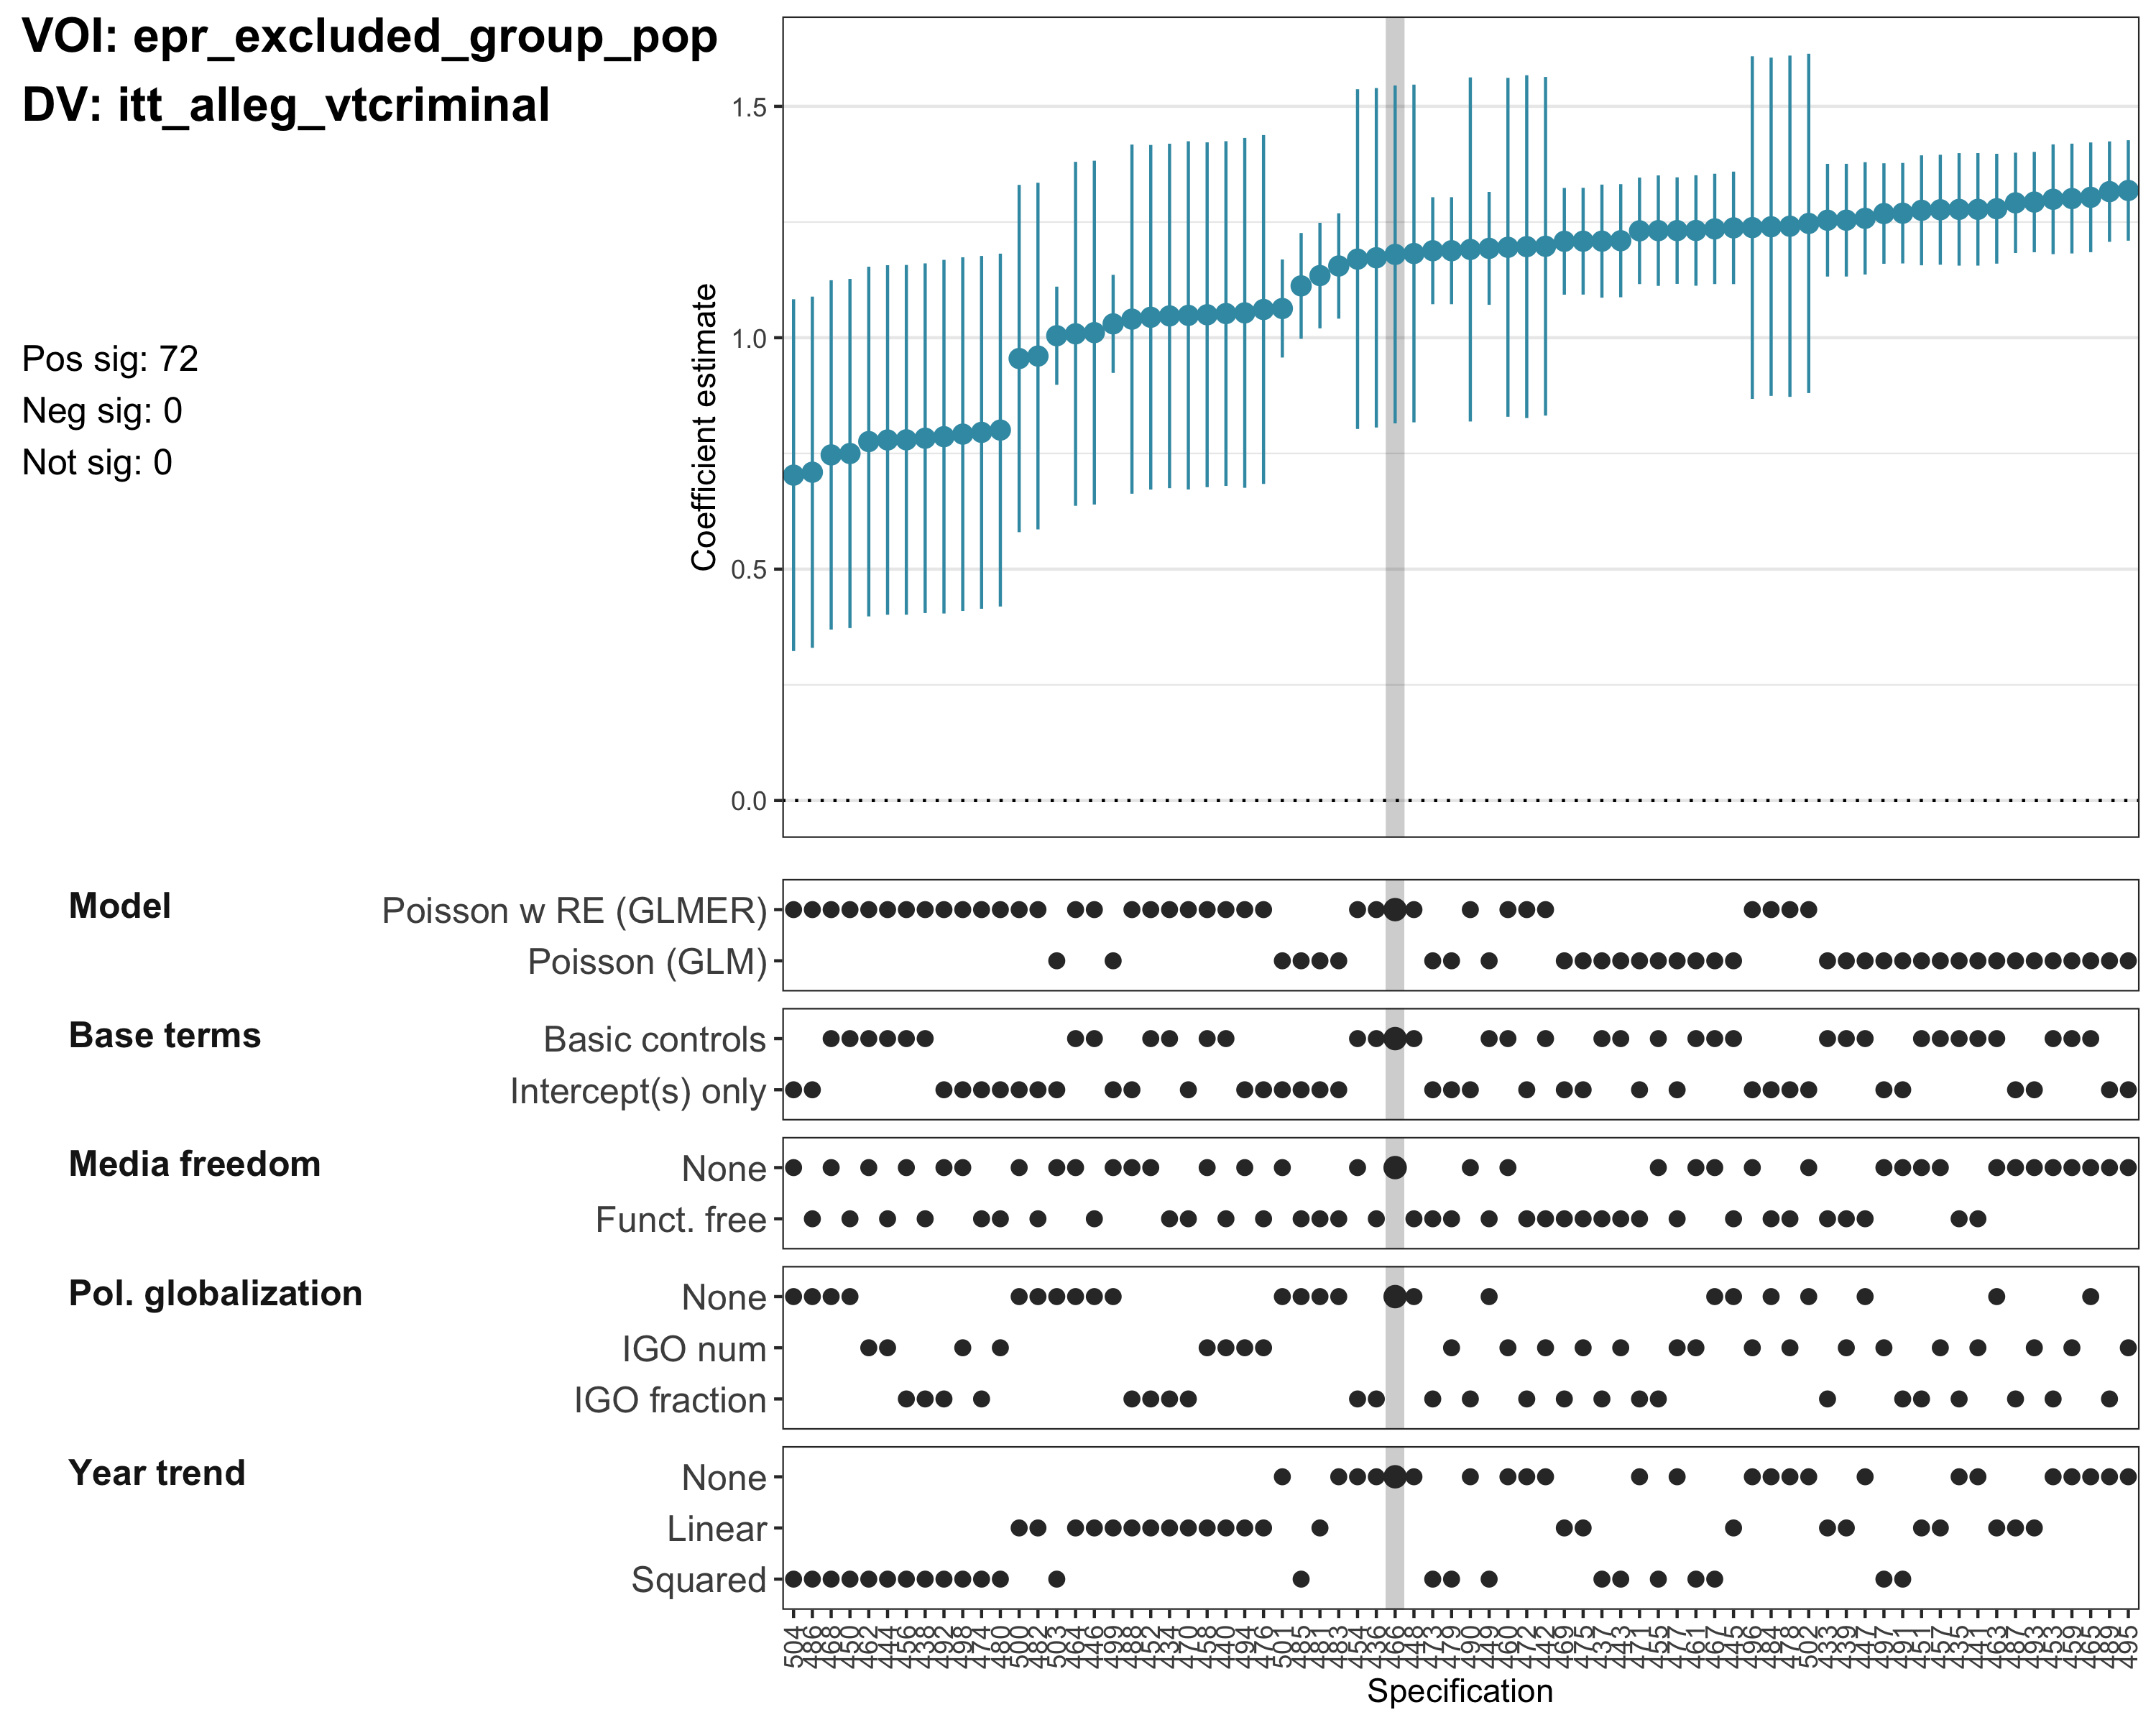
\includegraphics[height=4in]{../output/figures-robustness/specplot-epr_excluded_group_pop-itt_alleg_vtcriminal.png}

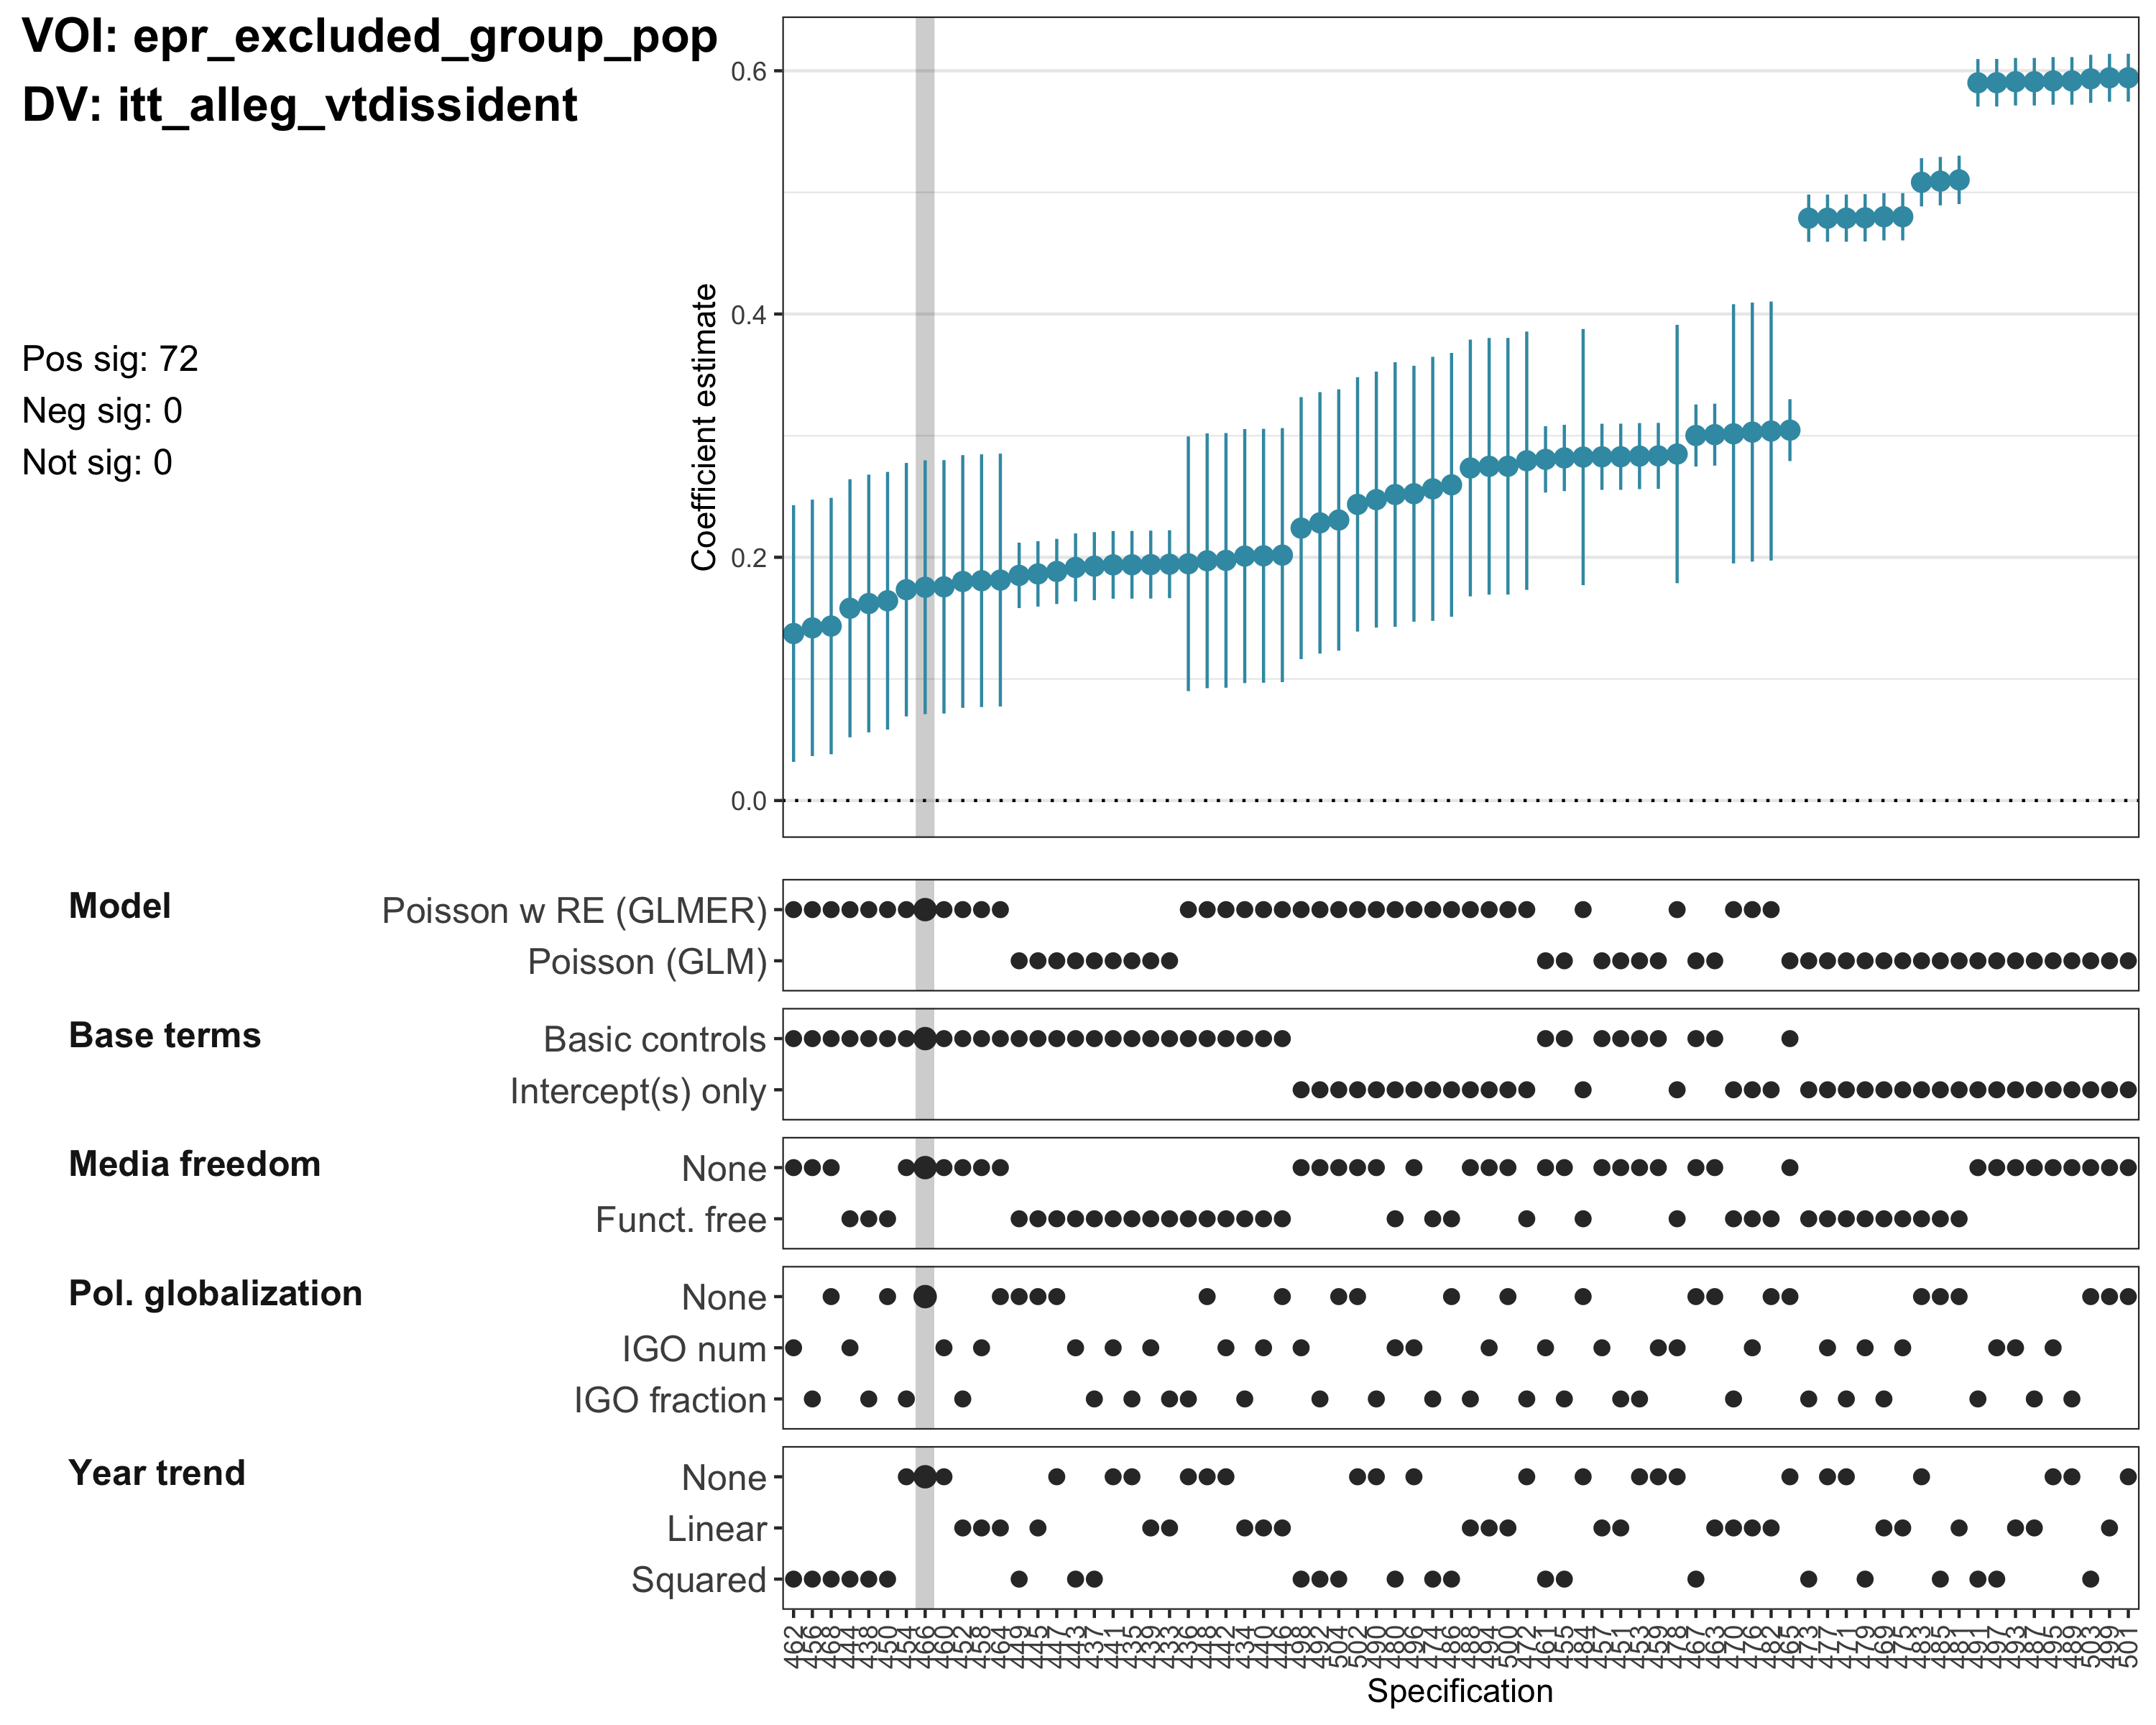
\includegraphics[height=4in]{../output/figures-robustness/specplot-epr_excluded_group_pop-itt_alleg_vtdissident.png}

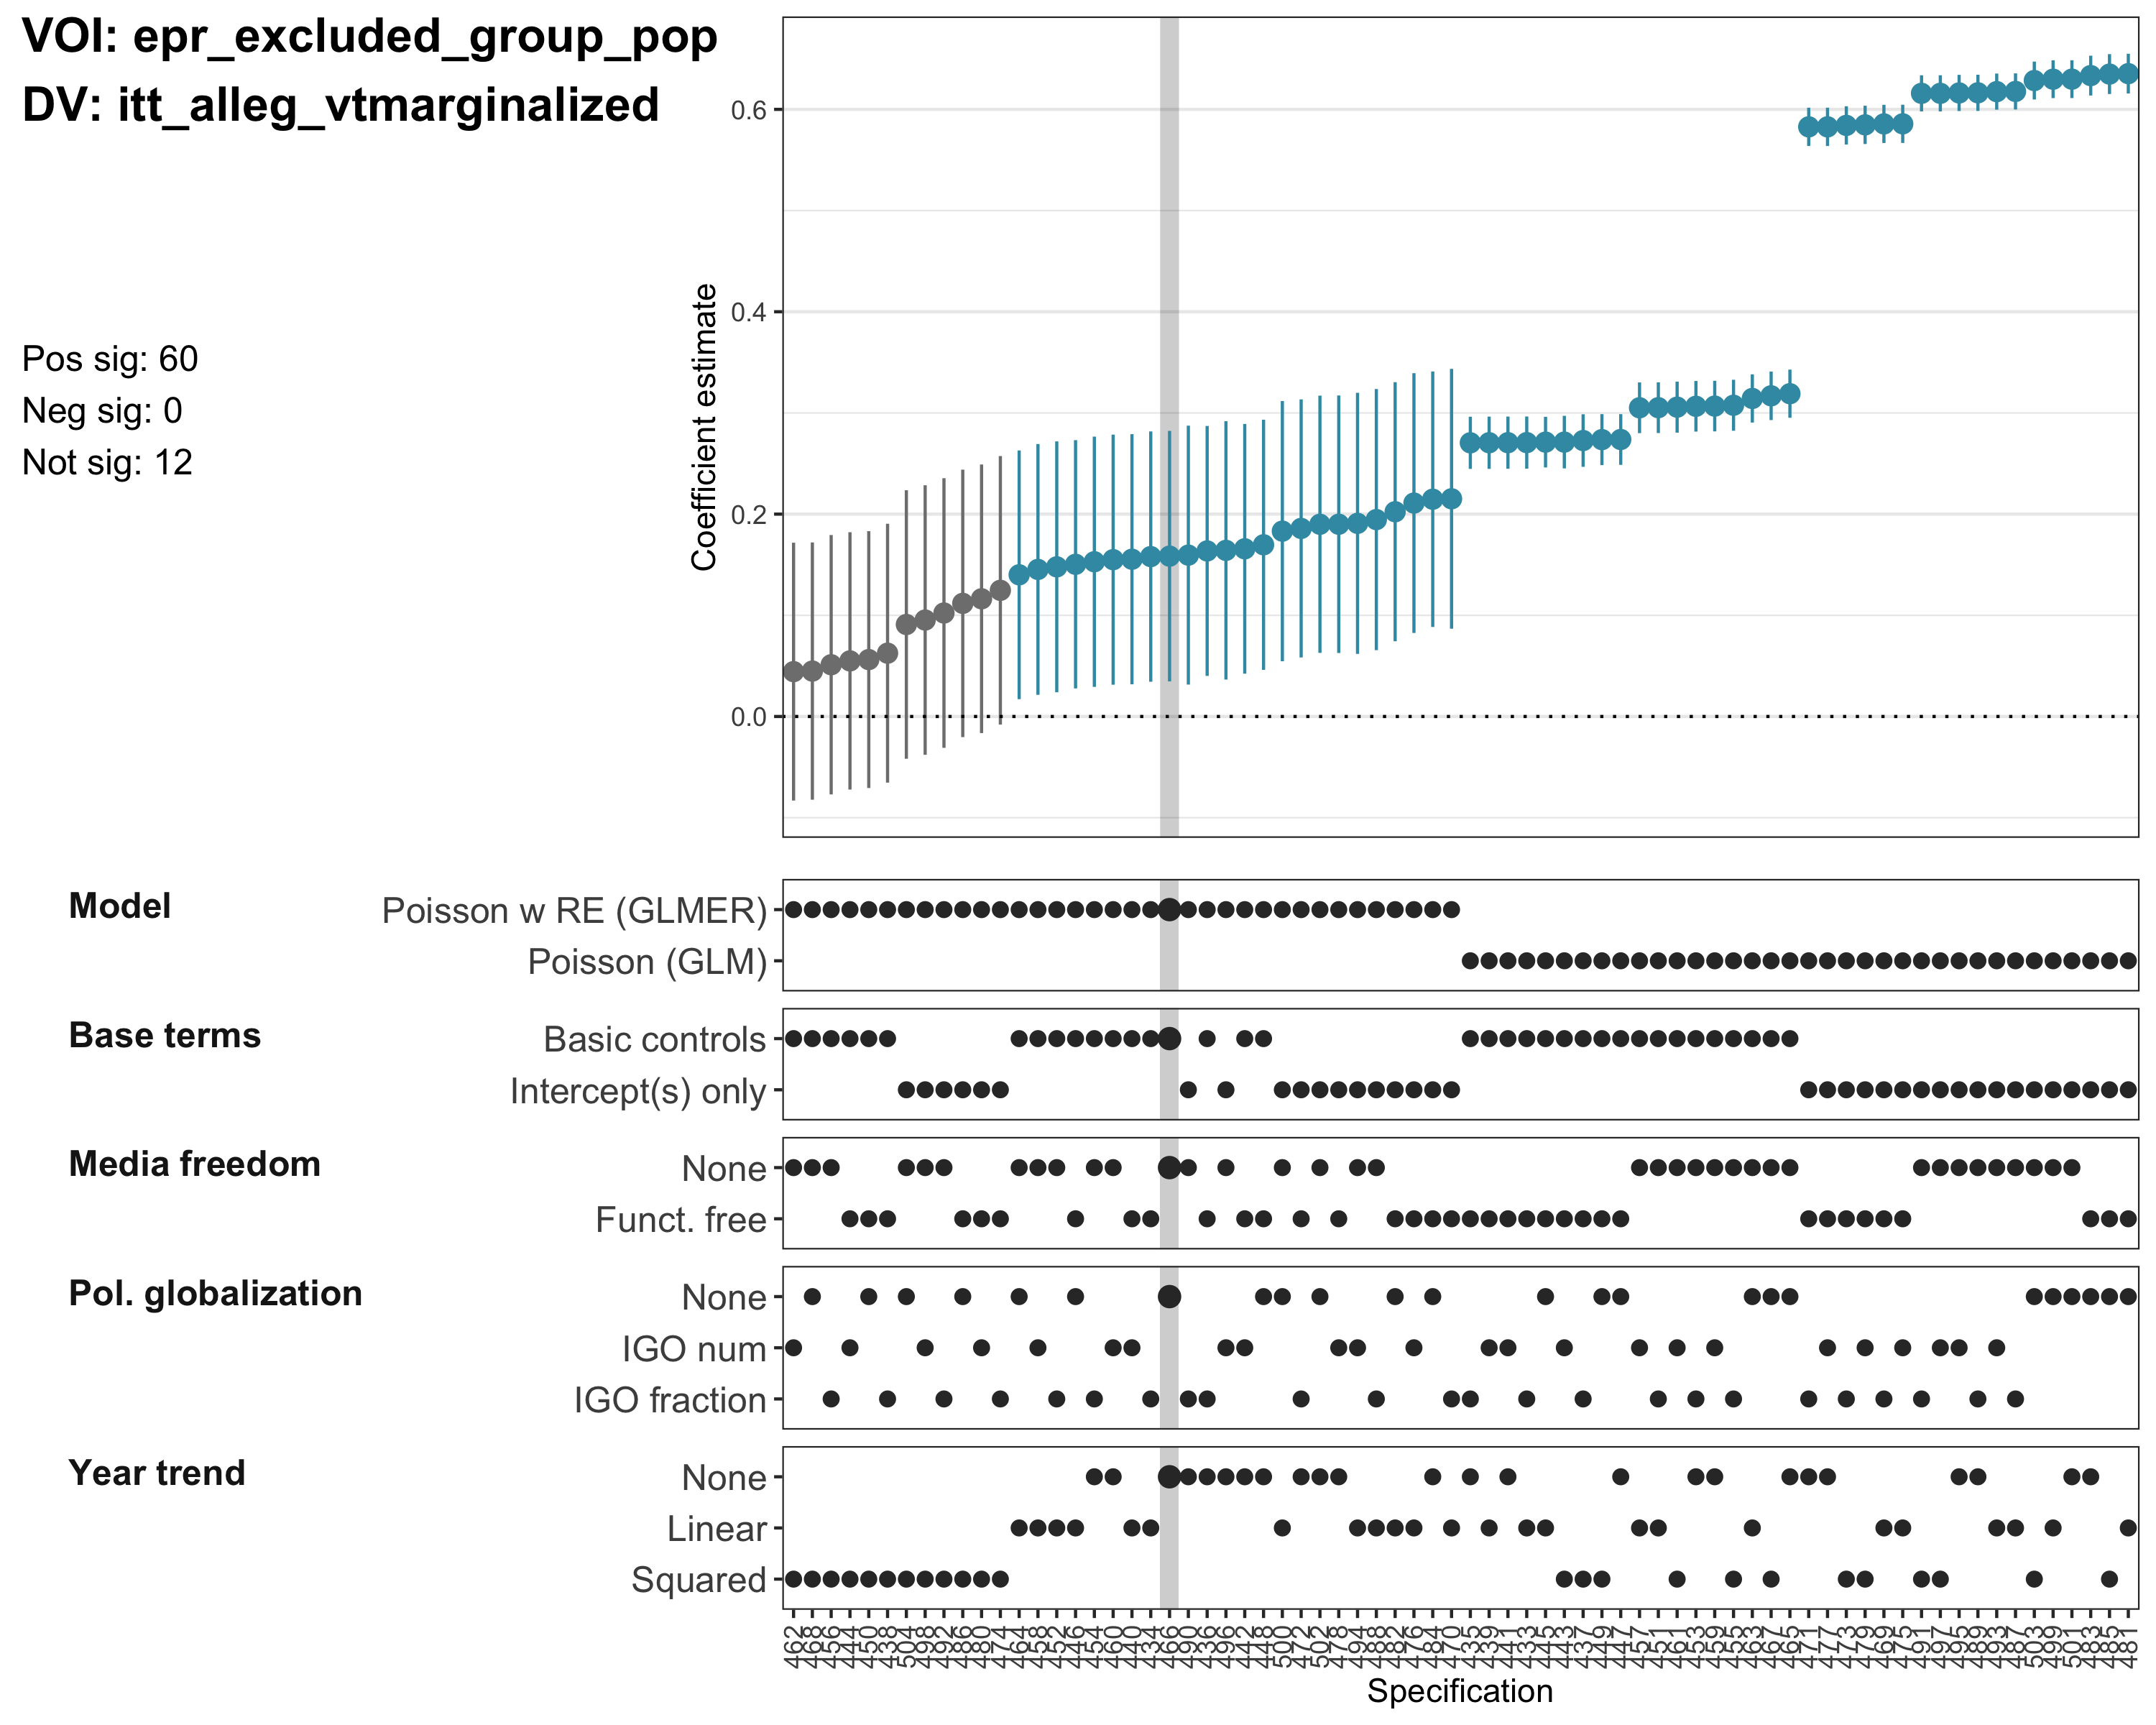
\includegraphics[height=4in]{../output/figures-robustness/specplot-epr_excluded_group_pop-itt_alleg_vtmarginalized.png}

\hypertarget{voi-epr_excluded_groups_count}{%
\subsection{VOI:
epr\_excluded\_groups\_count}\label{voi-epr_excluded_groups_count}}

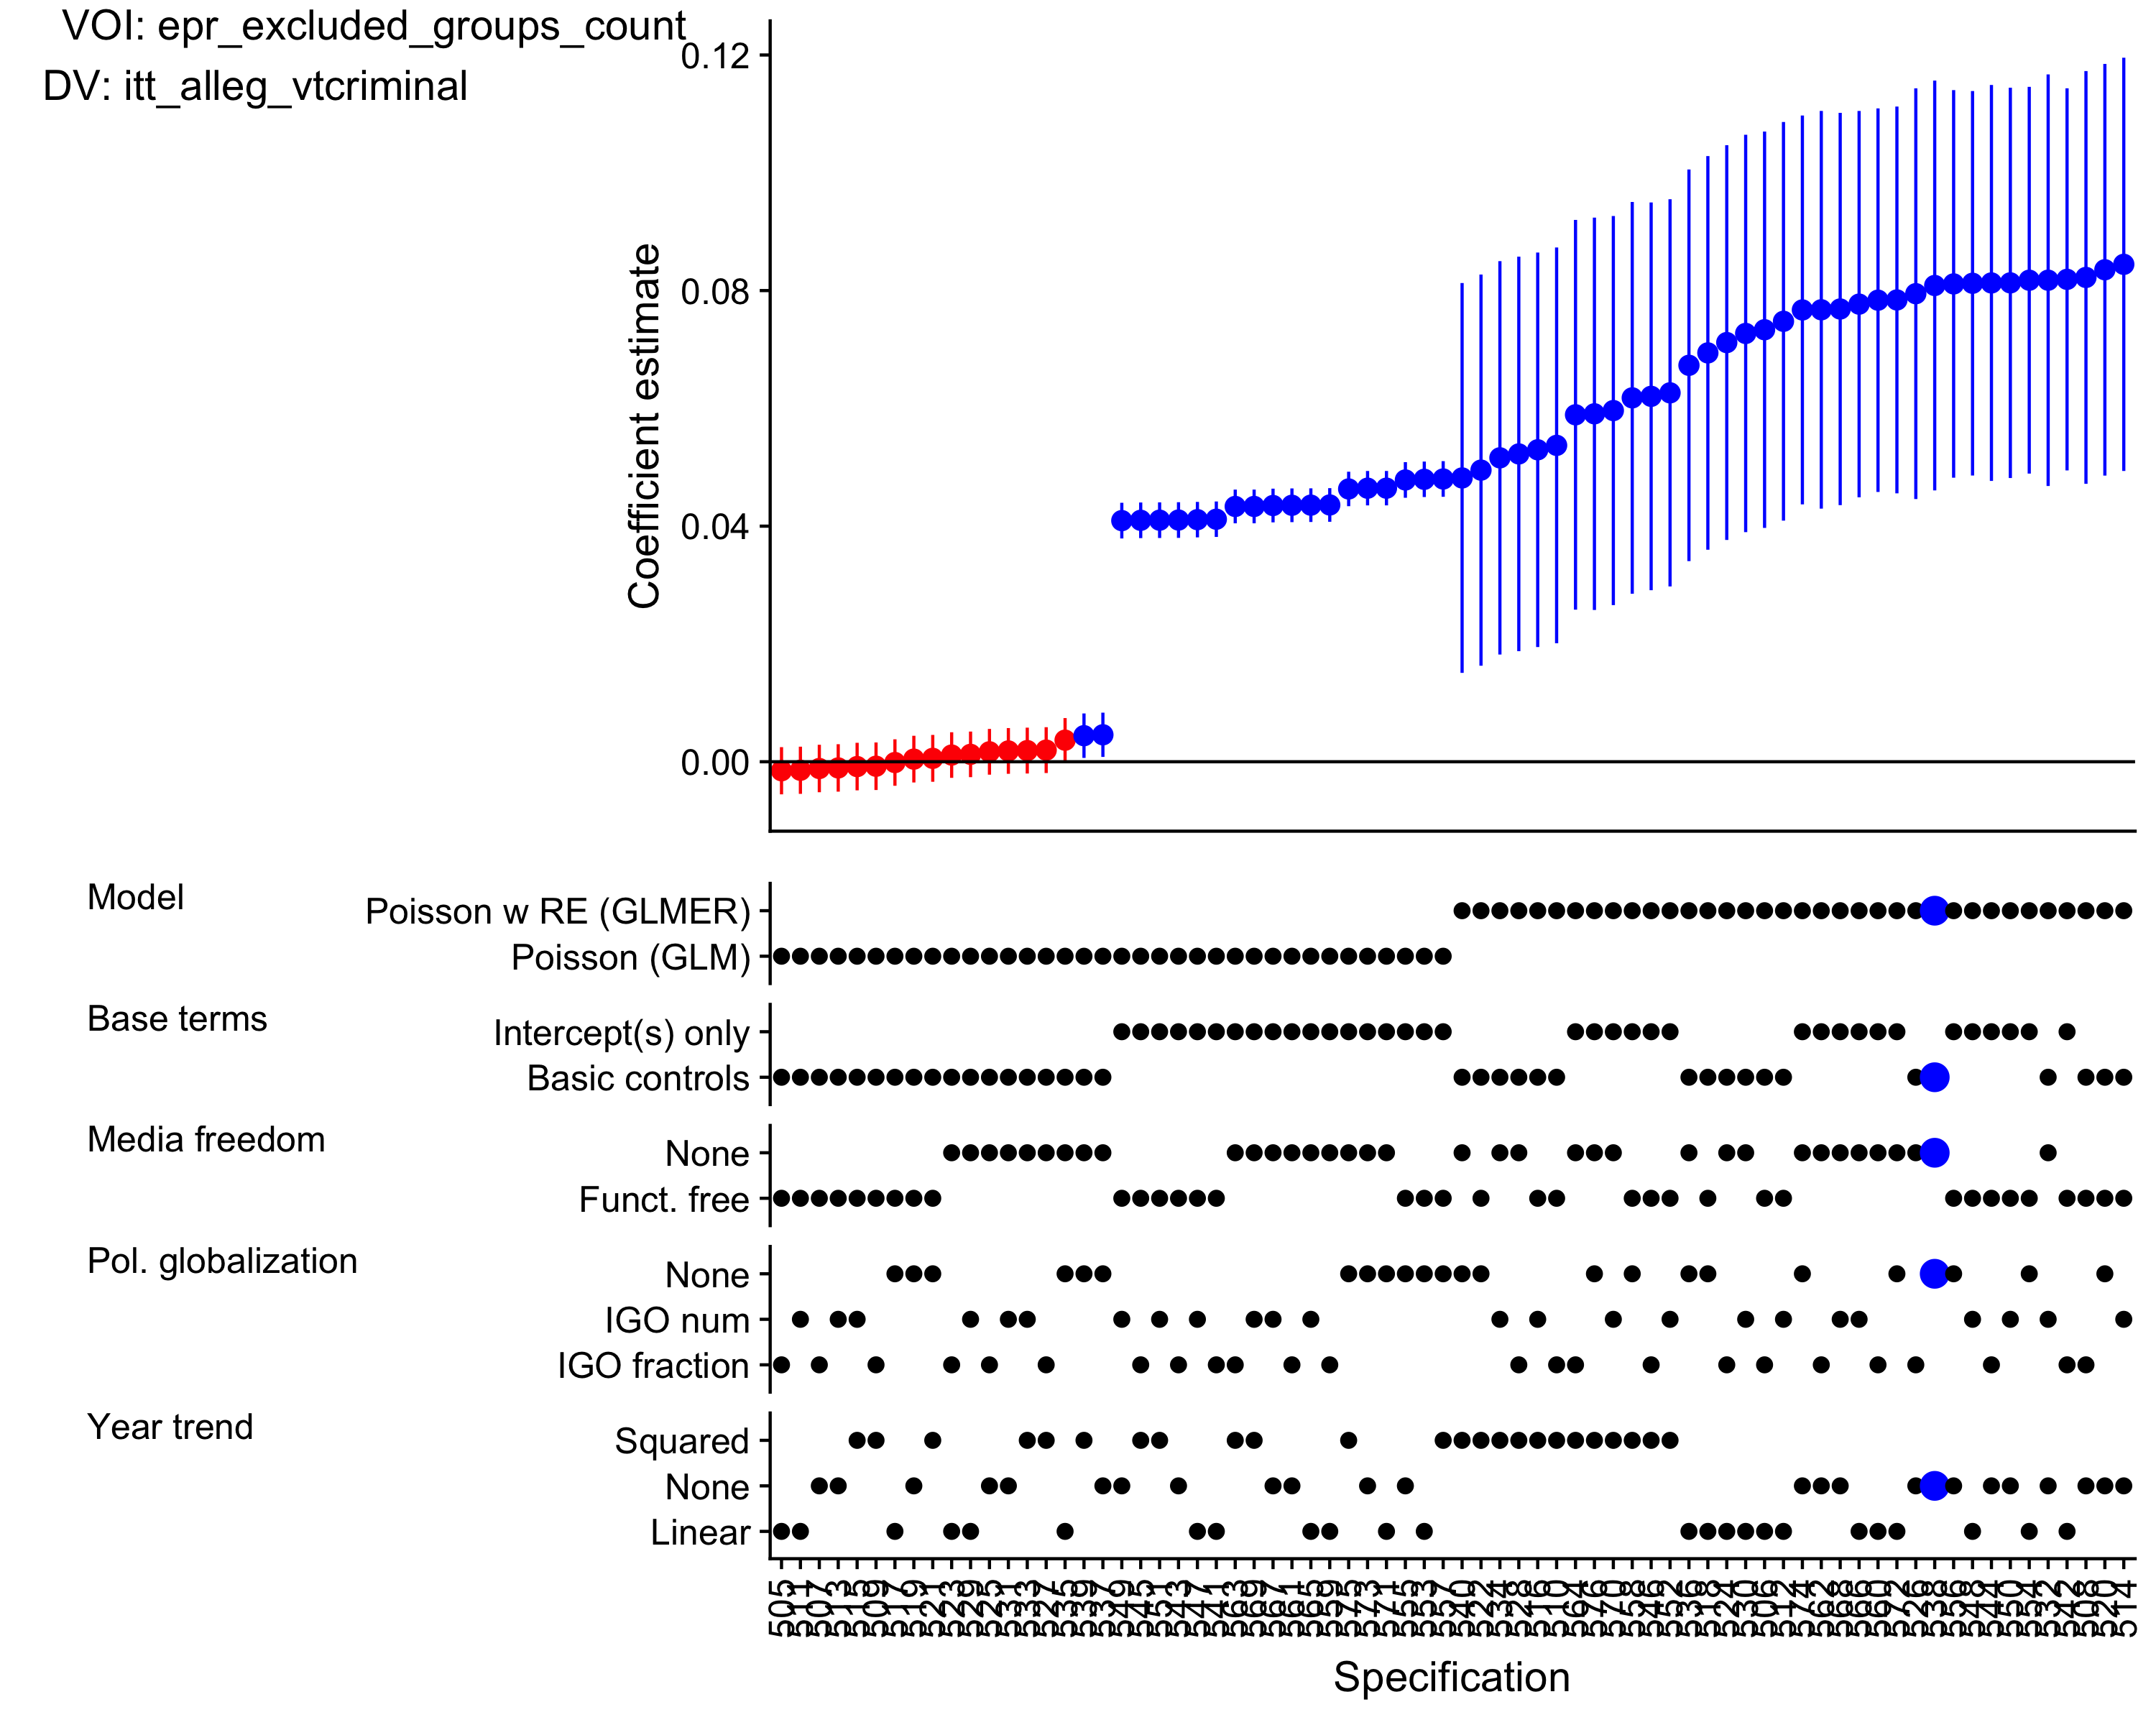
\includegraphics[height=4in]{../output/figures-robustness/specplot-epr_excluded_groups_count-itt_alleg_vtcriminal.png}

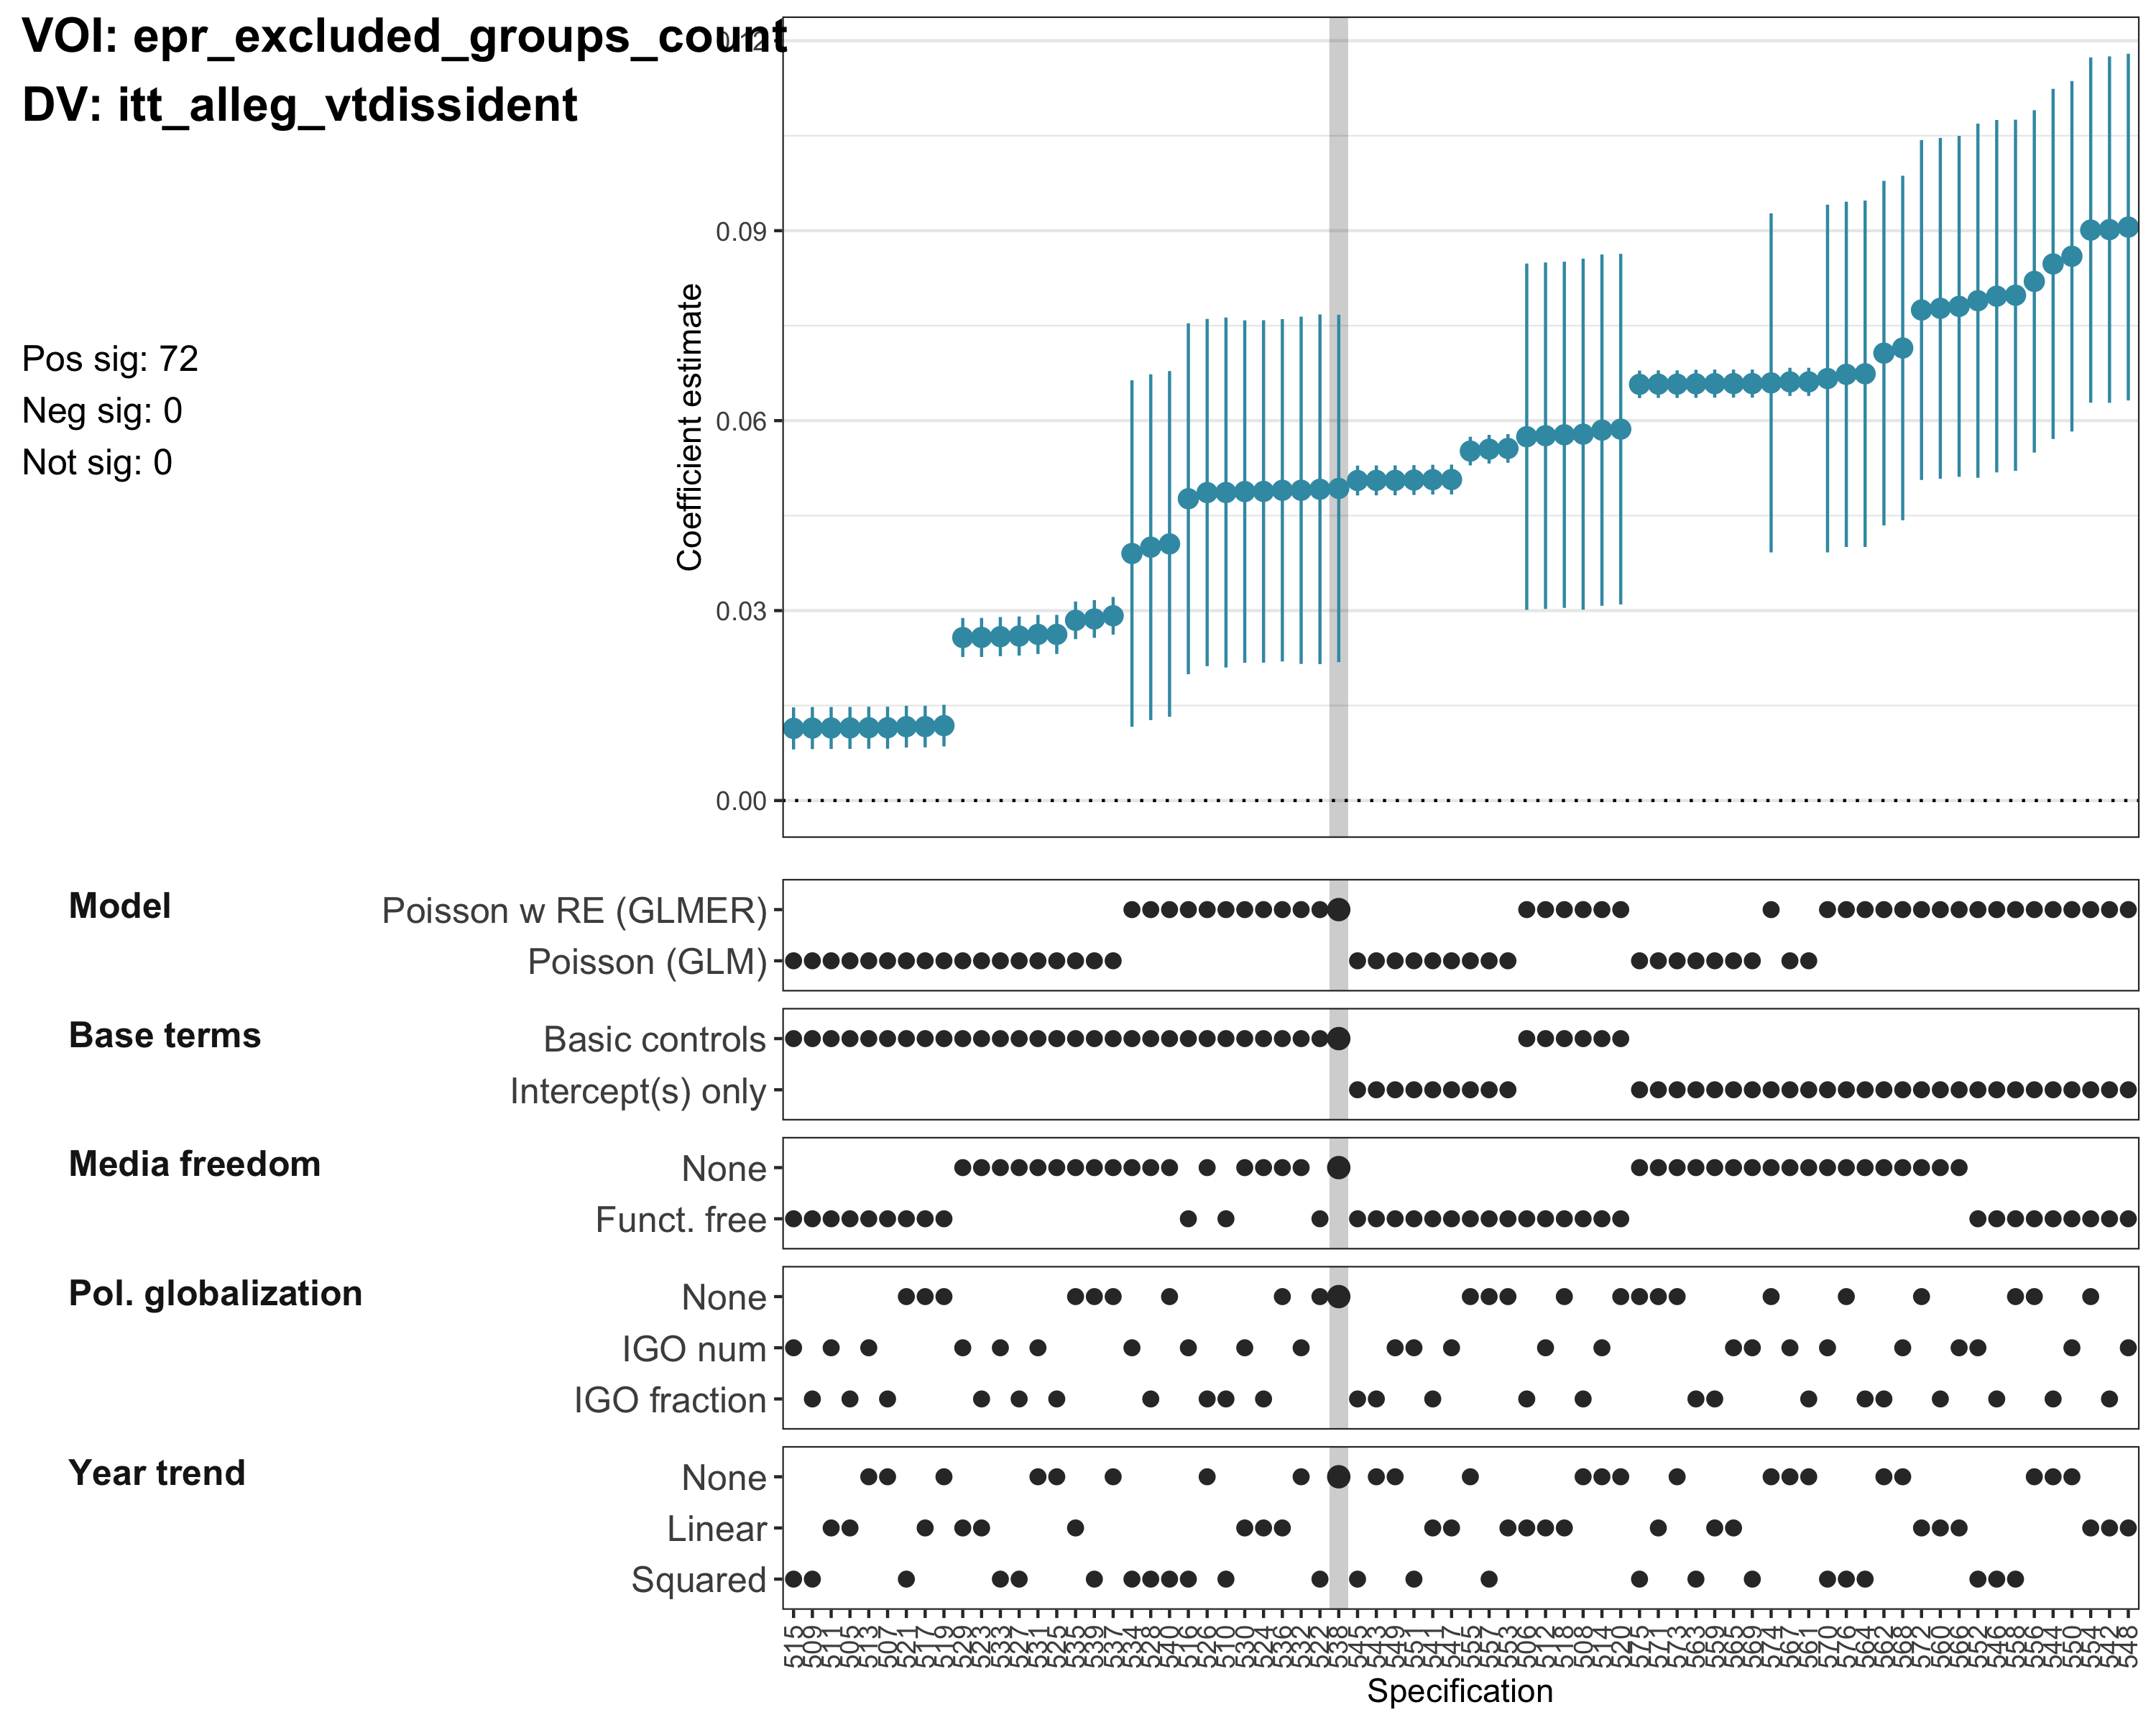
\includegraphics[height=4in]{../output/figures-robustness/specplot-epr_excluded_groups_count-itt_alleg_vtdissident.png}

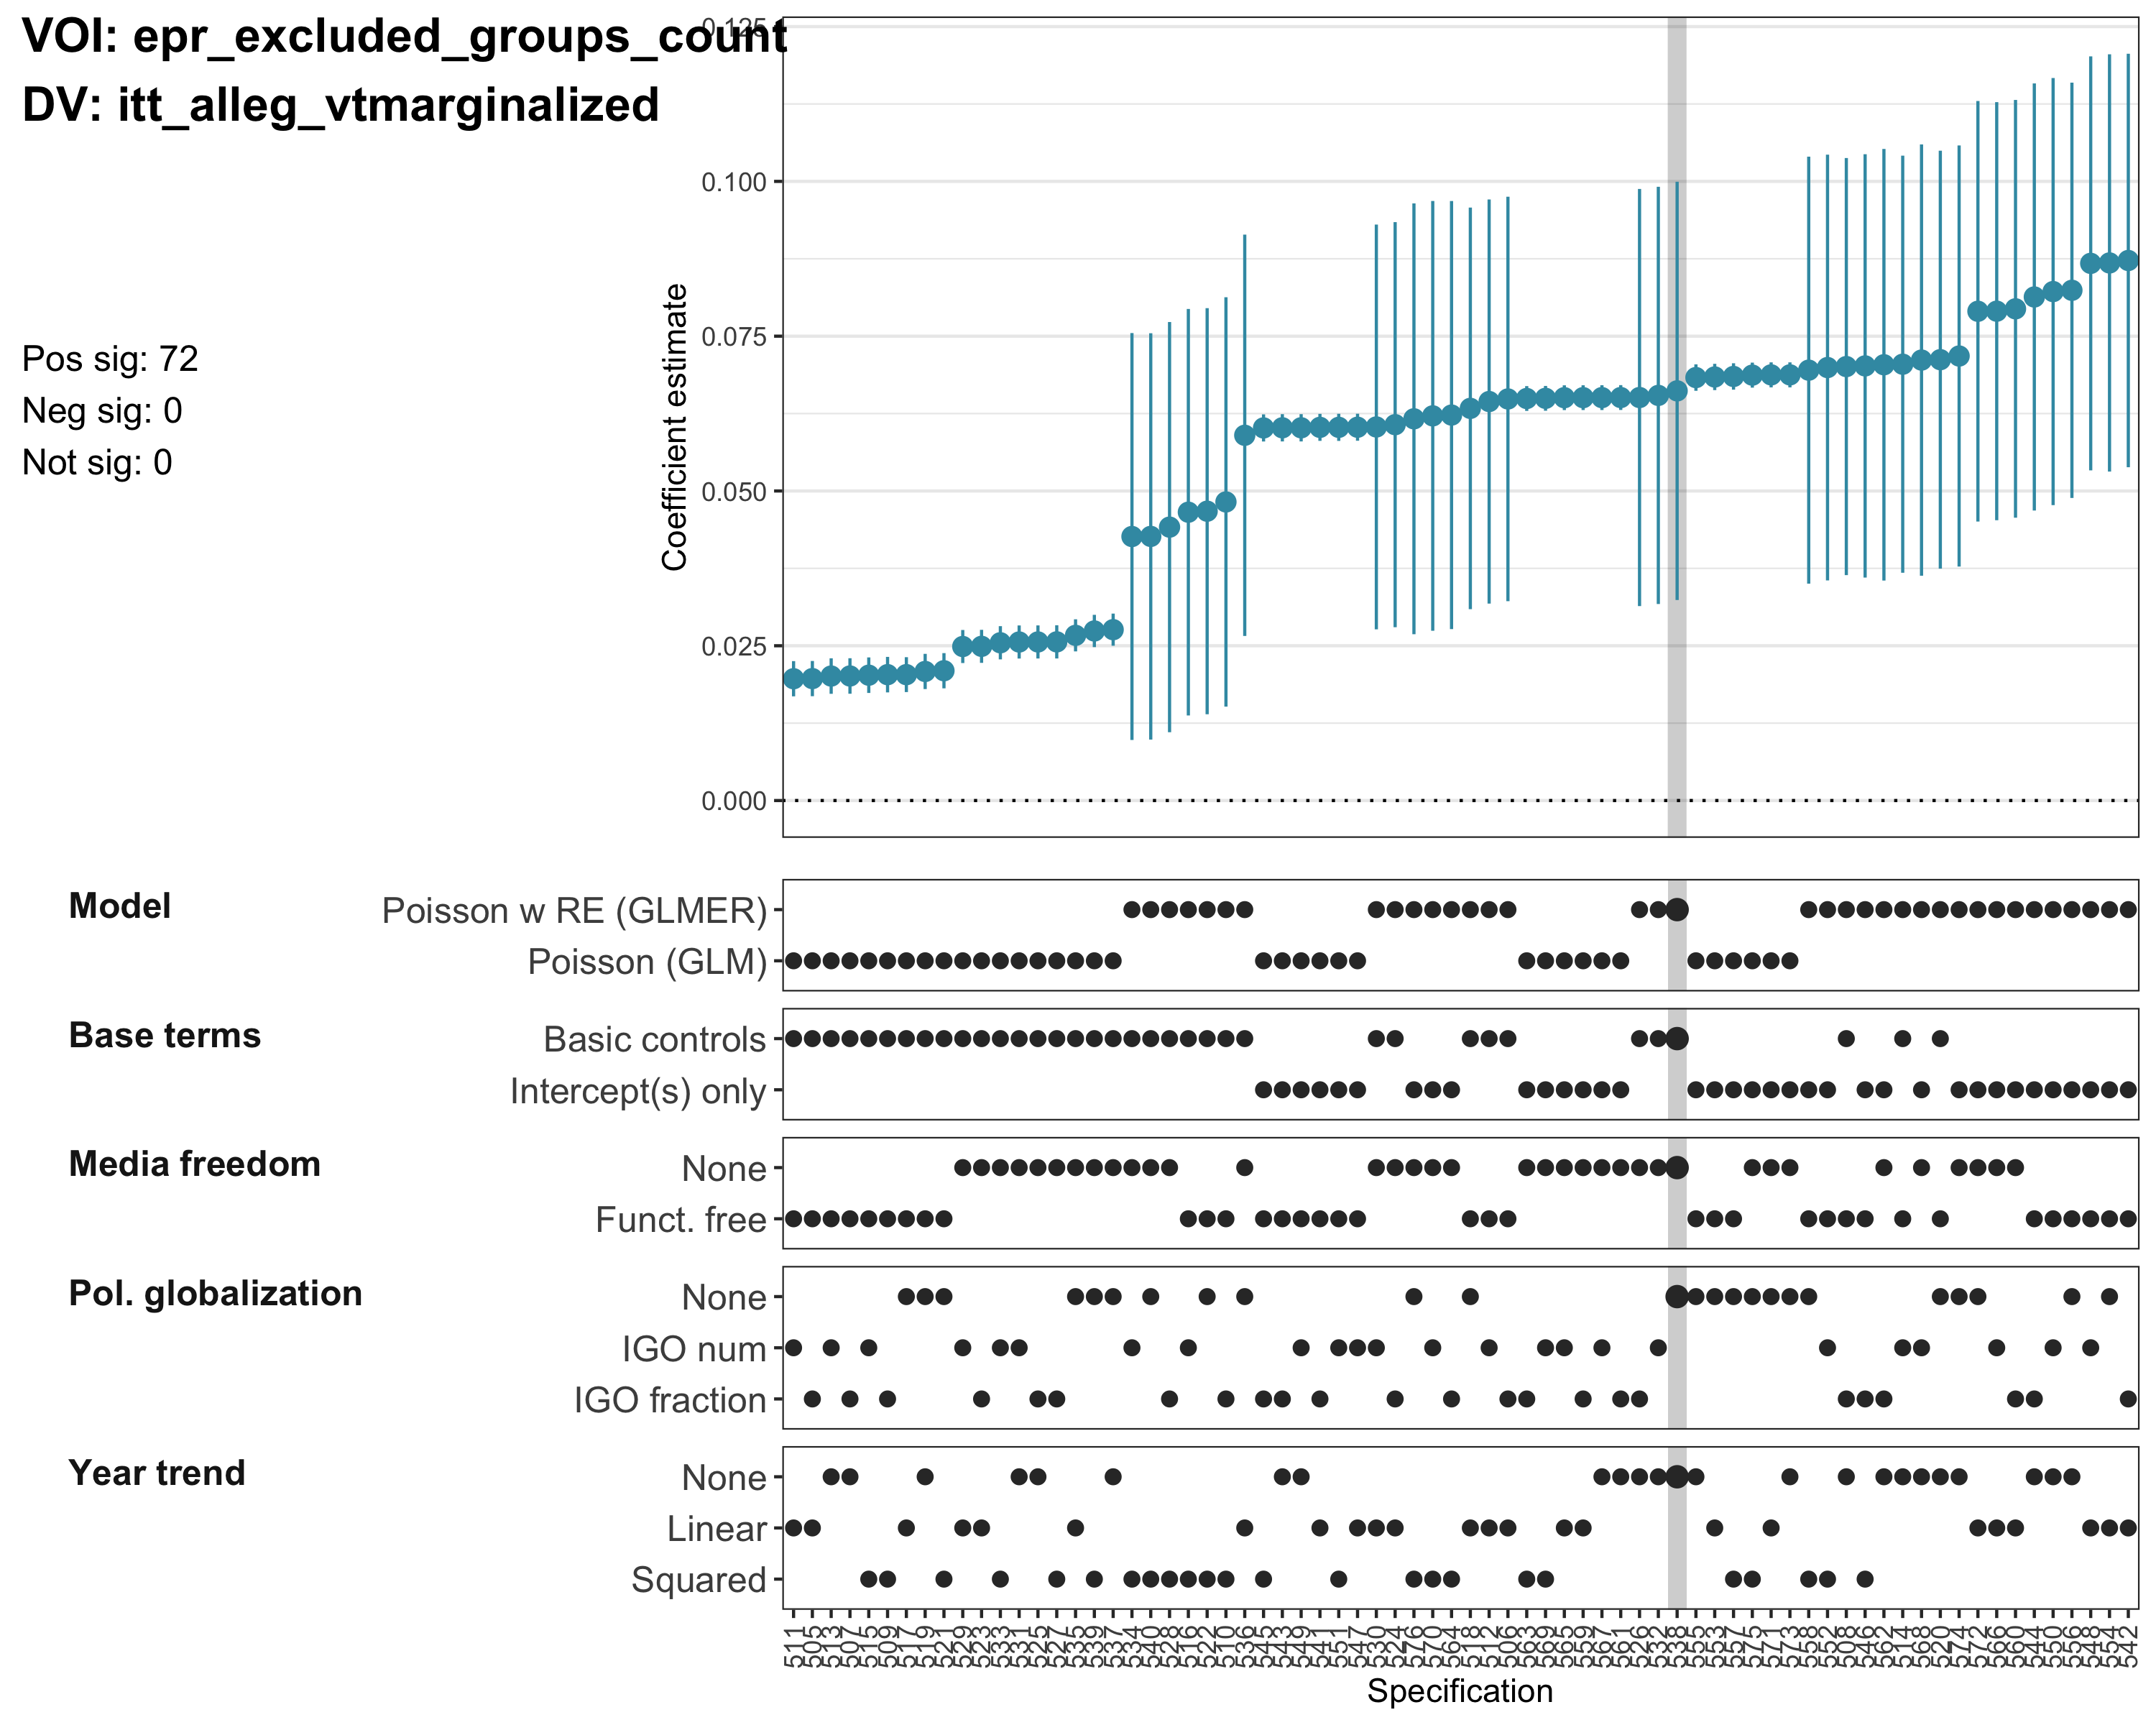
\includegraphics[height=4in]{../output/figures-robustness/specplot-epr_excluded_groups_count-itt_alleg_vtmarginalized.png}

\hypertarget{voi-v2clacjust}{%
\subsection{VOI: v2clacjust}\label{voi-v2clacjust}}

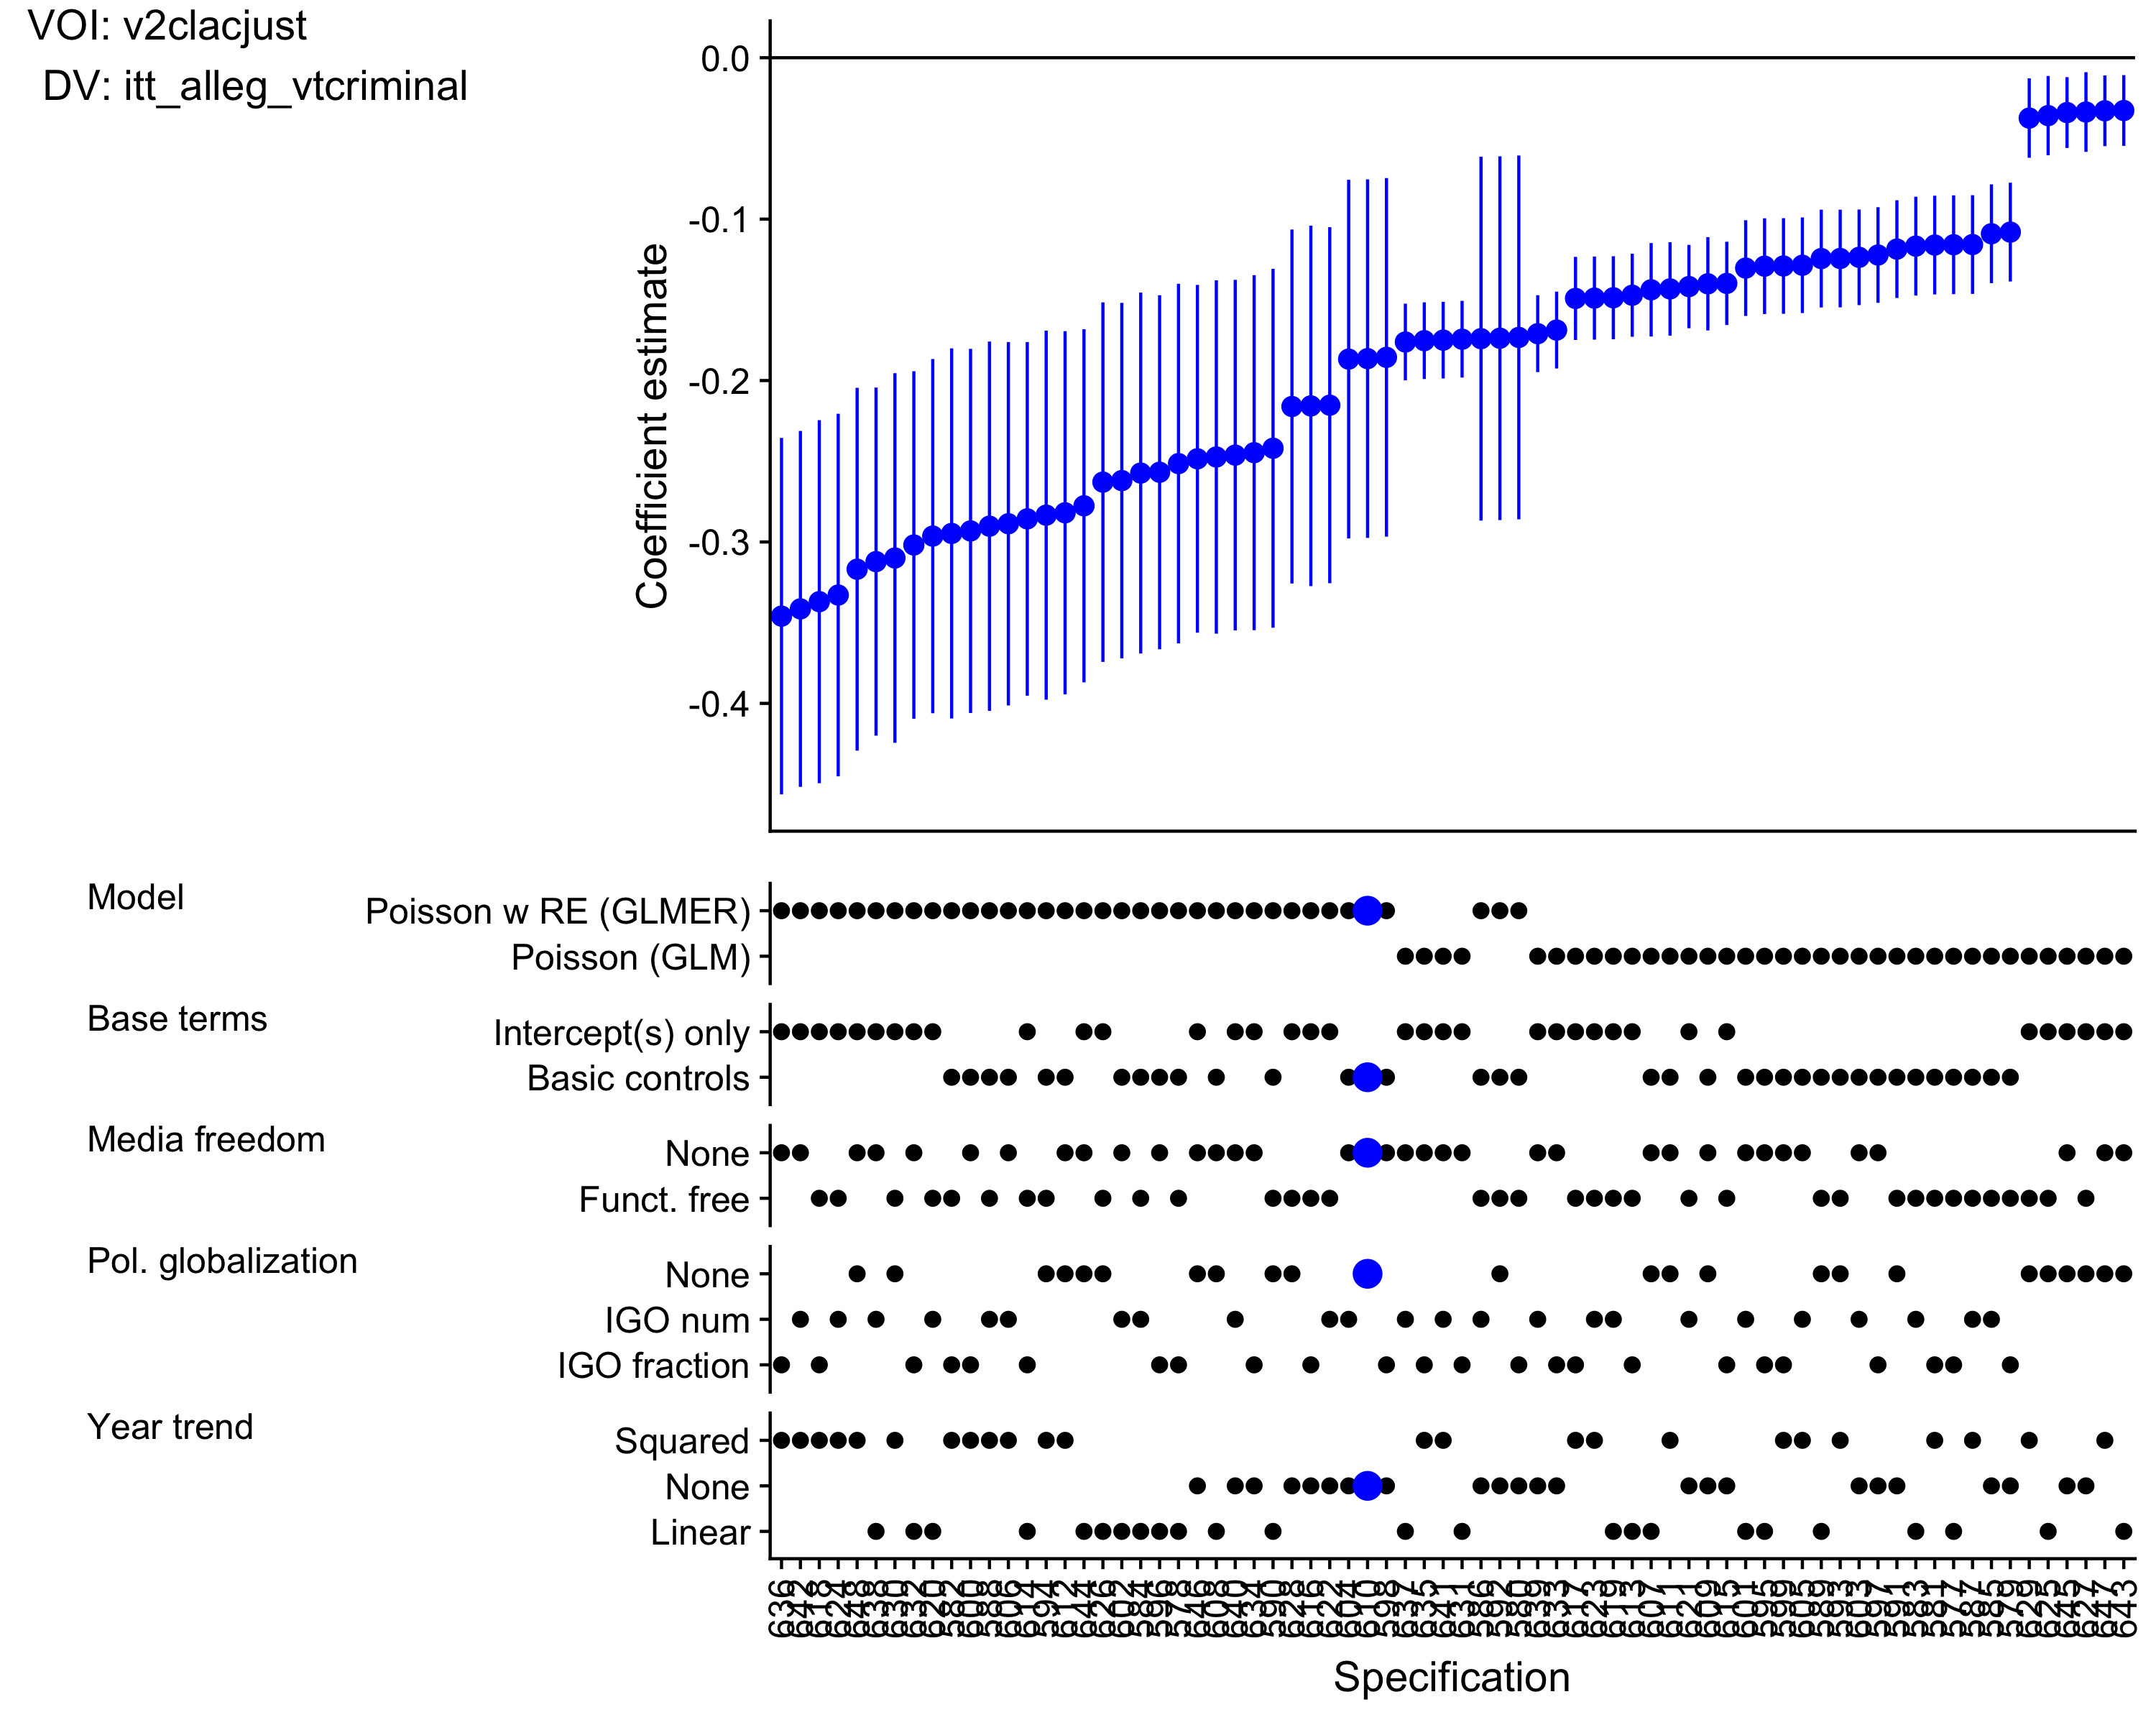
\includegraphics[height=4in]{../output/figures-robustness/specplot-v2clacjust-itt_alleg_vtcriminal.png}

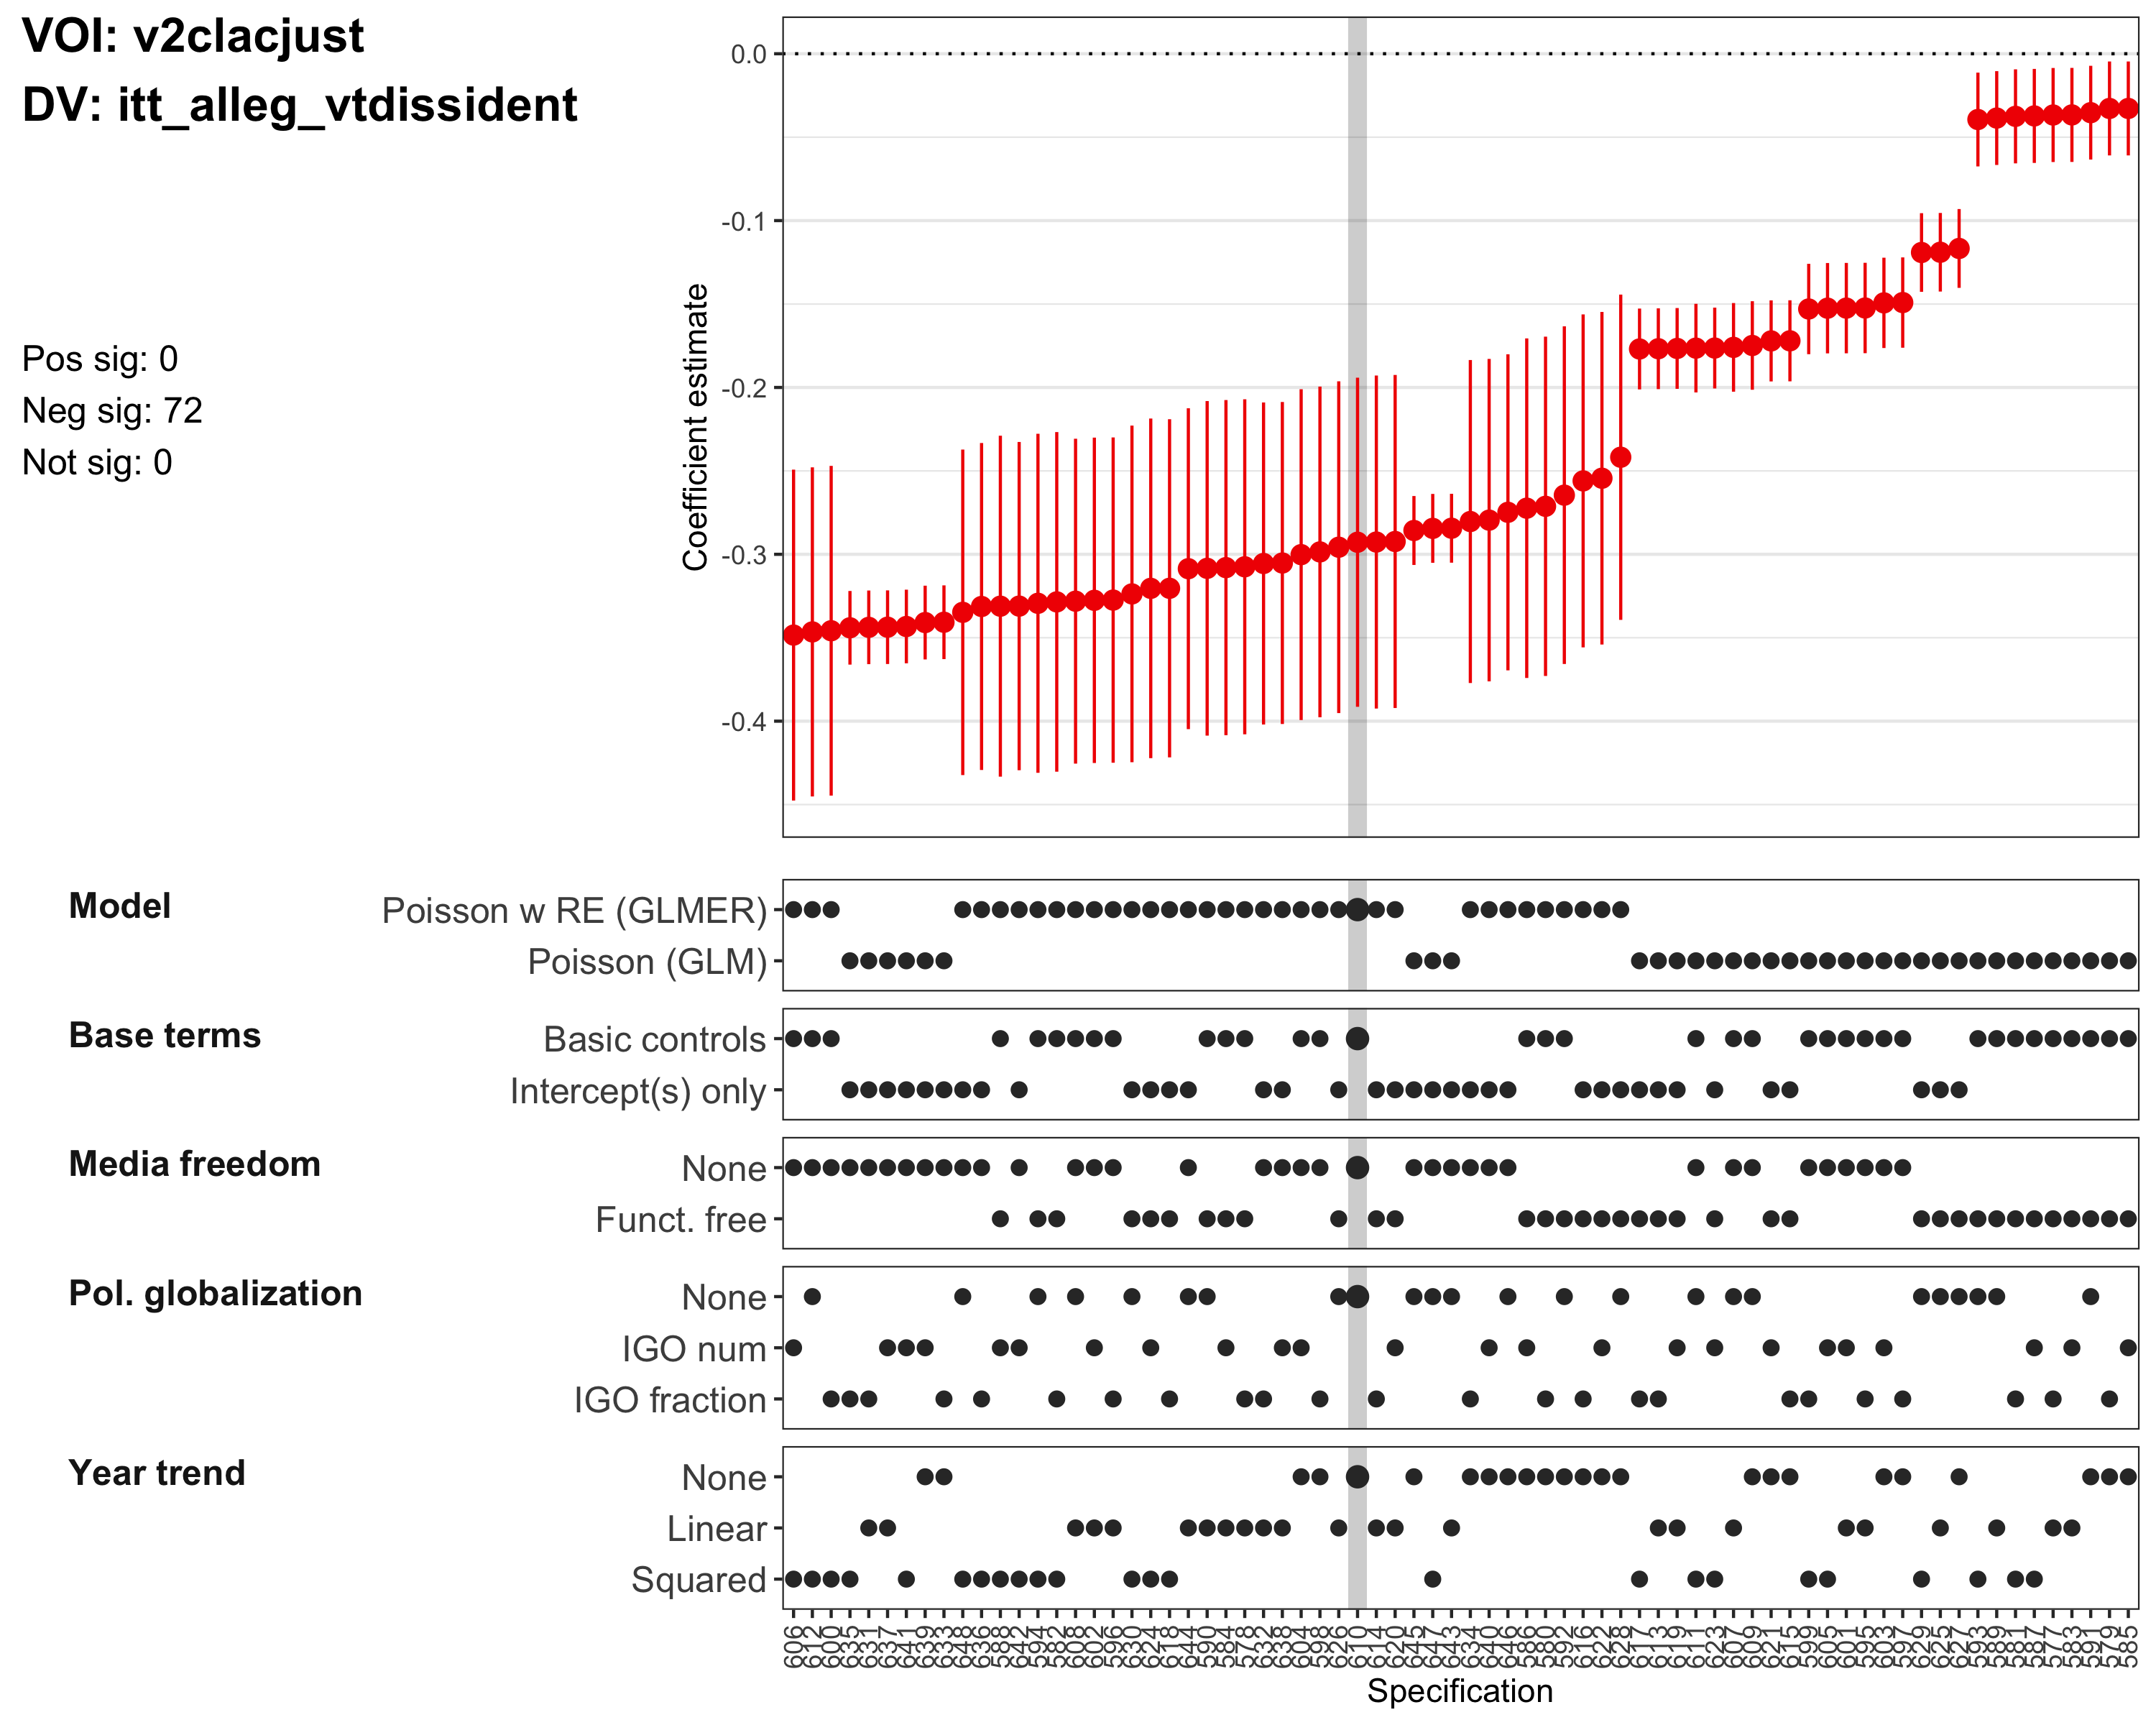
\includegraphics[height=4in]{../output/figures-robustness/specplot-v2clacjust-itt_alleg_vtdissident.png}

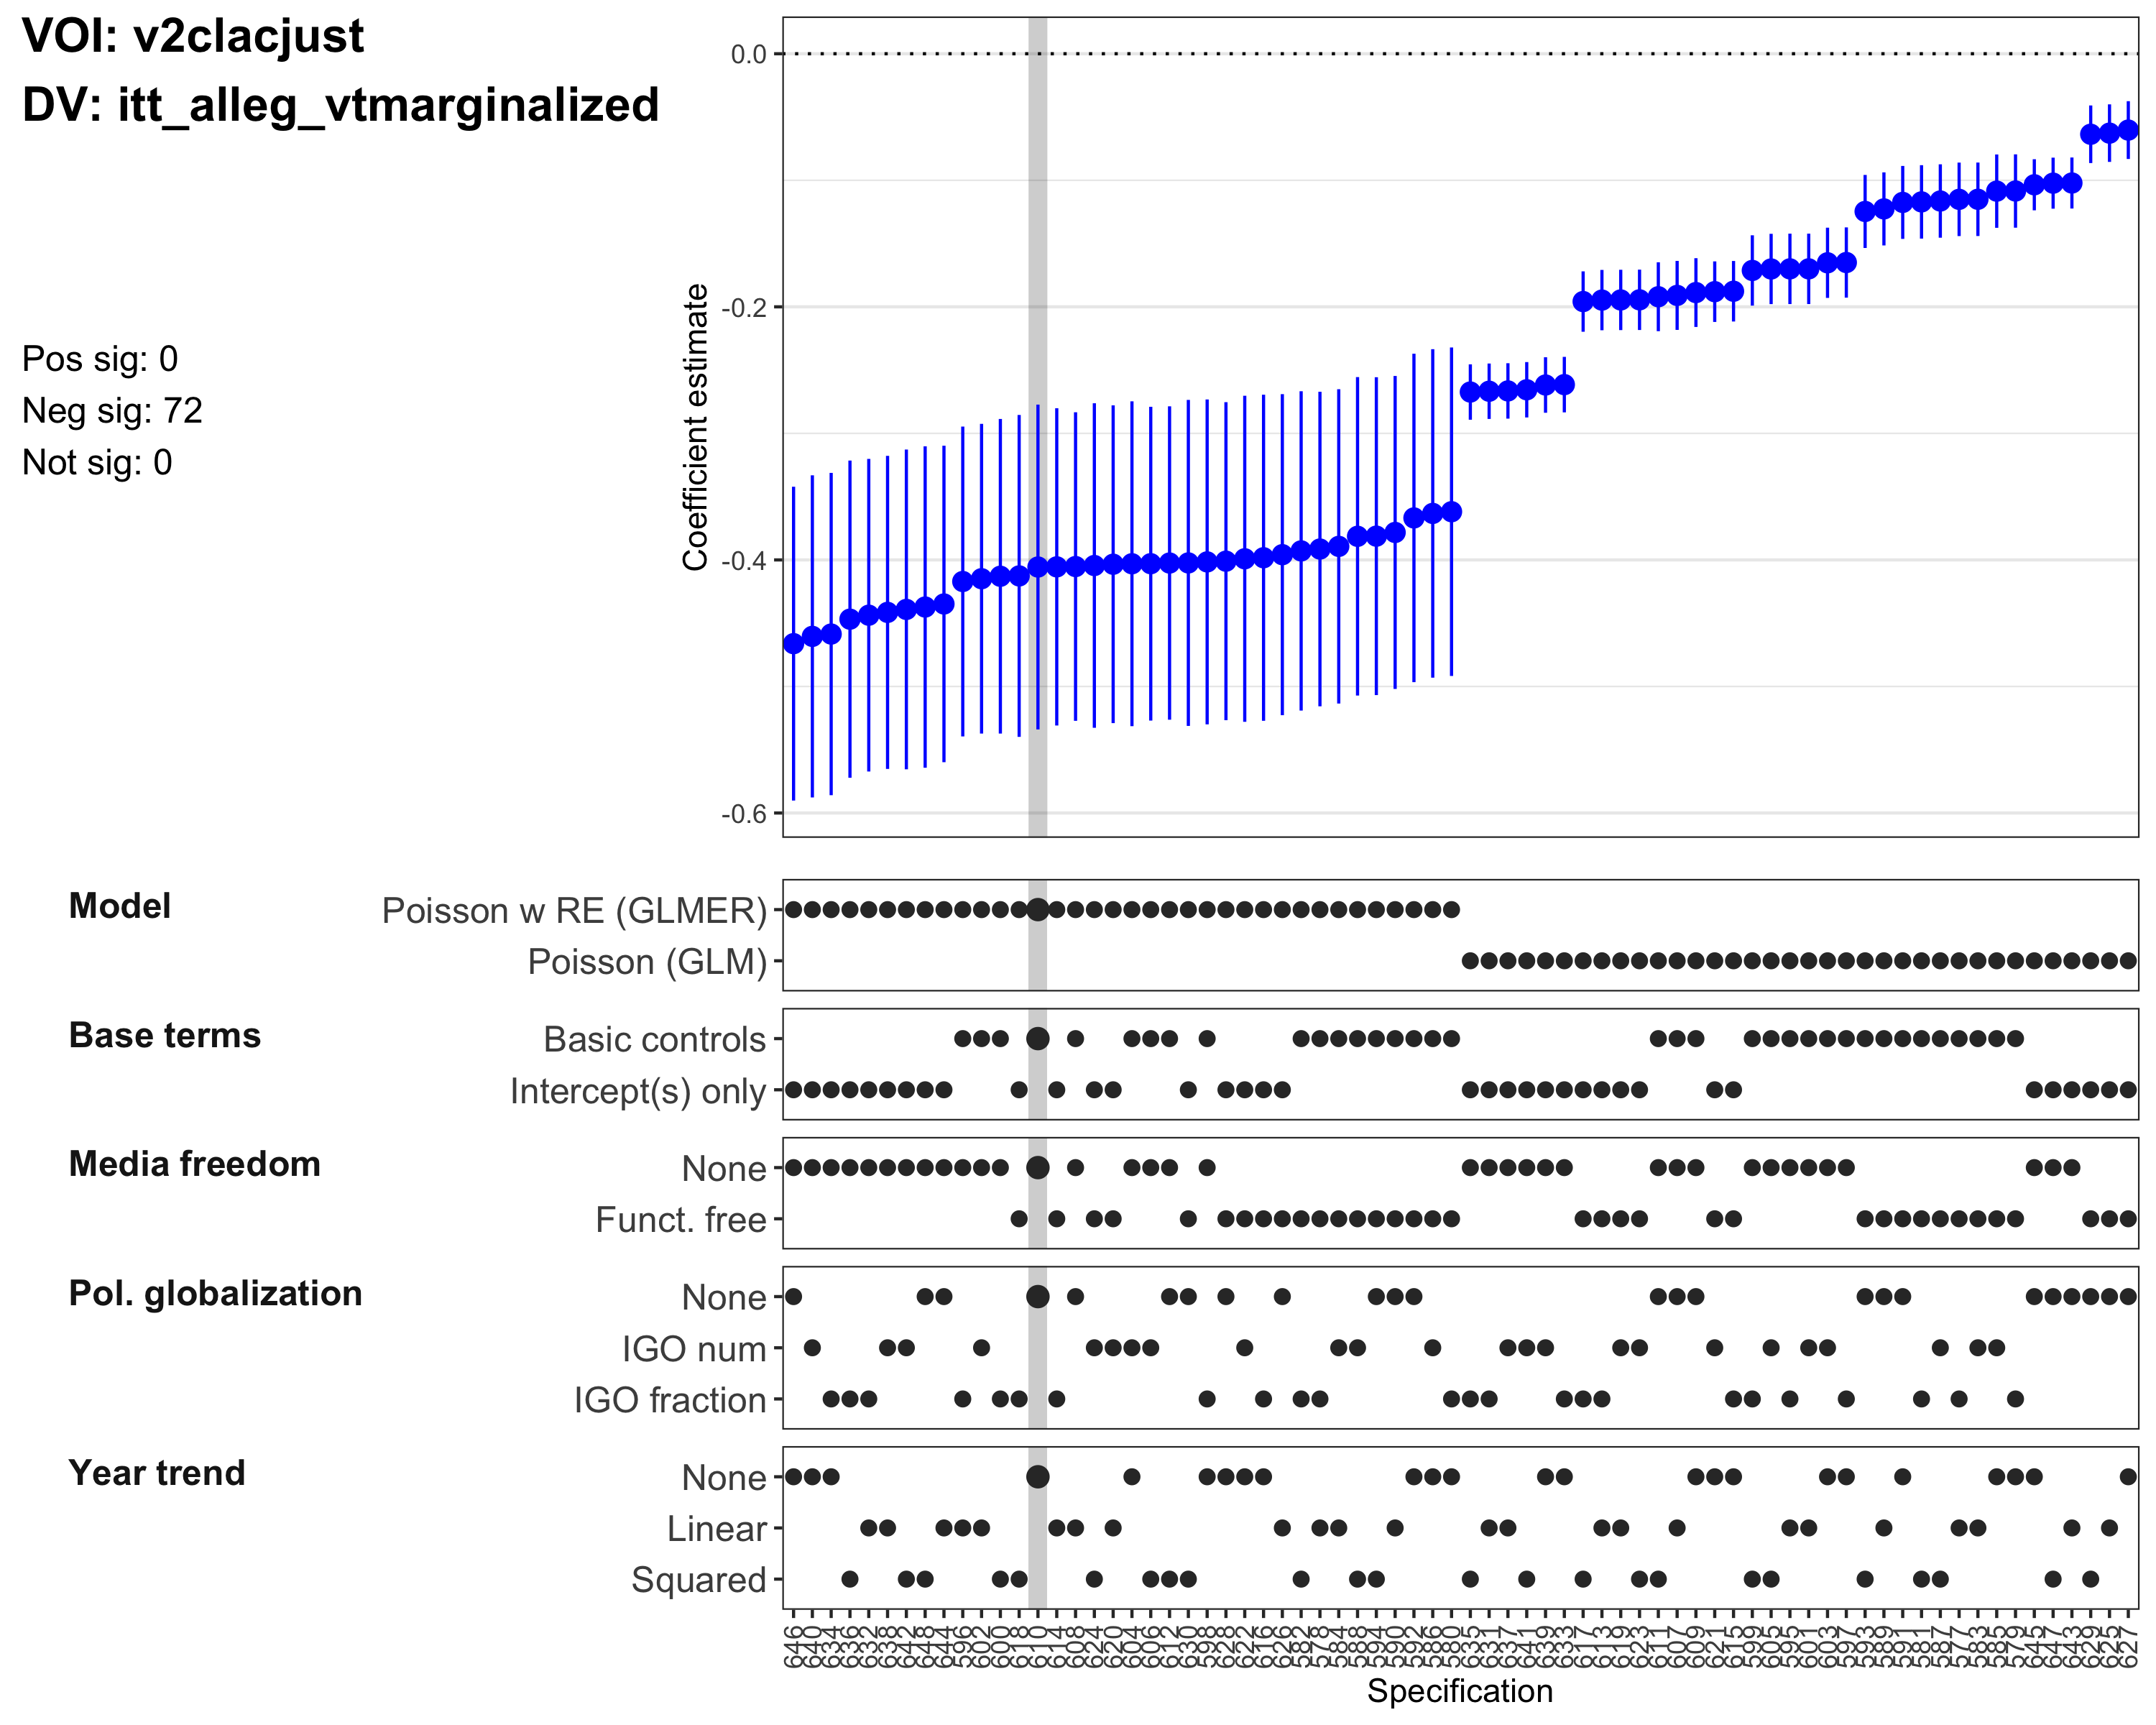
\includegraphics[height=4in]{../output/figures-robustness/specplot-v2clacjust-itt_alleg_vtmarginalized.png}

\hypertarget{voi-v2clsocgrp}{%
\subsection{VOI: v2clsocgrp}\label{voi-v2clsocgrp}}

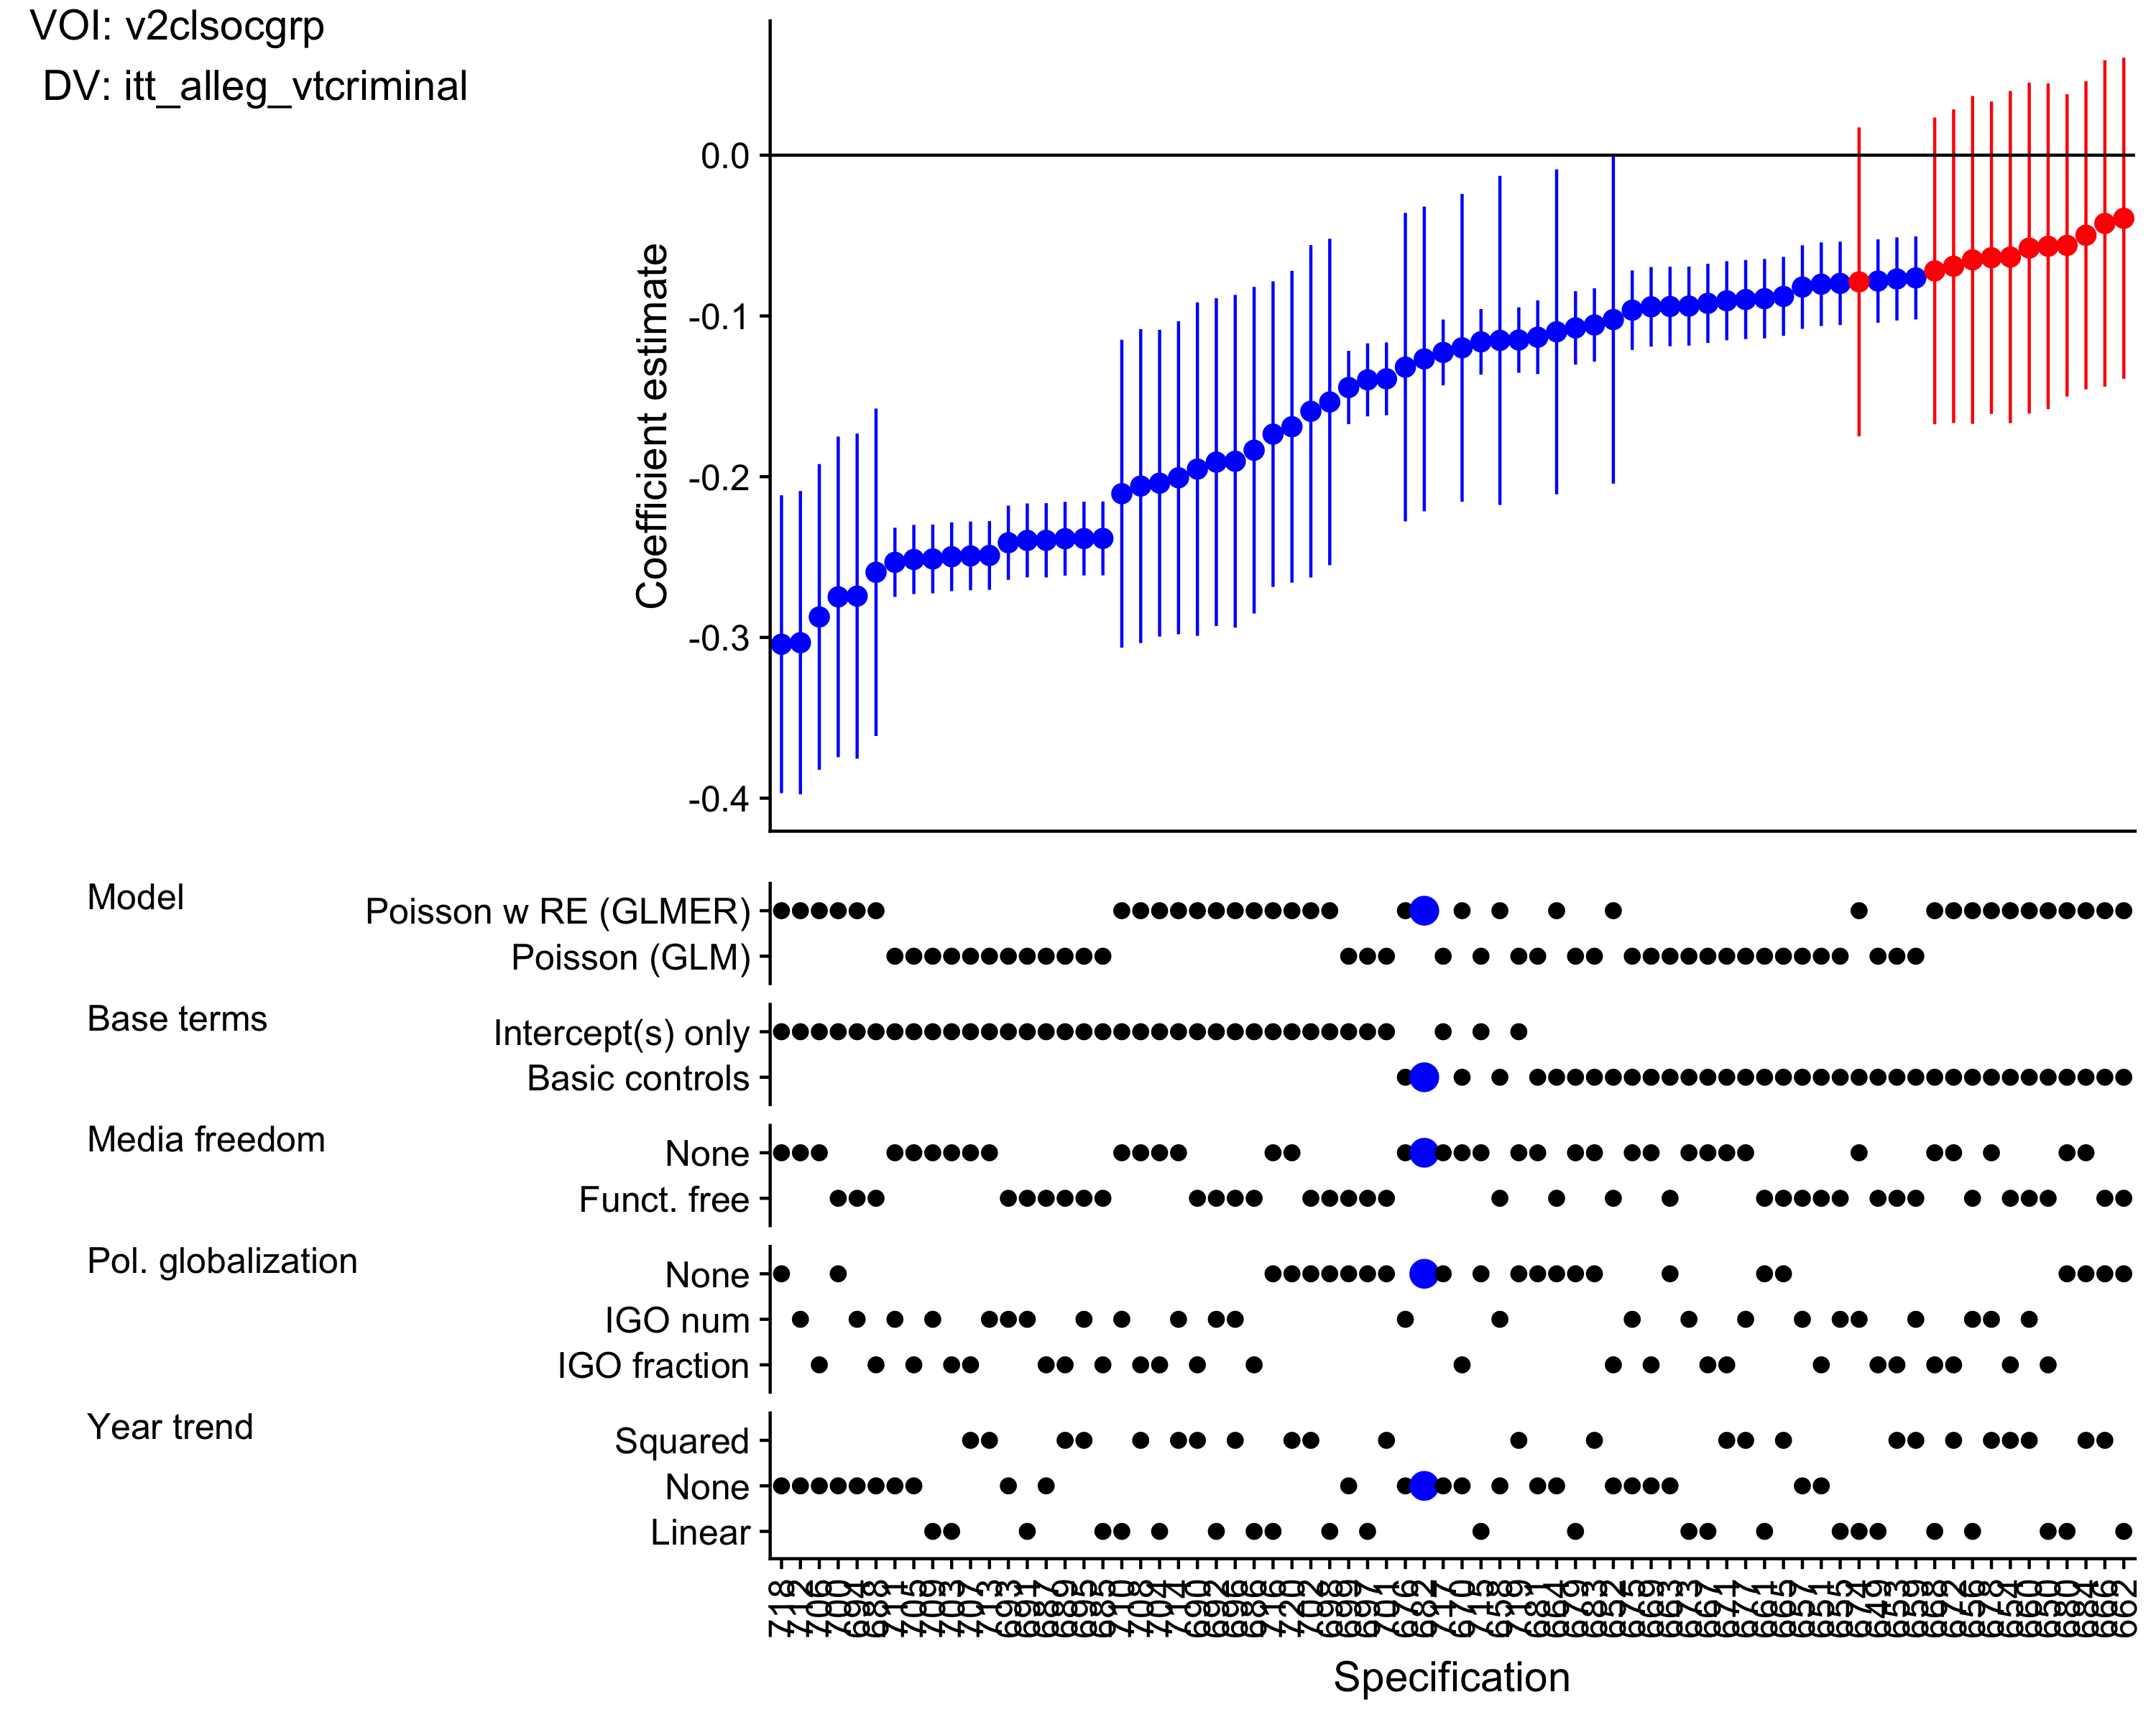
\includegraphics[height=4in]{../output/figures-robustness/specplot-v2clsocgrp-itt_alleg_vtcriminal.png}

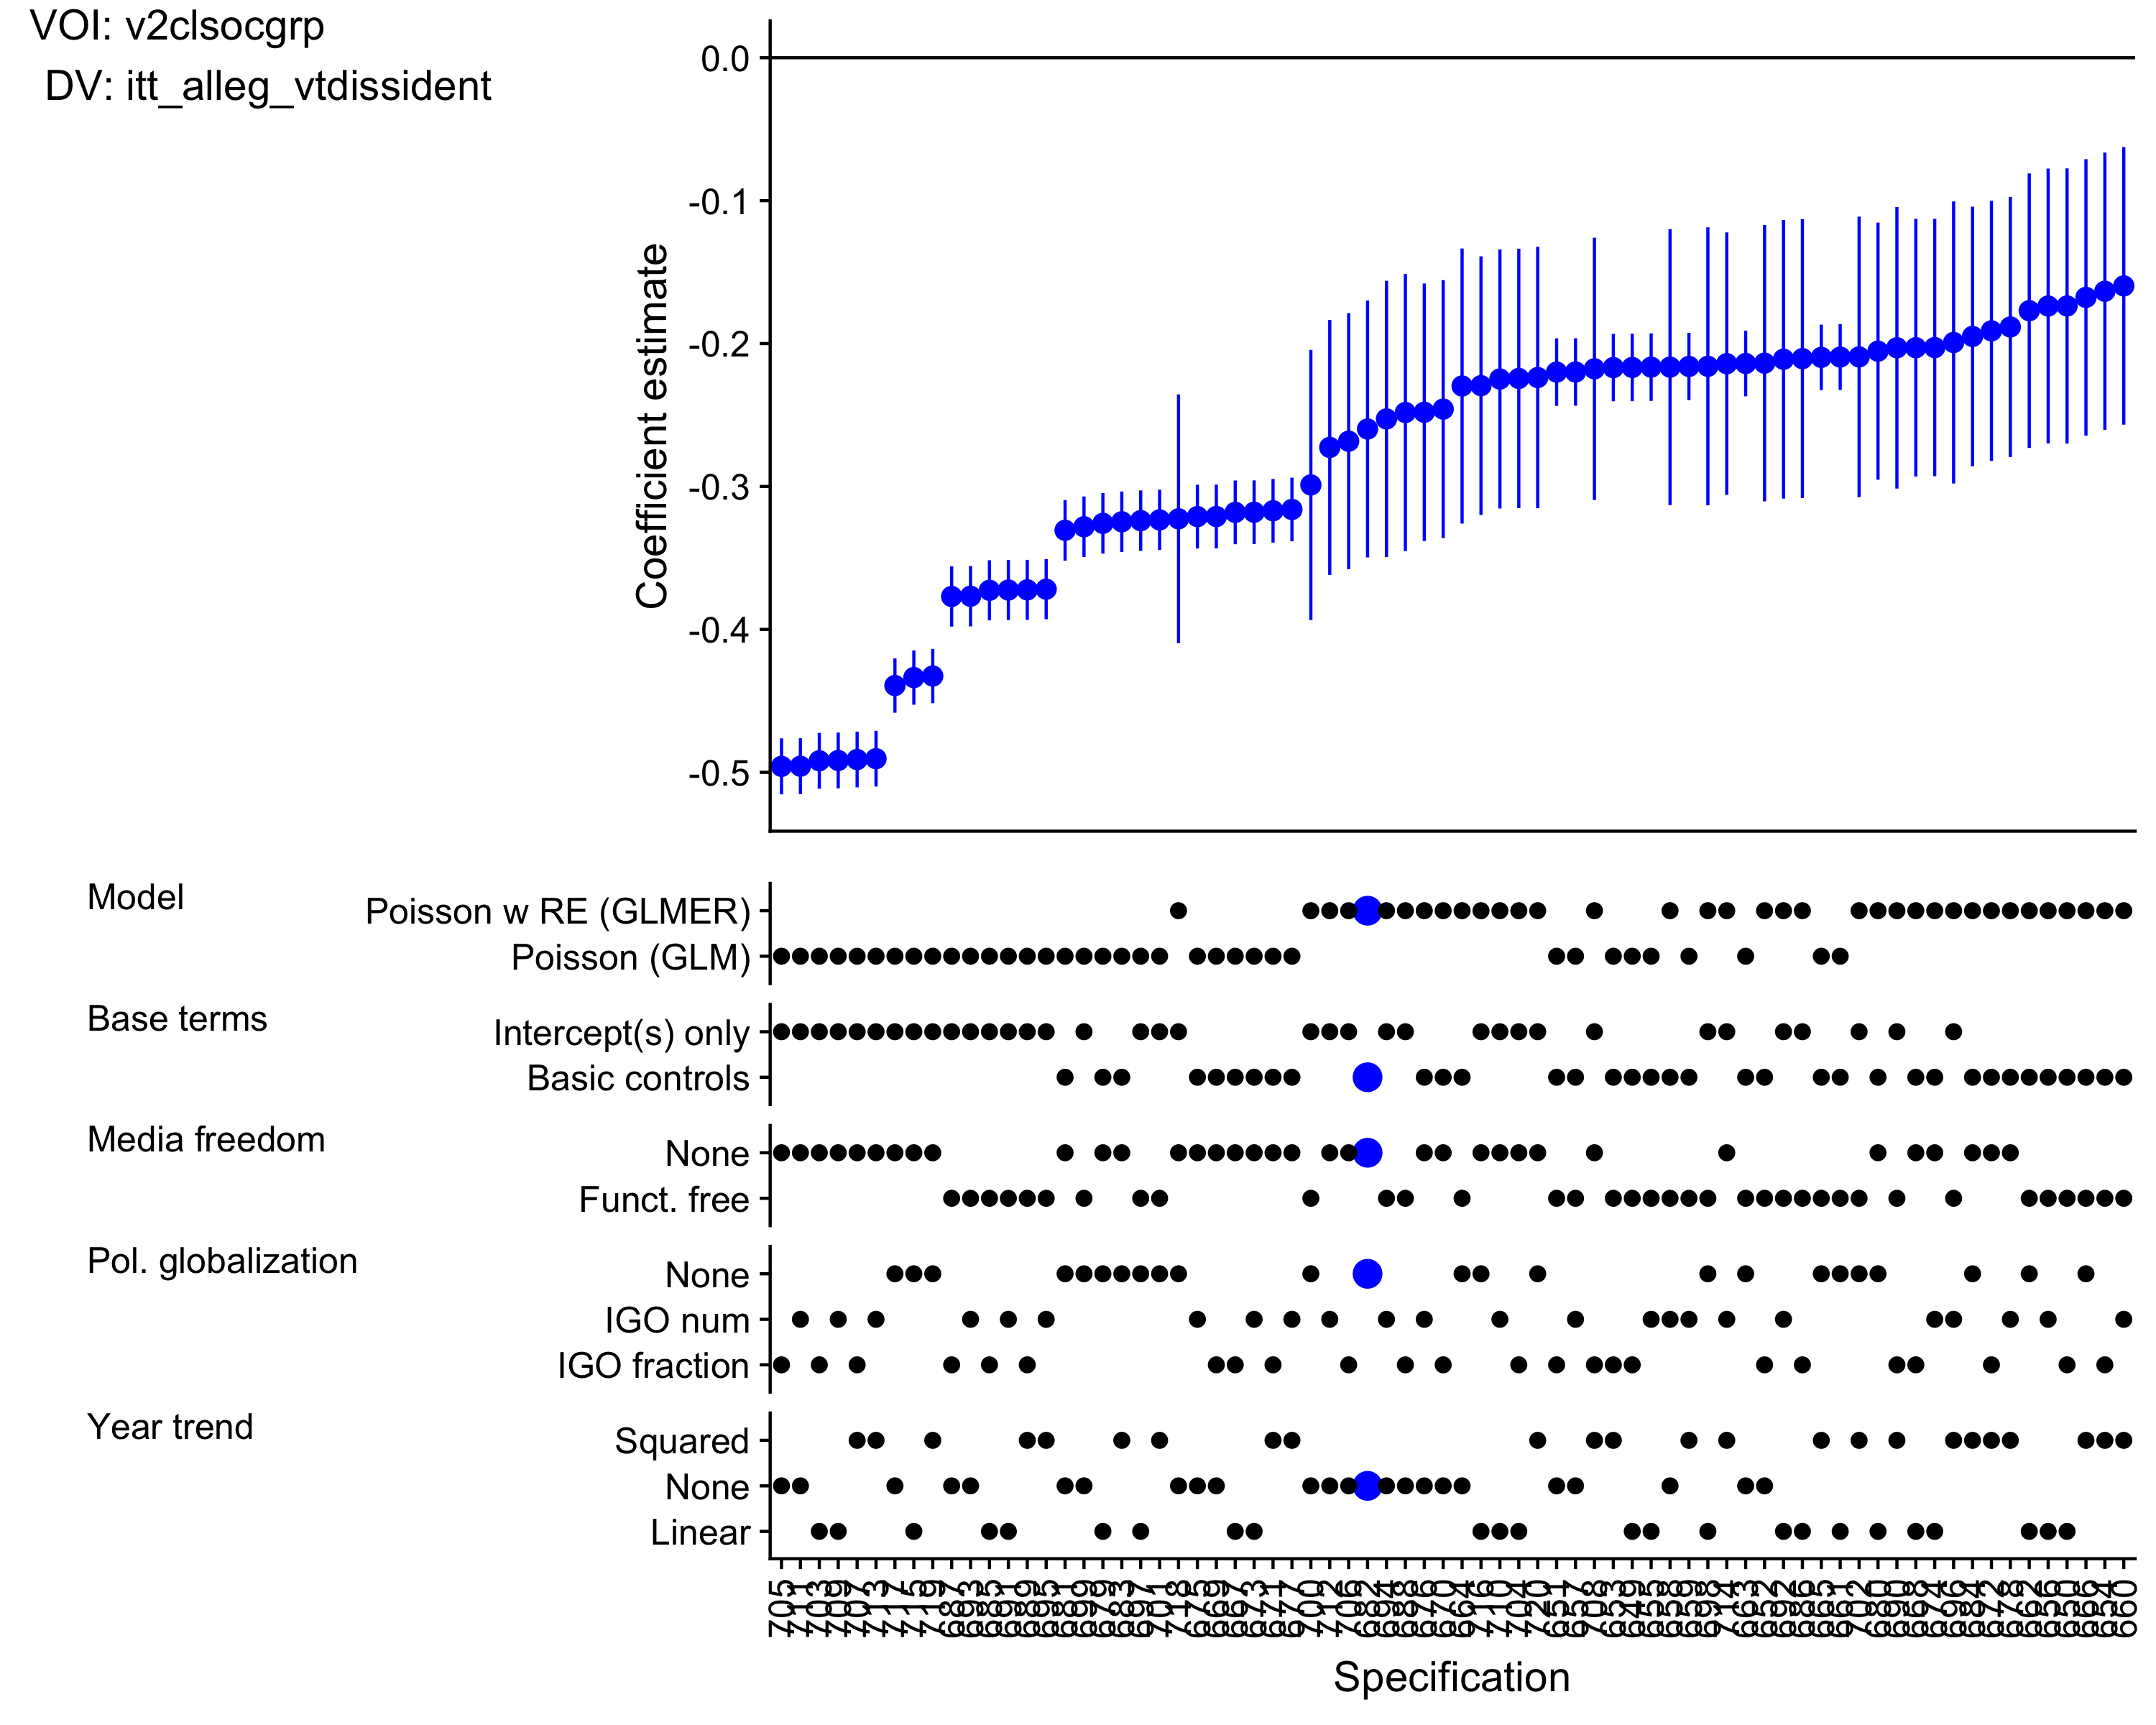
\includegraphics[height=4in]{../output/figures-robustness/specplot-v2clsocgrp-itt_alleg_vtdissident.png}

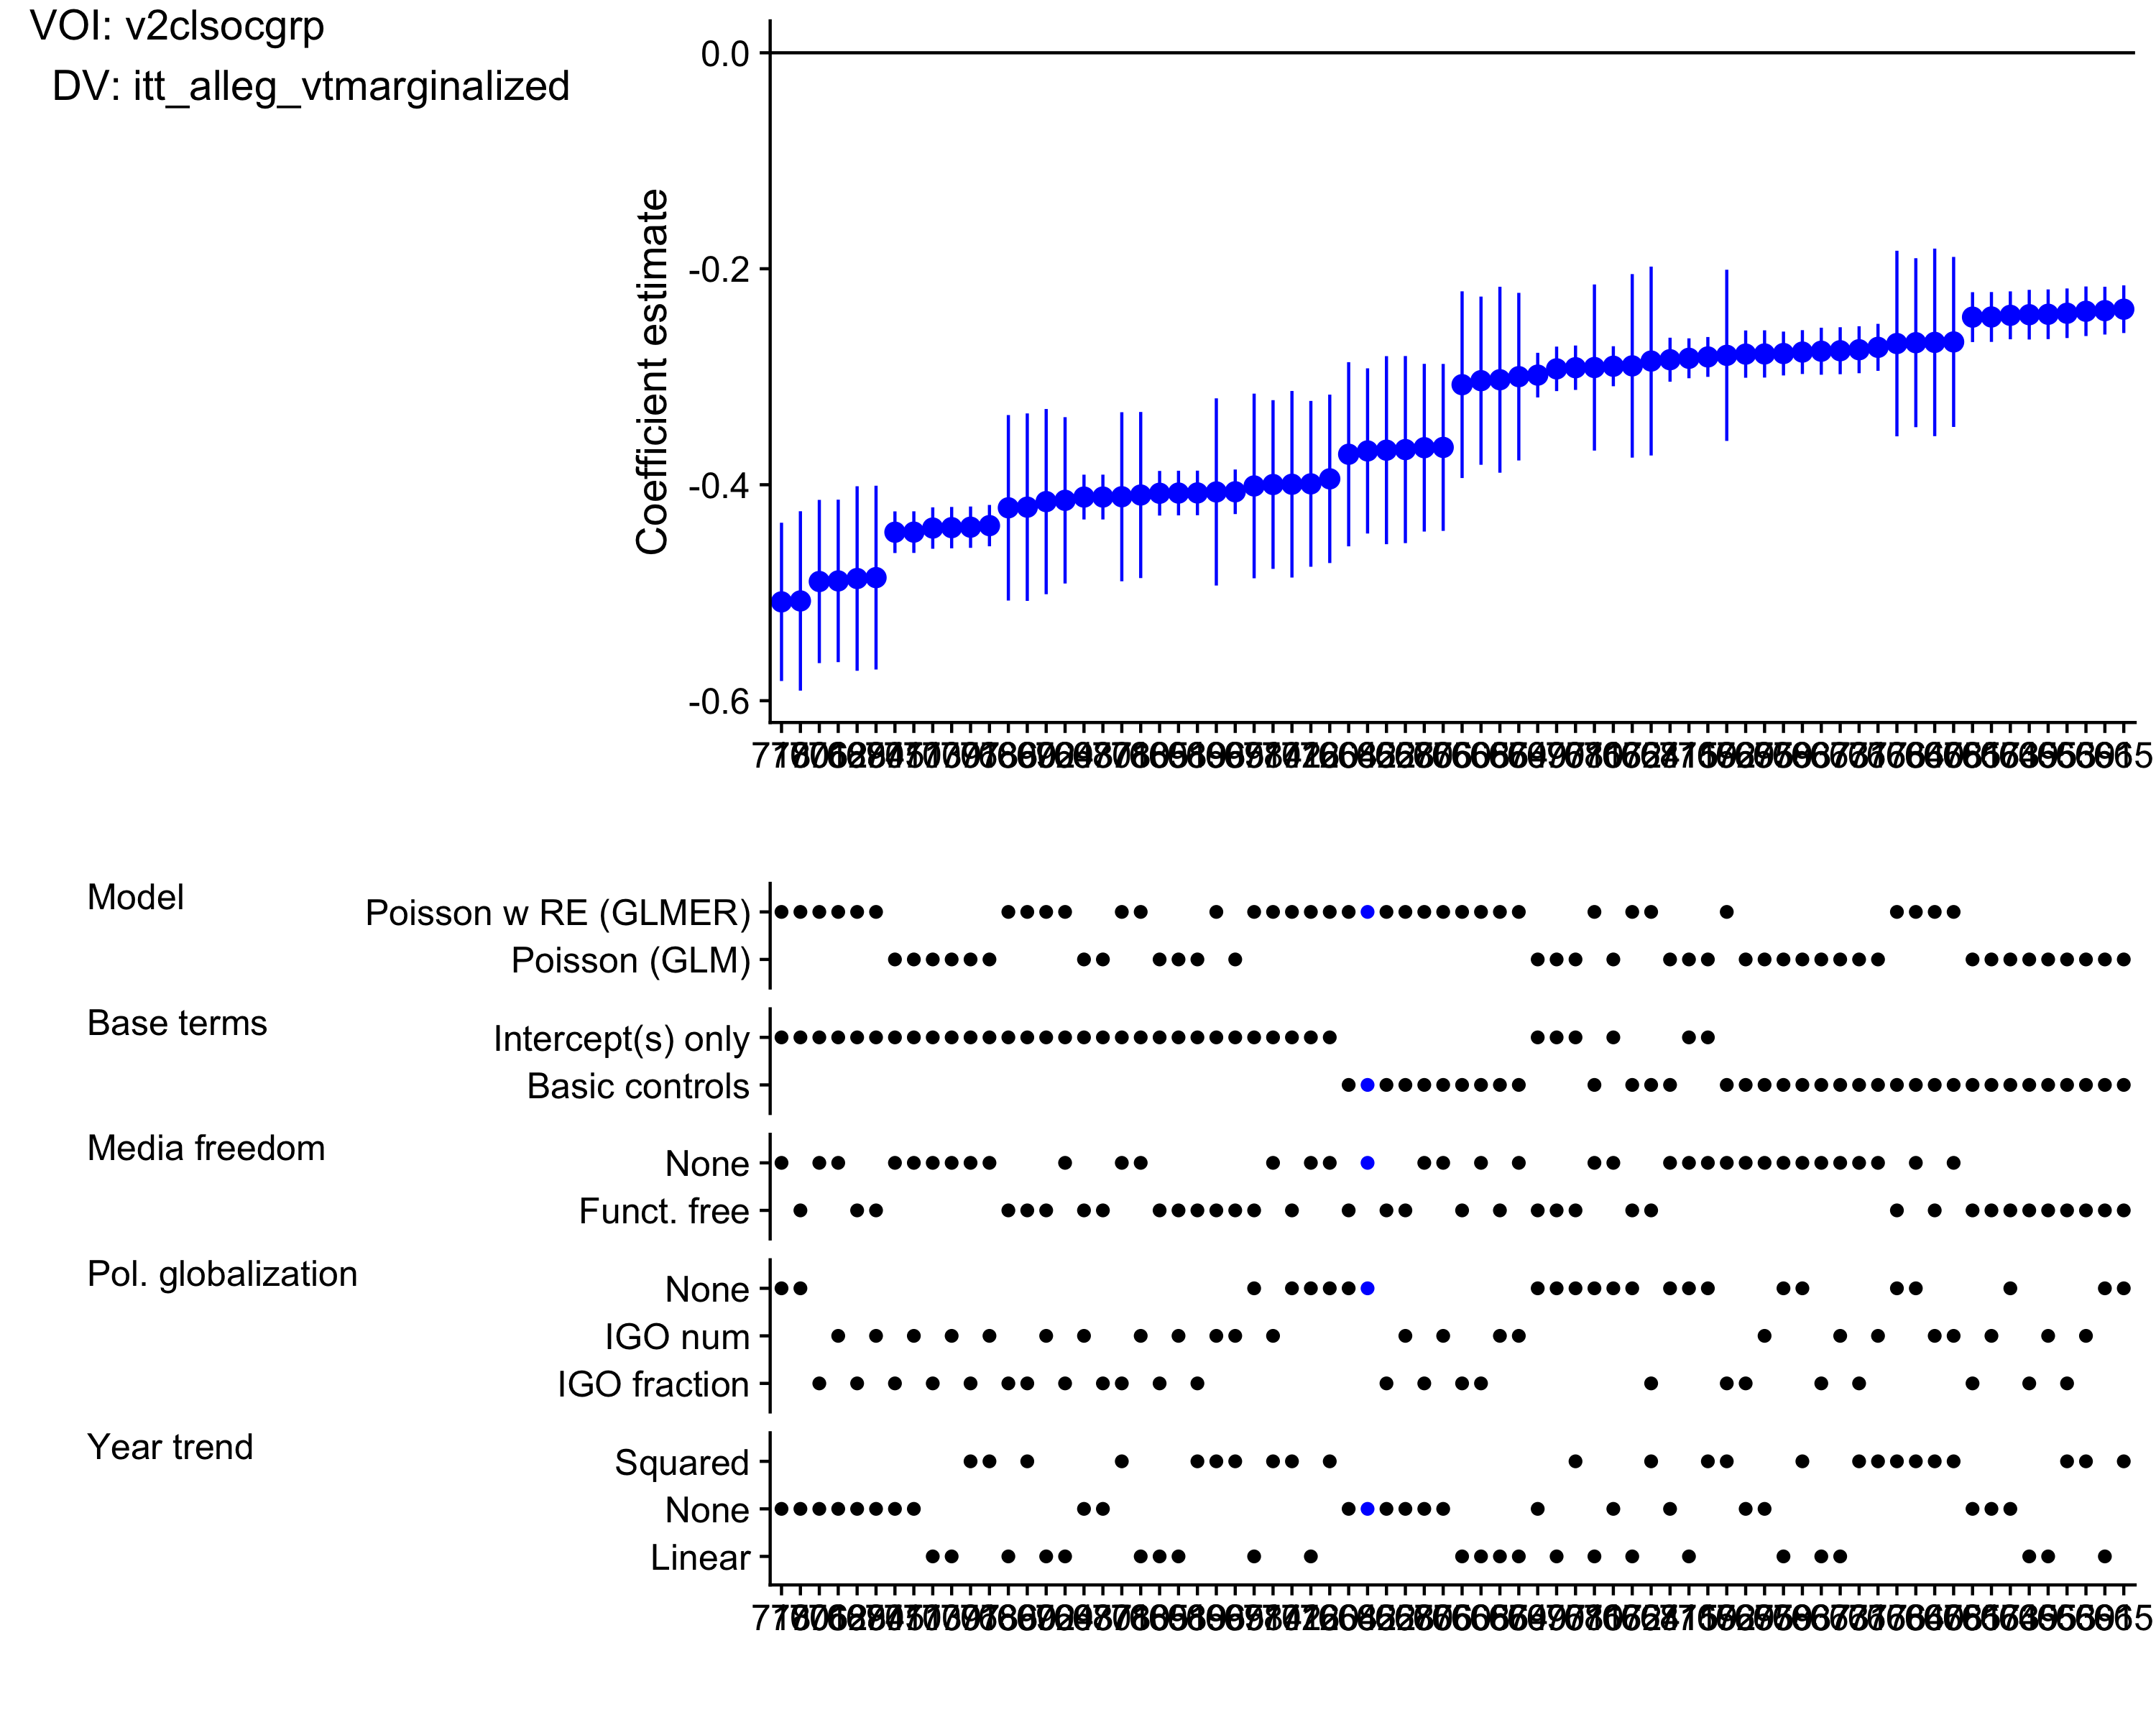
\includegraphics[height=4in]{../output/figures-robustness/specplot-v2clsocgrp-itt_alleg_vtmarginalized.png}

\hypertarget{voi-v2pepwrses}{%
\subsection{VOI: v2pepwrses}\label{voi-v2pepwrses}}

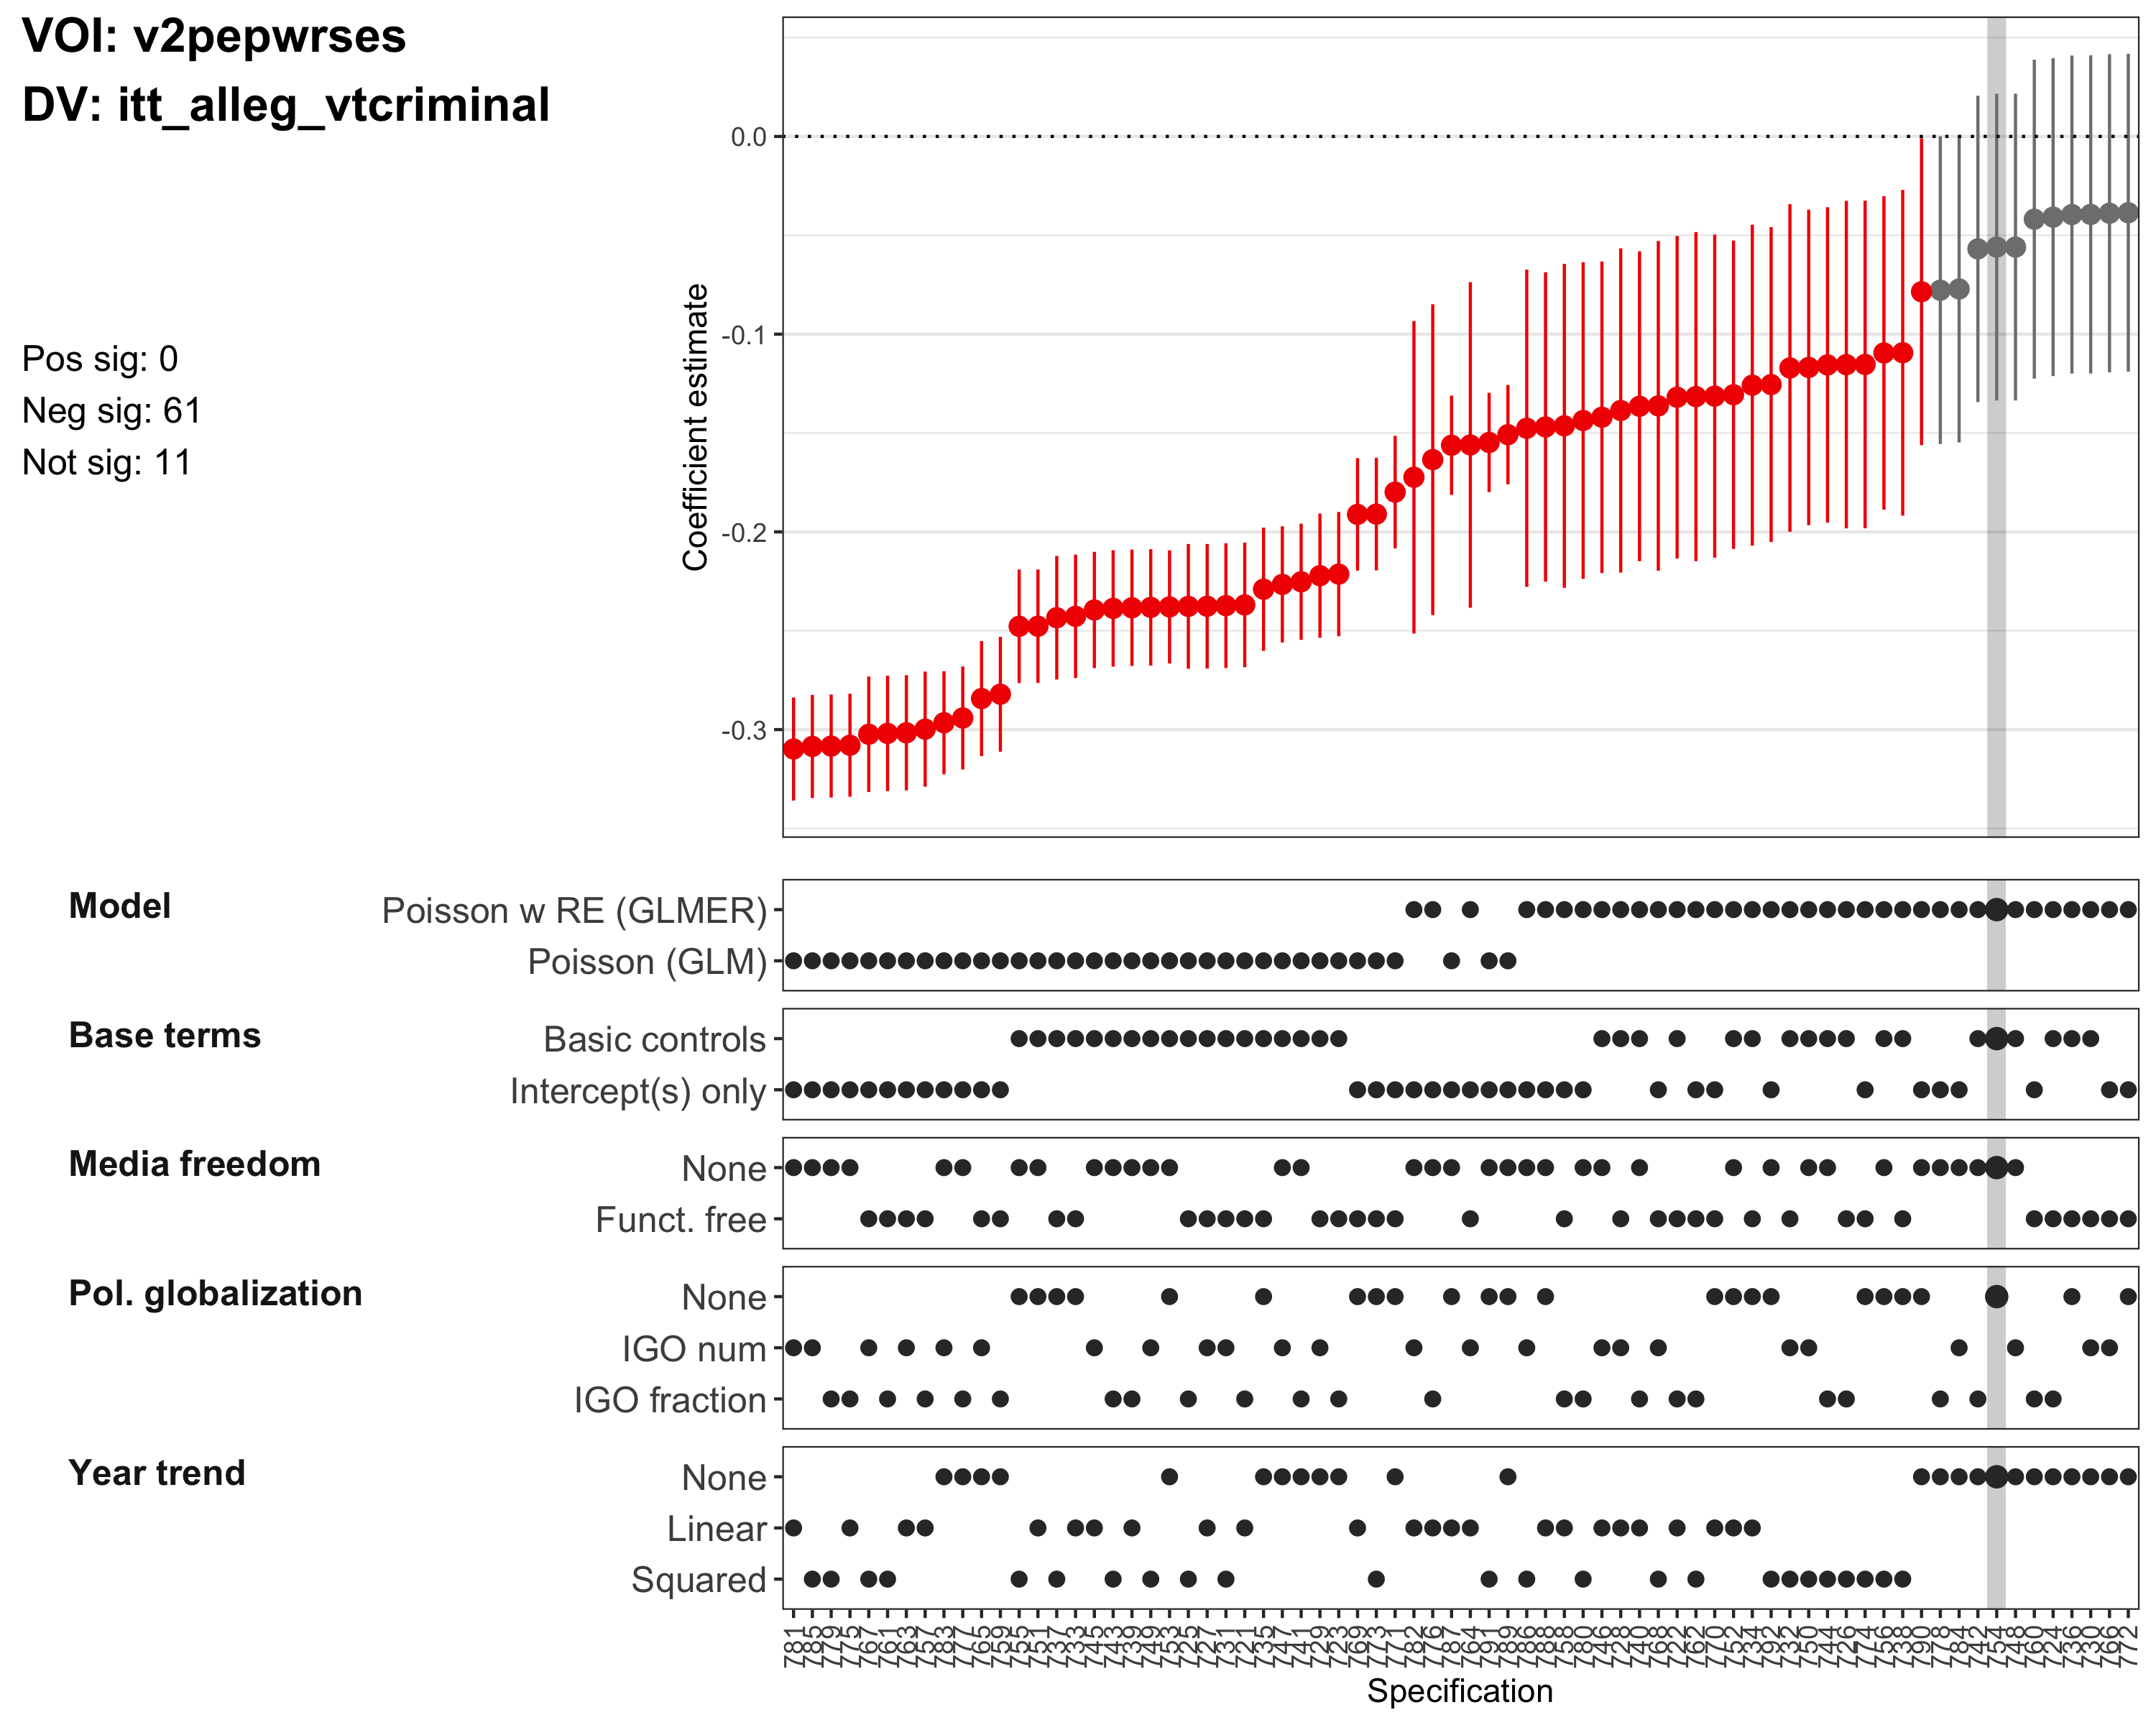
\includegraphics[height=4in]{../output/figures-robustness/specplot-v2pepwrses-itt_alleg_vtcriminal.png}

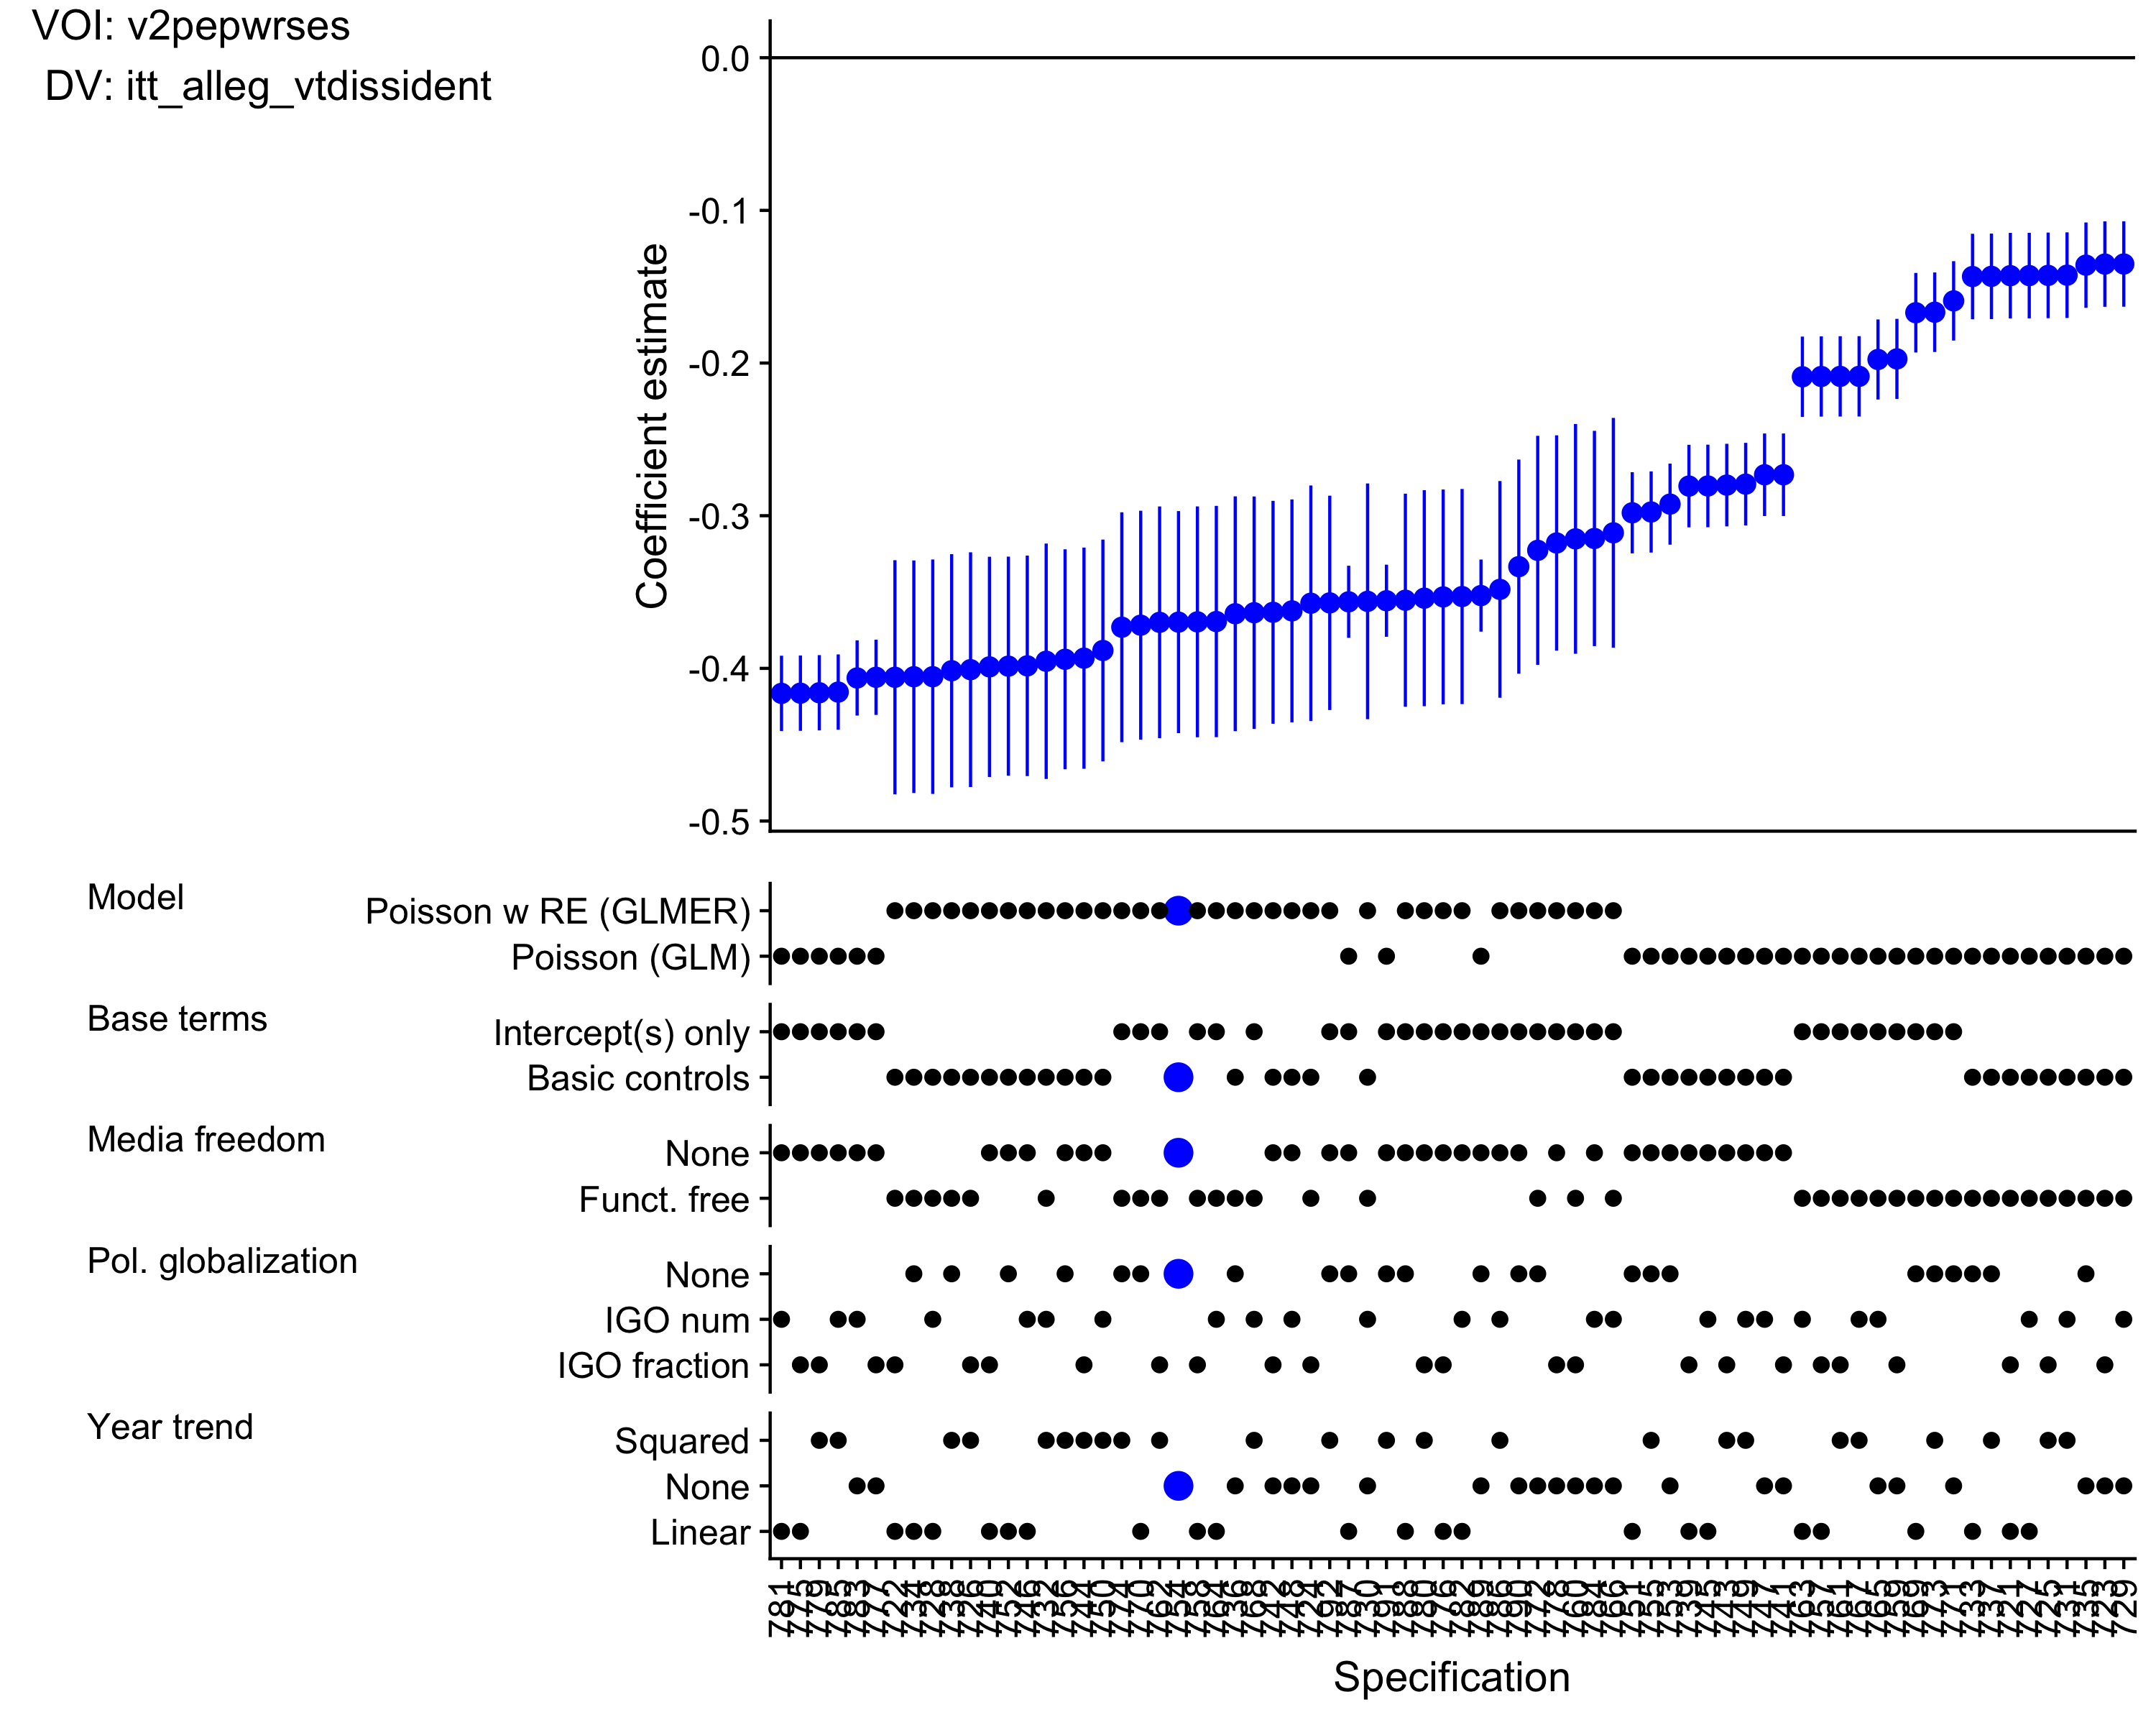
\includegraphics[height=4in]{../output/figures-robustness/specplot-v2pepwrses-itt_alleg_vtdissident.png}

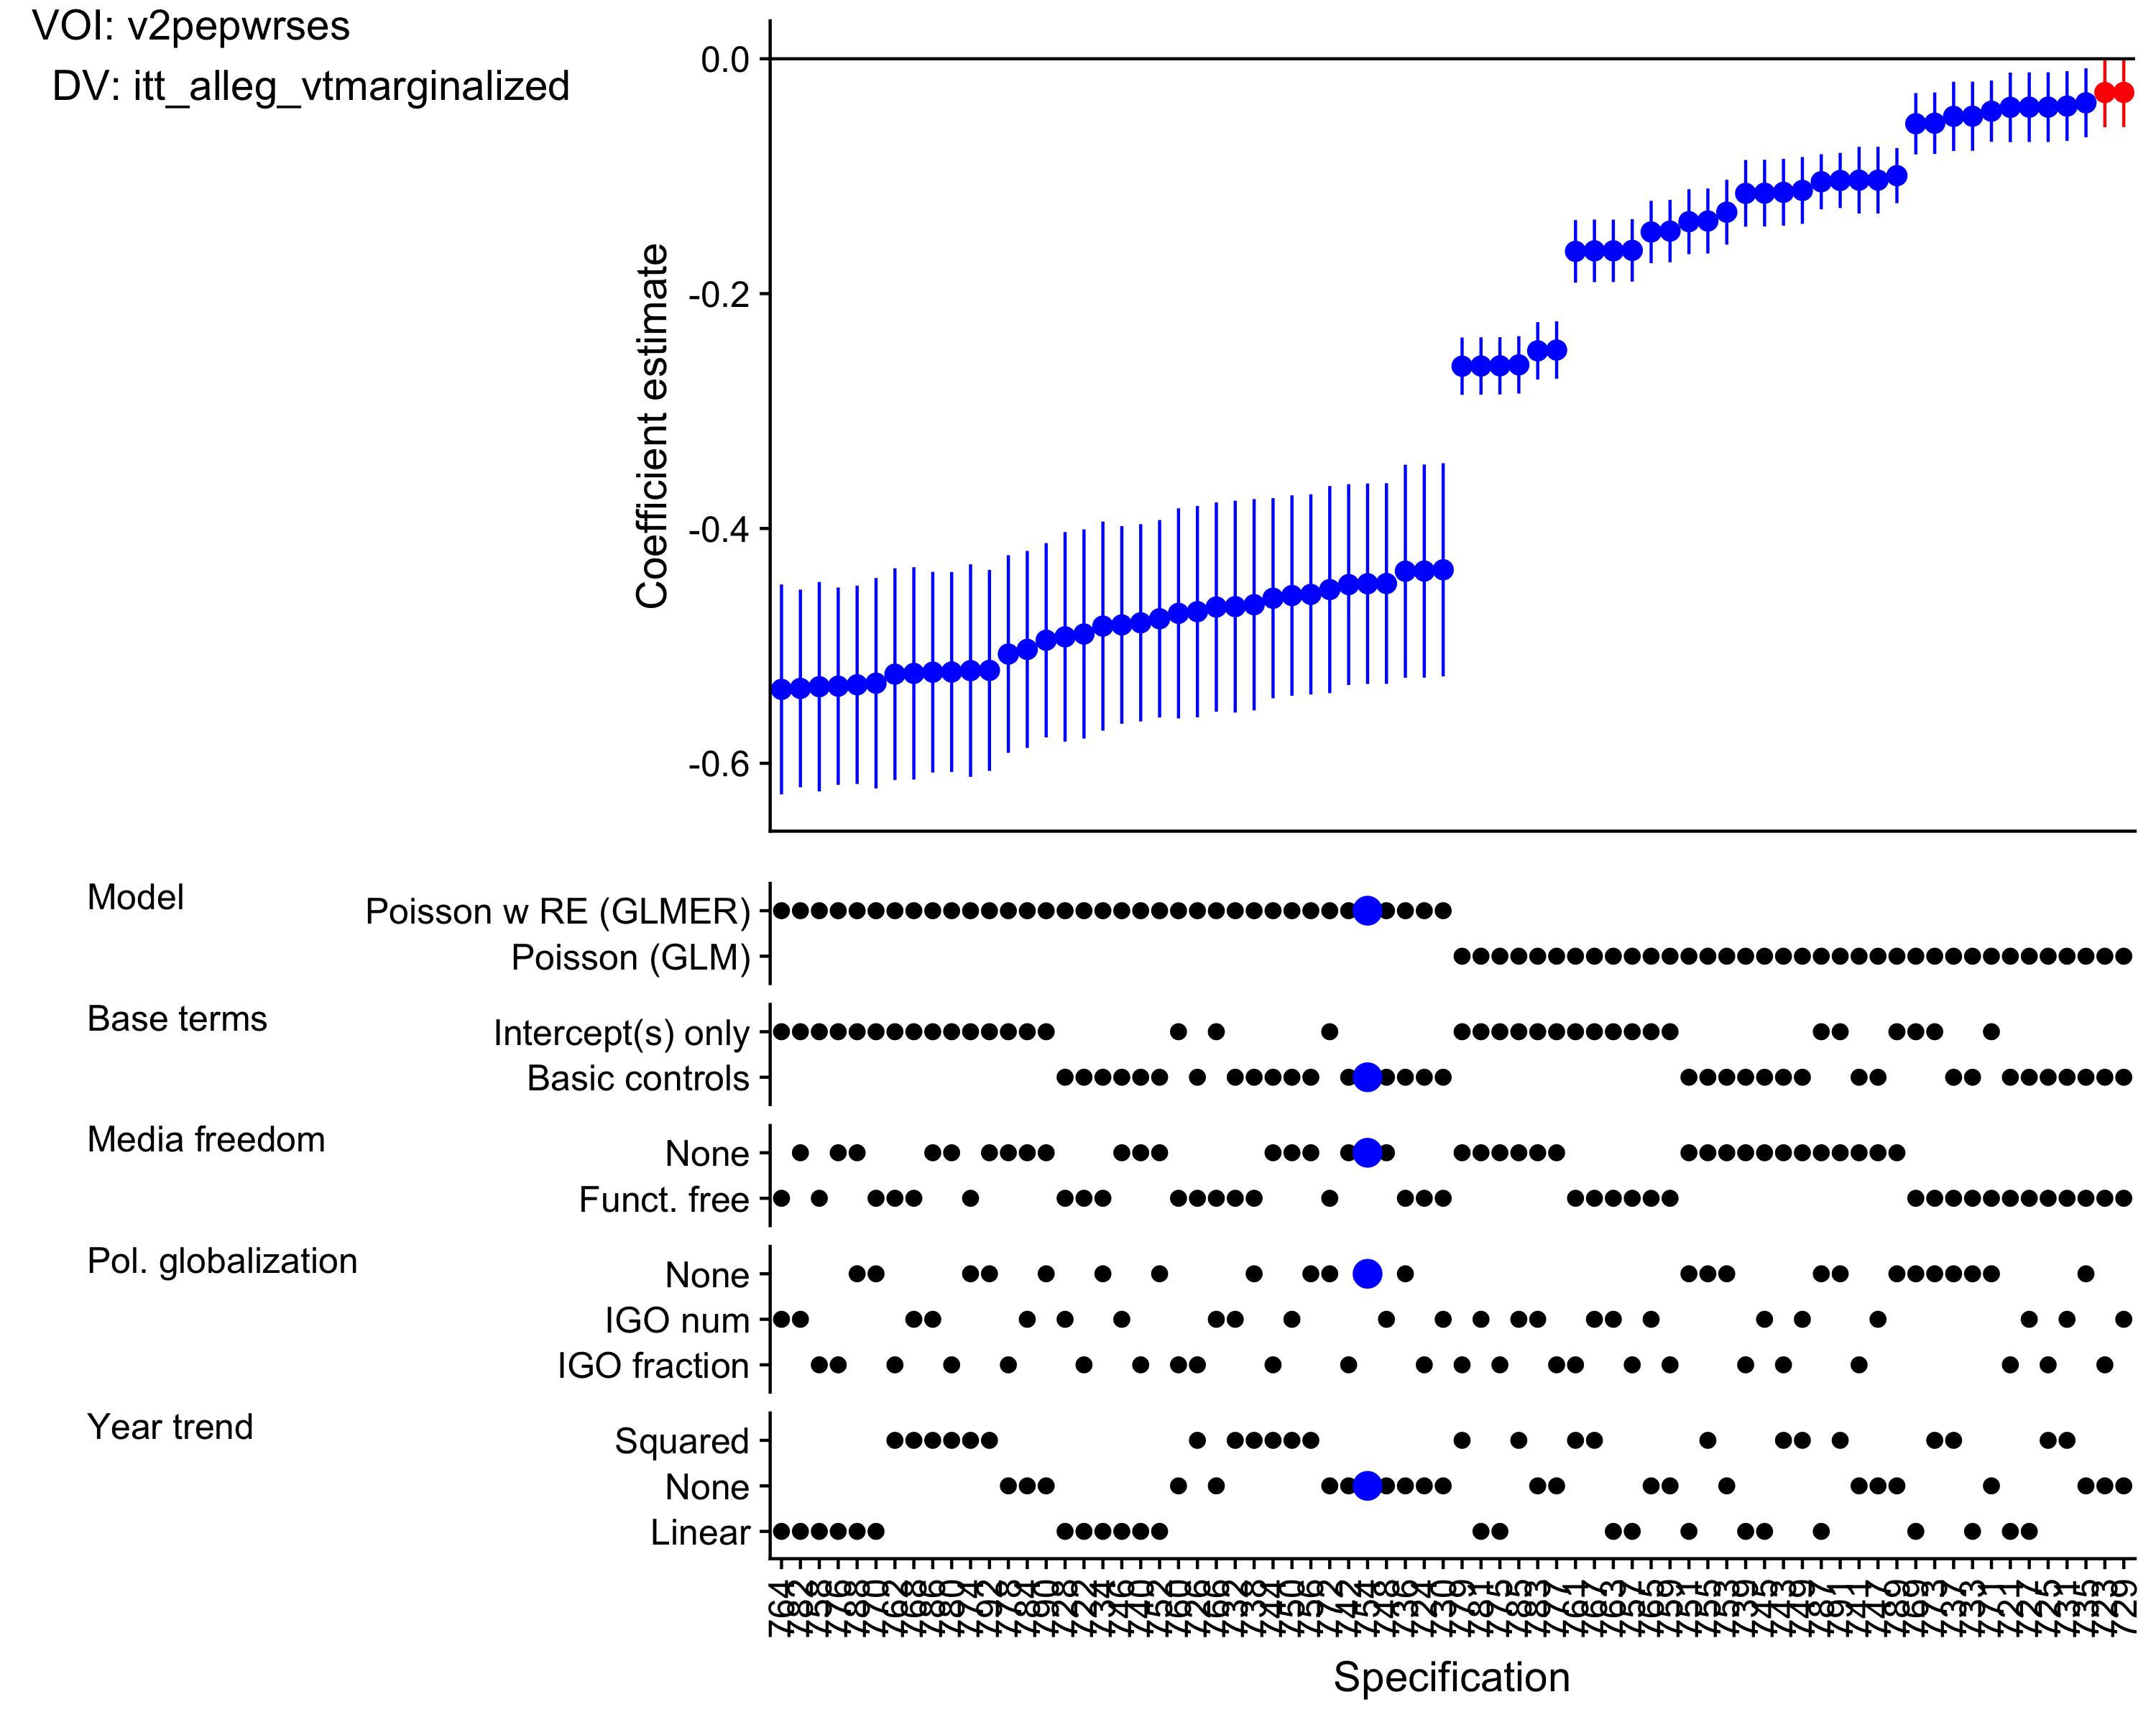
\includegraphics[height=4in]{../output/figures-robustness/specplot-v2pepwrses-itt_alleg_vtmarginalized.png}

\hypertarget{voi-v2pepwrsoc}{%
\subsection{VOI: v2pepwrsoc}\label{voi-v2pepwrsoc}}

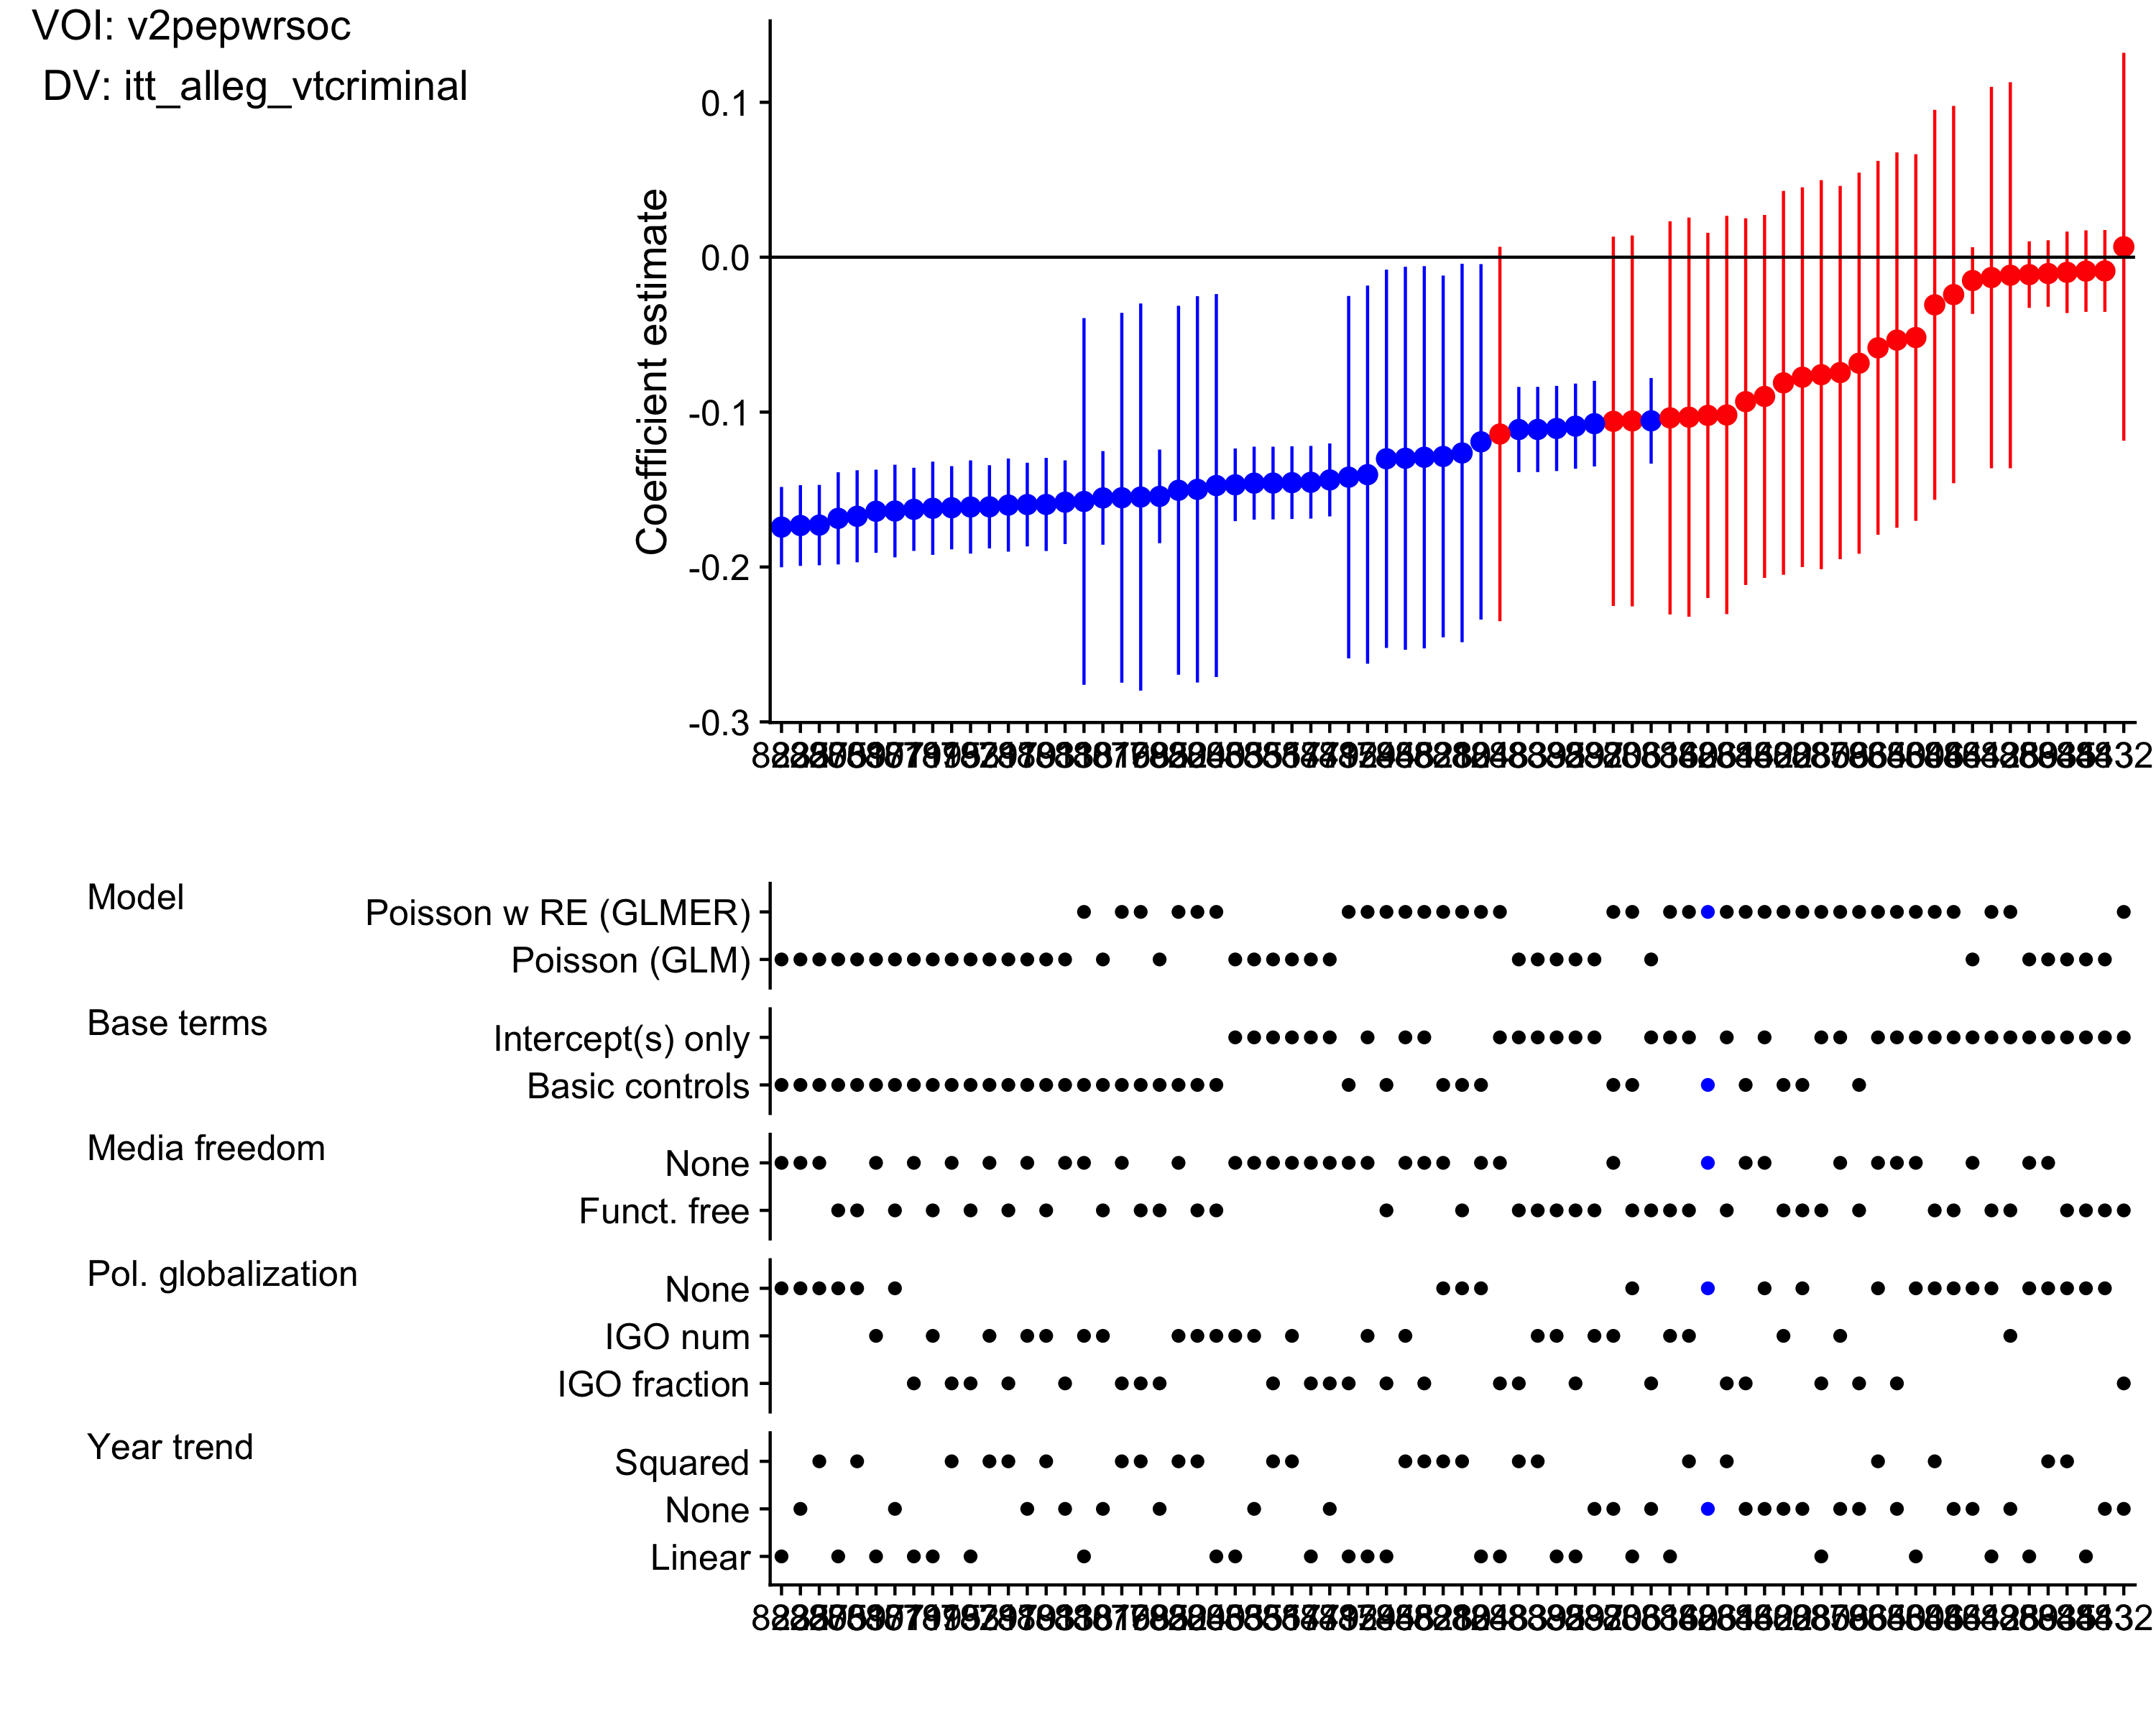
\includegraphics[height=4in]{../output/figures-robustness/specplot-v2pepwrsoc-itt_alleg_vtcriminal.png}

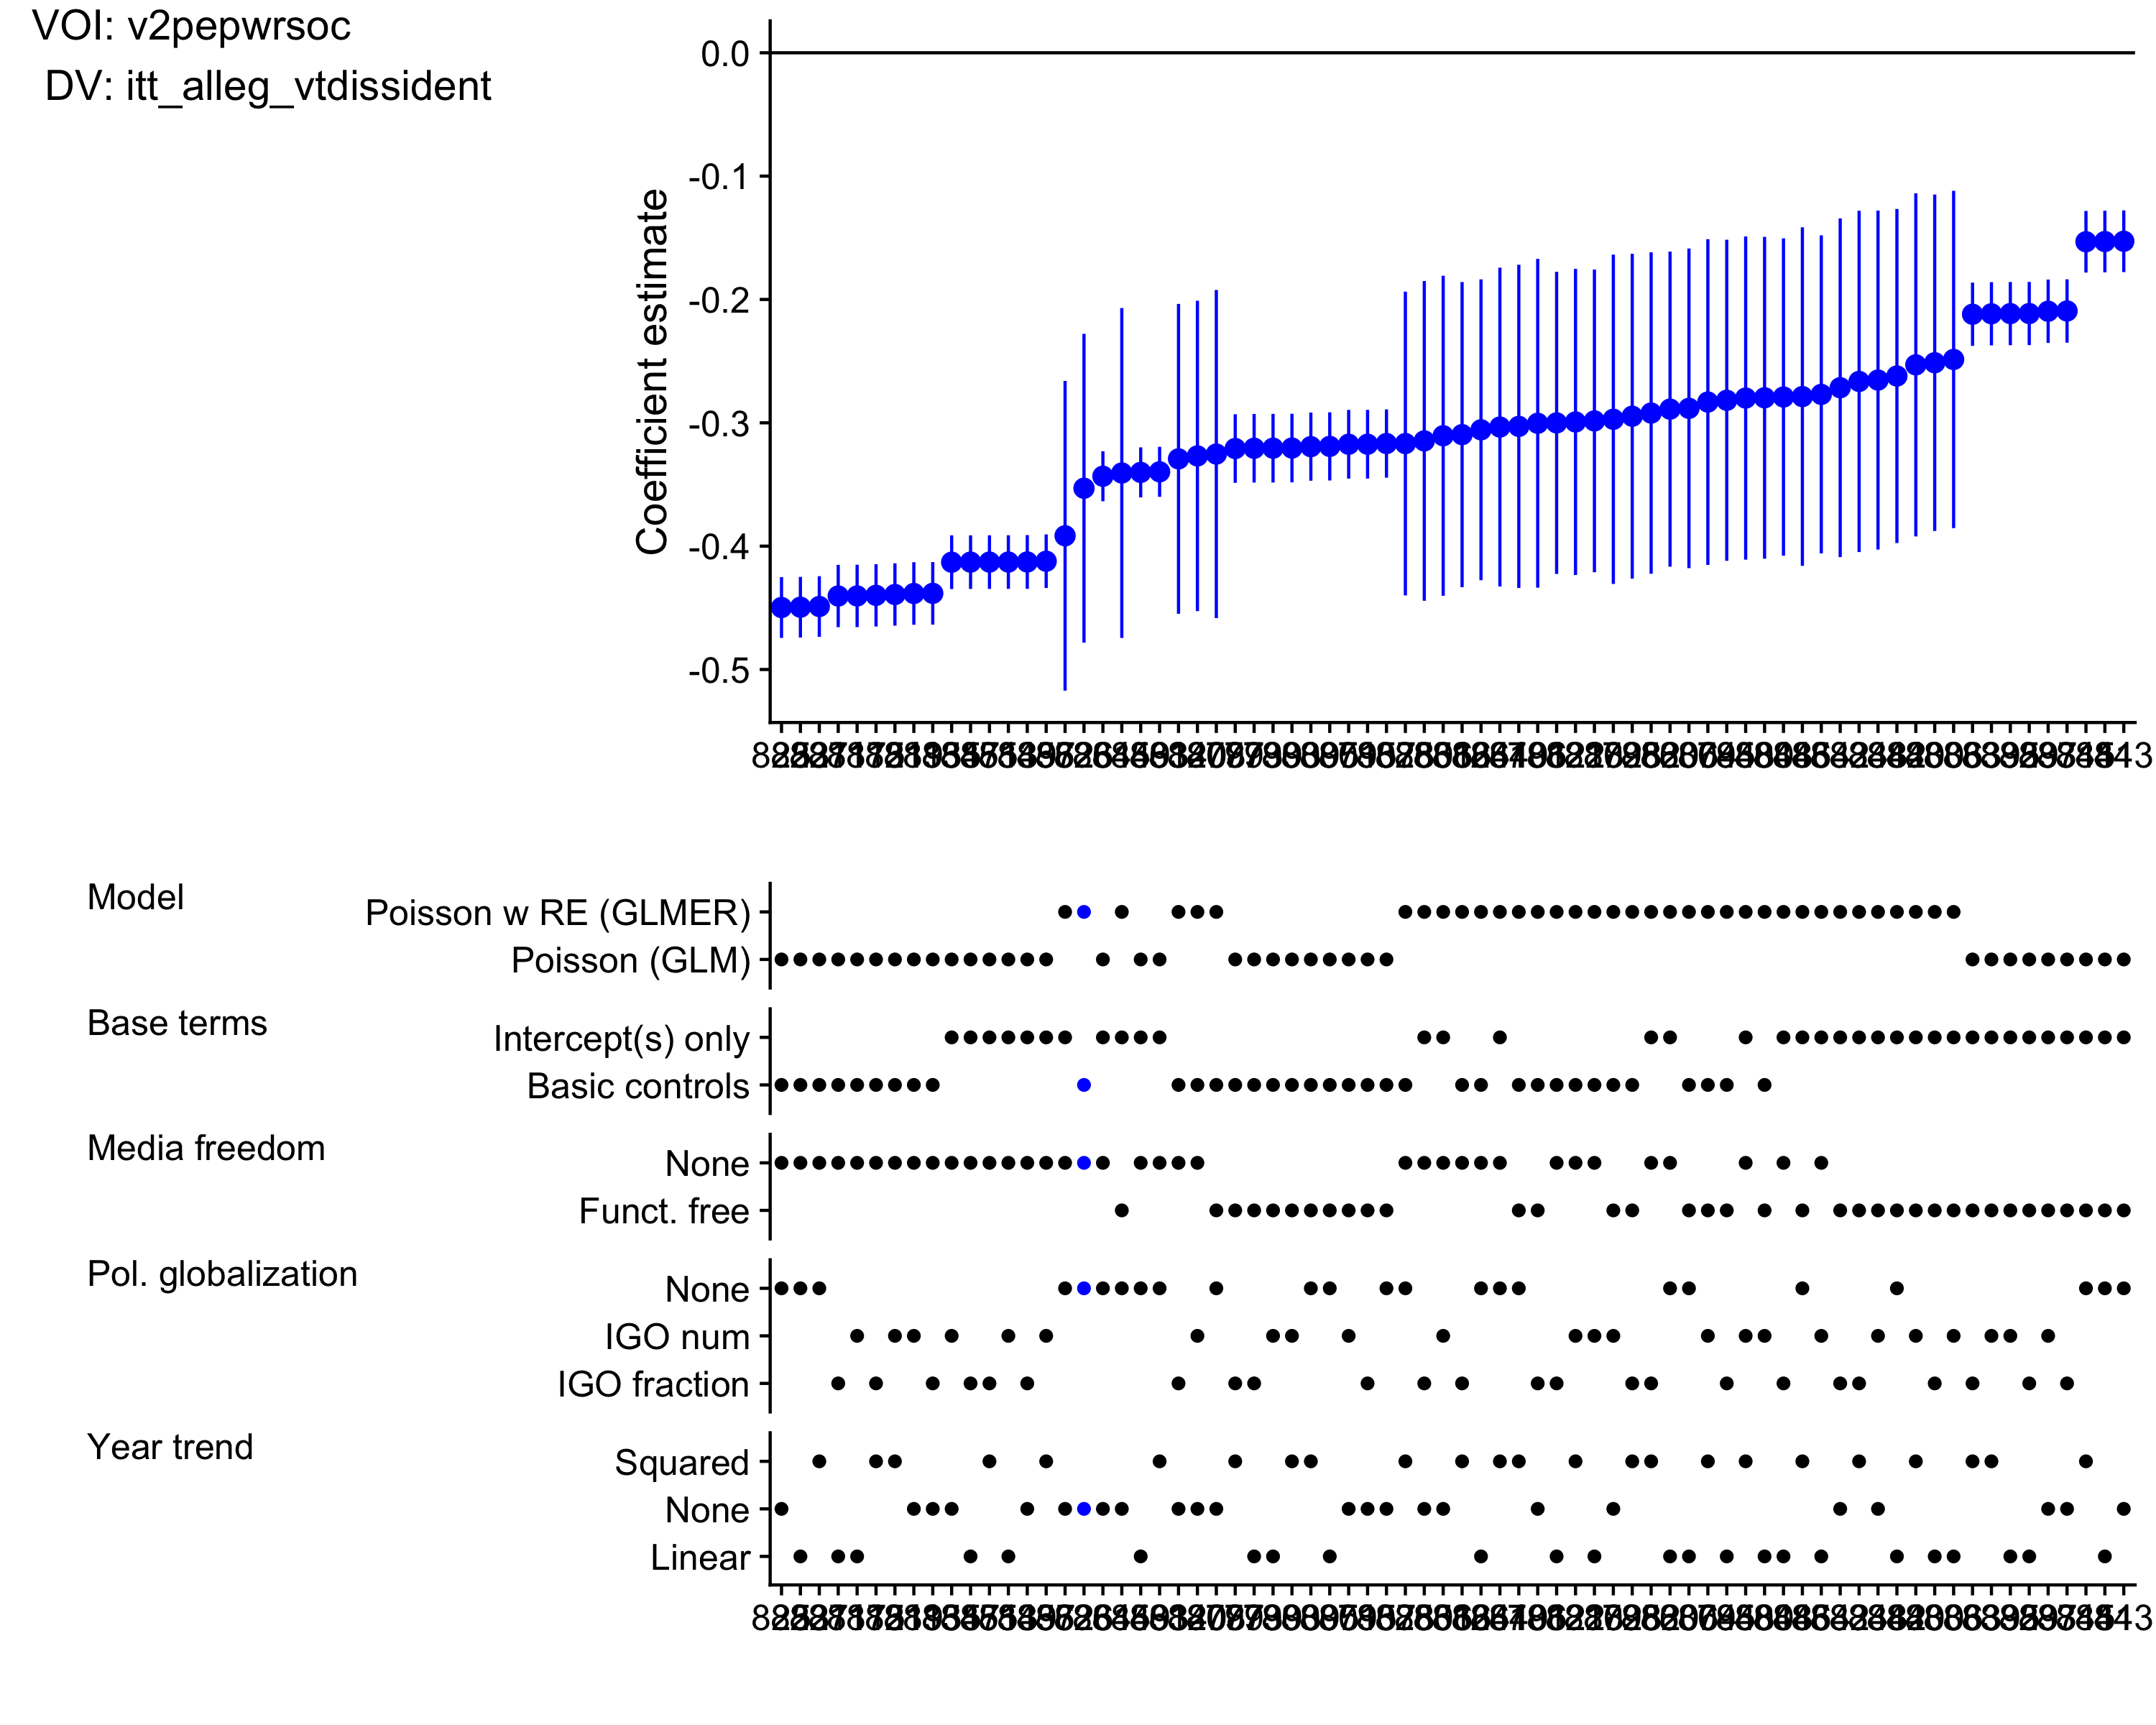
\includegraphics[height=4in]{../output/figures-robustness/specplot-v2pepwrsoc-itt_alleg_vtdissident.png}

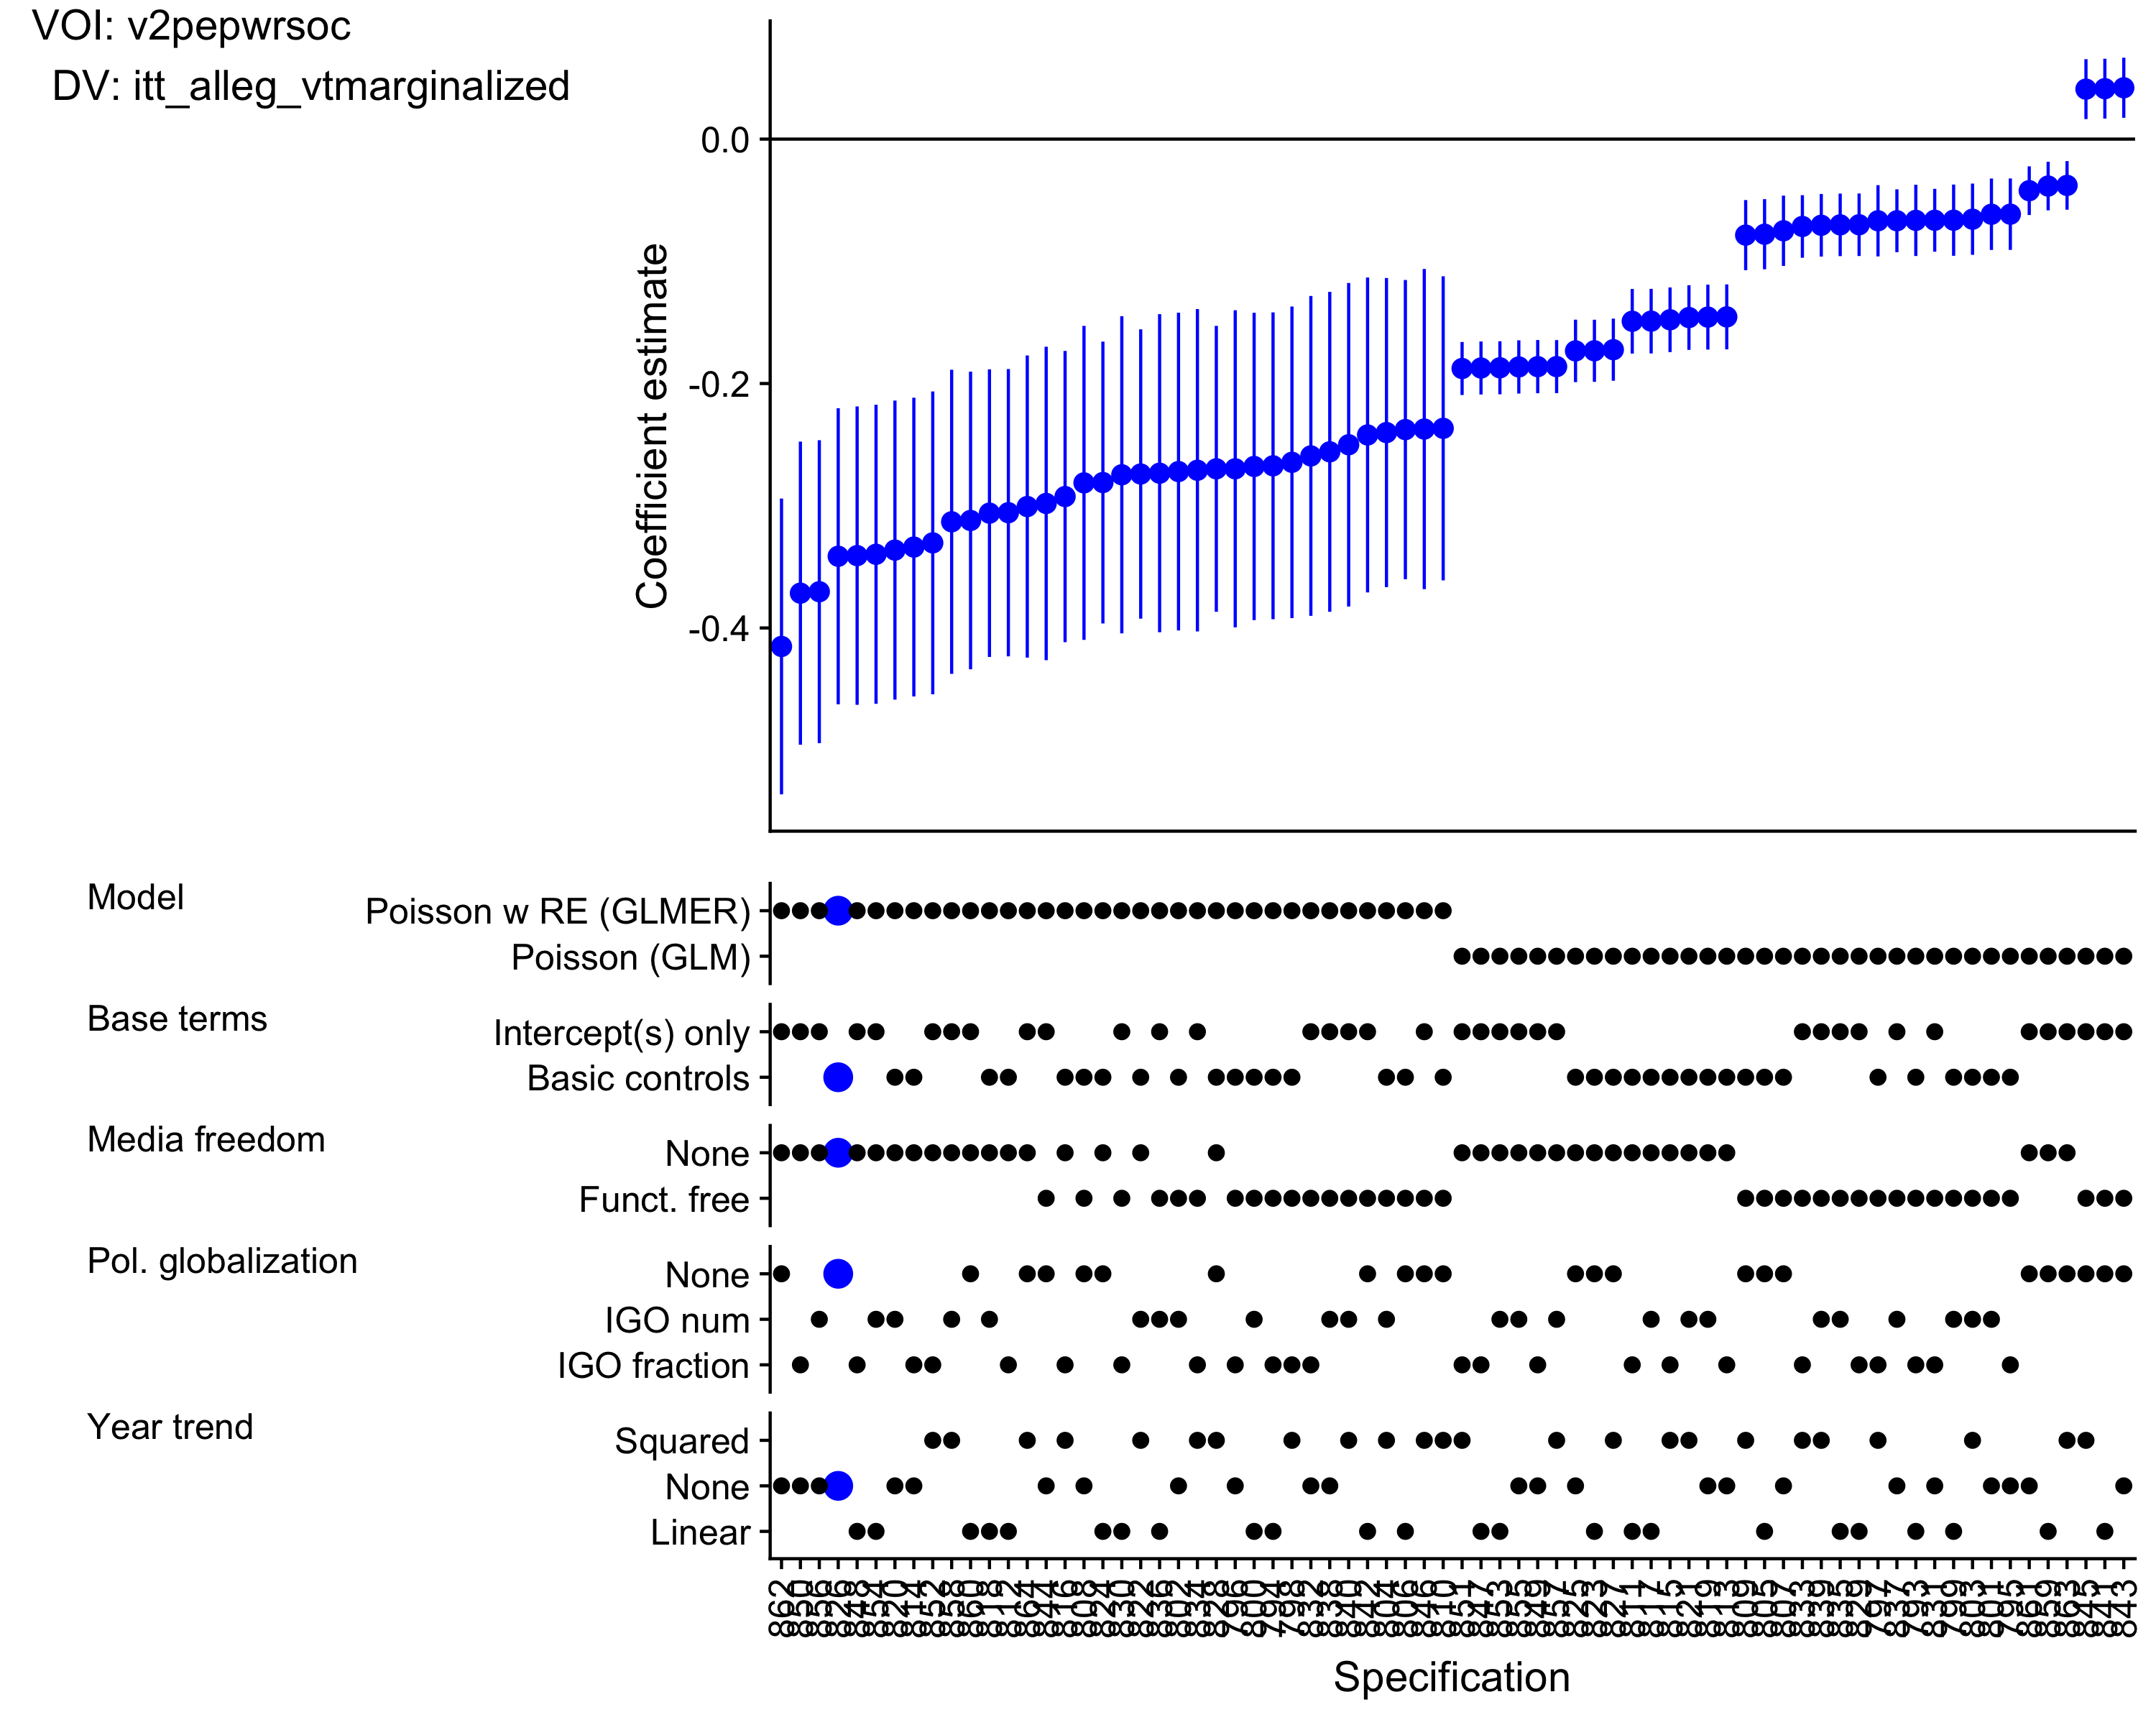
\includegraphics[height=4in]{../output/figures-robustness/specplot-v2pepwrsoc-itt_alleg_vtmarginalized.png}

\hypertarget{voi-v2x_jucon}{%
\subsection{VOI: v2x\_jucon}\label{voi-v2x_jucon}}

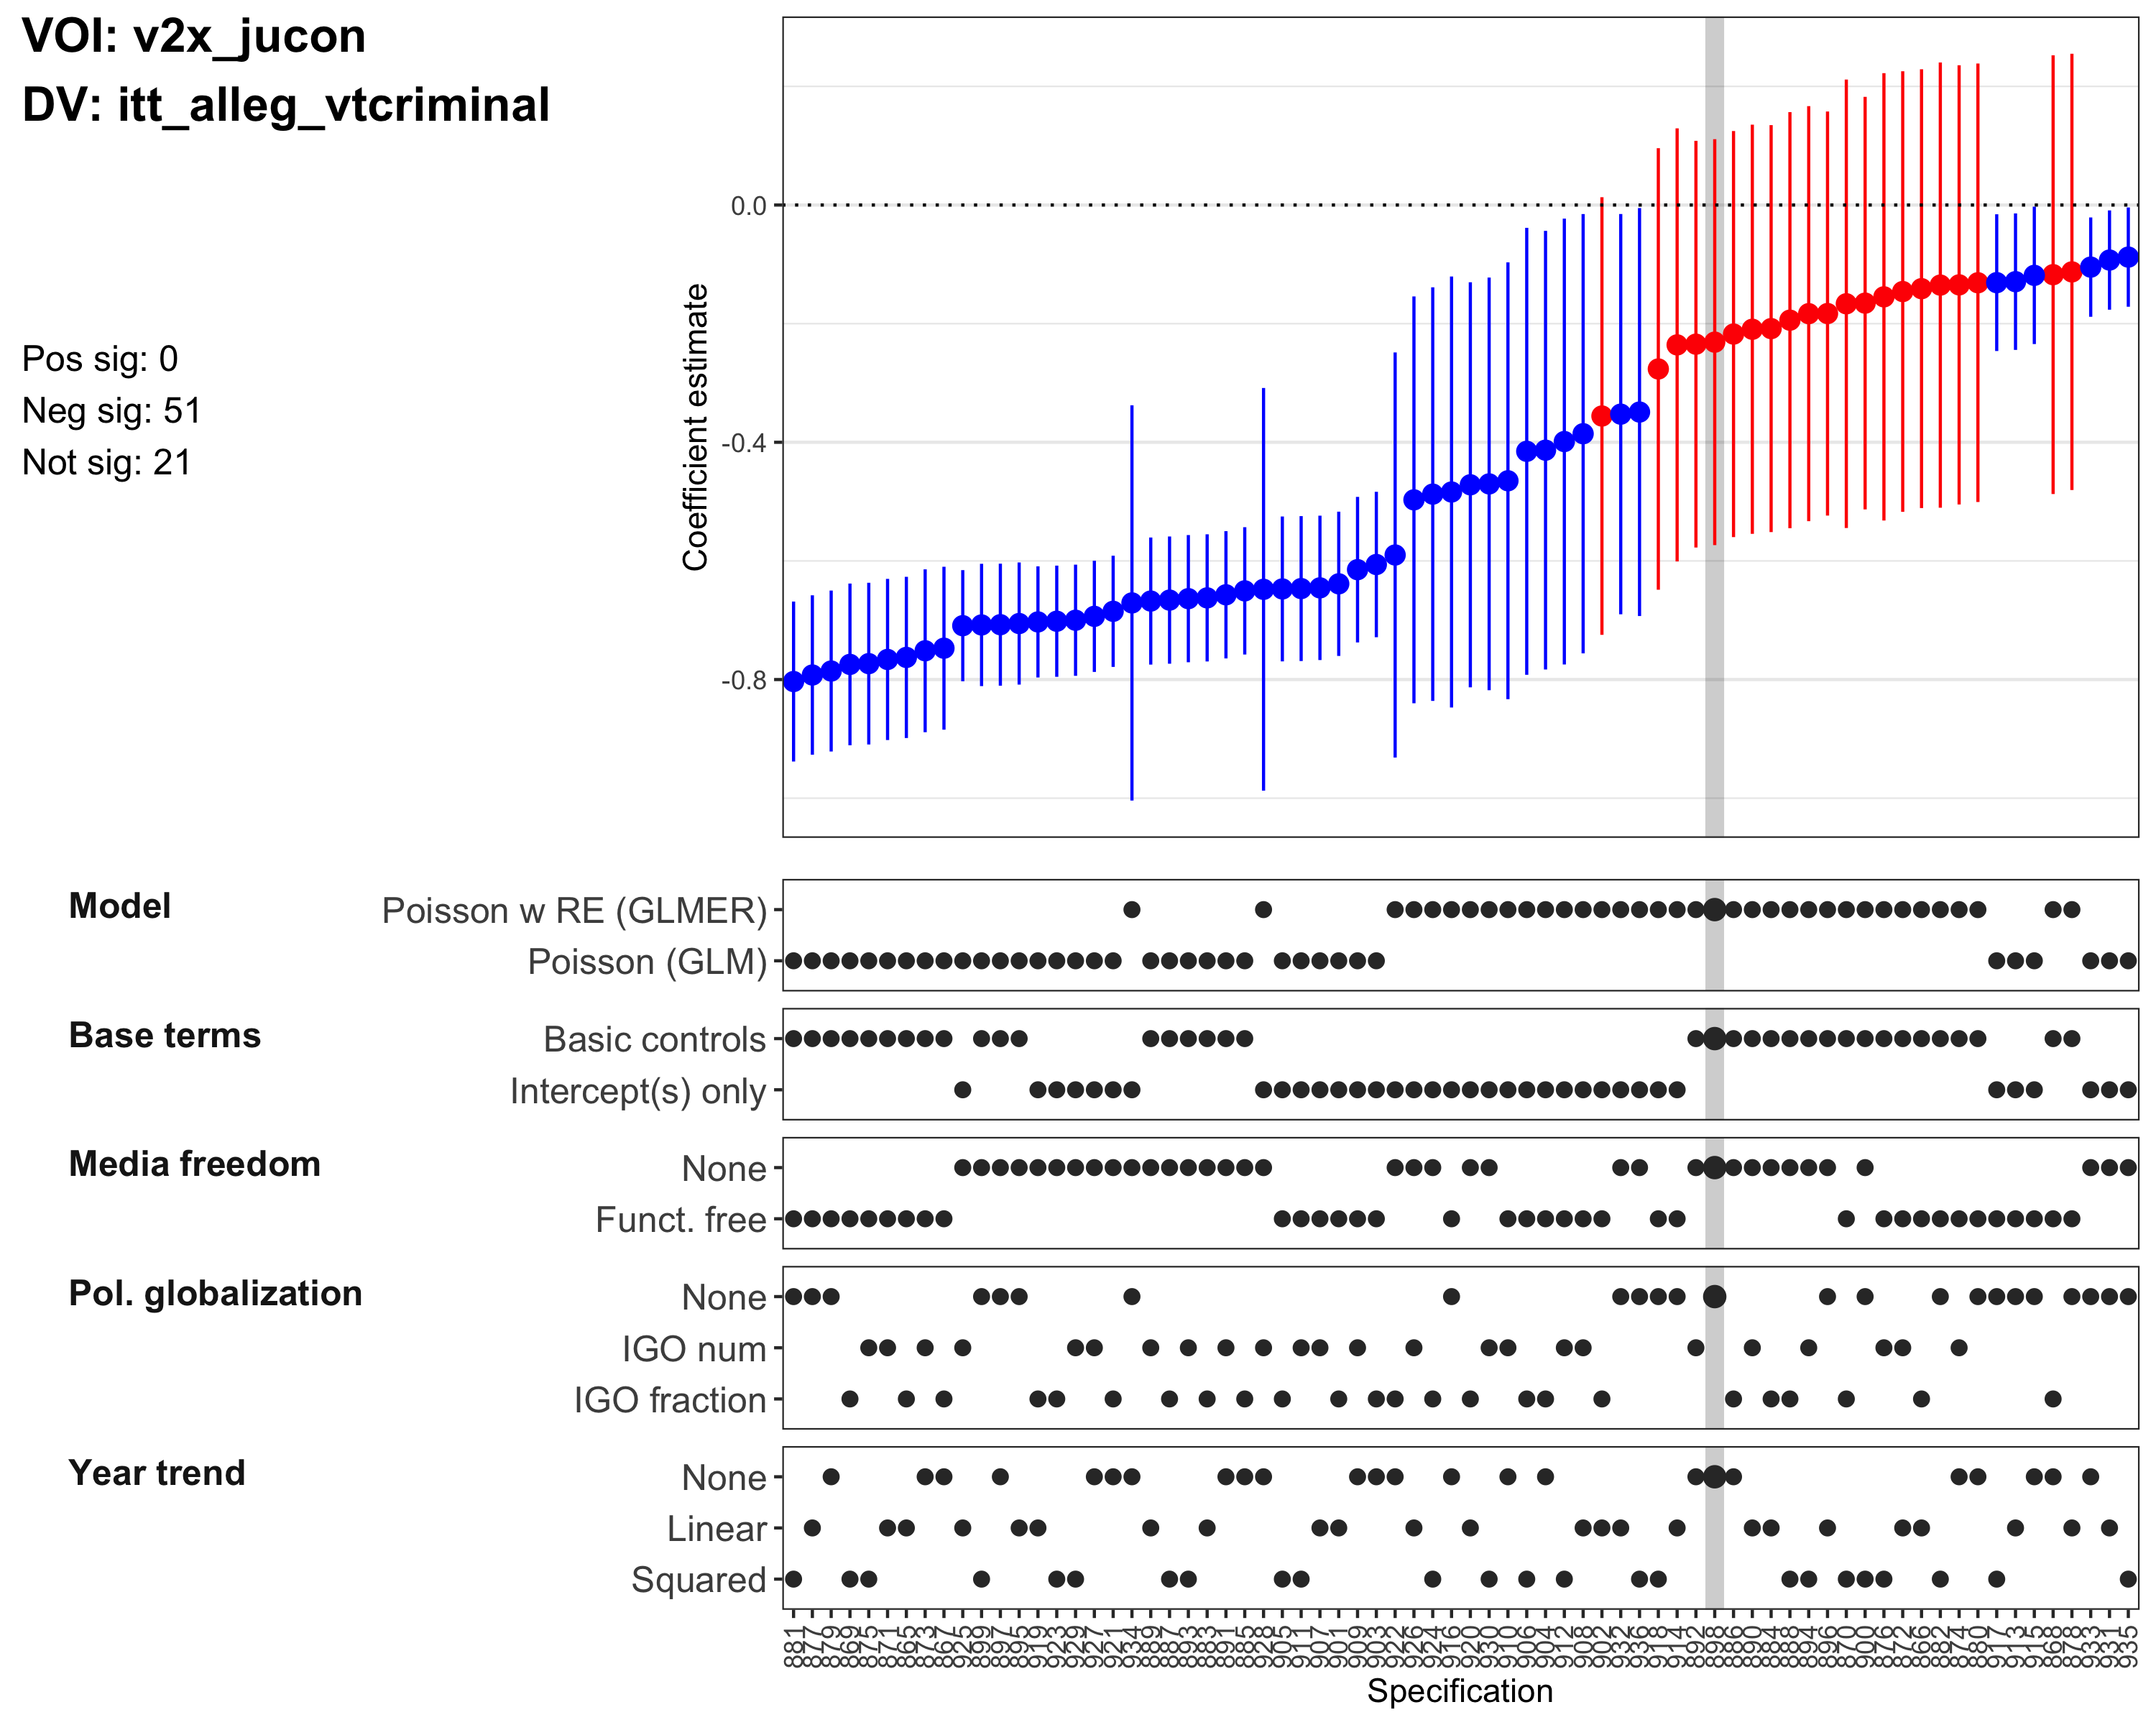
\includegraphics[height=4in]{../output/figures-robustness/specplot-v2x_jucon-itt_alleg_vtcriminal.png}

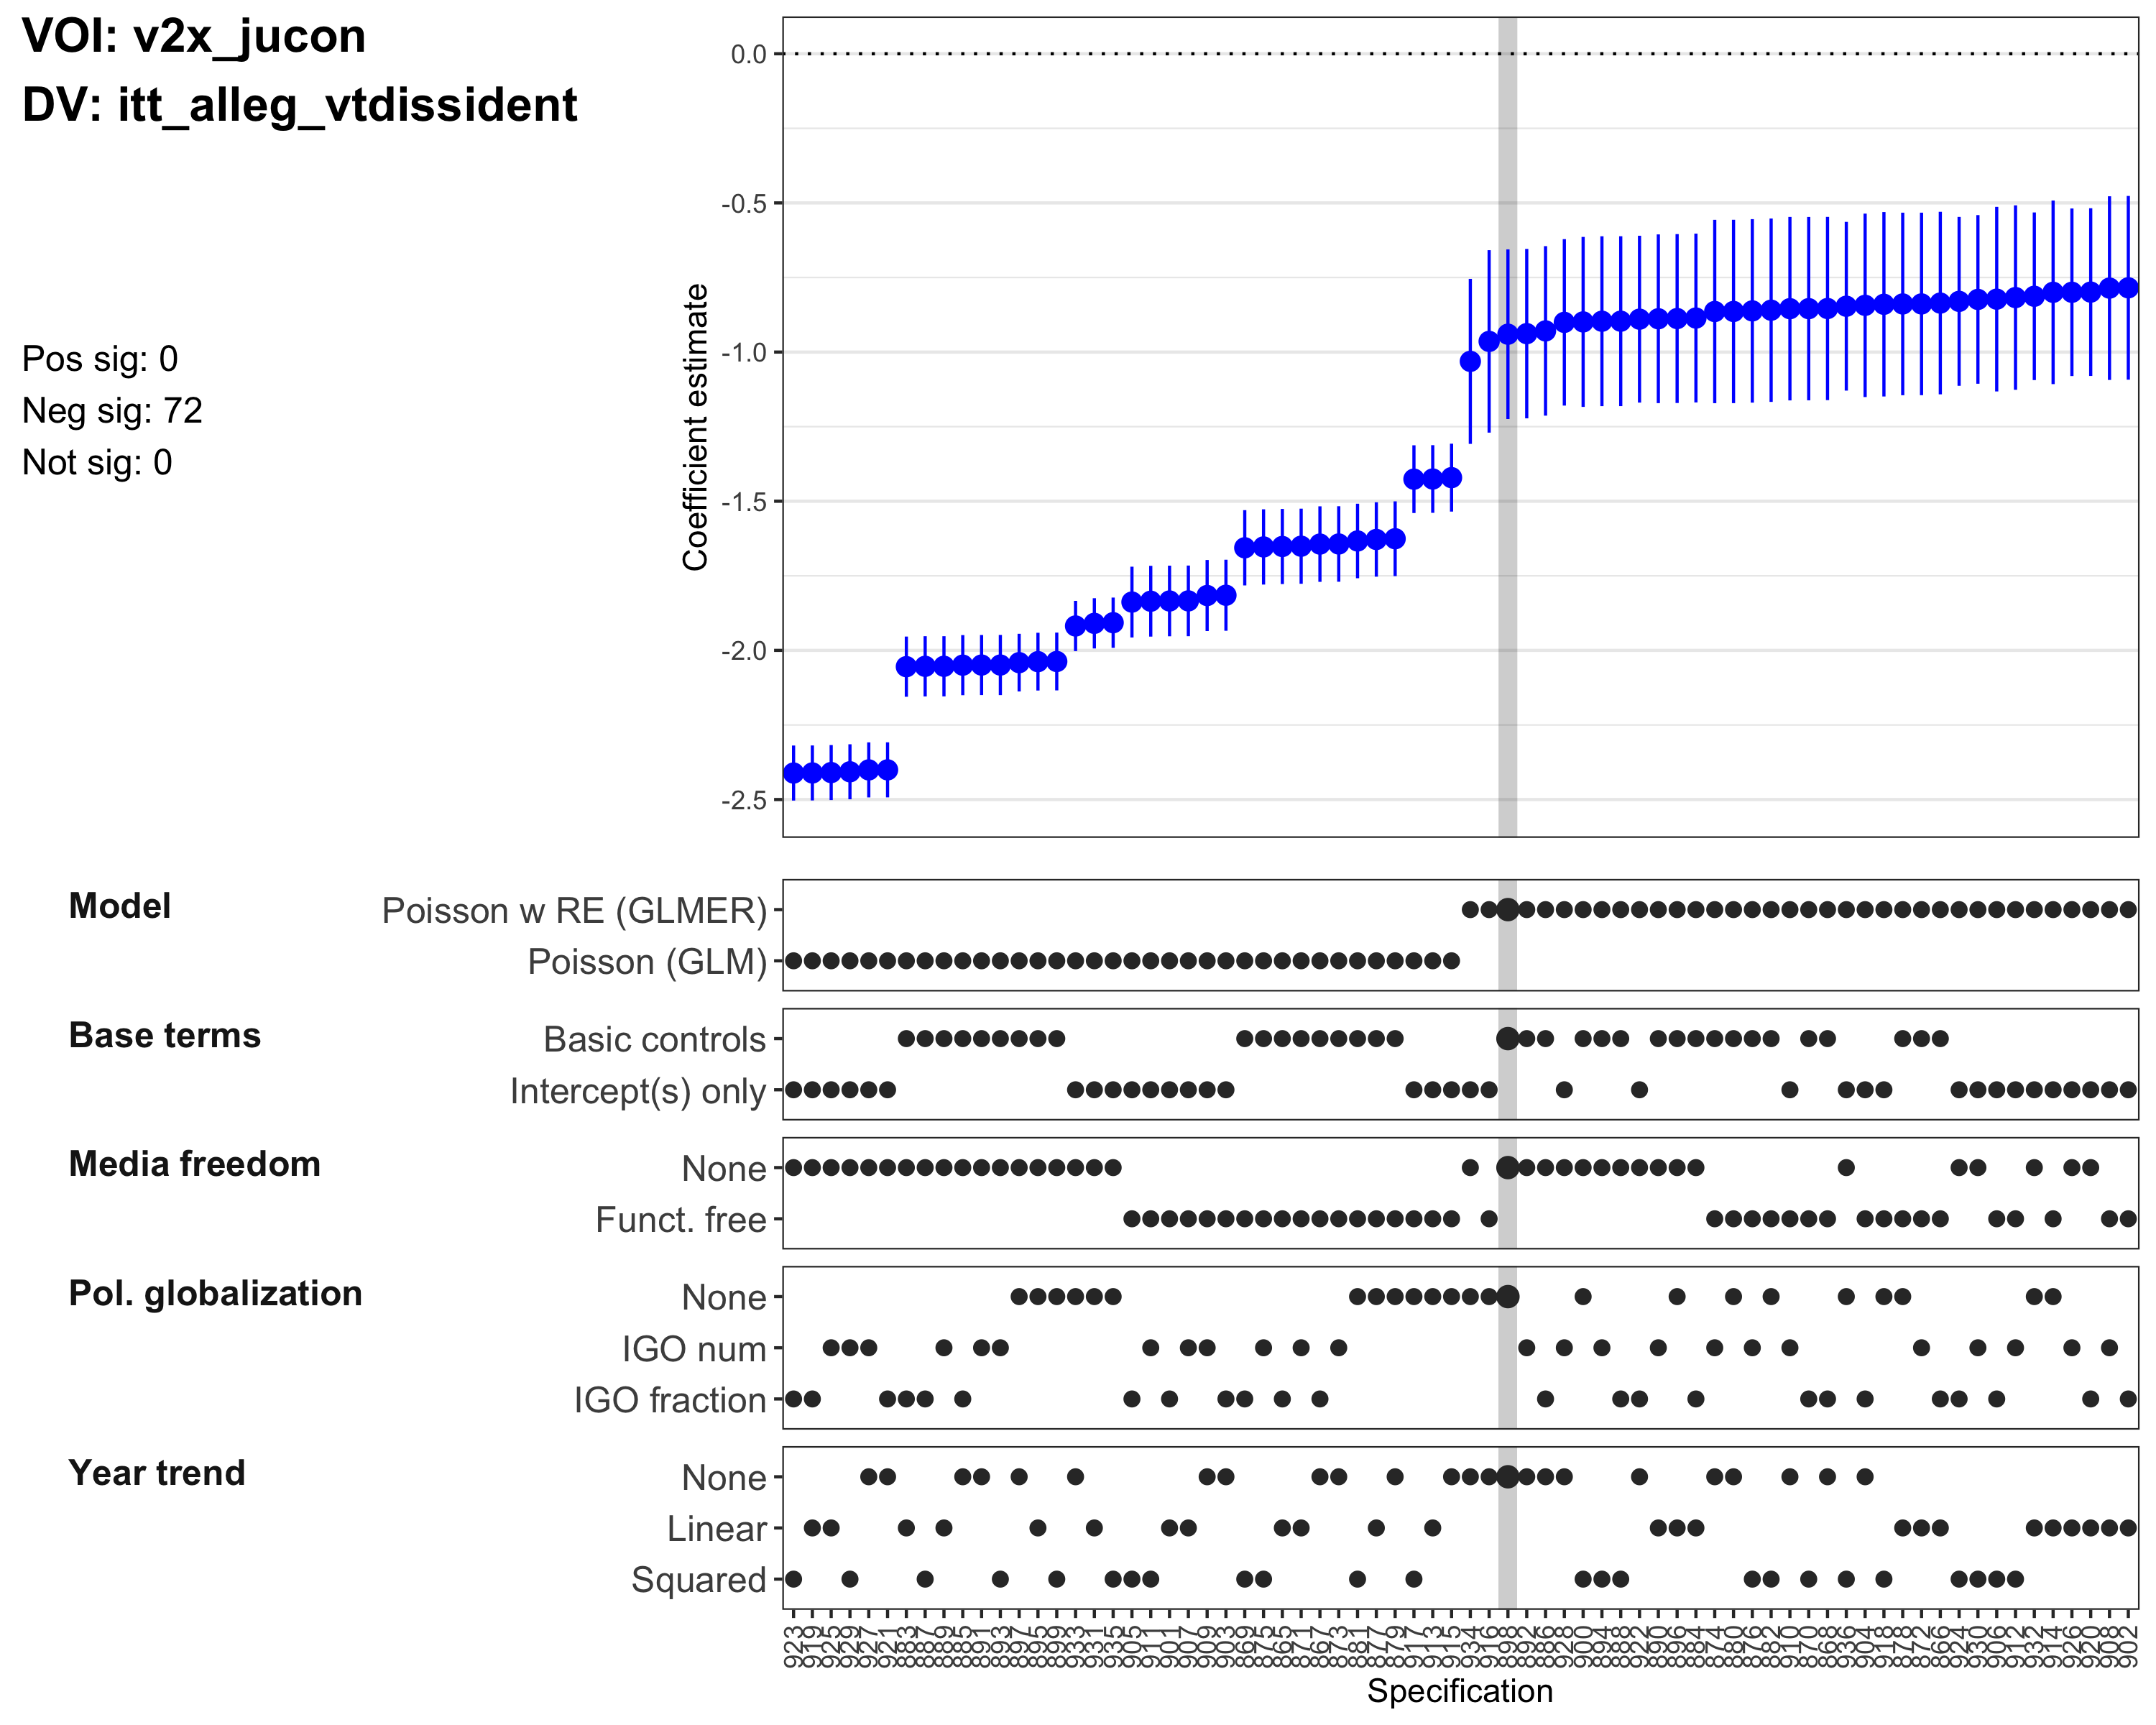
\includegraphics[height=4in]{../output/figures-robustness/specplot-v2x_jucon-itt_alleg_vtdissident.png}

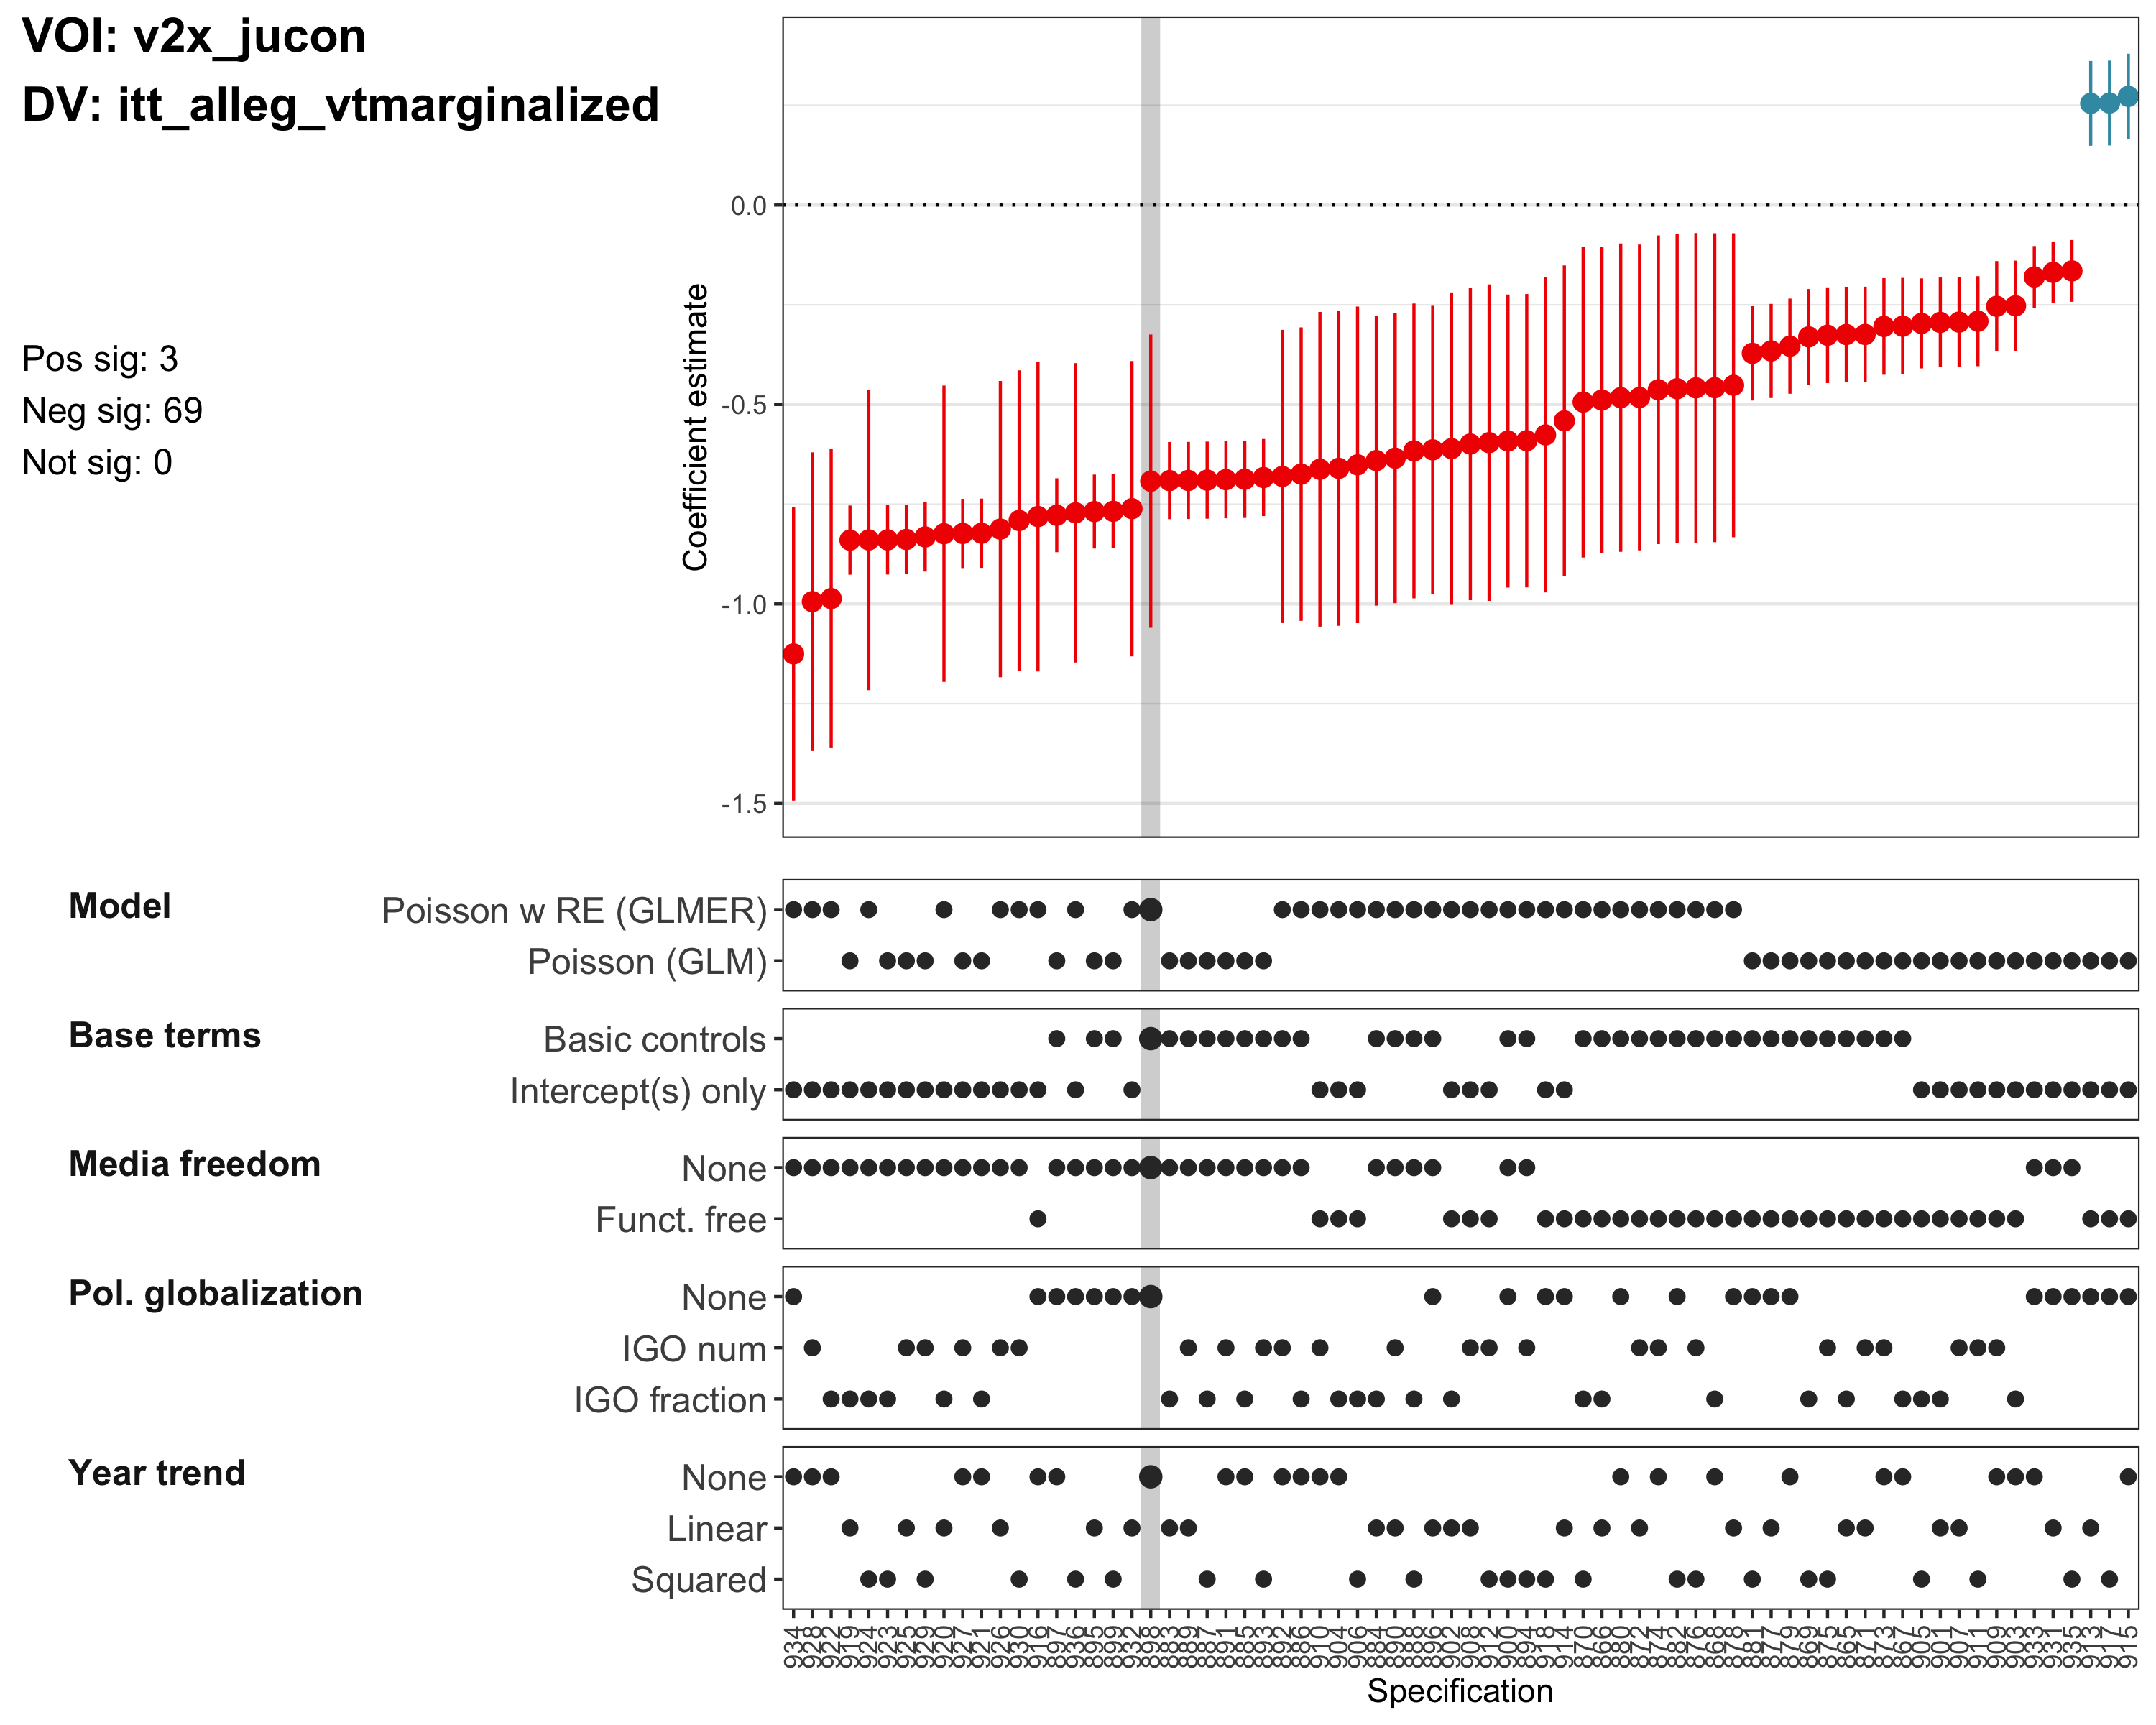
\includegraphics[height=4in]{../output/figures-robustness/specplot-v2x_jucon-itt_alleg_vtmarginalized.png}

\hypertarget{voi-v2xlg_legcon}{%
\subsection{VOI: v2xlg\_legcon}\label{voi-v2xlg_legcon}}

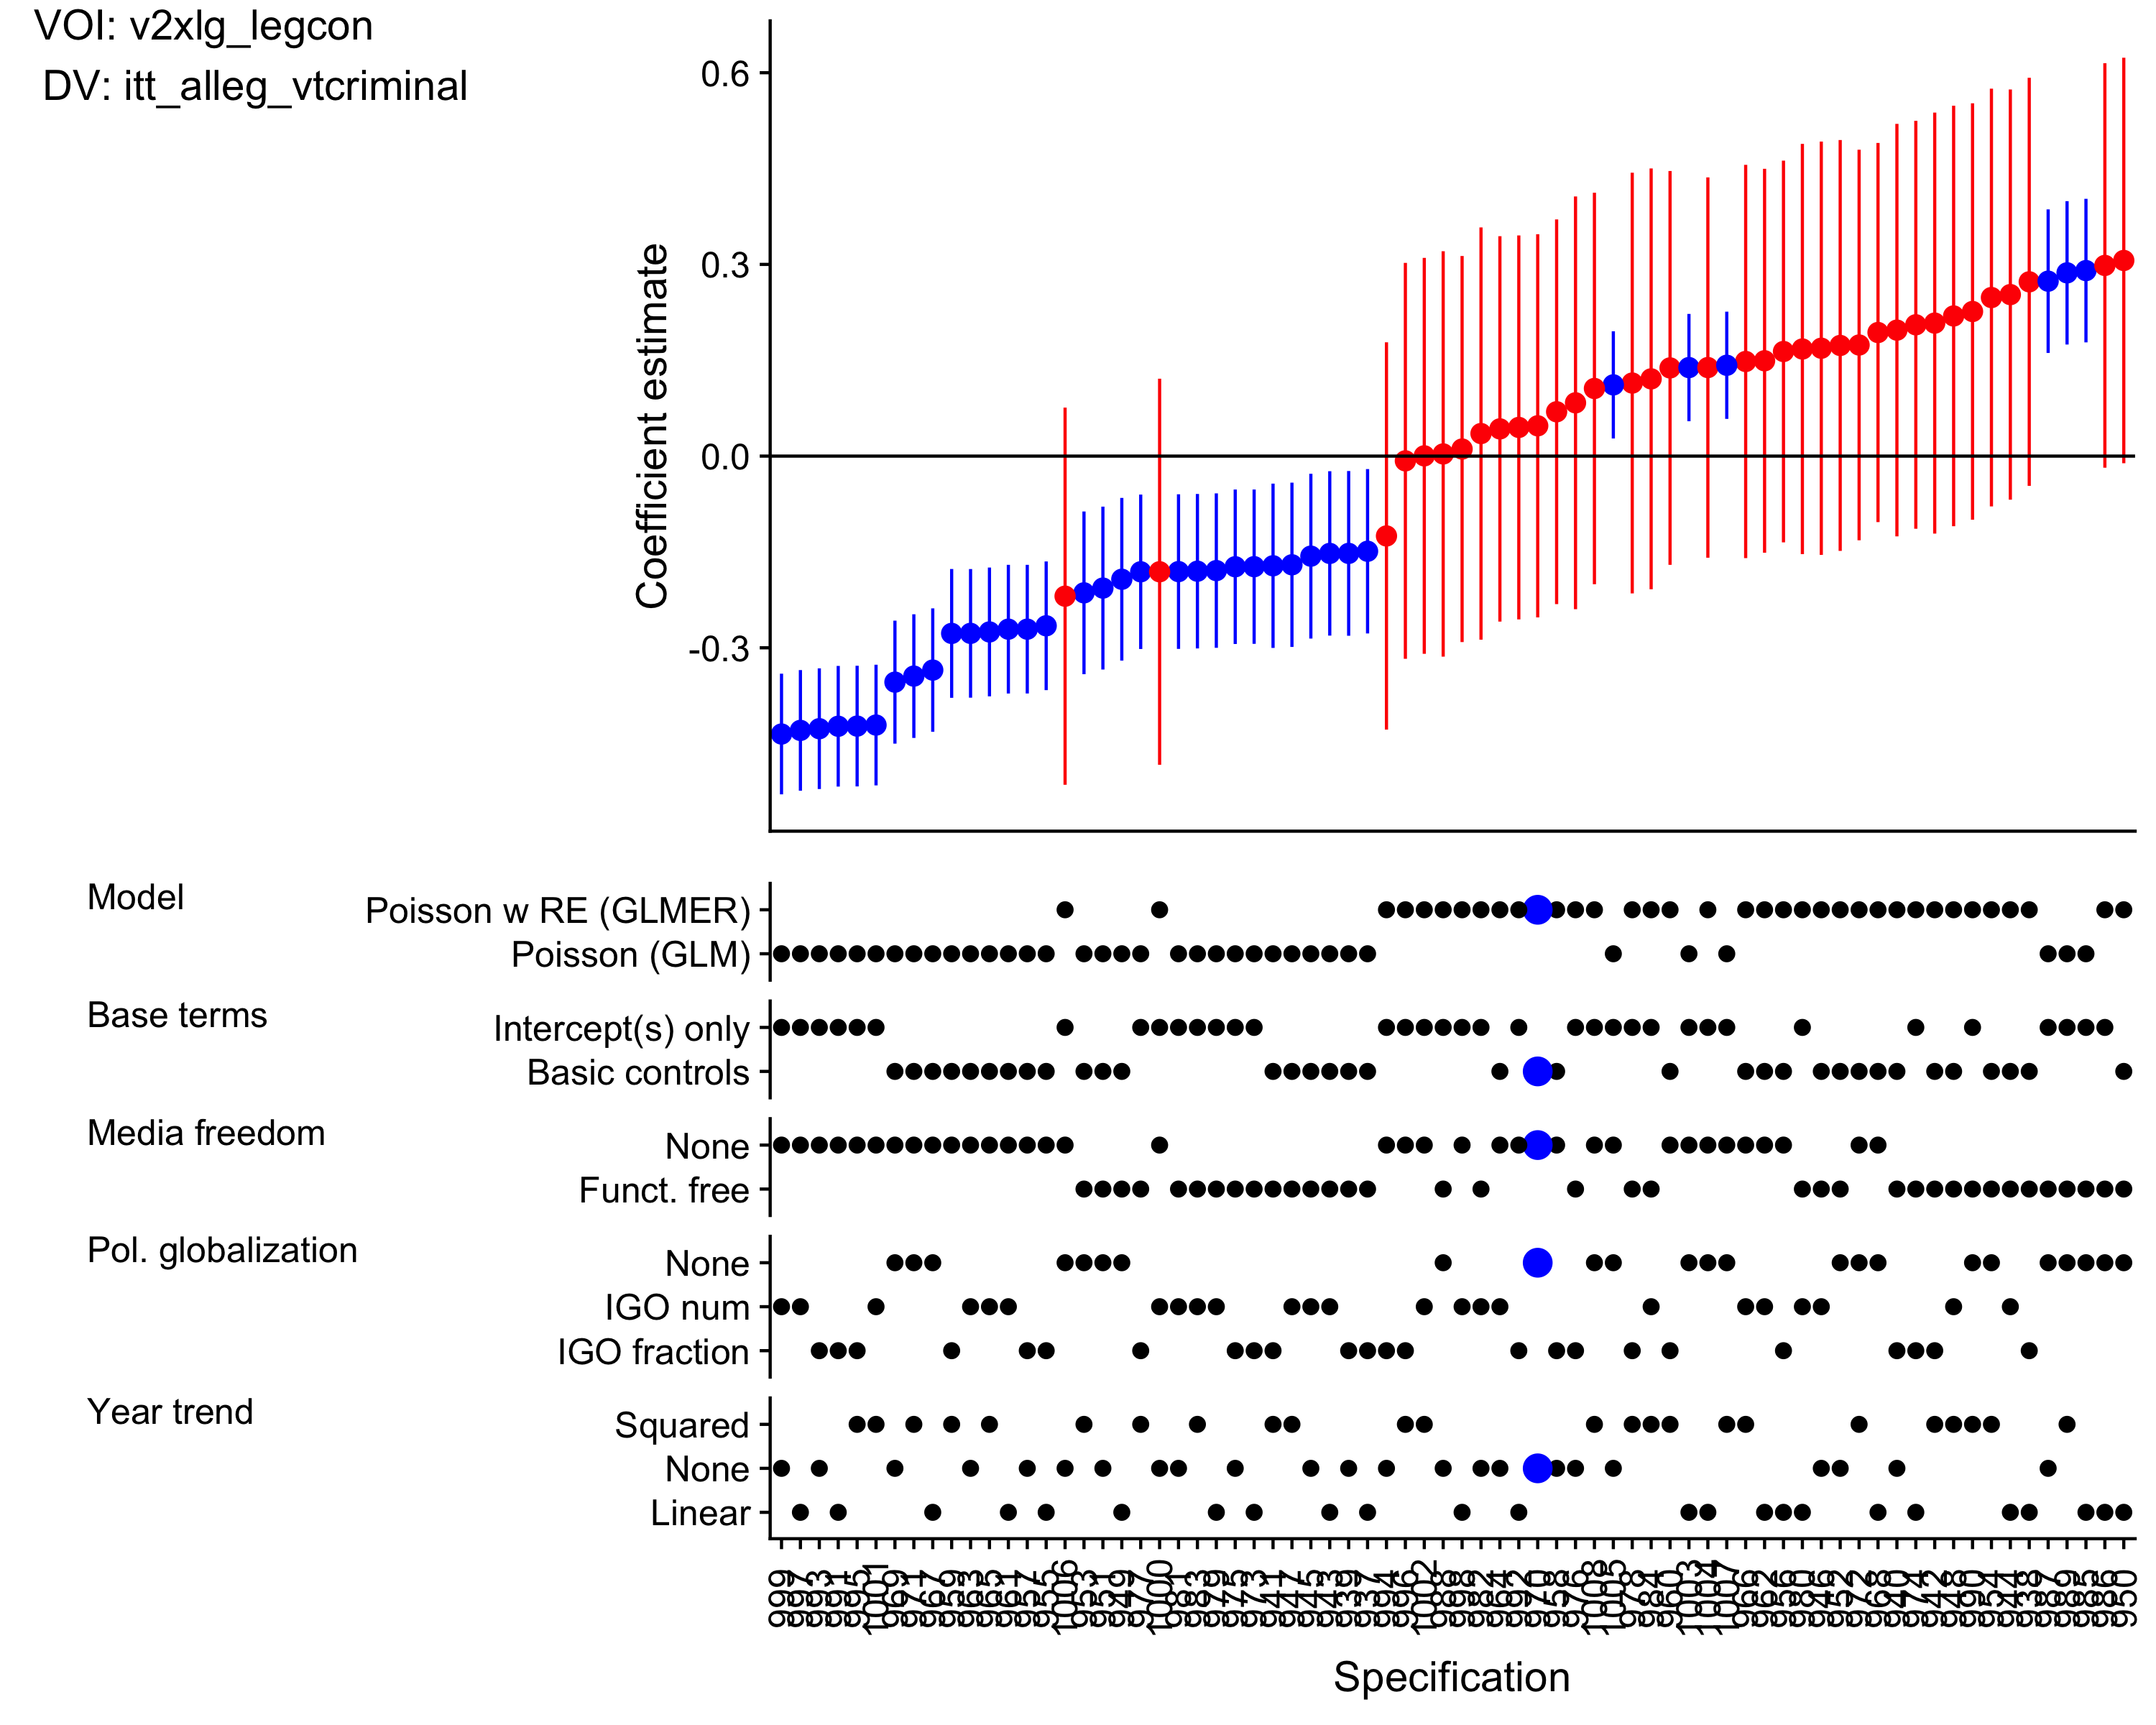
\includegraphics[height=4in]{../output/figures-robustness/specplot-v2xlg_legcon-itt_alleg_vtcriminal.png}

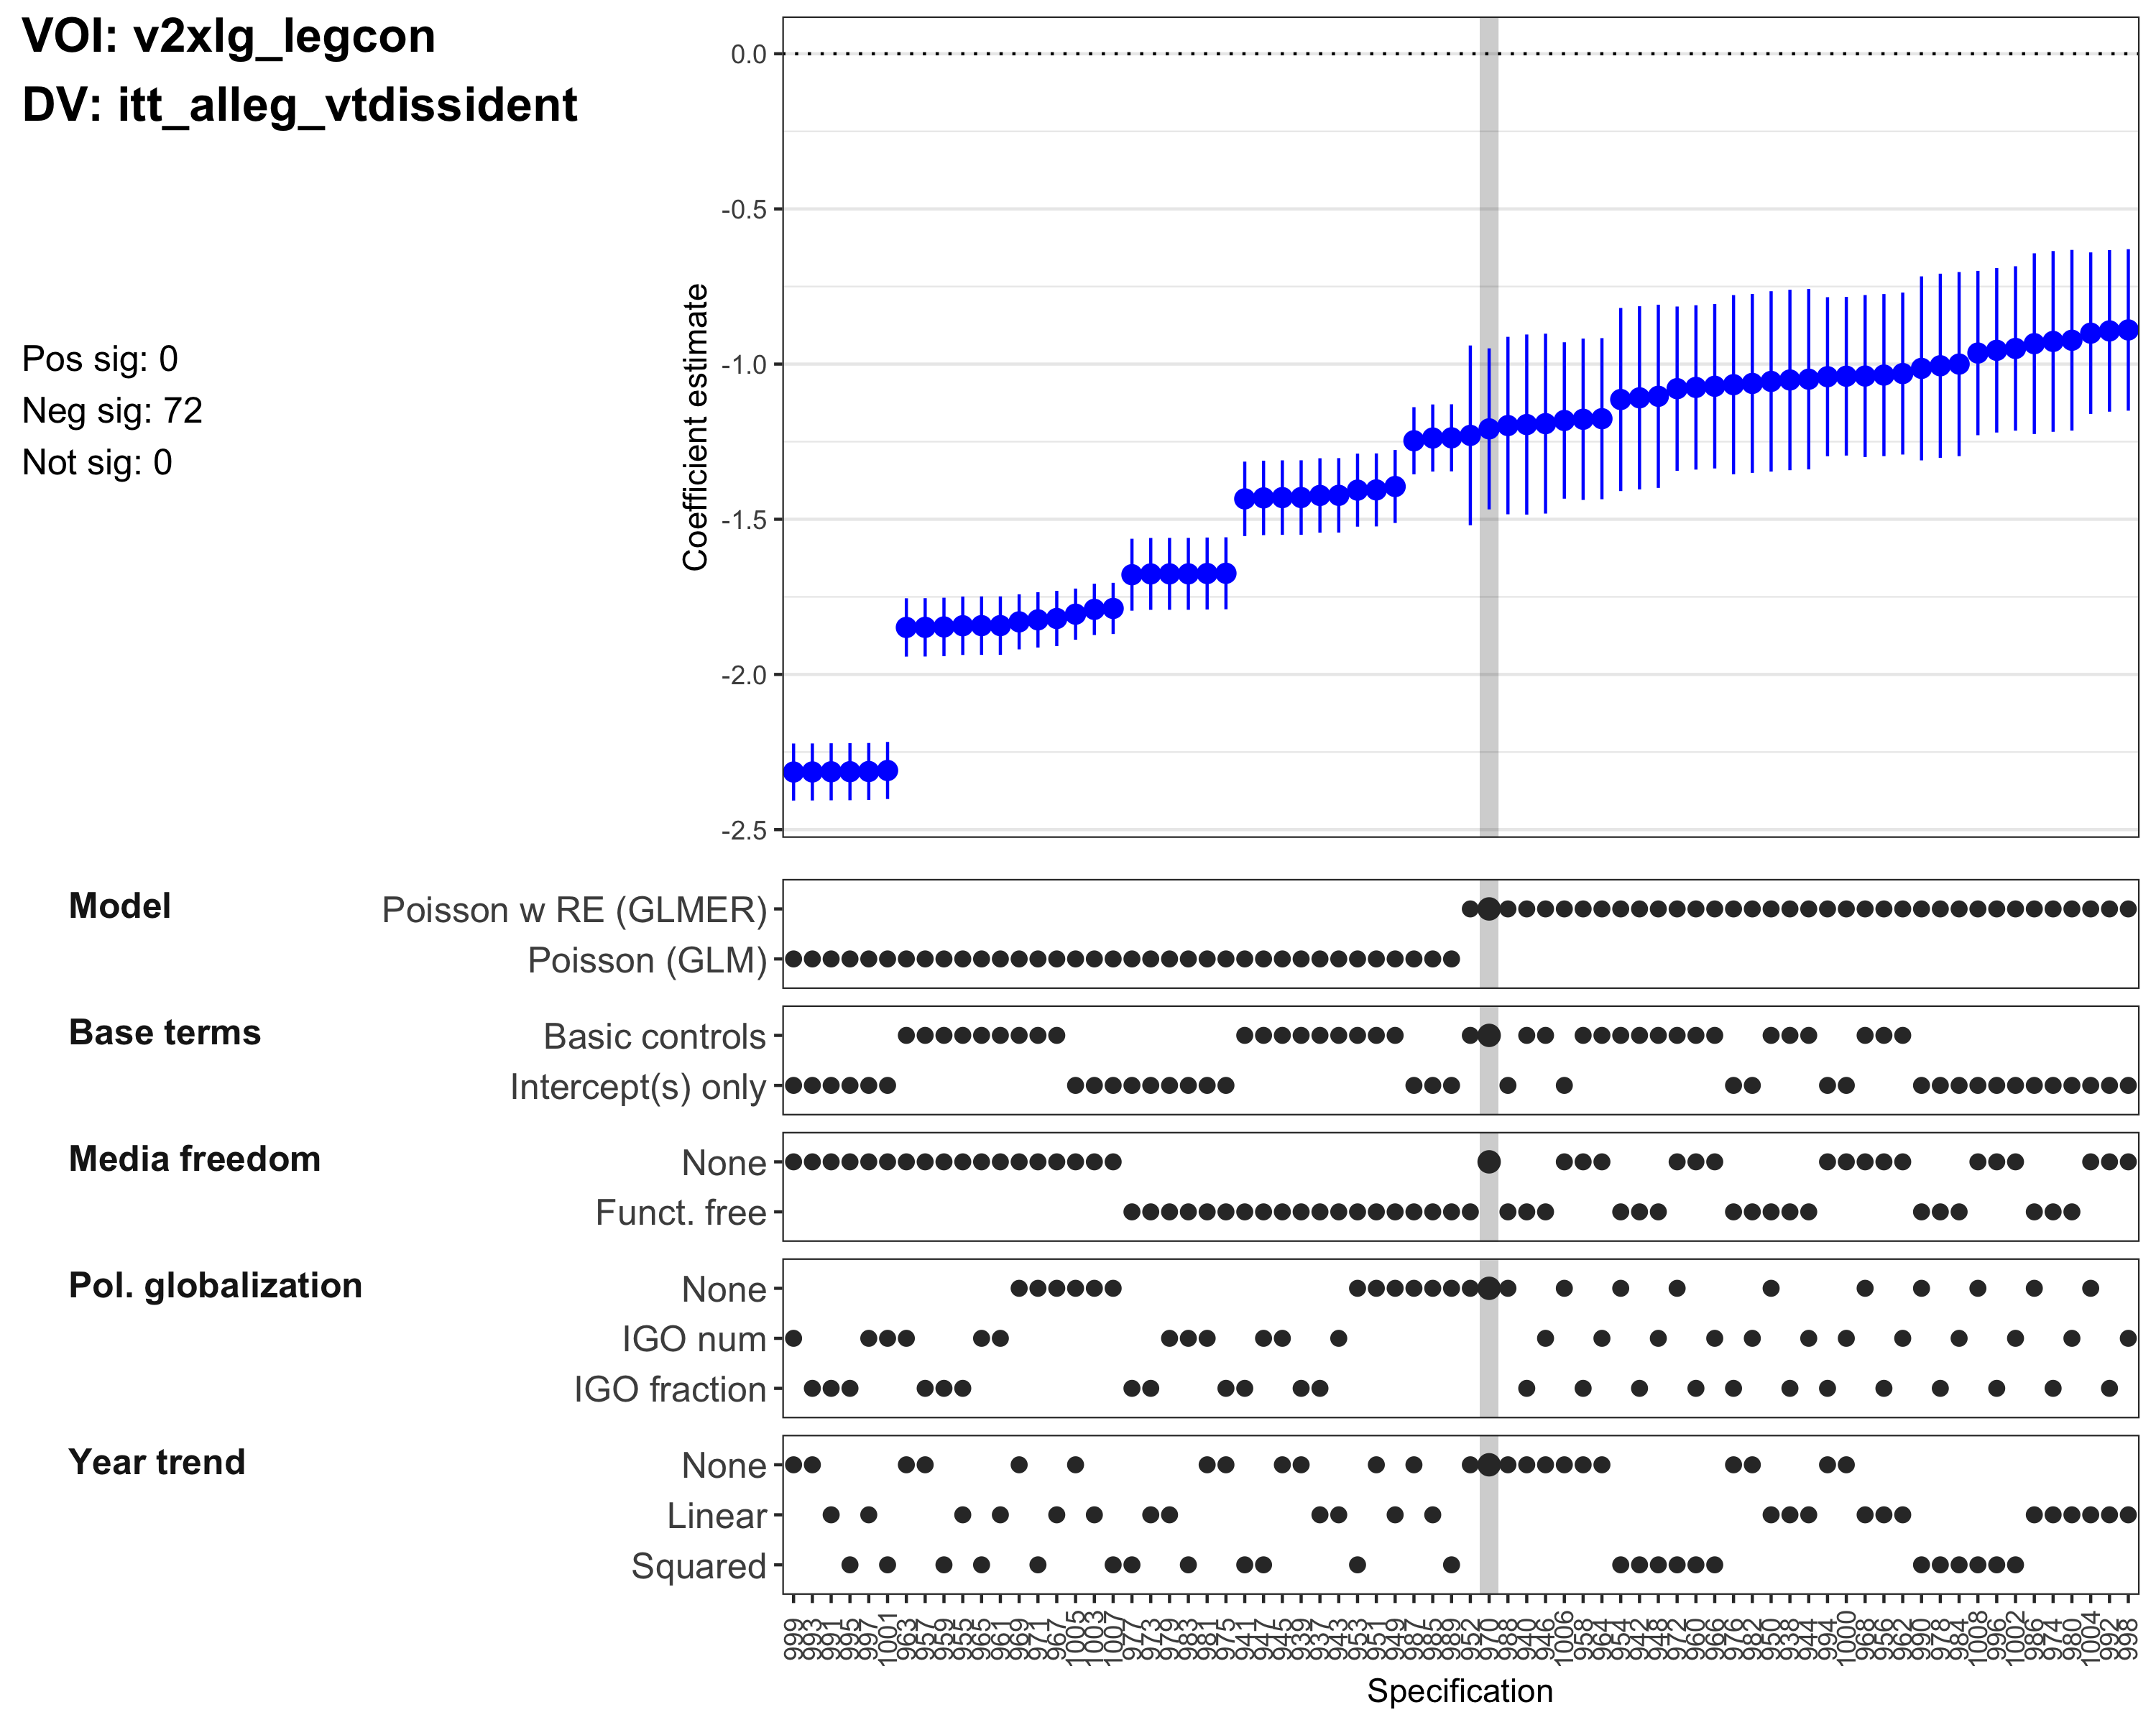
\includegraphics[height=4in]{../output/figures-robustness/specplot-v2xlg_legcon-itt_alleg_vtdissident.png}

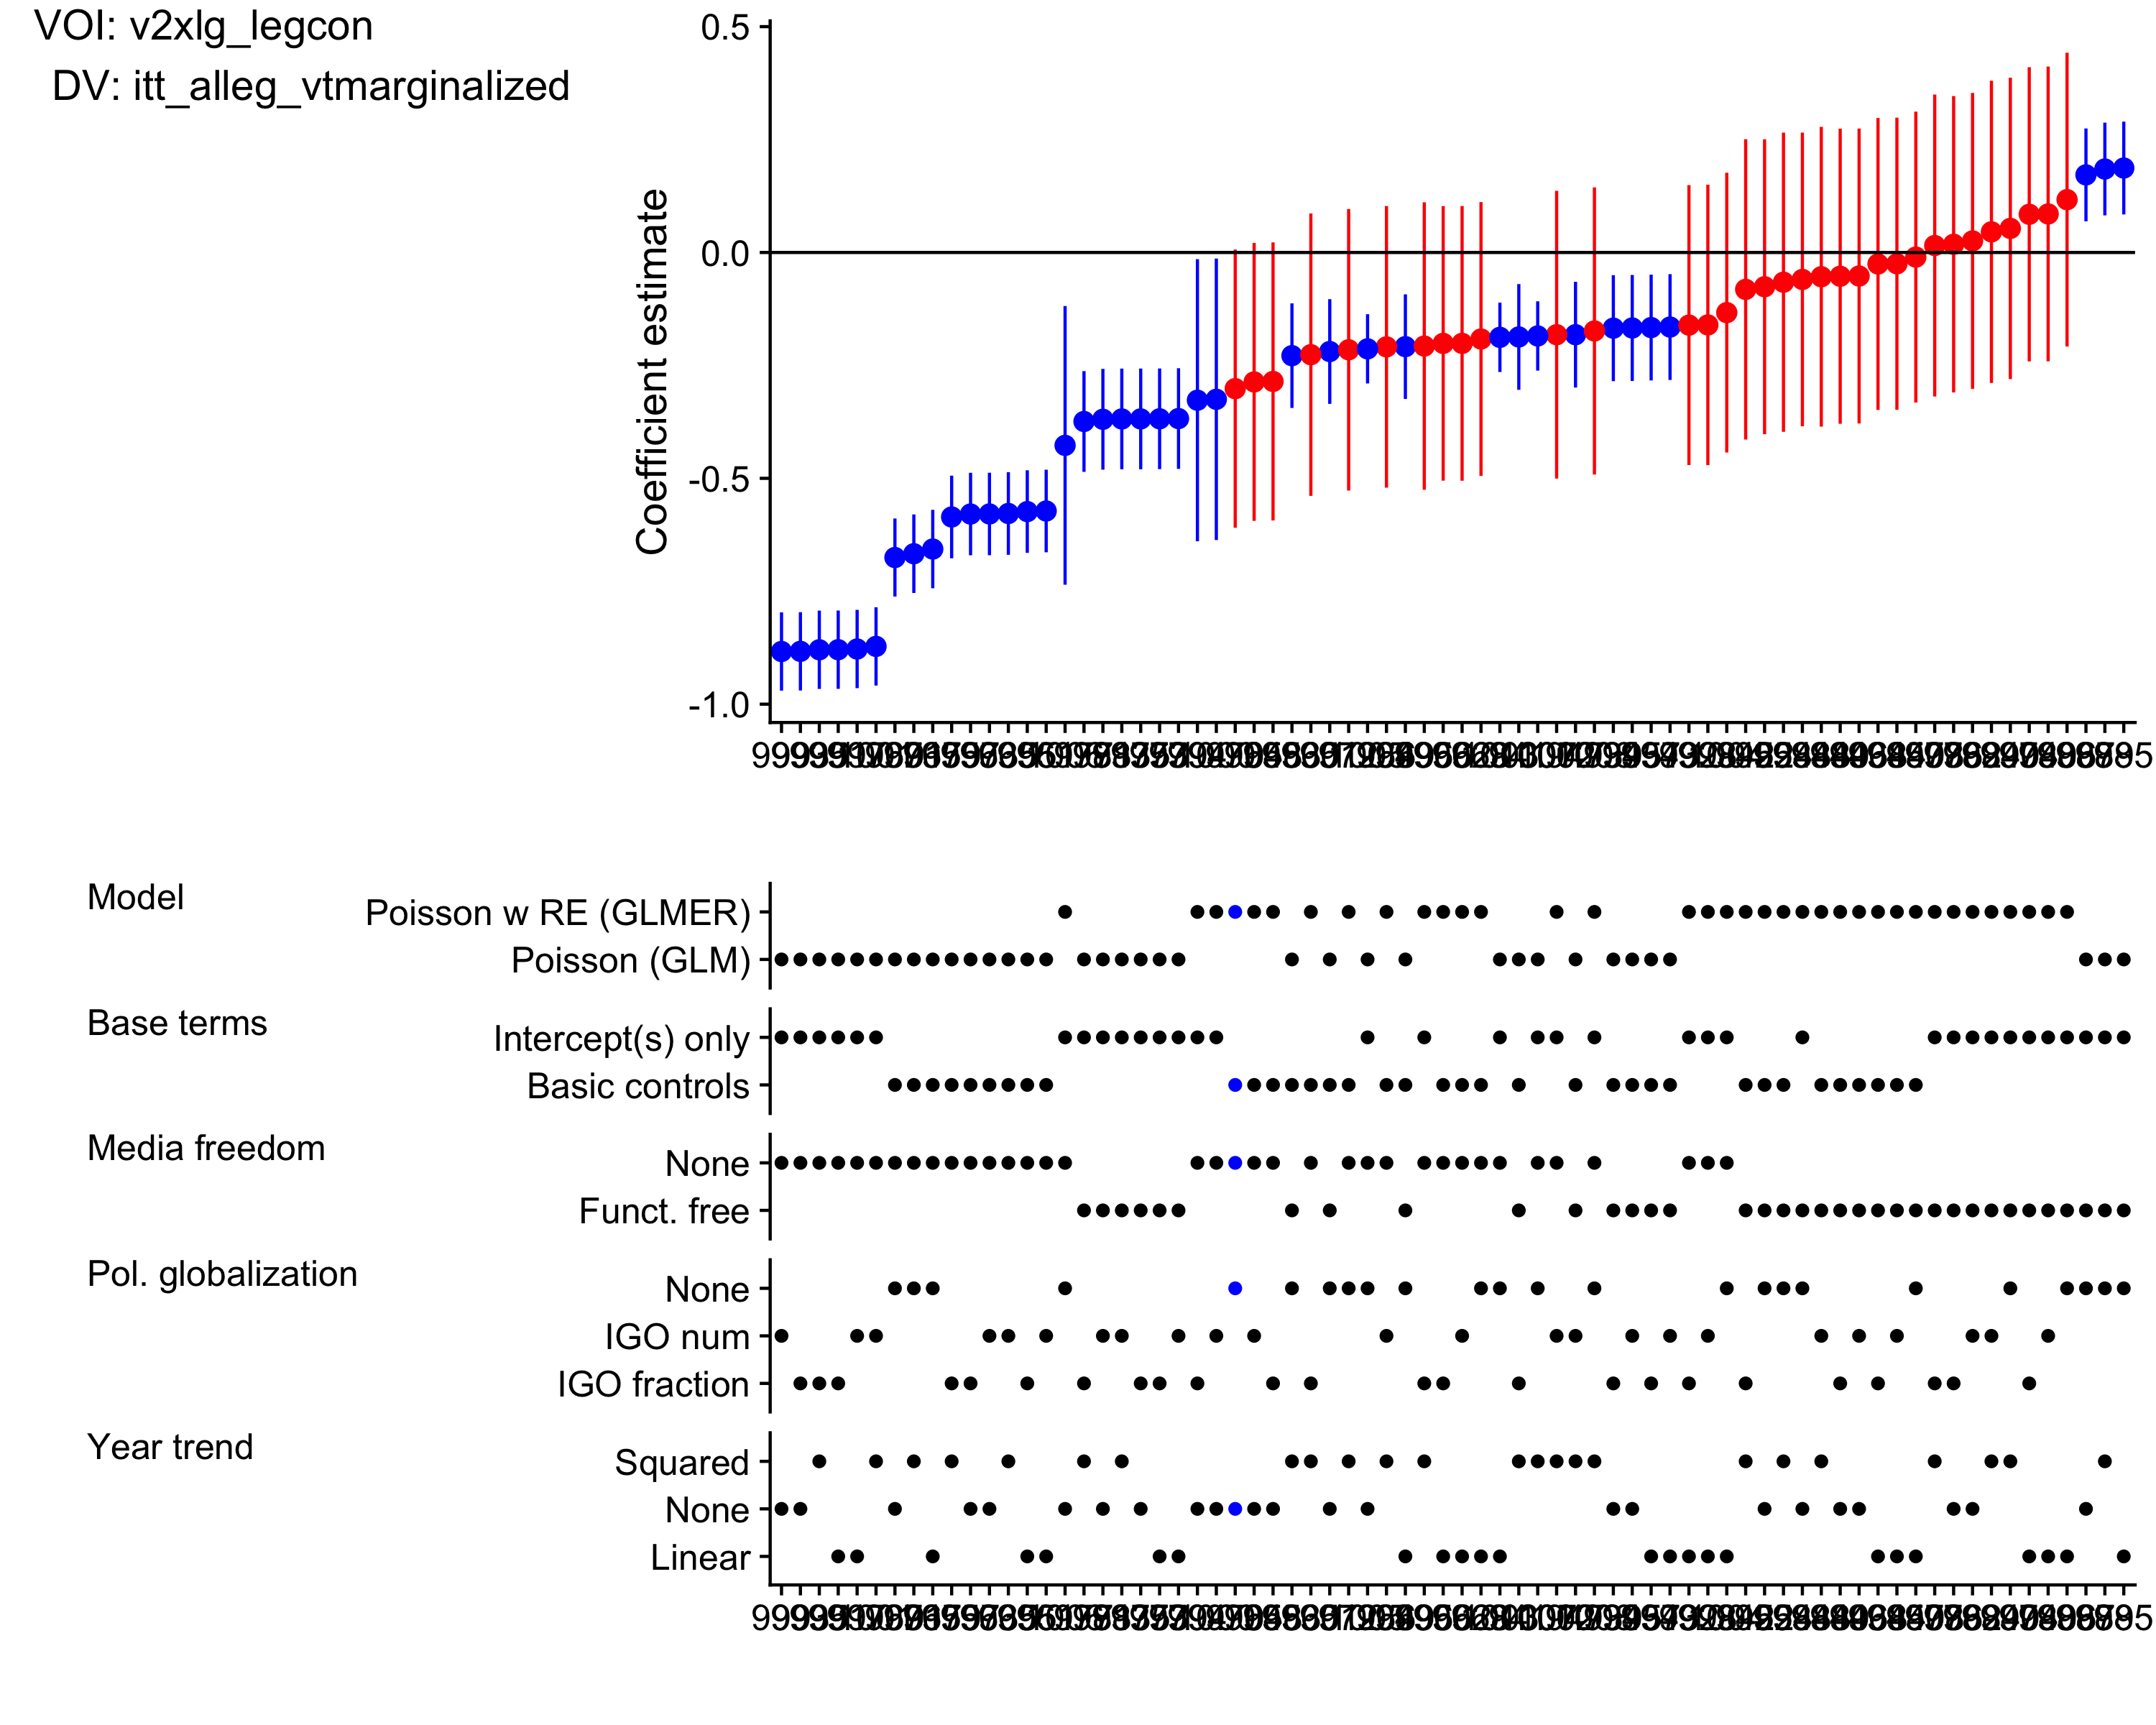
\includegraphics[height=4in]{../output/figures-robustness/specplot-v2xlg_legcon-itt_alleg_vtmarginalized.png}

\hypertarget{references}{%
\section*{References}\label{references}}
\addcontentsline{toc}{section}{References}

\hypertarget{refs}{}
\leavevmode\hypertarget{ref-gelman2013garden}{}%
Gelman, Andrew, and Eric Loken. 2013. ``The garden of forking paths.''
\url{http://www.stat.columbia.edu/~gelman/research/unpublished/p_hacking.pdf}.

\leavevmode\hypertarget{ref-murdie2012shaming}{}%
Murdie, Amanda M, and David R Davis. 2012. ``Shaming and Blaming: Using
Events Data to Assess the Impact of Human Rights Ingos.''
\emph{International Studies Quarterly} 56 (1). Blackwell Publishing Ltd
Oxford, UK: 1--16.

\leavevmode\hypertarget{ref-pevehouse2004correlates}{}%
Pevehouse, Jon, Timothy Nordstrom, and Kevin Warnke. 2004. ``The
Correlates of War 2 International Governmental Organizations Data
Version 2.0.'' \emph{Conflict Management and Peace Science} 21 (2). SAGE
Publications Sage UK: London, England: 101--19.

\leavevmode\hypertarget{ref-simonsohn2015specification}{}%
Simonsohn, Uri, Joseph P Simmons, and Leif D Nelson. 2015.
``Specification Curve: Descriptive and Inferential Statistics on All
Reasonable Specifications.'' \emph{SSRN Electronic Journal}.
\url{https://doi.org/10.2139/ssrn.2694998}.

\leavevmode\hypertarget{ref-whitten2017correlates}{}%
Whitten-Woodring, Jenifer, and Douglas A Van Belle. 2017. ``The
Correlates of Media Freedom: An Introduction of the Global Media Freedom
Dataset.'' \emph{Political Science Research and Methods} 5 (1).
Cambridge University Press: 179--88.


\end{document}
